\documentclass{dfki}
\usepackage[backend=biber]{biblatex}
\usepackage{tikz}
\usepackage{lmodern}
\addbibresource{bibliography.bib}
\title{On the effect of \newline realistic noise models on performance \newline predictions of quantum computers}
\subtitle{Spring Retreat Talk}
\author{Leon Wichette}
\date{\today}

\begin{document}
\selectfont

\setbeamertemplate{background}{
\includegraphics[width=\paperwidth]{fig/bg.pdf}}%
\begin{frame}[plain]
\titlepage\end{frame}

\setbeamertemplate{background}{}

\begin{frame}{Towards large scale QC}
	\begin{minipage}[t]{0.59\textwidth}
		\vspace{0.05cm}
		\centering
		Expected error rates on QC by advancements in optimal control $\sim 10^{-4}$ \citeauthoryear{RiverLaneRep2024}\\ %https://www.thp.uni-koeln.de/kastoryano/ExSheets/Notes_v5.pdf
		\vspace{0.3cm}
		{\textbf{vs.}} \\
		\vspace{0.3cm}
		Desirable error rates for large scale applications $\sim 10^{-14}-10^{-15}$ \citeauthoryear{fowler_surface_2012}\\
	\end{minipage}
	\hfil
	\begin{minipage}[t]{0.4\textwidth}
		\vspace{-2.2cm}
		\hspace{1.5cm}
        
\includegraphics[width=0.6\textwidth]{fig/Noise.png}
    \end{minipage}
	\pause
	\only<2->{
		\begin{textblock*}{5.8cm}(9.8cm,4.4cm)
			\begin{tcolorbox}[colback=yellow!20, colframe=black, title=Classical computer]
				Average error rate $\sim 10^{-18}$ %https://www.thp.uni-koeln.de/kastoryano/ExSheets/Notes_v5.pdf
			\end{tcolorbox}
		\end{textblock*}
	}
	\pause
	\vspace{0.8cm}
	\begin{center}
		\begin{tcolorbox}[colback=osakared!5!white, colframe=osakared, width=13cm, arc=2mm]
			\center
			$\Rightarrow$ Error correction is necessary for large scale quantum applications
		\end{tcolorbox}
	\end{center}
\end{frame}

\begin{frame}{Classical vs. Quantum Error Correction}
	Error correction is well studied in classical setting but there exist obstacles to transfer existing methods to quantum setting:
	\begin{center}
        \begin{tabular}{p{7cm}|p{7cm}}
            \textbf{Classical Error Correction} & \textbf{Quantum Error Correction} \\
			\vspace{0.5cm}\\
            Can copy data & No-cloning theorem \\
			\vspace{0.5cm}\\
            Can measure data without disturbance & Projective measurement changes state \\
			\vspace{0.5cm}\\
            Only bit-flip errors & Bit- and phase-flip errors \\
        \end{tabular}
    \end{center}
\end{frame}

\begin{frame}{QEC general idea}
	\begin{minipage}[t]{0.65\textwidth}
		\centering
		\textbf{Error correction code:}
		\hspace{1cm}
		\raisebox{-0.3cm}{
\includegraphics[width=0.15\textwidth]{fig/single_qubit.png}}
		\hspace{1cm}
		$\hat{=}$
		\hspace{1cm}
	\end{minipage}
	\begin{minipage}[t]{0.3\textwidth}
		\vspace{-1.5cm}
        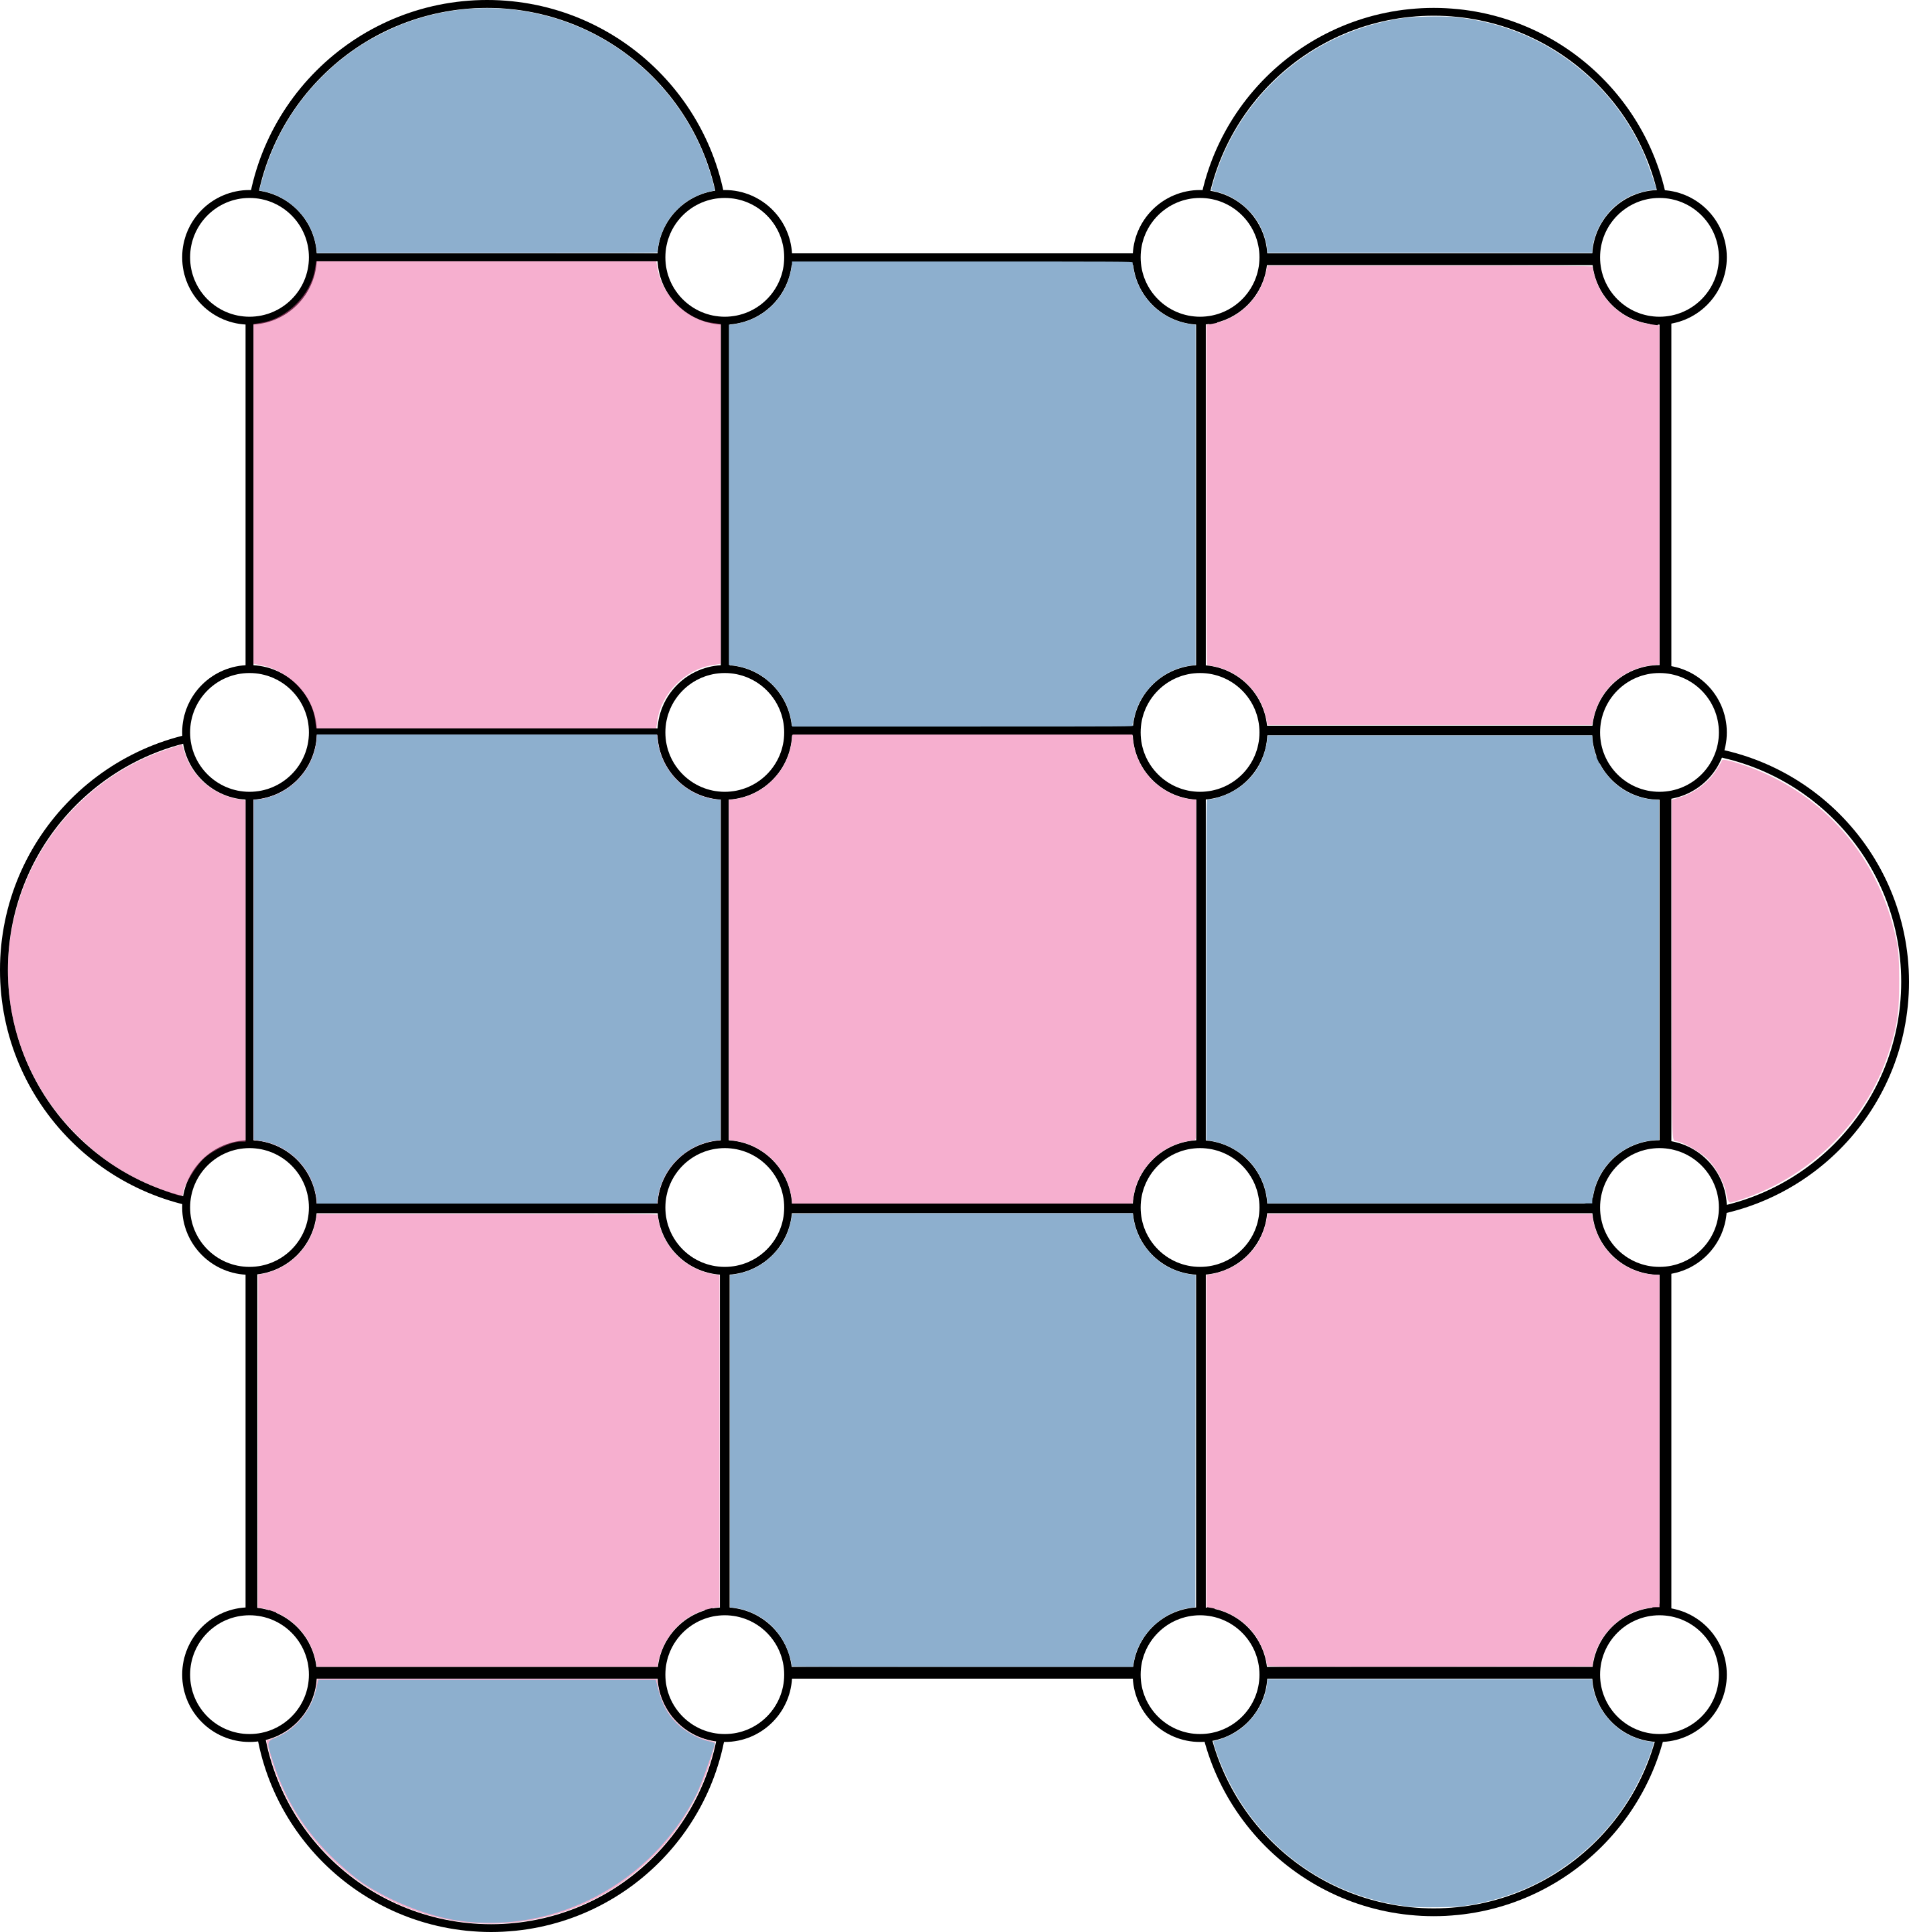
\includegraphics[width=0.6\textwidth]{fig/Rotated_surface_code_d4.png}
    \end{minipage}
	\pause
	\begin{tikzpicture}[overlay]
        \draw[-, line width=0.8mm, osakared] (-3.2, -1.2) -- (-3.2, -1.6);
        \draw[-, line width=0.8mm, osakared] (-3.17, -1.6) -- (-10.03, -1.6);
        \draw[->, line width=0.8mm, osakared] (-10, -1.6) -- (-10, -3.5);
    \end{tikzpicture}
	\begin{tikzpicture}[overlay]
        \draw[<-, line width=0.8mm, osakared] (-2.5, -1.2) -- (-2.5, -3.5);
    \end{tikzpicture}
	\par
	\vspace{1.5cm}
	\hspace{0.8cm}
	\textbf{Decoder:}
	\vspace{-1cm}
	\begin{center}
		Partial error information
		\hspace{0.5cm}
		\raisebox{-5pt}{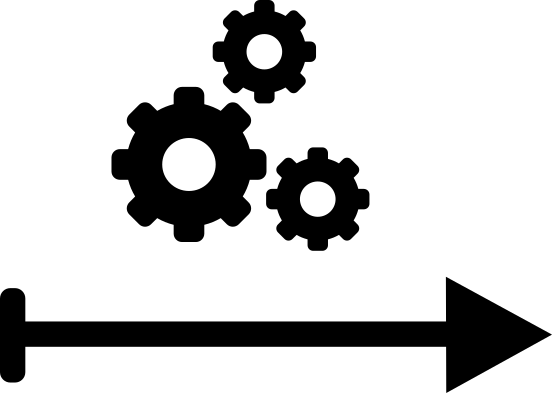
\includegraphics[width=0.2\textwidth]{fig/classical_algorithm.png}}
		\hspace{0.5cm}
		correction operation
	\end{center}
	\pause
	\only<3-3>{
		\begin{textblock*}{10cm}(1cm,3.5cm)
			\begin{tcolorbox}[colback=osakared!5!white, colframe=osakared, width=9cm, arc=2mm]
				\center
				\textbf{Backlog problem~\citeauthoryear{RiverLaneRep2024}:} \\
				data volume $\sim100\frac{Tb}{s}$ and cycle time $\sim 1\mu s$
			\end{tcolorbox}
		\end{textblock*}
	}
\end{frame}

\begin{frame}{Example: Surface Code}
	\only<1-2>{
	\begin{textblock*}{7cm}(1.5cm,2cm)
		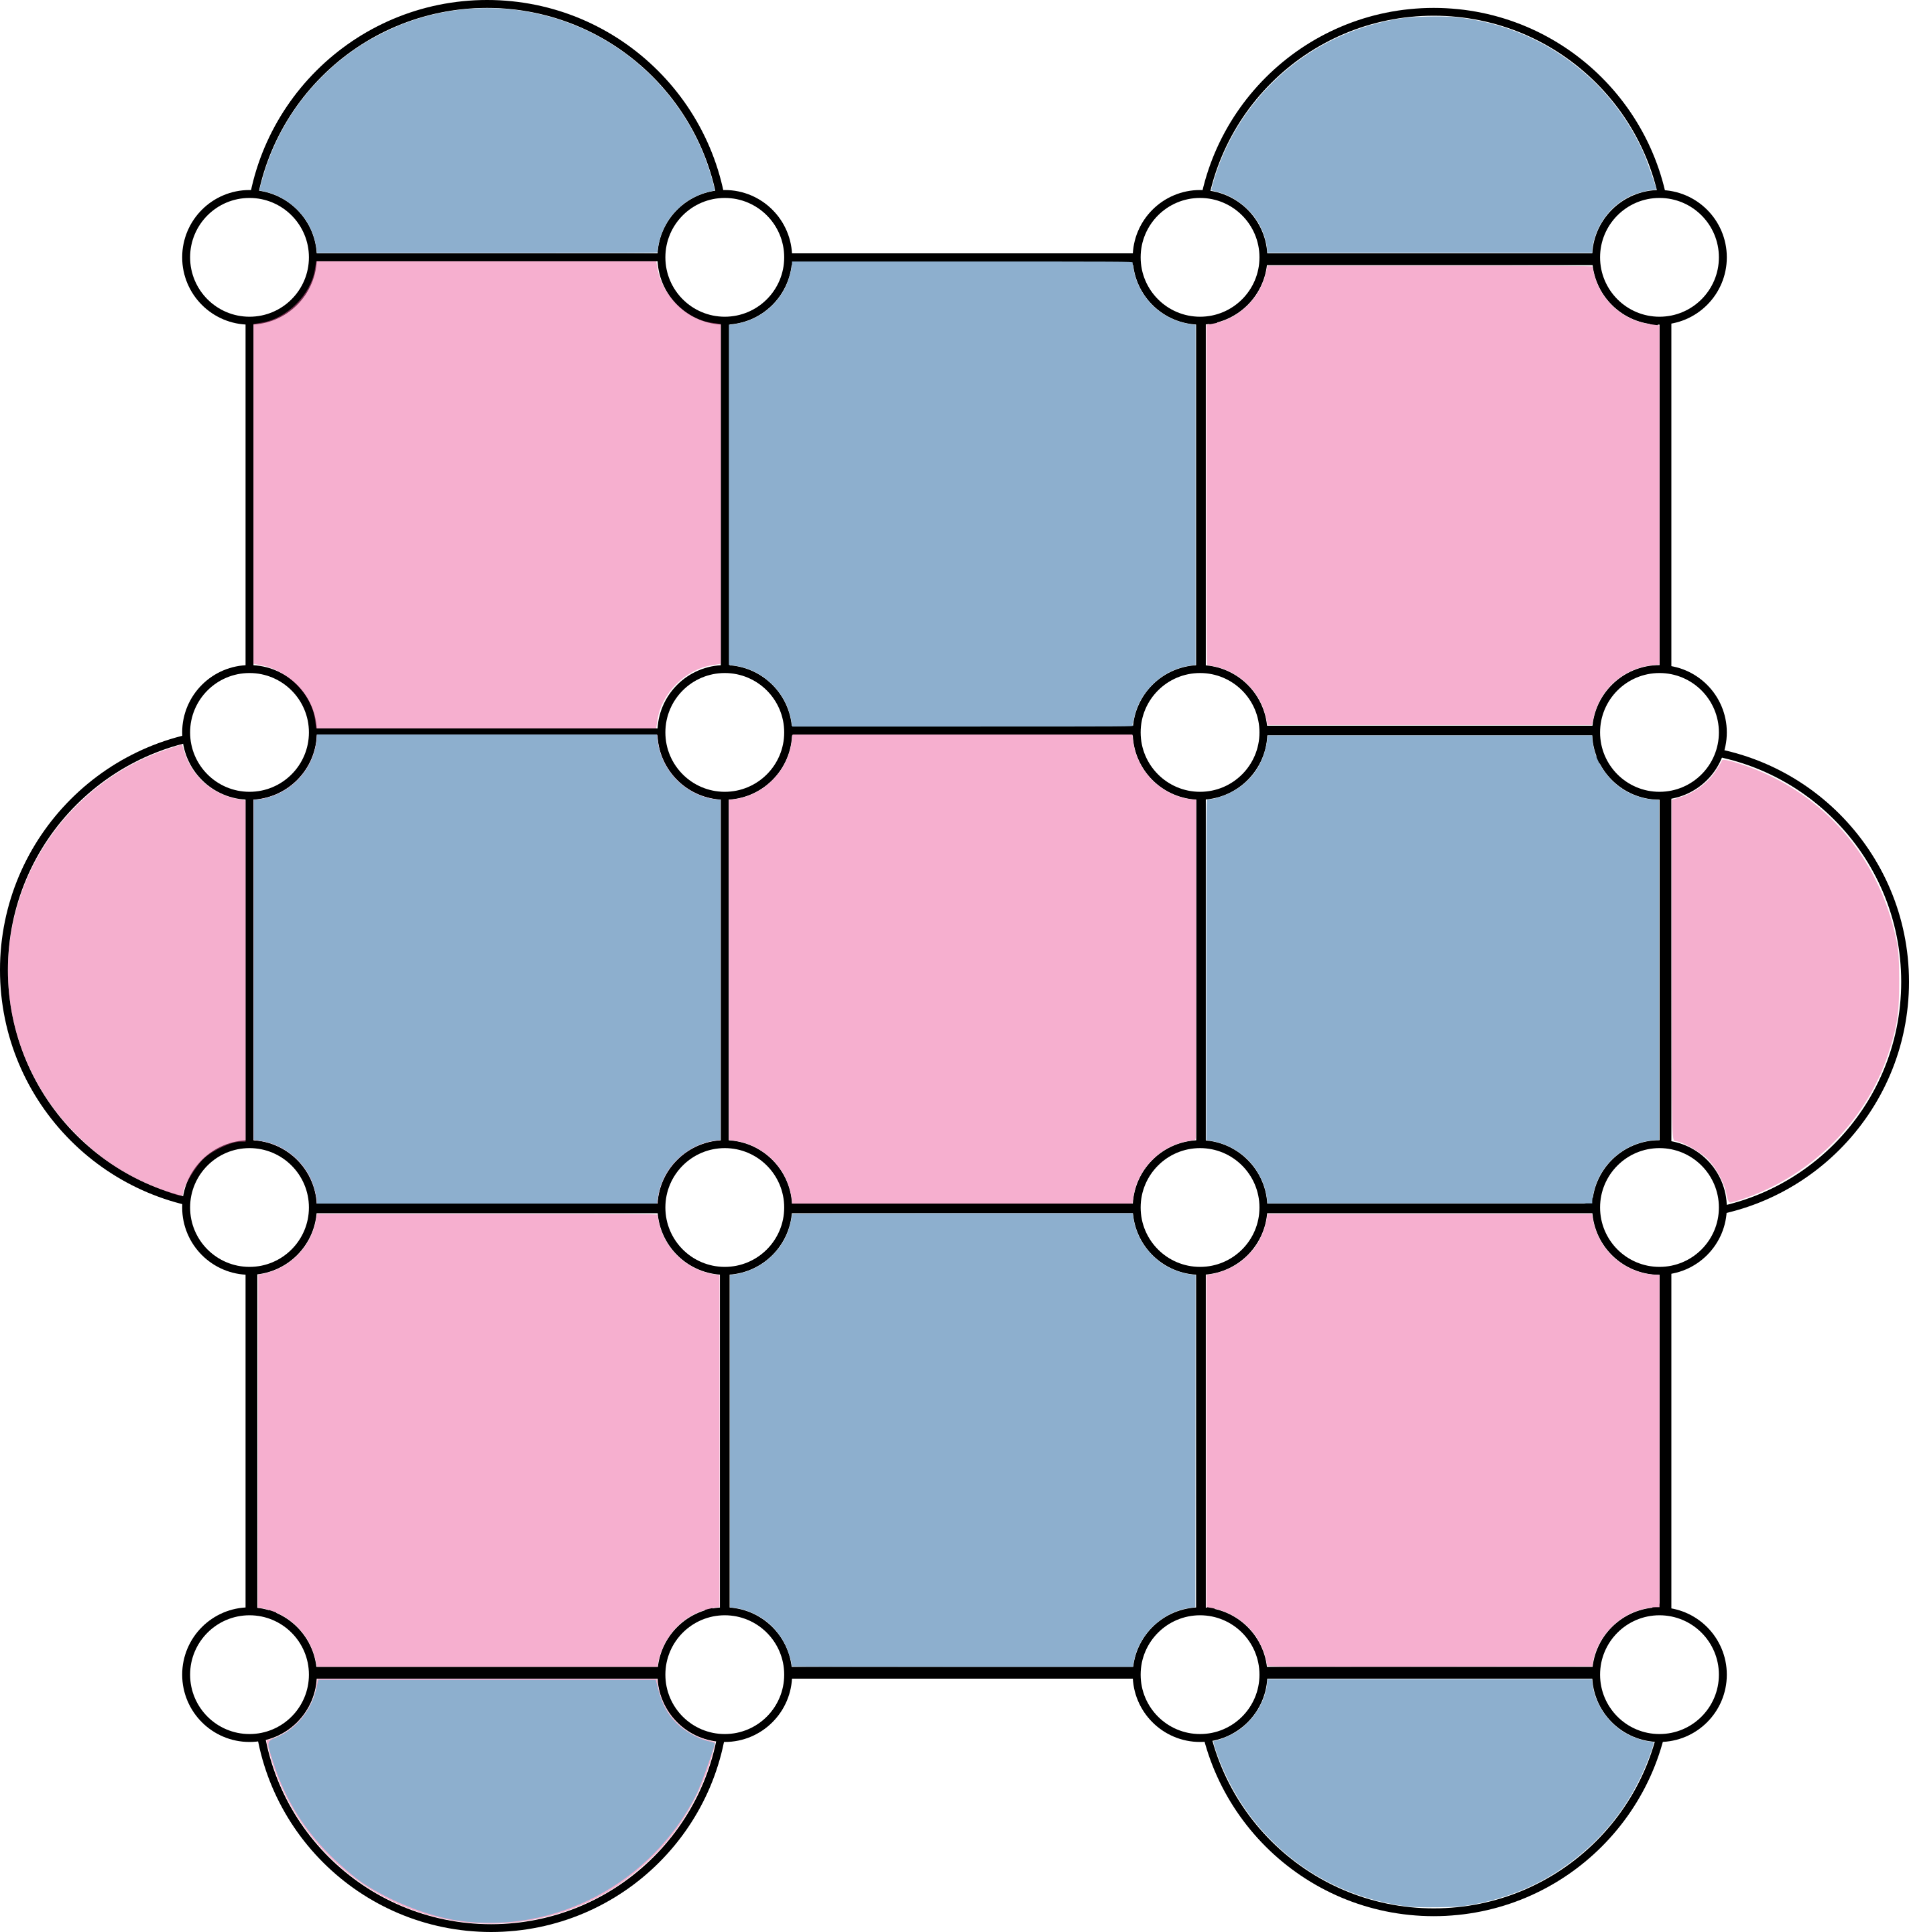
\includegraphics[width=0.55\textwidth]{fig/Rotated_surface_code_d4.png}
	\end{textblock*}
	}
	\only<1-1>{
		\begin{textblock*}{7cm}(8.5cm,2.5cm)
			\begin{itemize}
				\item \citeauthoryear{kitaev_fault-tolerant_2003, bombin_optimal_2007}
				\item Qubits at vertices of the lattice
				\item Encodes 1 logical qubit
			\end{itemize}
		\end{textblock*}
	}
	\only<2-2>{
		\begin{textblock*}{7cm}(8.5cm,2cm)
			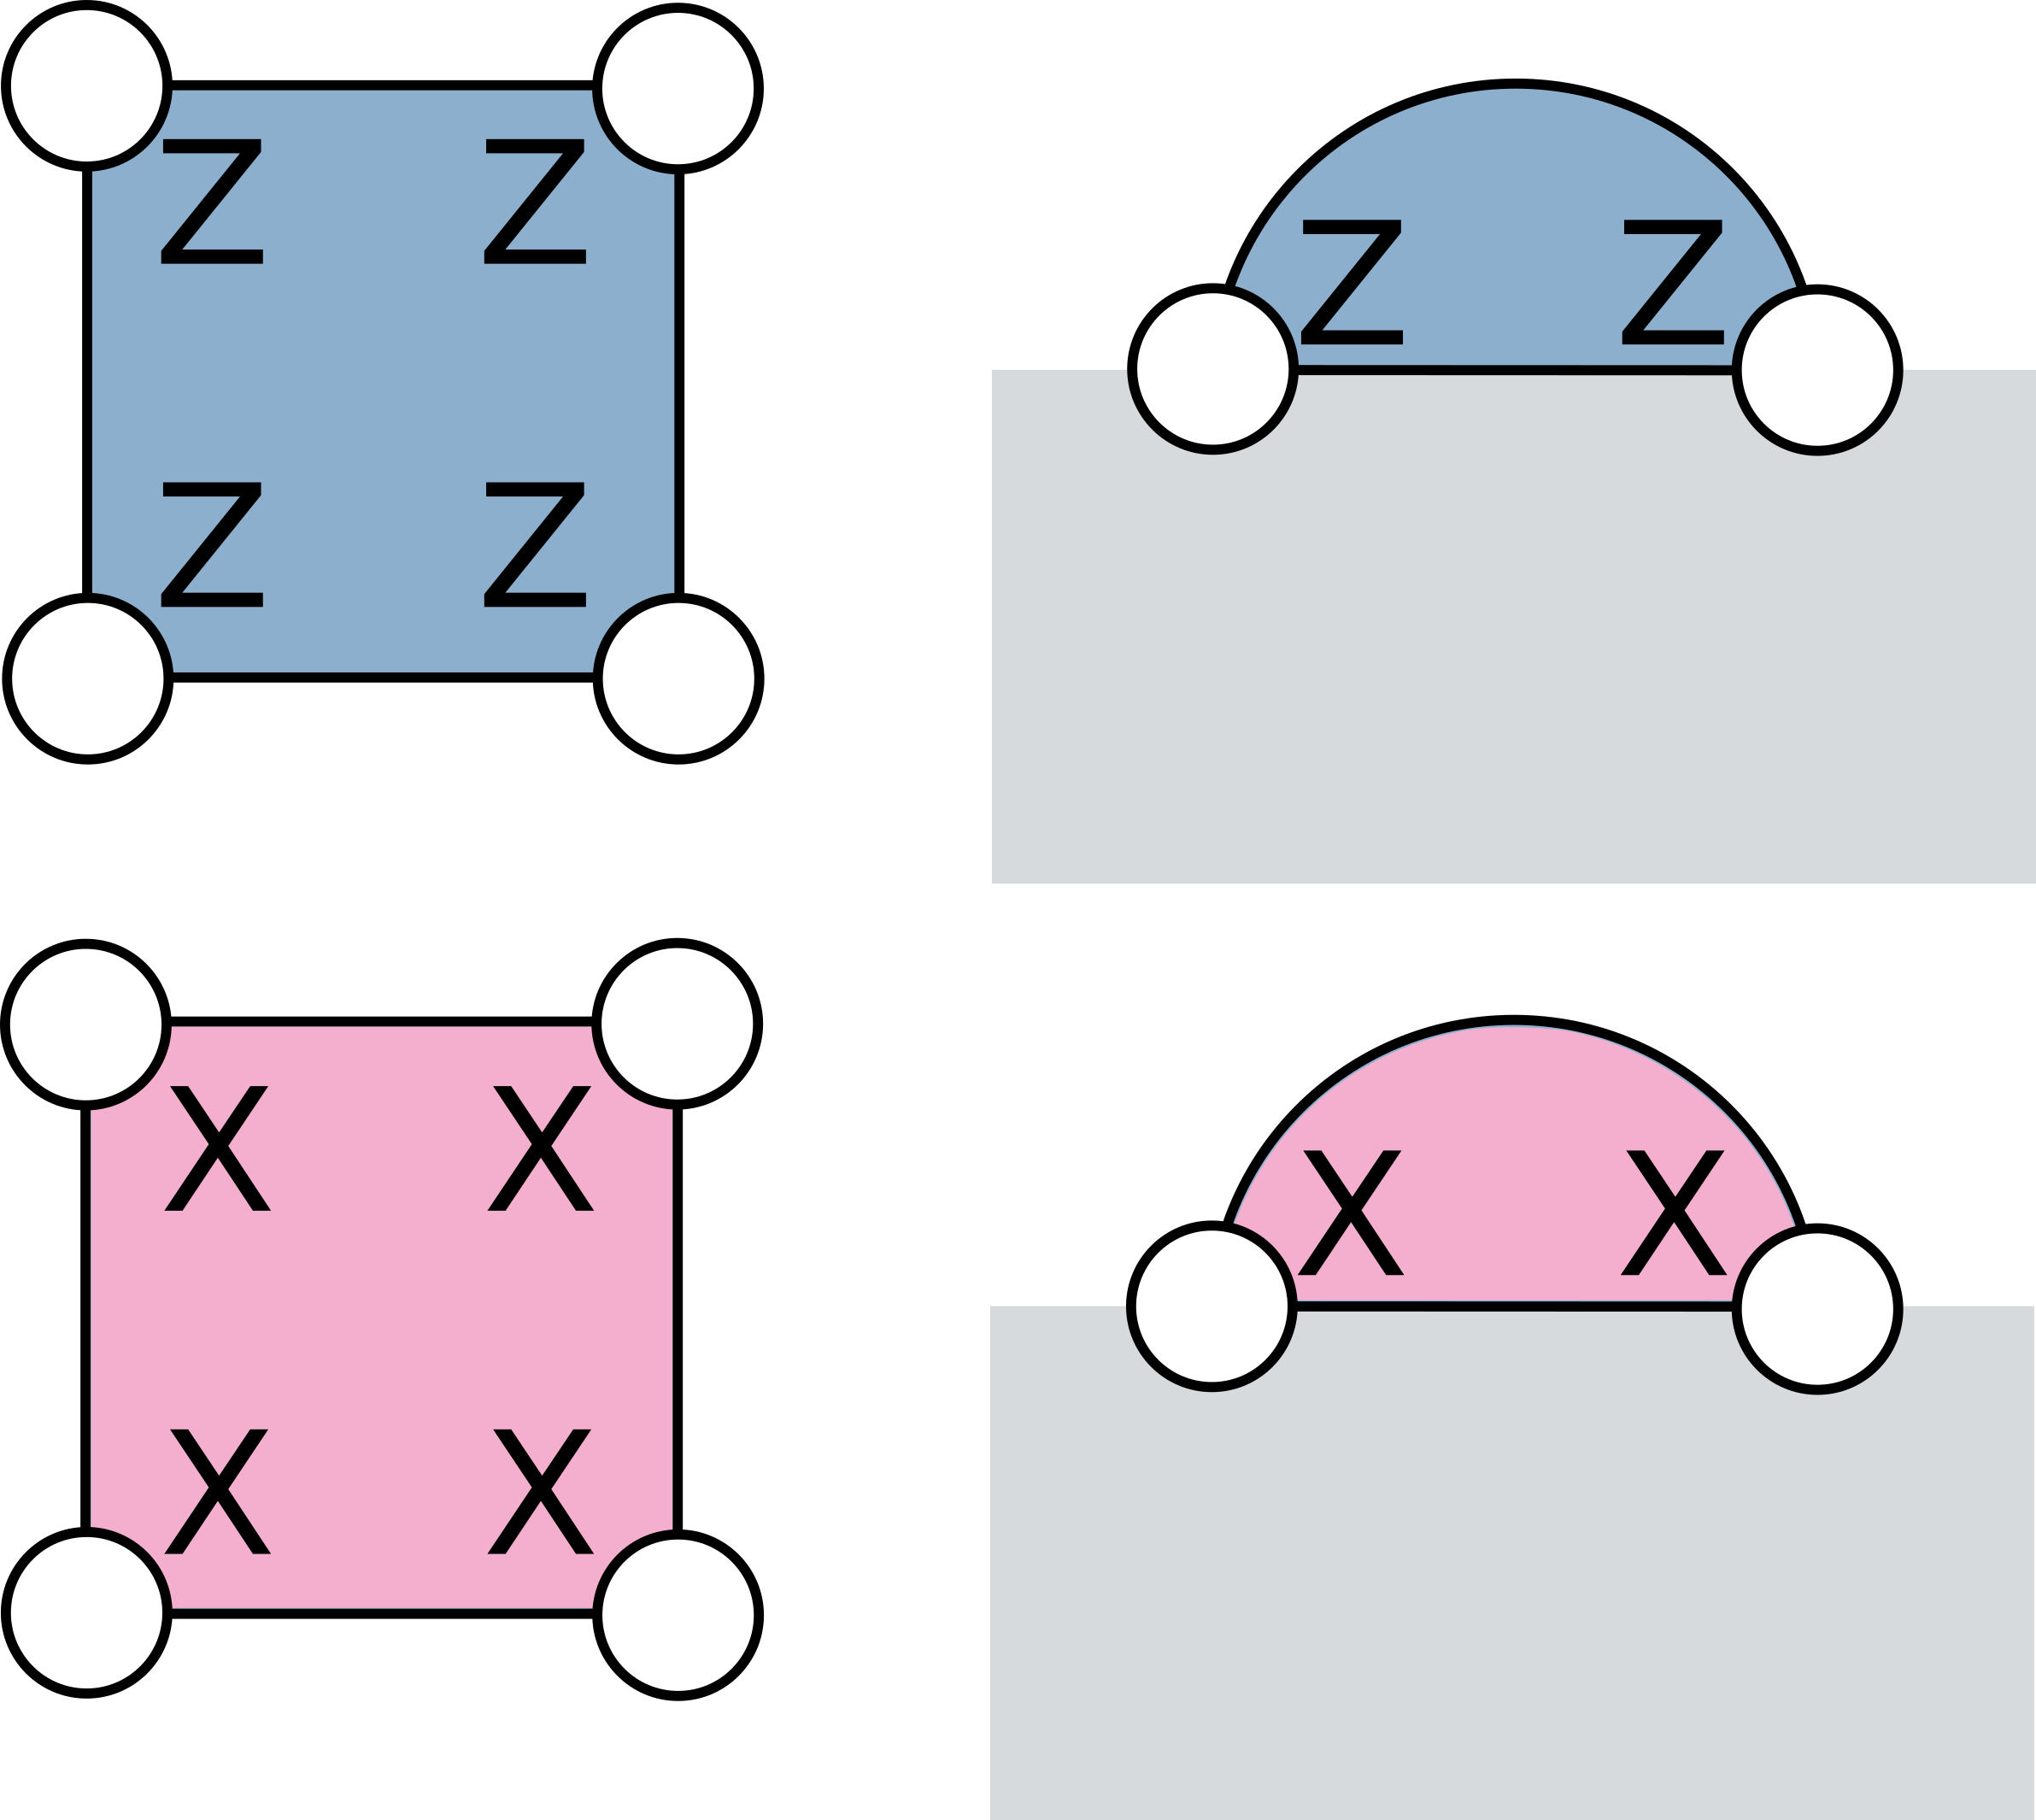
\includegraphics[width=0.55\textwidth]{fig/Syndromes.png}
		\end{textblock*}
		\begin{textblock*}{13cm}(2.5cm,7cm)
			Measurement of stabilizers gives partial error information. \\
		\end{textblock*}
	}
	\only<3->{
		\begin{textblock*}{7cm}(1.5cm,2cm)
			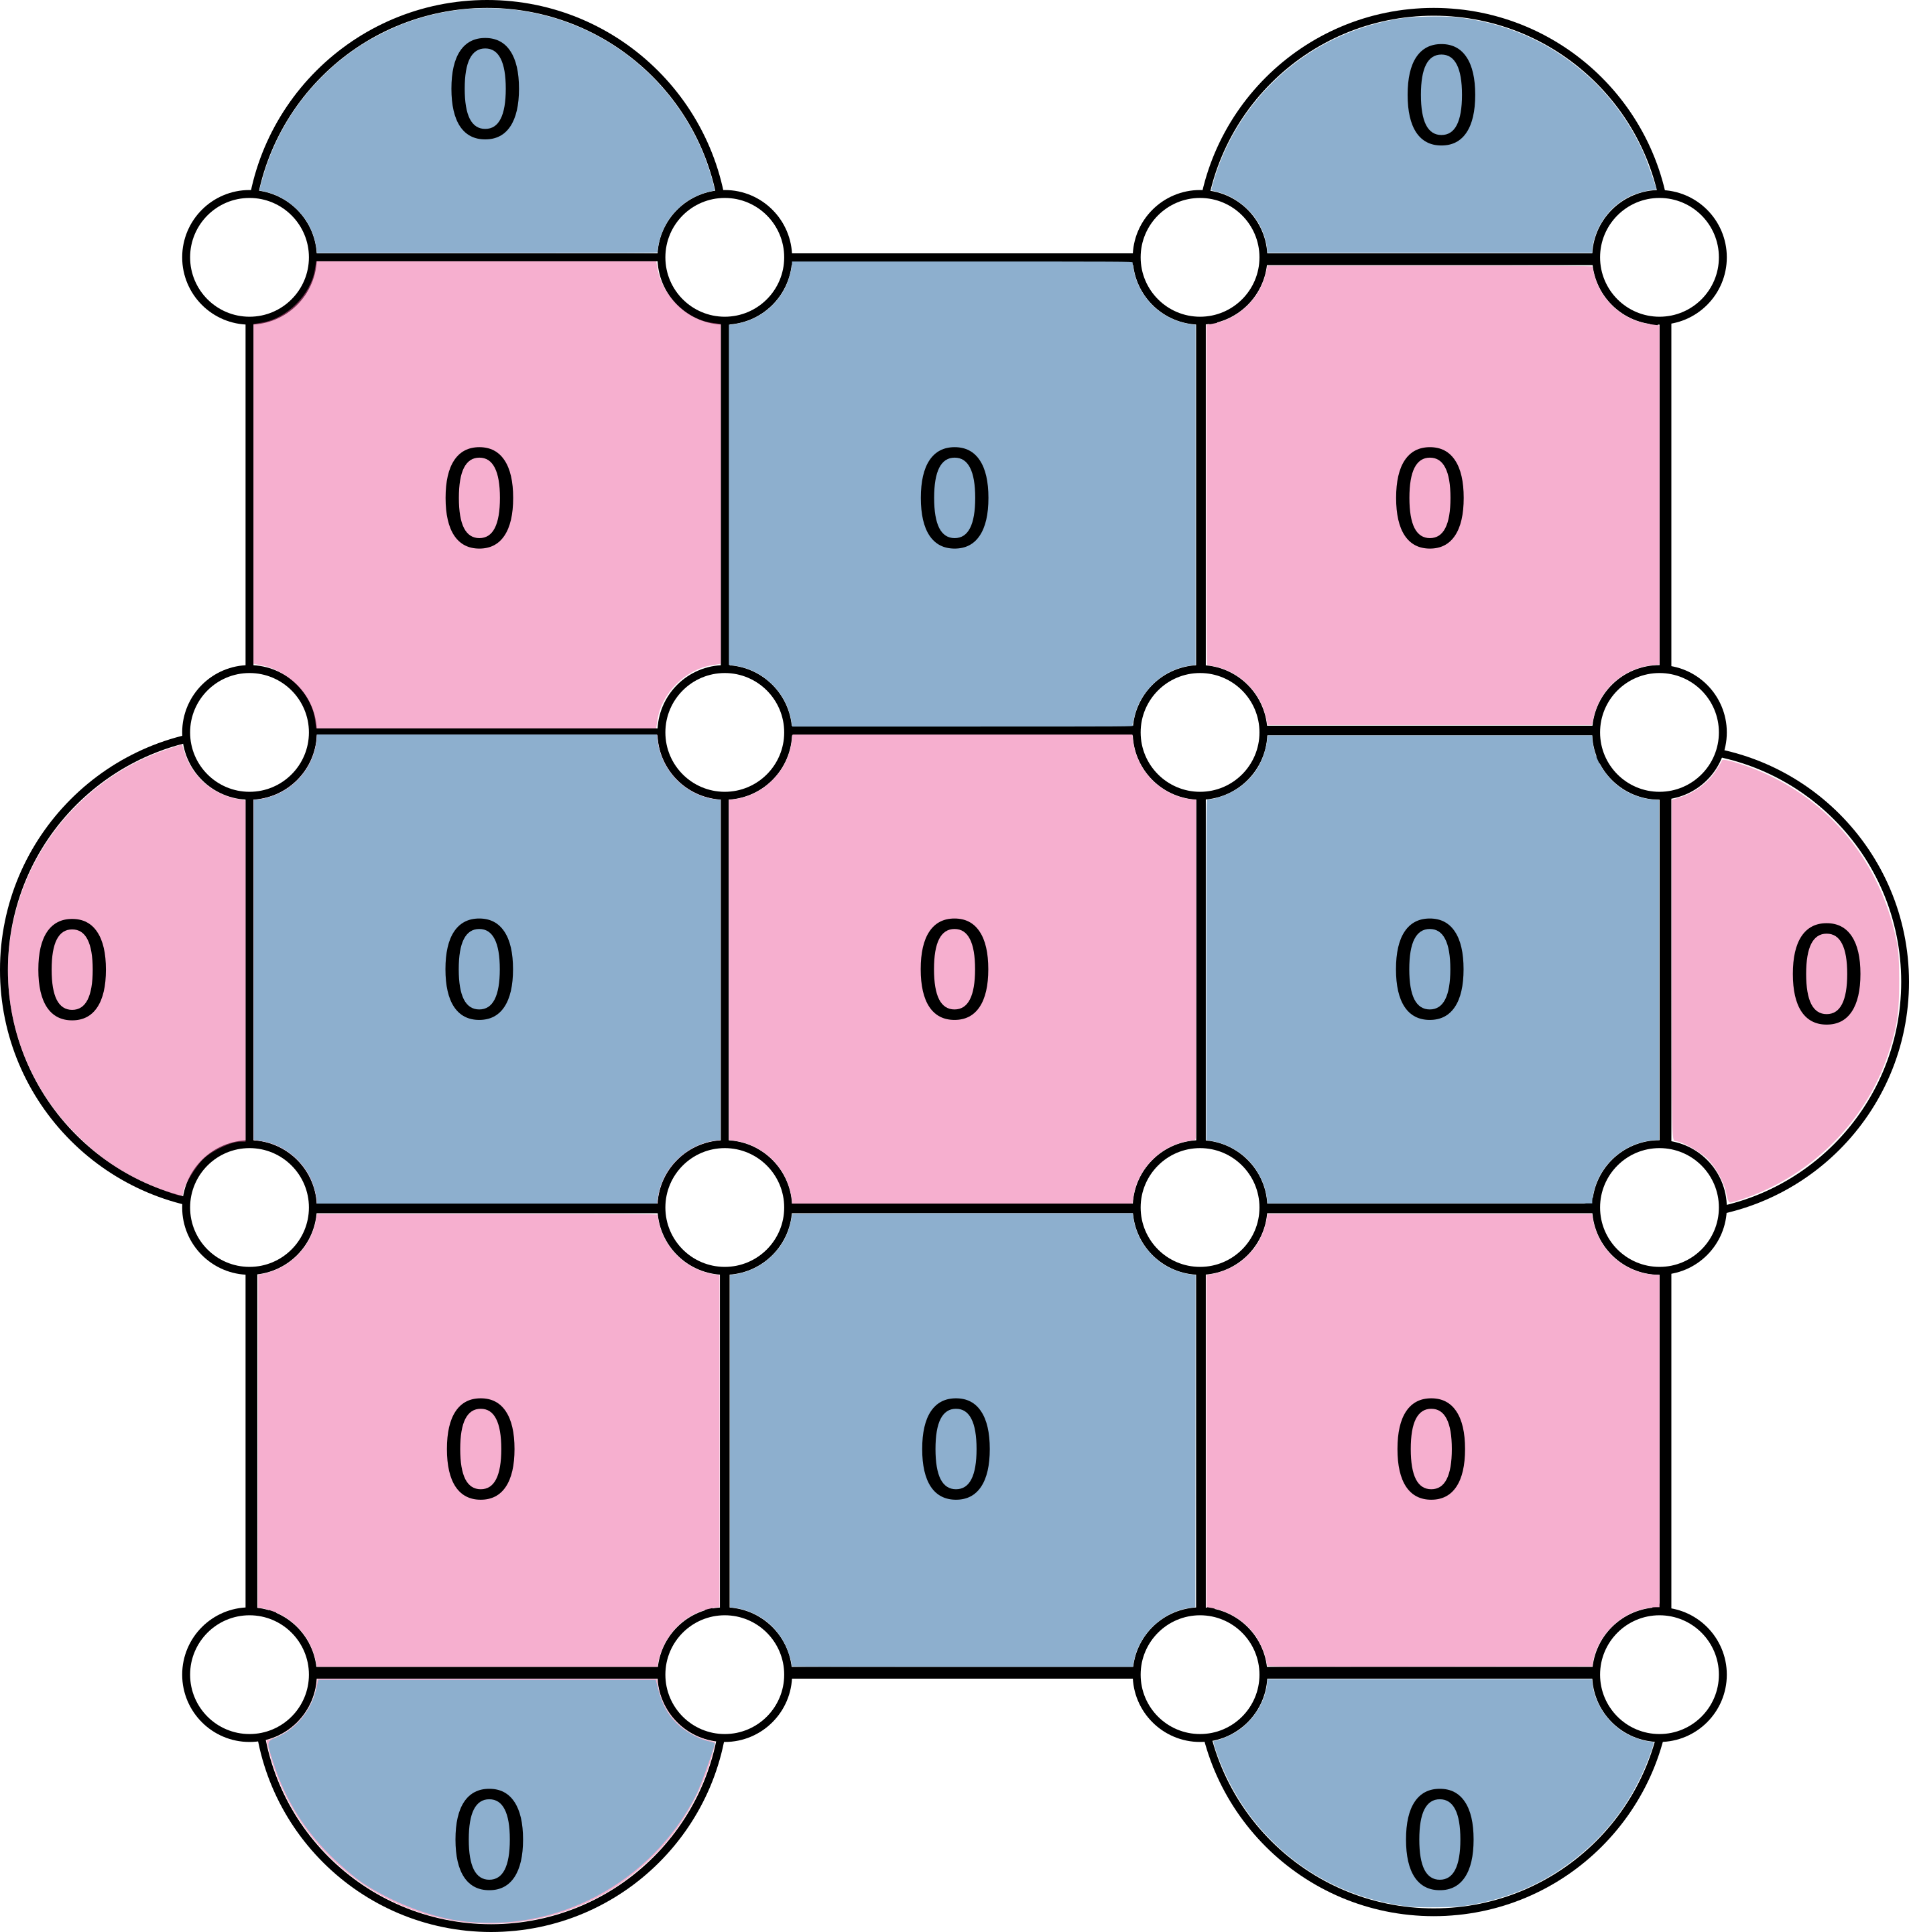
\includegraphics[width=0.55\textwidth]{fig/Rotated_surface_code_d4_error_free.png}
		\end{textblock*}
		\begin{textblock*}{7cm}(8.5cm,2cm)
			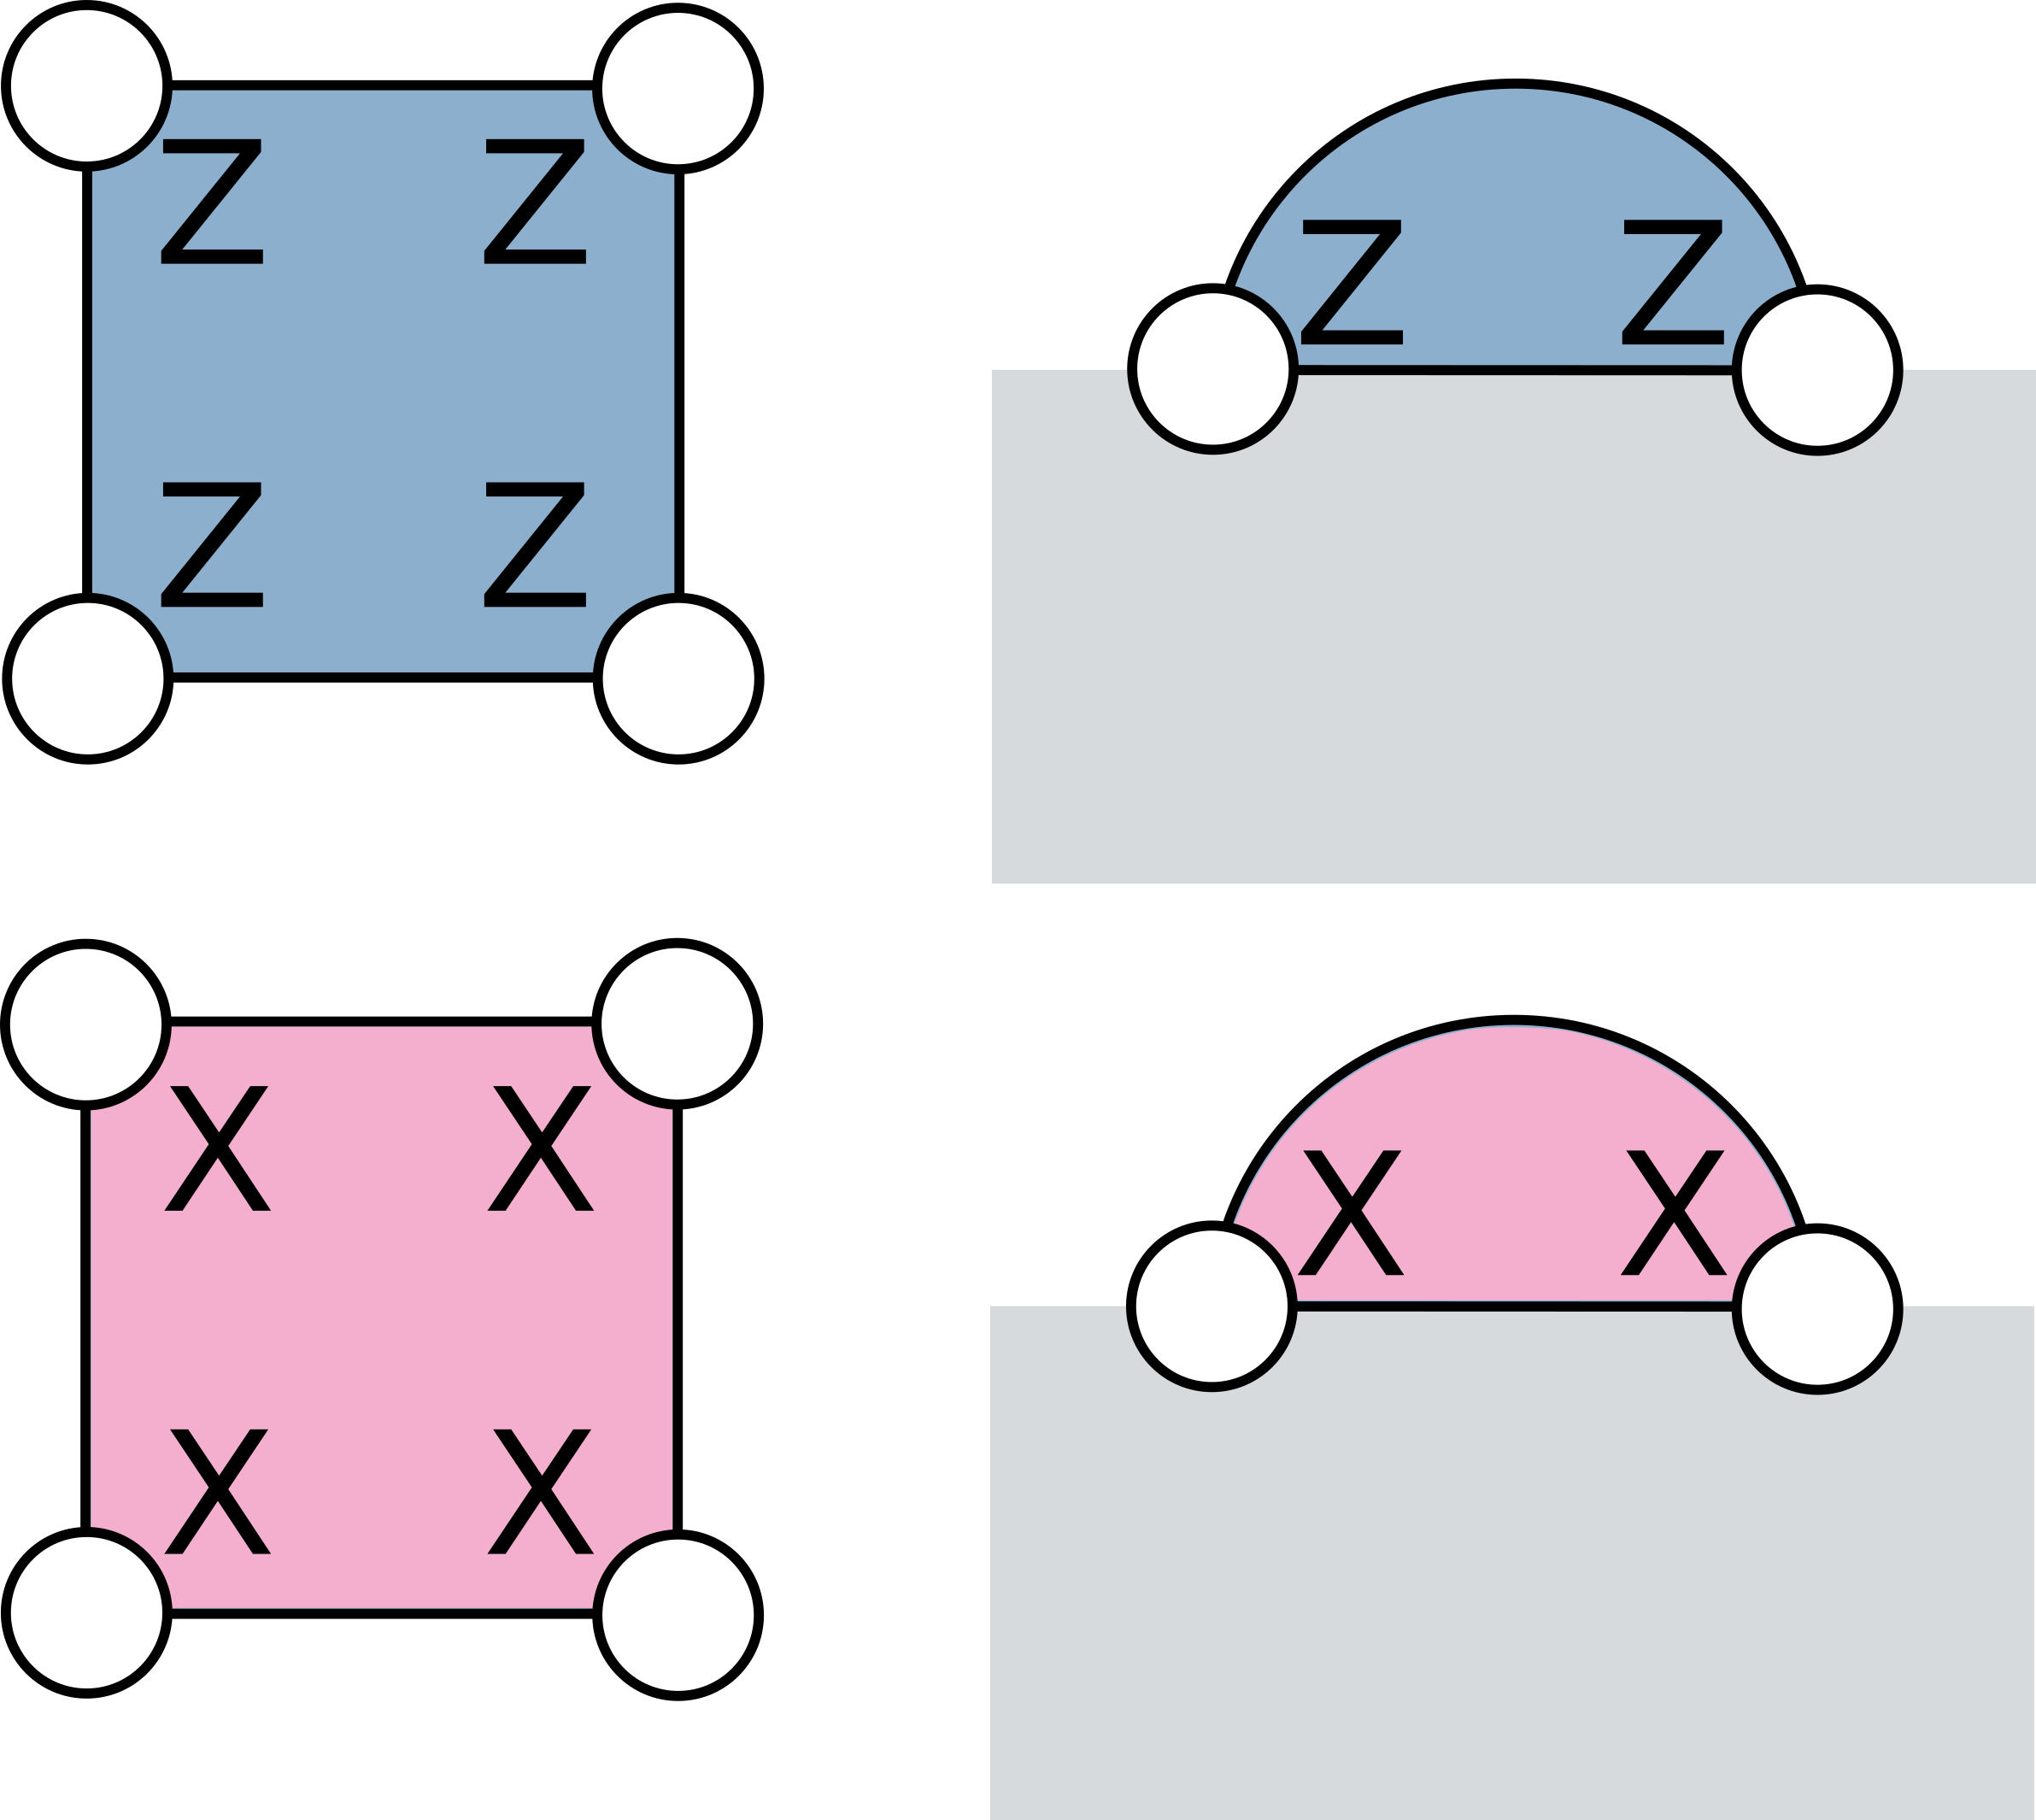
\includegraphics[width=0.55\textwidth]{fig/Syndromes.png}
		\end{textblock*}
		\begin{textblock*}{13cm}(2.5cm,7cm)
			Measurement of stabilizers gives partial error information. \\
			In absence of errors, all stabilizers return $0$. \\
		\end{textblock*}
	}
\end{frame}

\begin{frame}{Example: Surface Code}
	\only<1-1>{
		\begin{textblock*}{7cm}(1.5cm,2cm)
			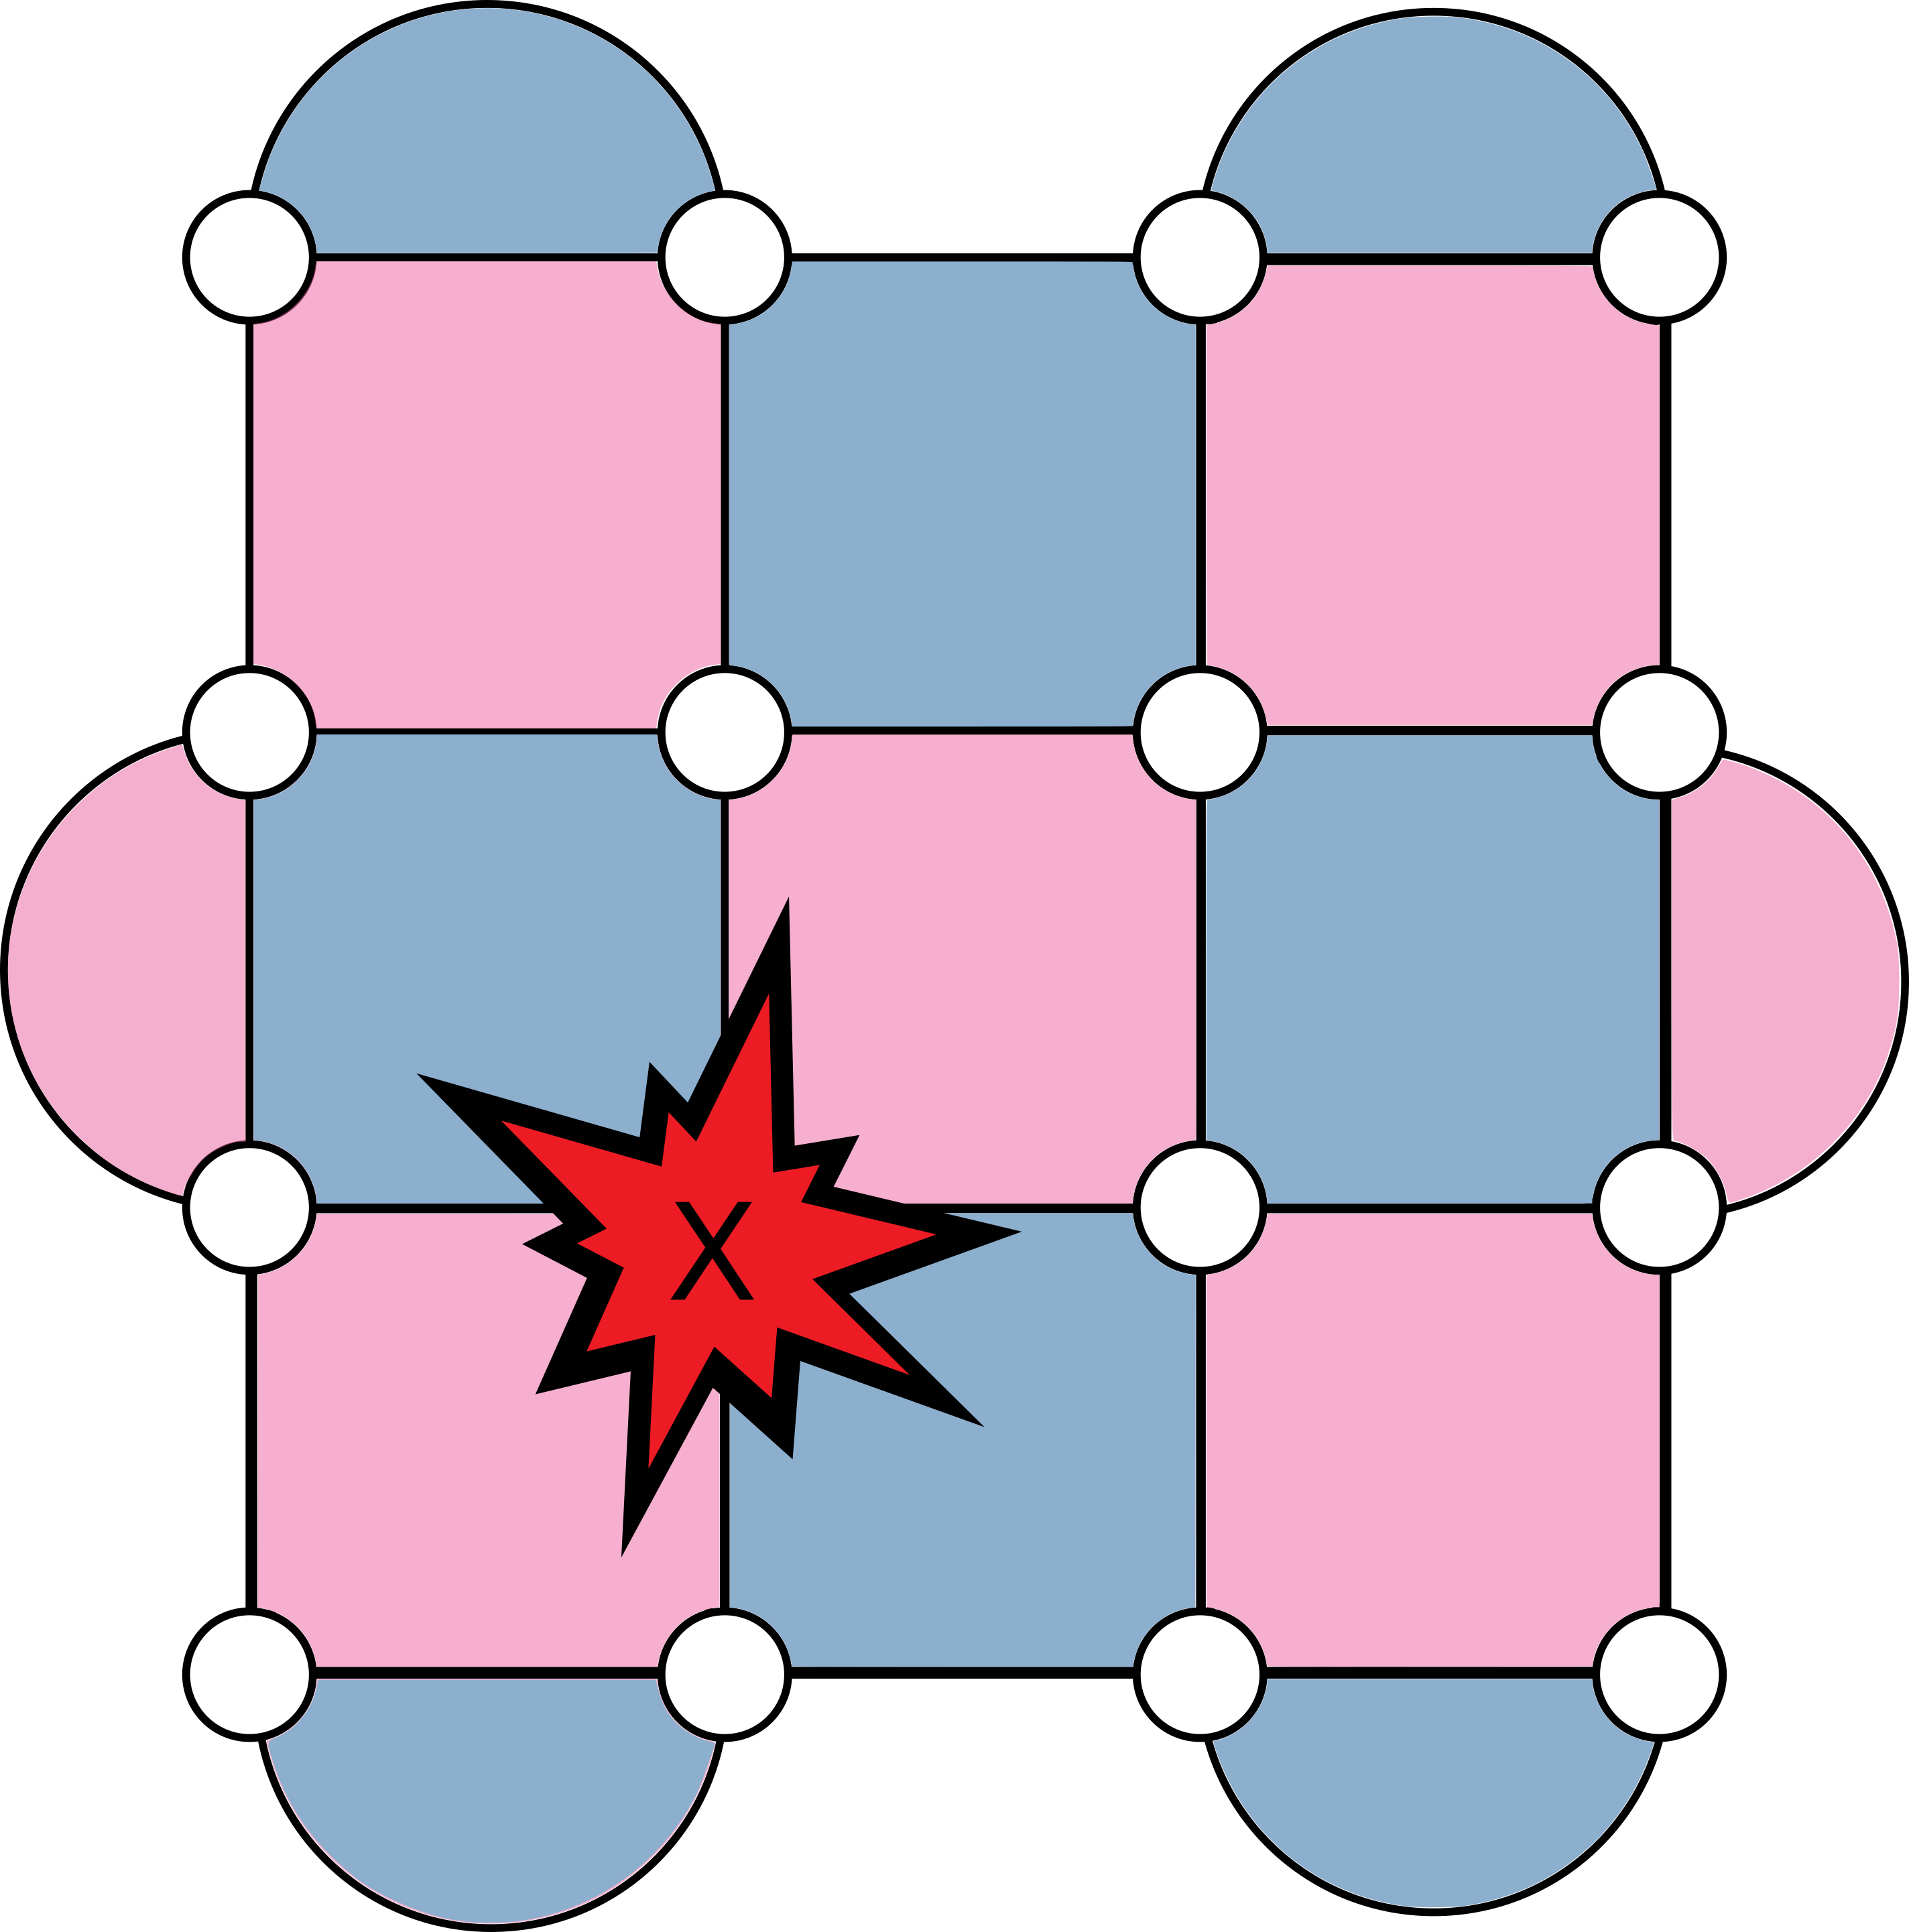
\includegraphics[width=0.55\textwidth]{fig/Rotated_surface_code_d4_error_appears.png}
		\end{textblock*}
		\begin{textblock*}{9cm}(6.5cm,3.5cm)
			Bitflip error appears
		\end{textblock*}
	}
	\pause
	\only<2-2>{
		\begin{textblock*}{7cm}(1.5cm,2cm)
			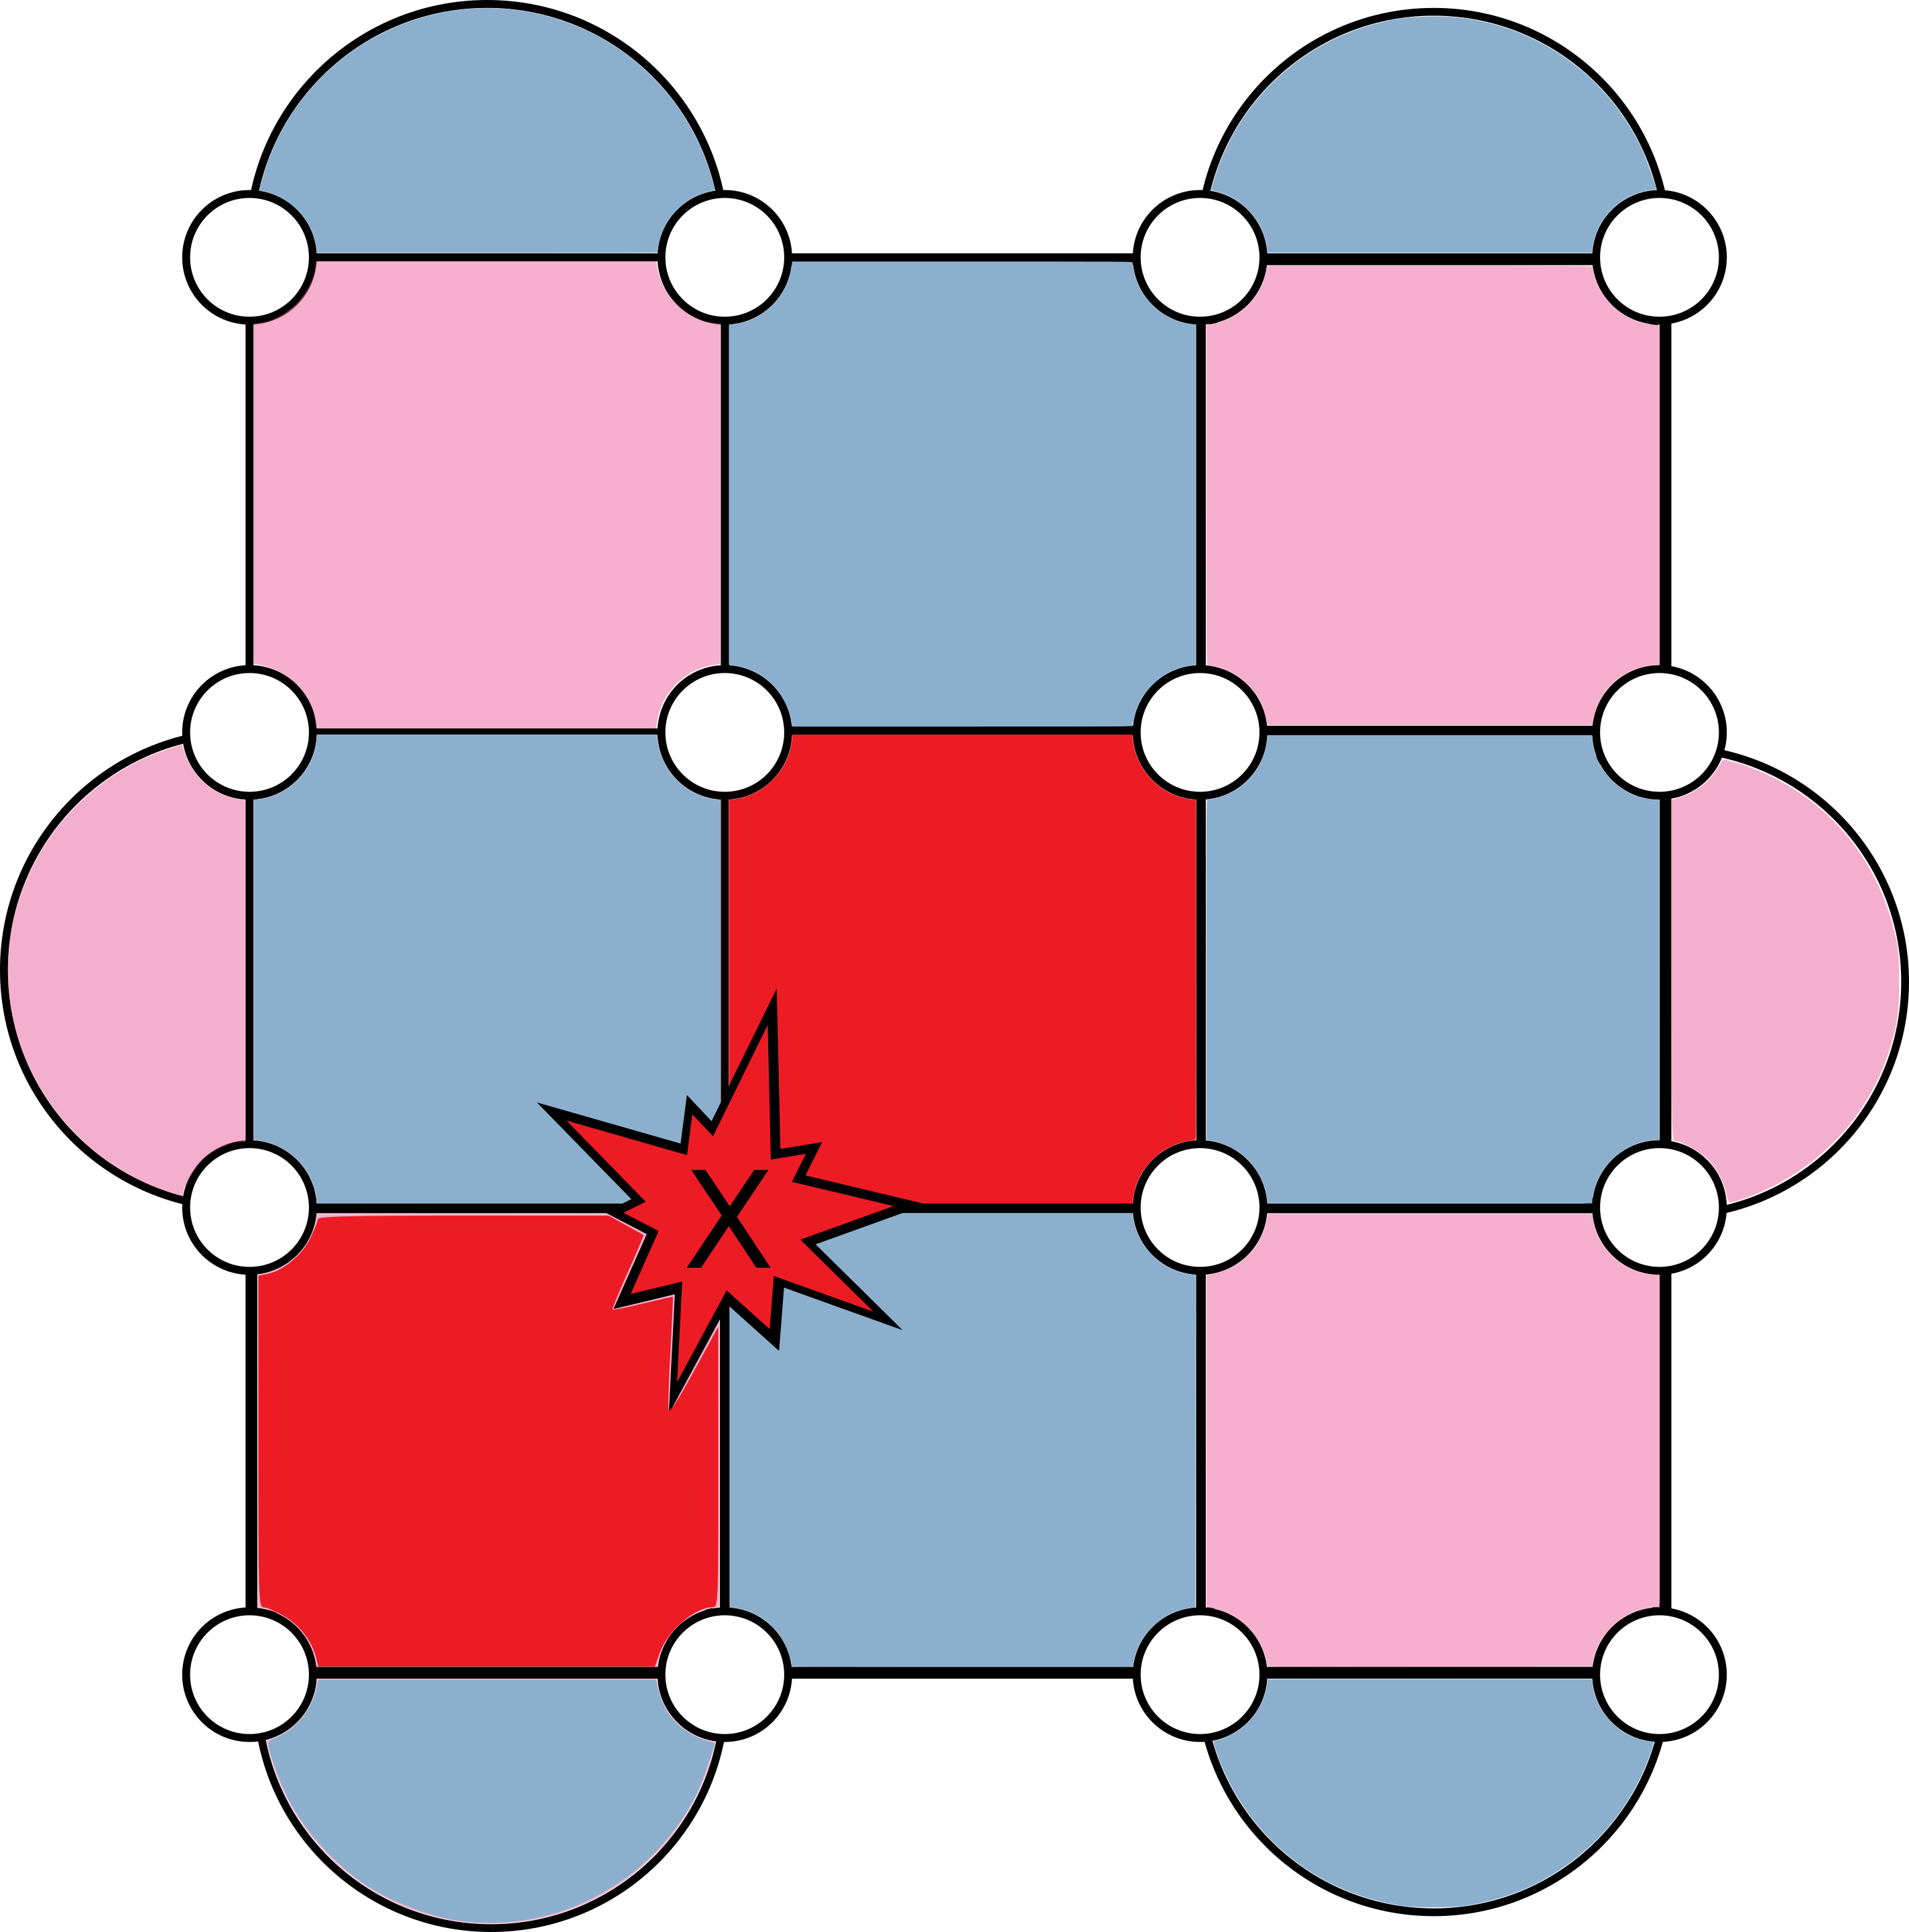
\includegraphics[width=0.55\textwidth]{fig/Rotated_surface_code_d4_syndromes.png}
		\end{textblock*}
		\begin{textblock*}{9cm}(6.5cm,3.5cm)
			Bitflip error appears $\rightarrow$ Pair of Z-stabilizers return error information
		\end{textblock*}
	}
\end{frame}

\begin{frame}{Example: Surface Code Decoder}
	\only<1-1>{
		\begin{textblock*}{7cm}(1.5cm,2cm)
			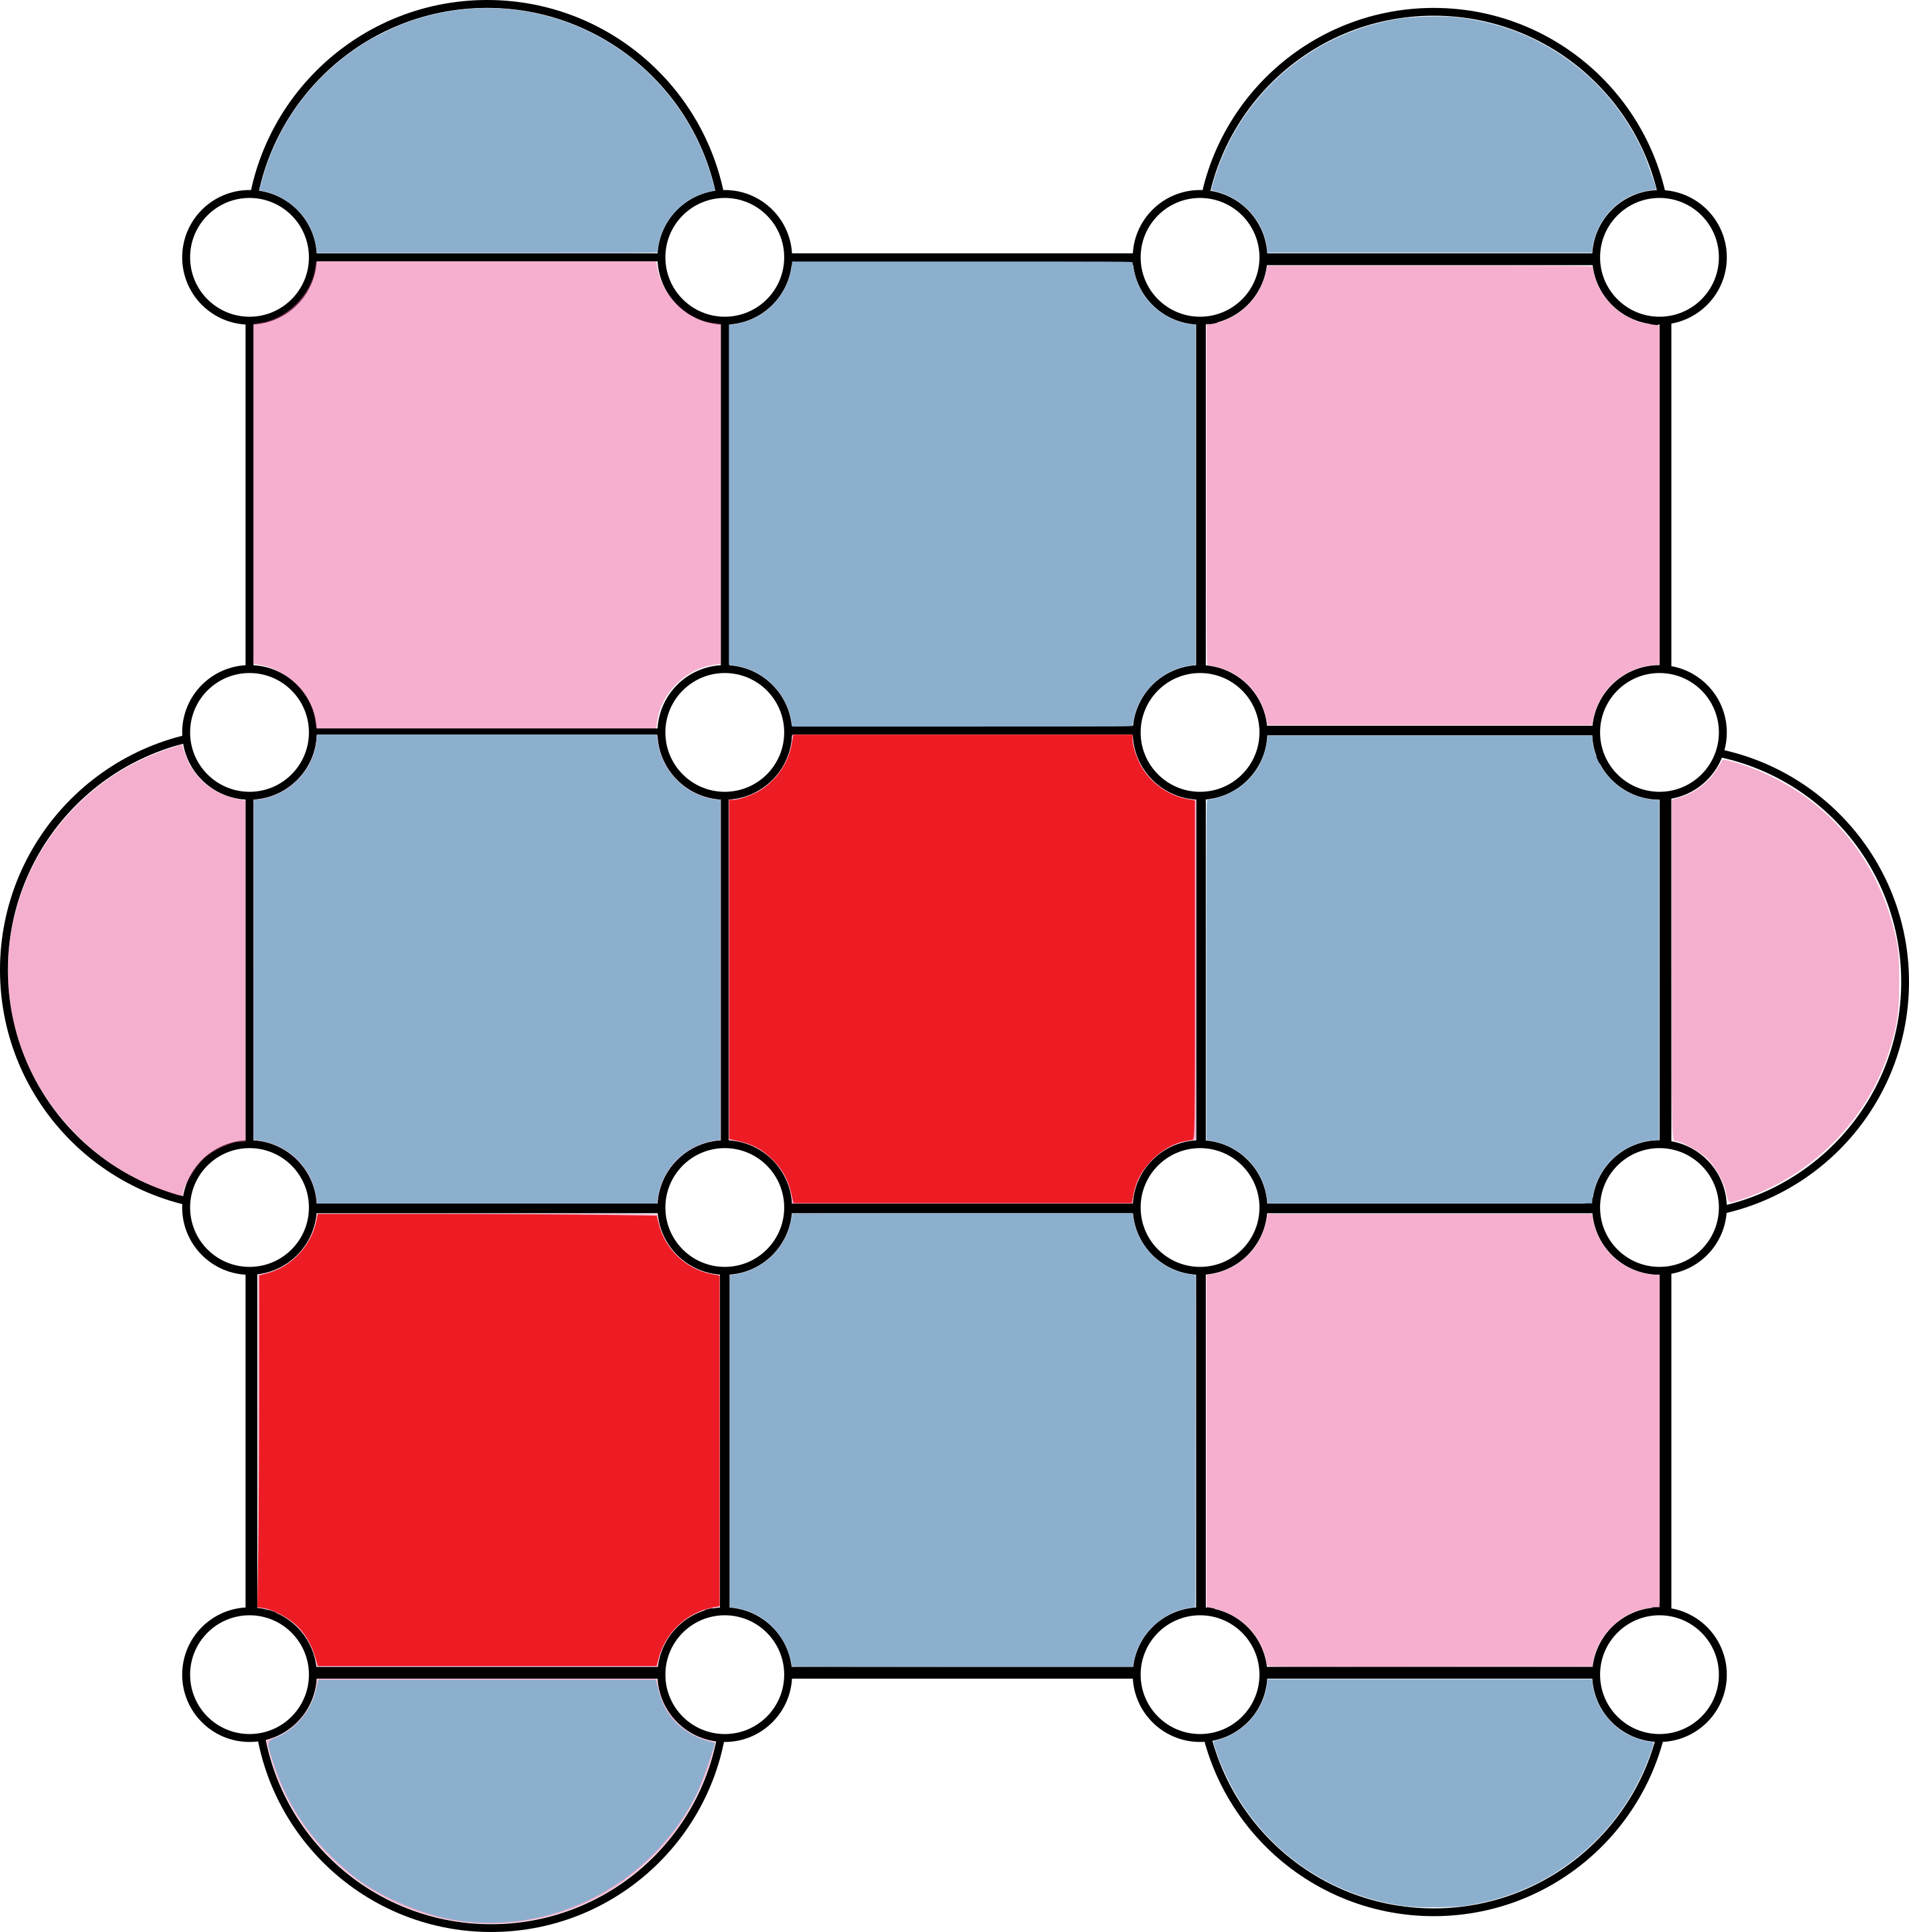
\includegraphics[width=0.55\textwidth]{fig/Rotated_surface_code_d4_only_syndromes.png}
		\end{textblock*}
		\begin{textblock*}{9cm}(6.5cm,3.5cm)
			\textbf{Maximum Probability Decoder:}\\
			Select most probable error consistent with the partial error information
		\end{textblock*}
	}
	\only<2-2>{
		\begin{textblock*}{7cm}(1.5cm,2cm)
			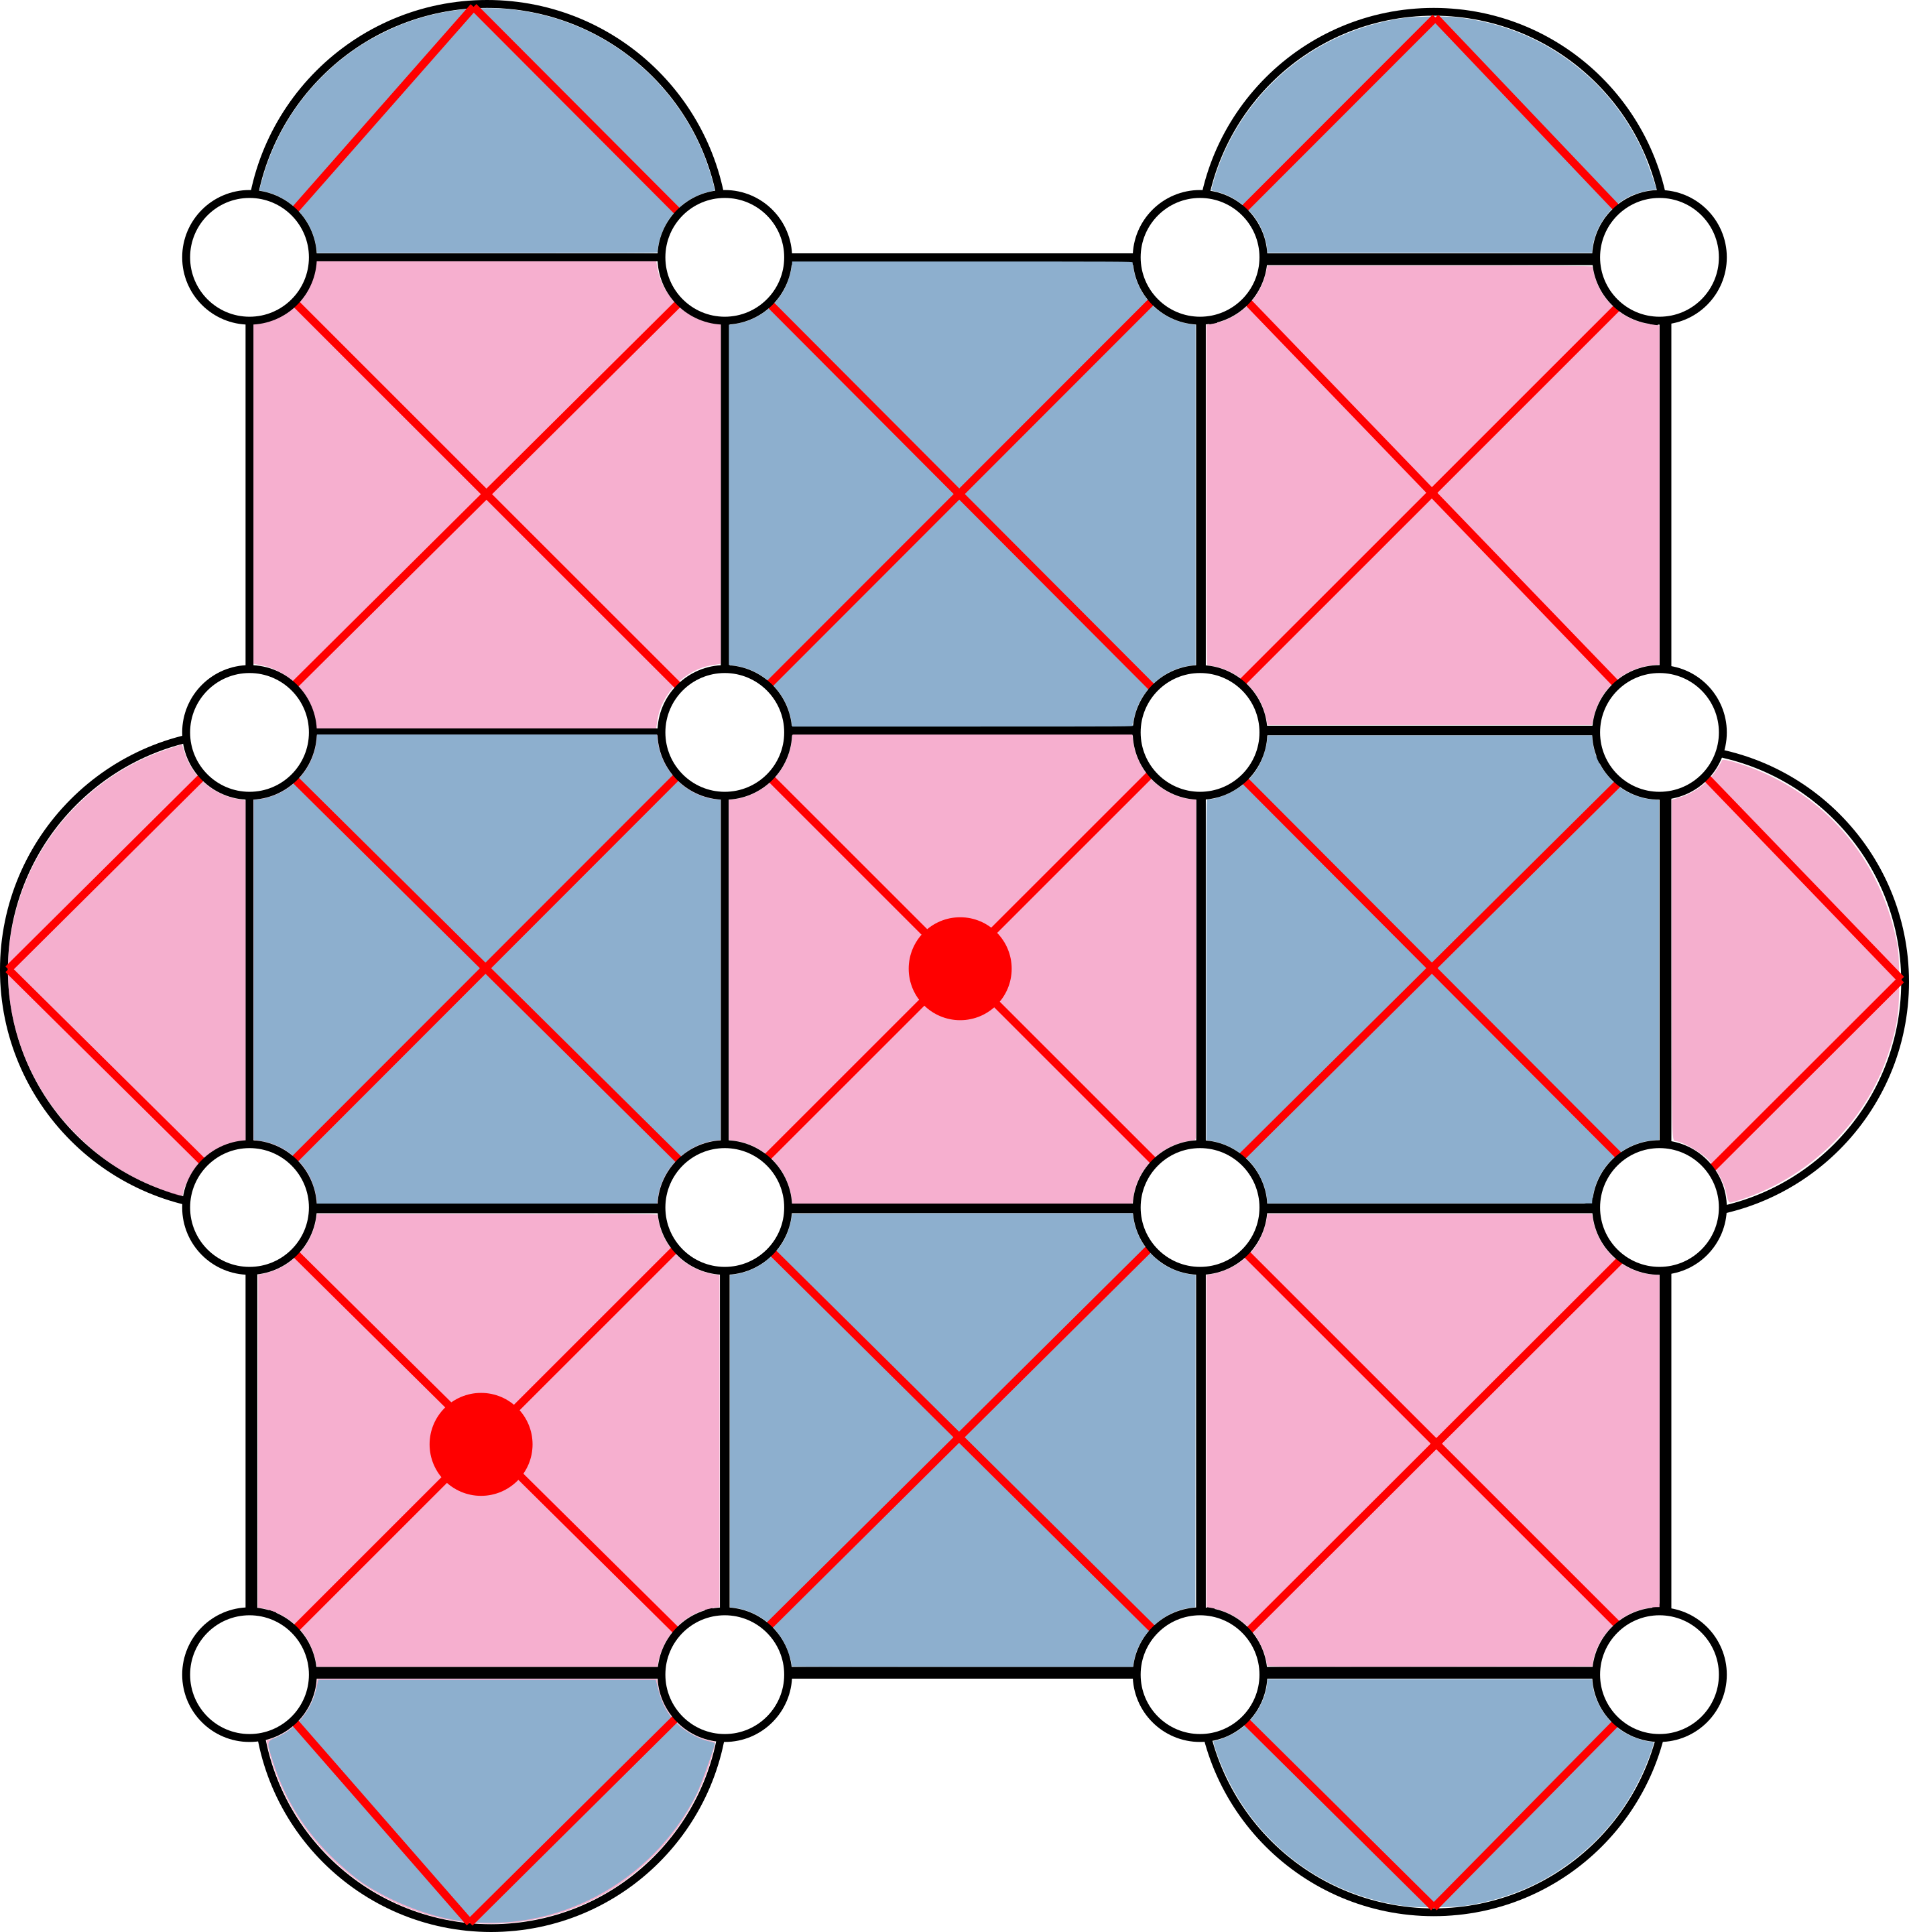
\includegraphics[width=0.55\textwidth]{fig/Rotated_surface_code_d4_decoder_graph.png}
		\end{textblock*}
		\begin{textblock*}{10cm}(6cm,3.5cm)
			\textbf{Maximum Probability/Minimum Weight Perfect Matching Decoder~\citeauthoryear{edmonds_paths_1965}:}\\
			Select lowest weight error on decoder graph consistent with the partial error information \\
		\end{textblock*}
	}
	\only<3-3>{
		\begin{textblock*}{7cm}(1.5cm,2cm)
			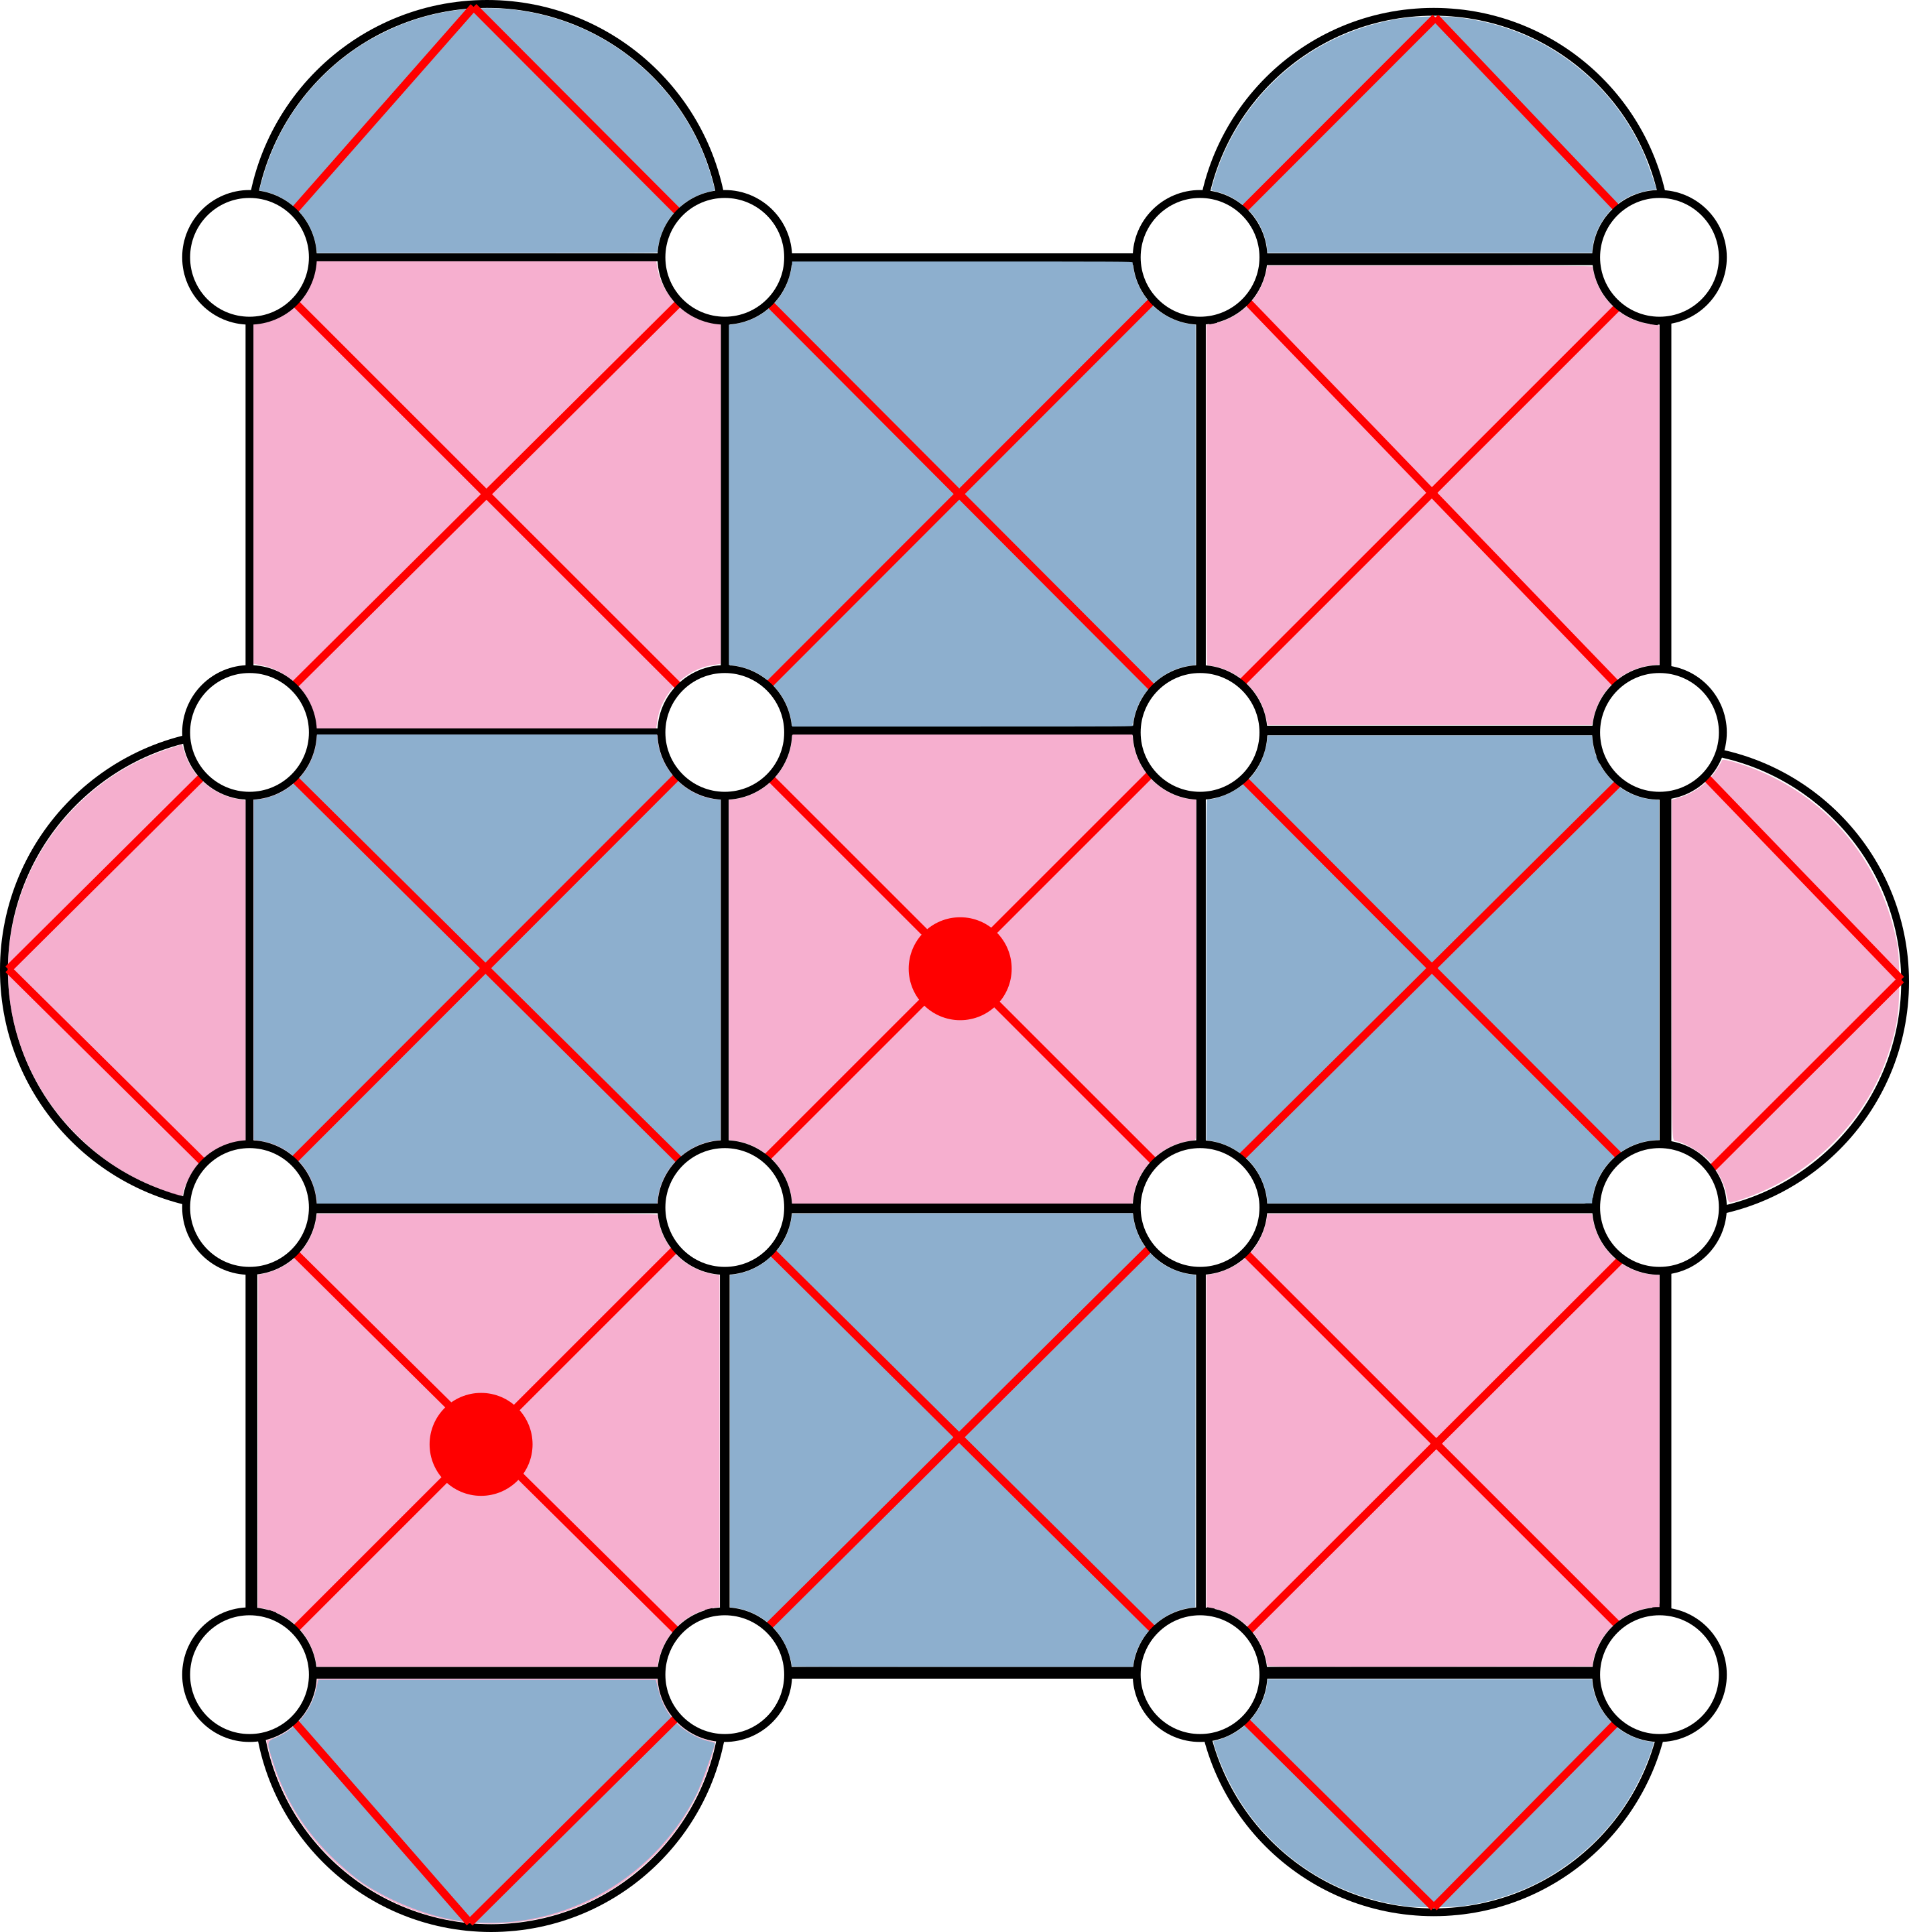
\includegraphics[width=0.55\textwidth]{fig/Rotated_surface_code_d4_decoder_graph.png}
		\end{textblock*}
		\begin{textblock*}{9cm}(6cm,3.5cm)
			\textbf{Maximum Probability/Minimum Weight Perfect Matching Decoder~\citeauthoryear{edmonds_paths_1965}:}\\
			Select lowest weight error on decoder graph consistent with the partial error information \\
			\vspace{0.5cm}
			Sparse blossom implementation: Real time decoding $0.1\%$ depolarising noise on distance-17 surface code \citeauthoryear{higgott_sparse_2025}
		\end{textblock*}
	}
	\only<4-4>{
		\begin{textblock*}{7cm}(1.5cm,2cm)
			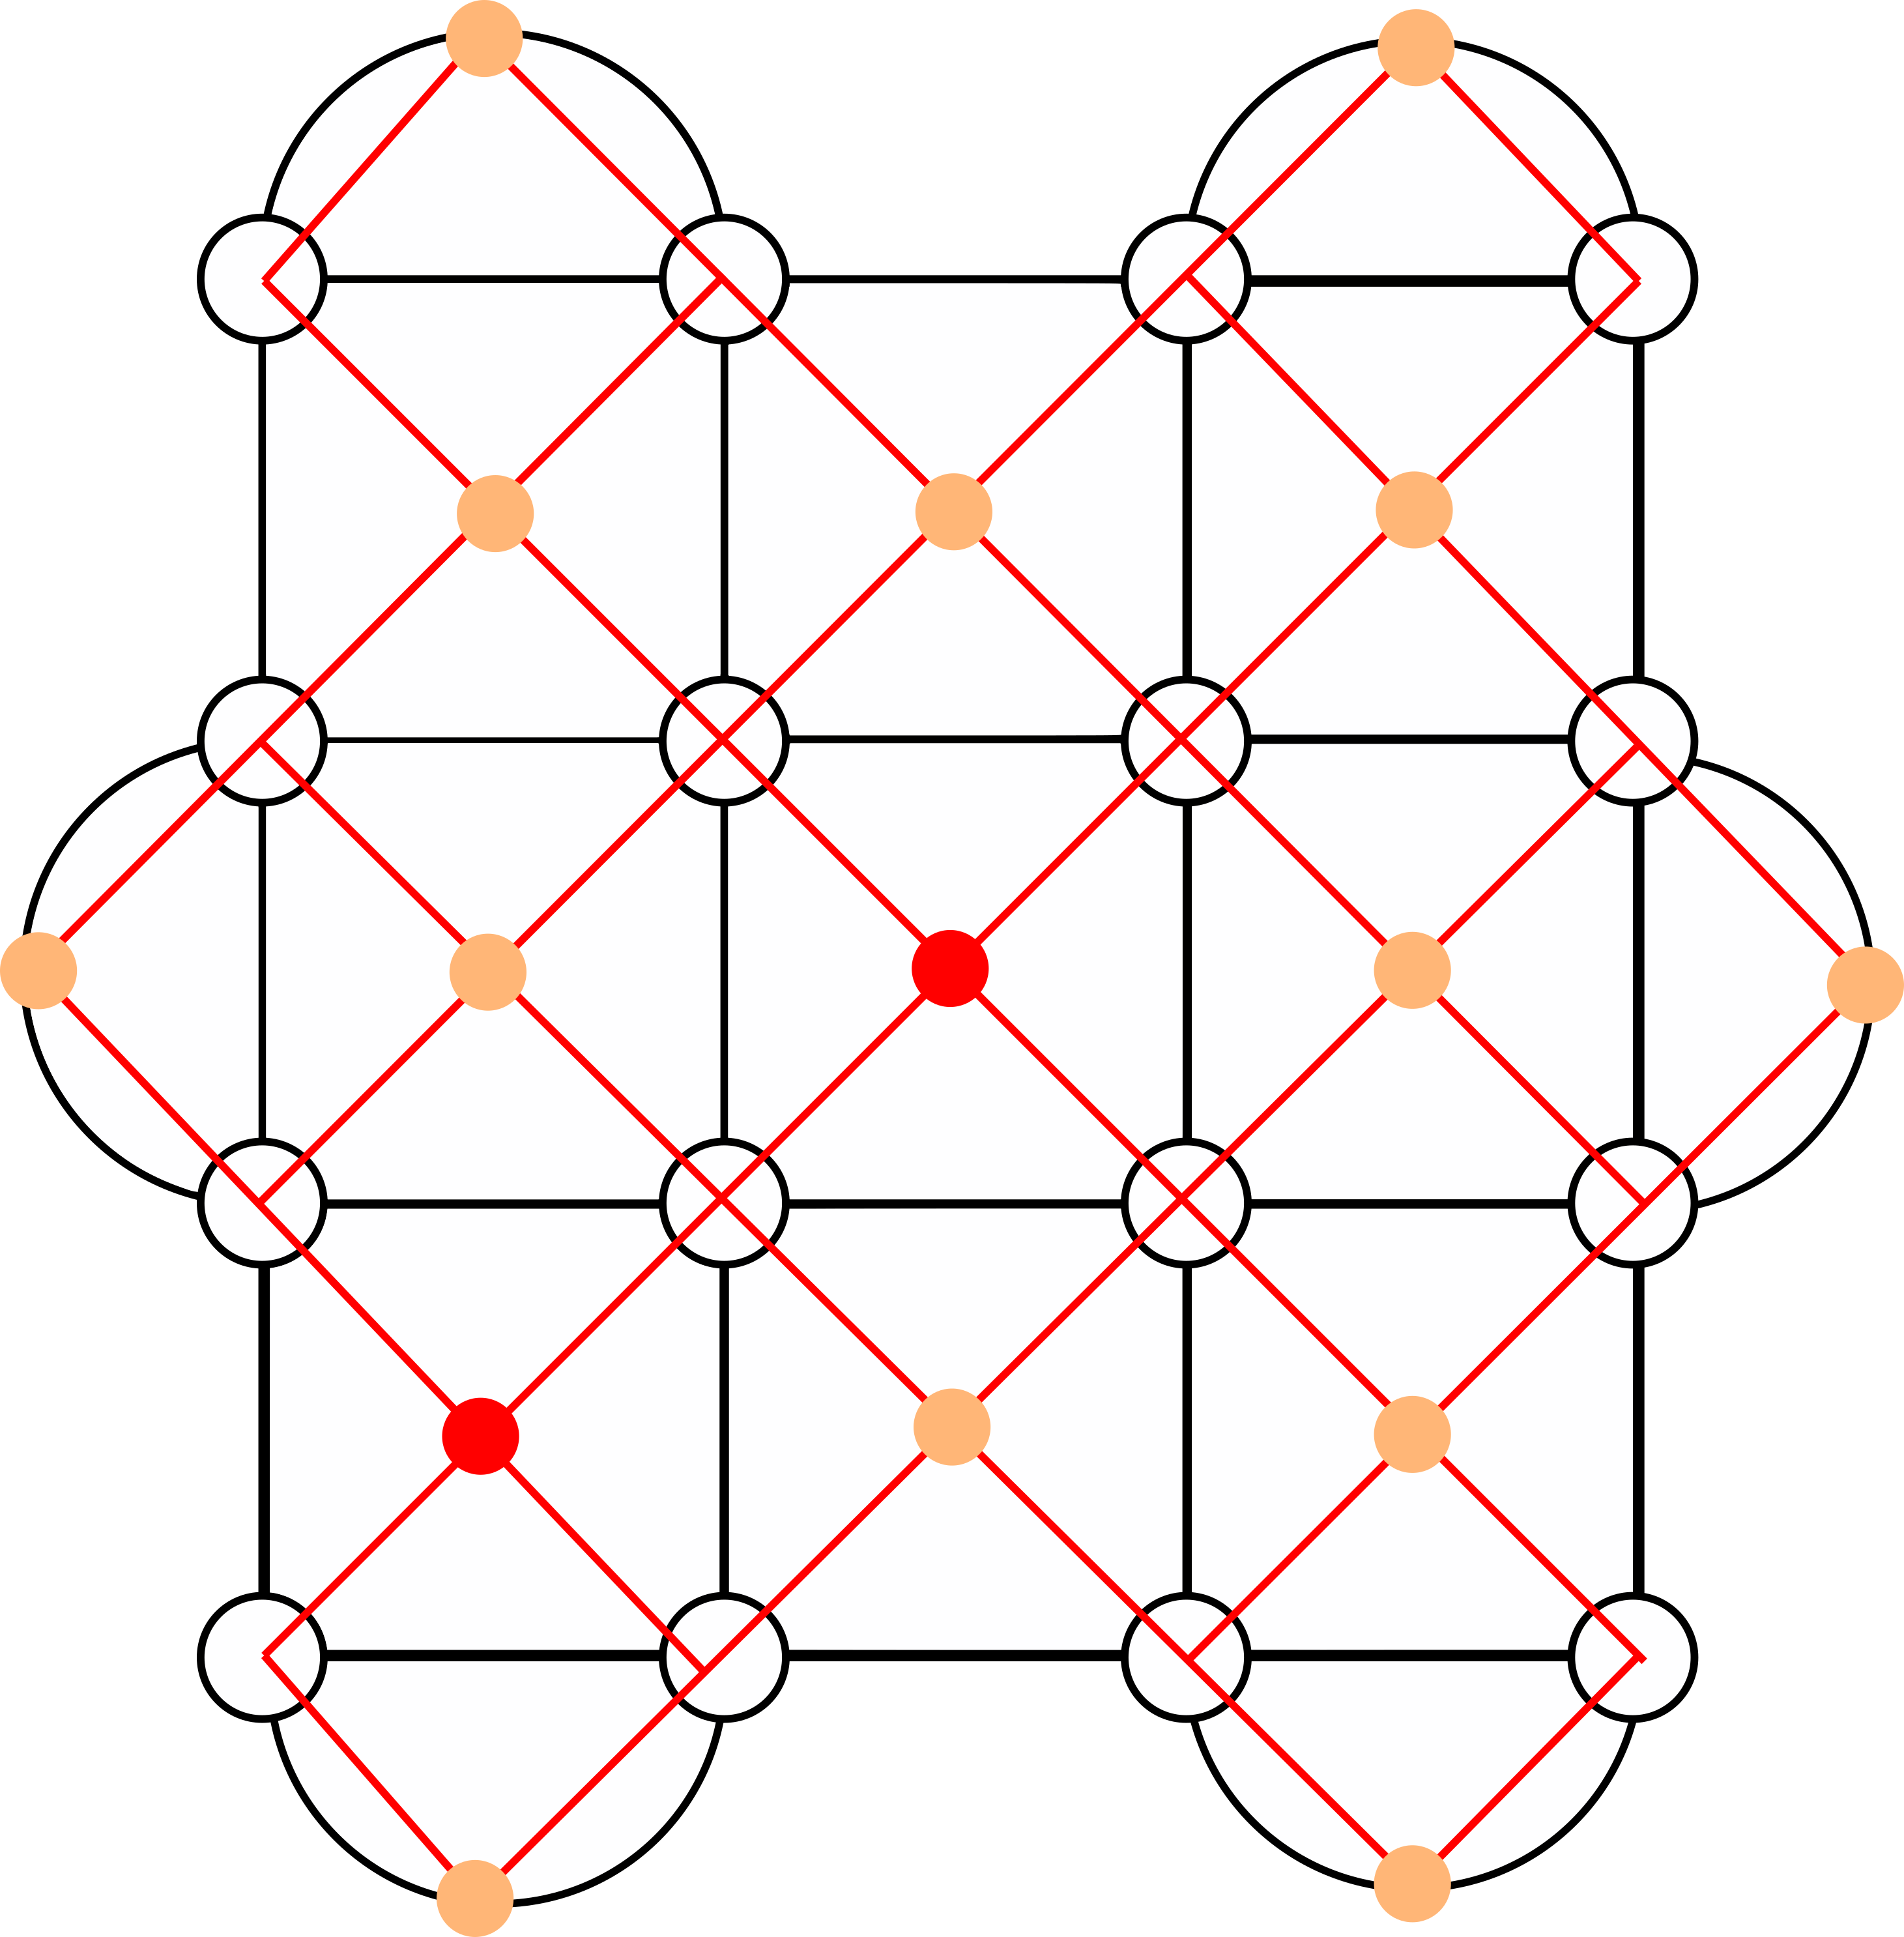
\includegraphics[width=0.55\textwidth]{fig/Rotated_surface_code_d4_decoder_graph_syndromes.png}
		\end{textblock*}
		\begin{textblock*}{9cm}(6cm,3.5cm)
			\textbf{Maximum Probability/Minimum Weight Perfect Matching Decoder~\citeauthoryear{edmonds_paths_1965}:}\\
			Select lowest weight error on decoder graph consistent with the partial error information
		\end{textblock*}
	}
	\only<5-5>{
		\begin{textblock*}{7cm}(1.5cm,2cm)
			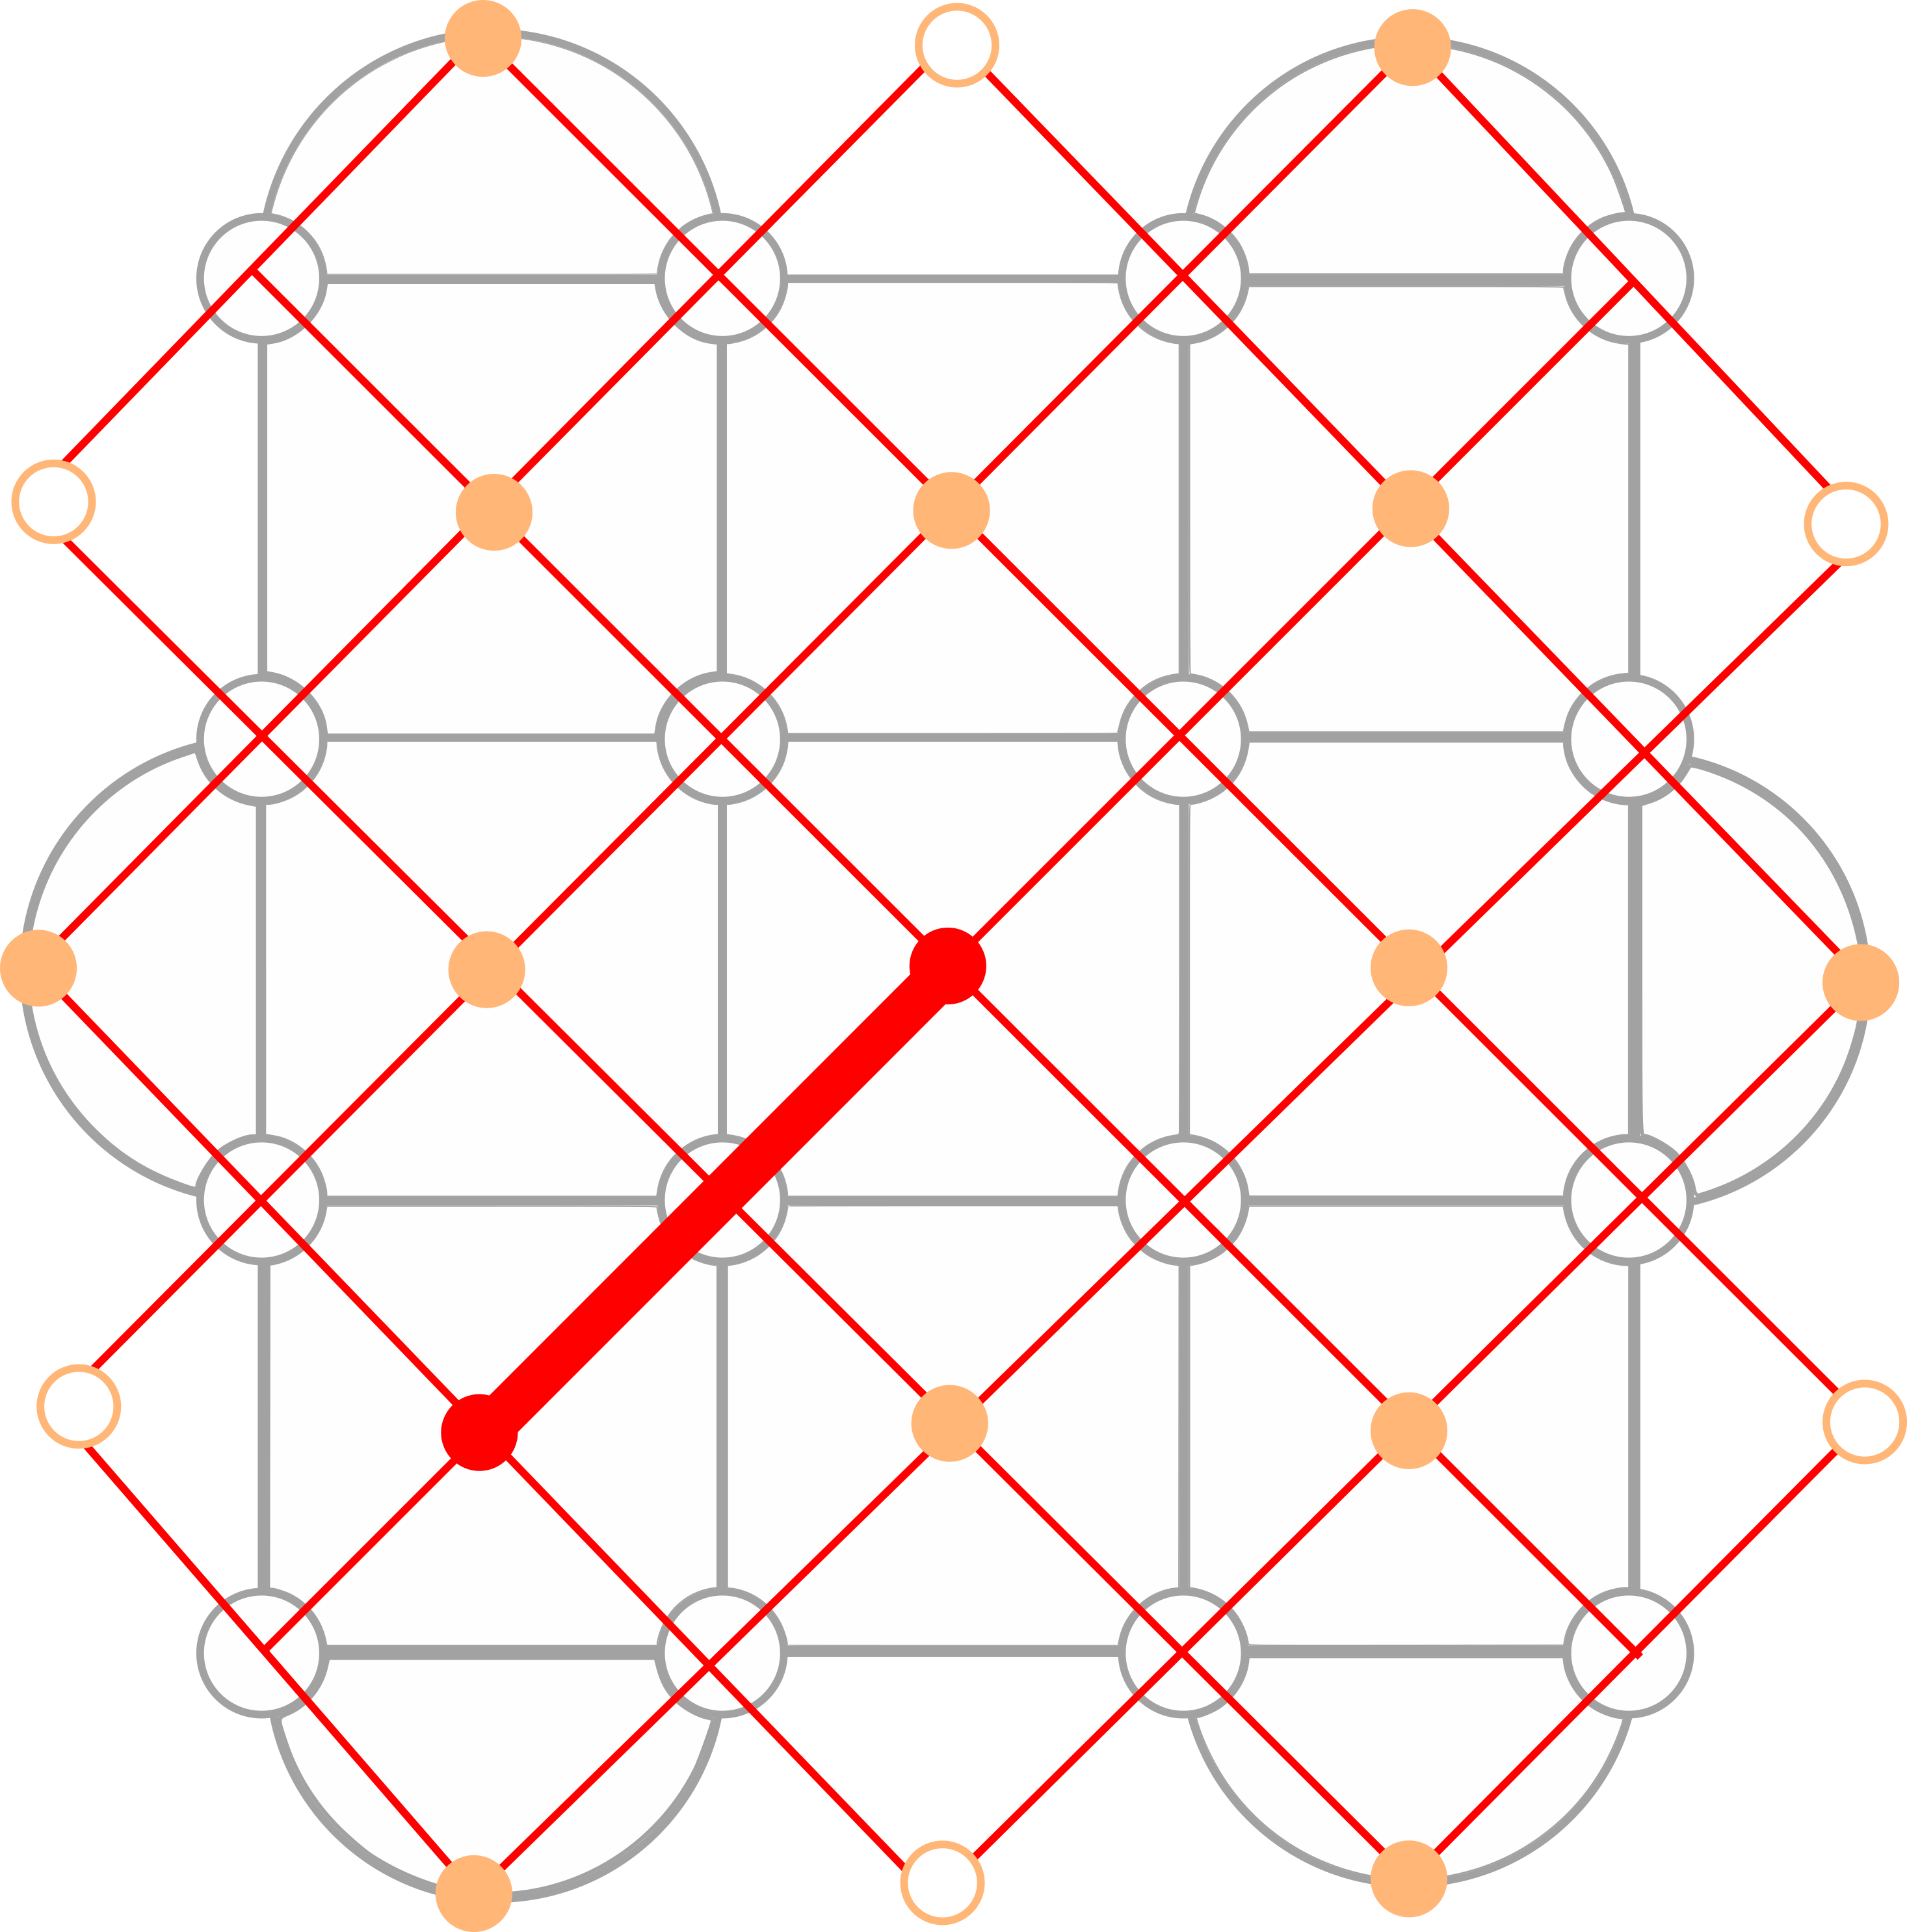
\includegraphics[width=0.55\textwidth]{fig/Rotated_surface_code_d4_decoder_graph_decoded.png}
		\end{textblock*}
		\begin{textblock*}{9cm}(6cm,3.5cm)
			\textbf{Maximum Probability/Minimum Weight Perfect Matching Decoder~\citeauthoryear{edmonds_paths_1965}:}\\
			Select lowest weight error on decoder graph consistent with the partial error information\\
		\end{textblock*}
		\begin{textblock*}{14cm}(1.5cm,6.5cm)
			The decoder estimates are not always correct! \\
			$\rightarrow$ Logical error rate $\equiv$ probability of correction failure $=$ $\langle\frac{\text{Number faulty error estimates}}{\text{Number estimates}}\rangle$\\
		\end{textblock*}
	}
\end{frame}

\begin{frame}{Scaling the system size}
	\vspace{10pt}
	\begin{center}
		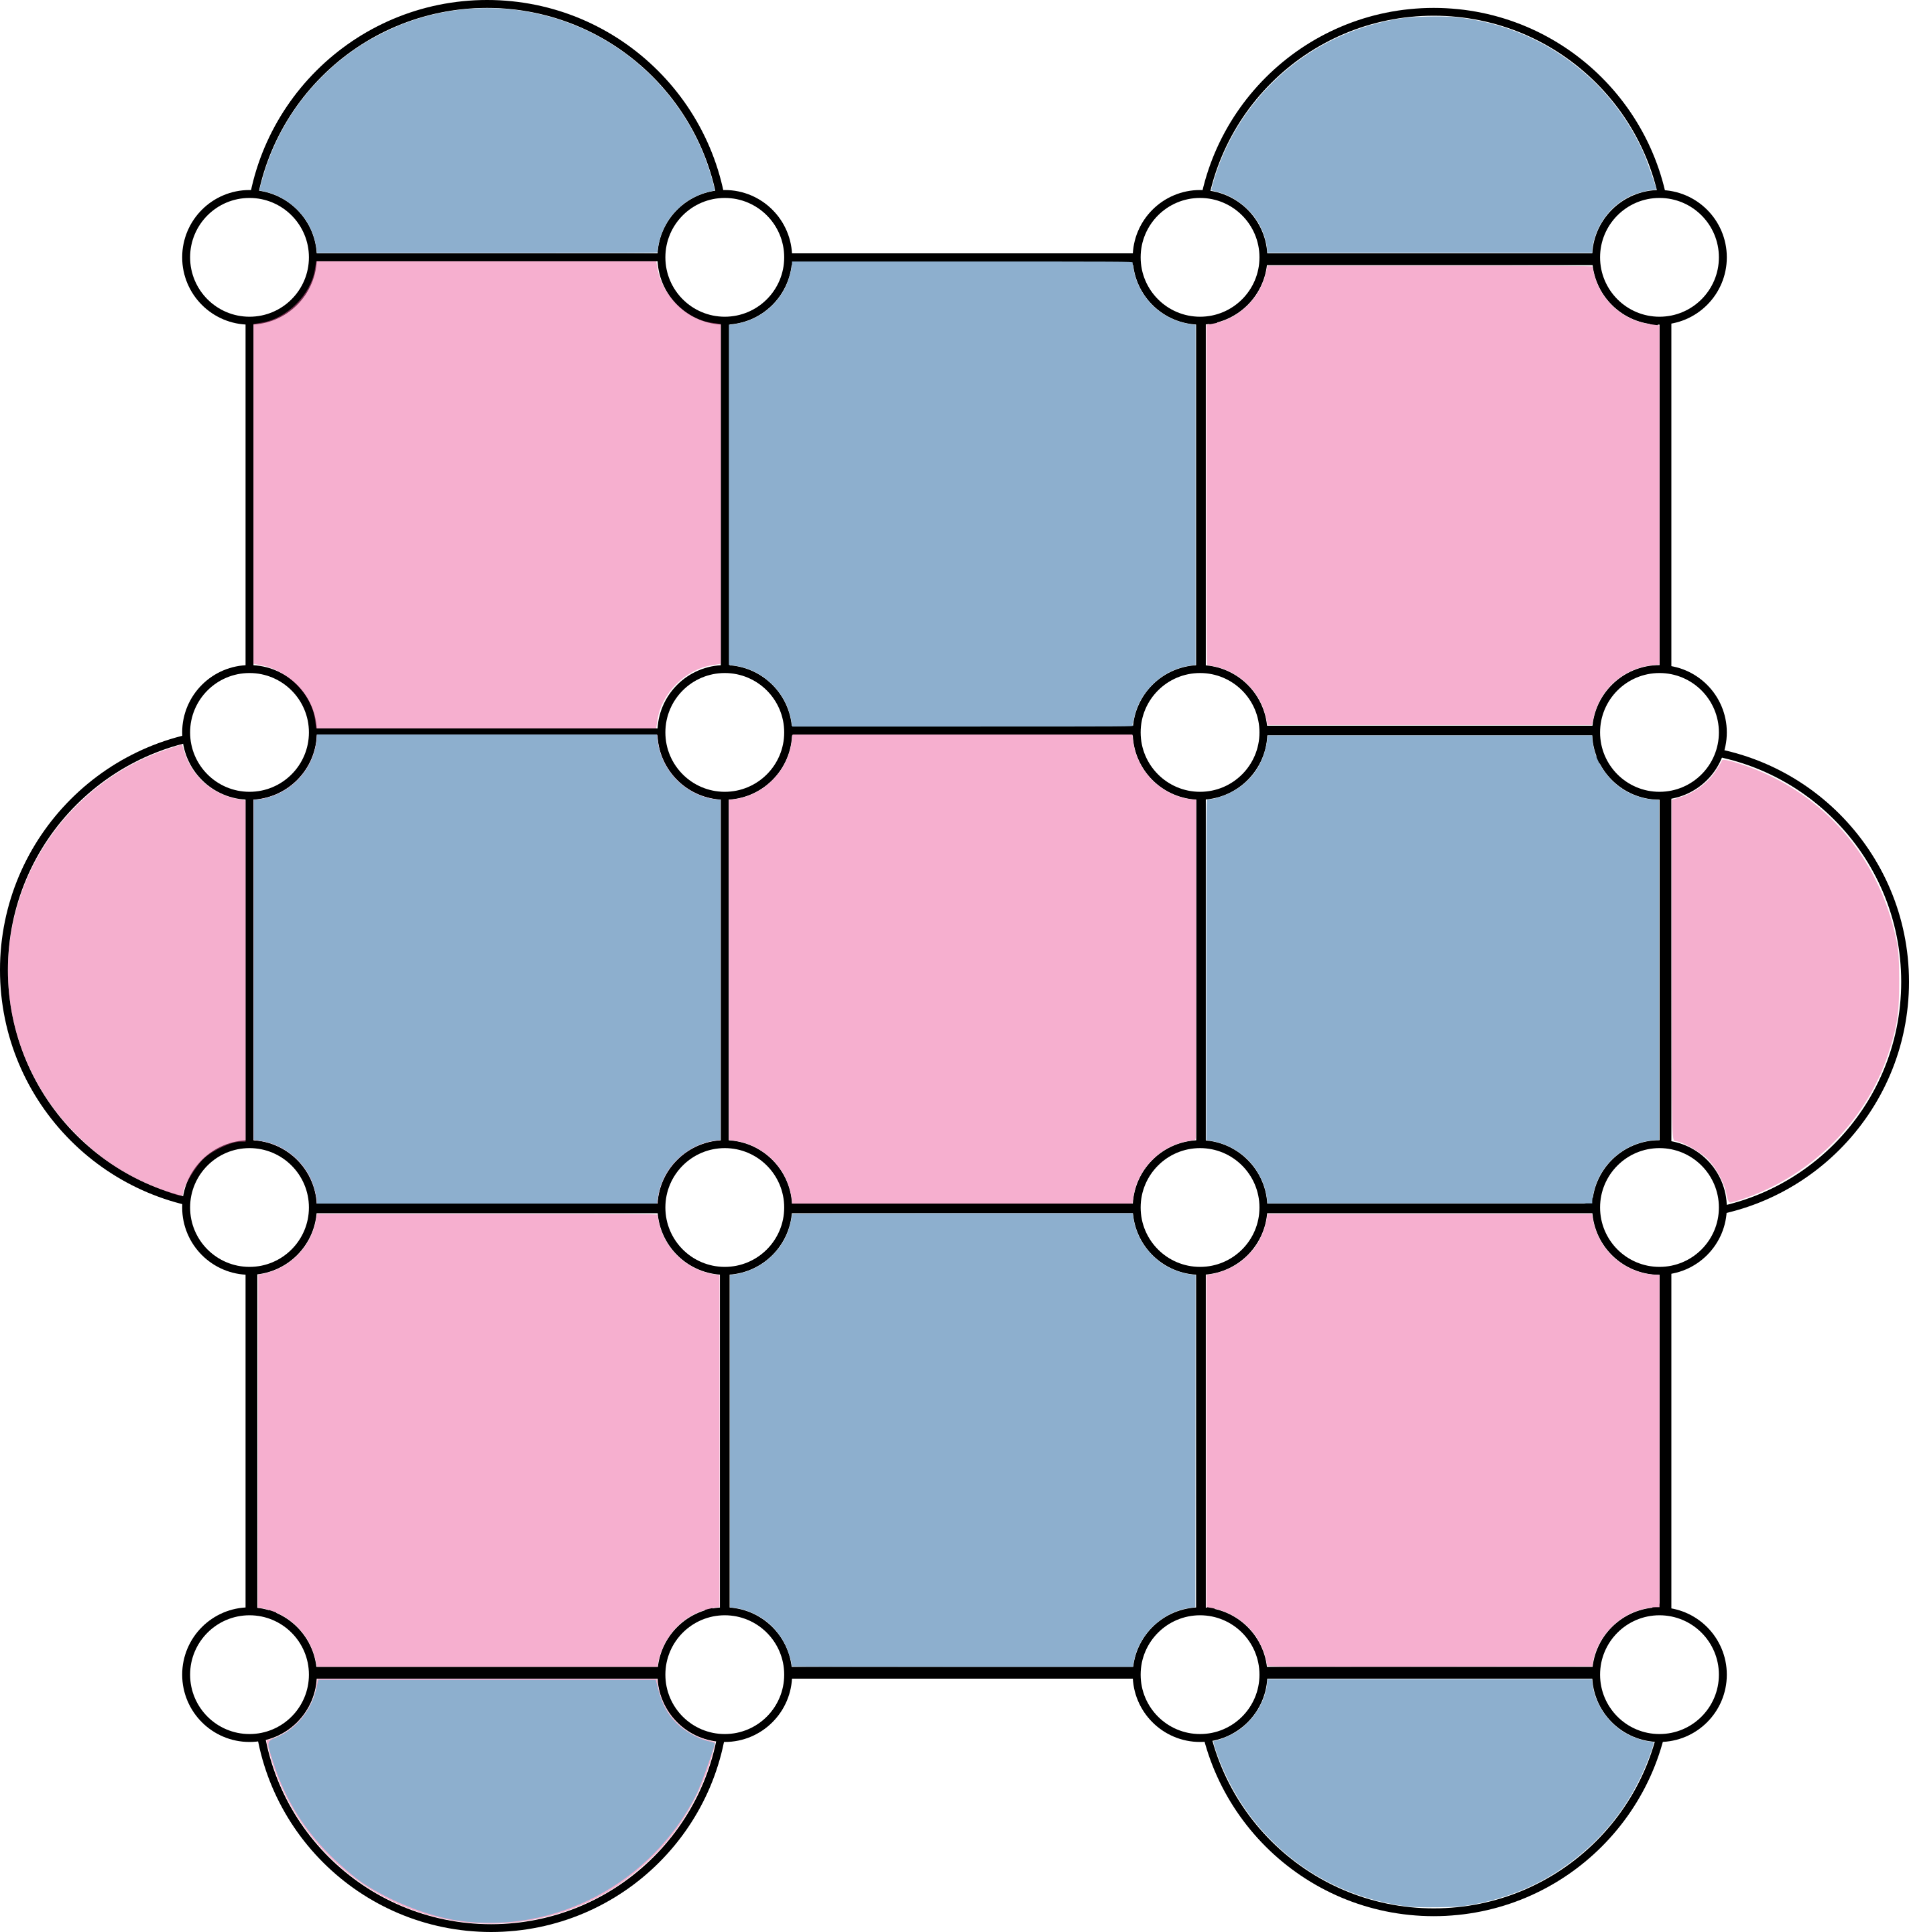
\includegraphics[width=0.12\textwidth]{fig/Rotated_surface_code_d4.png}
		\begin{tikzpicture}[overlay]
			\draw[->, line width=0.8mm, osakared] (1, 1) -- (8,1)
			node[midway, above, yshift=15pt, text=black] {Probability of error appearance increases}
            node[midway, below, yshift=-15pt, text=black] {Redundancy increases robustness of logical qubit};
		\end{tikzpicture}
		\hspace{9cm}
        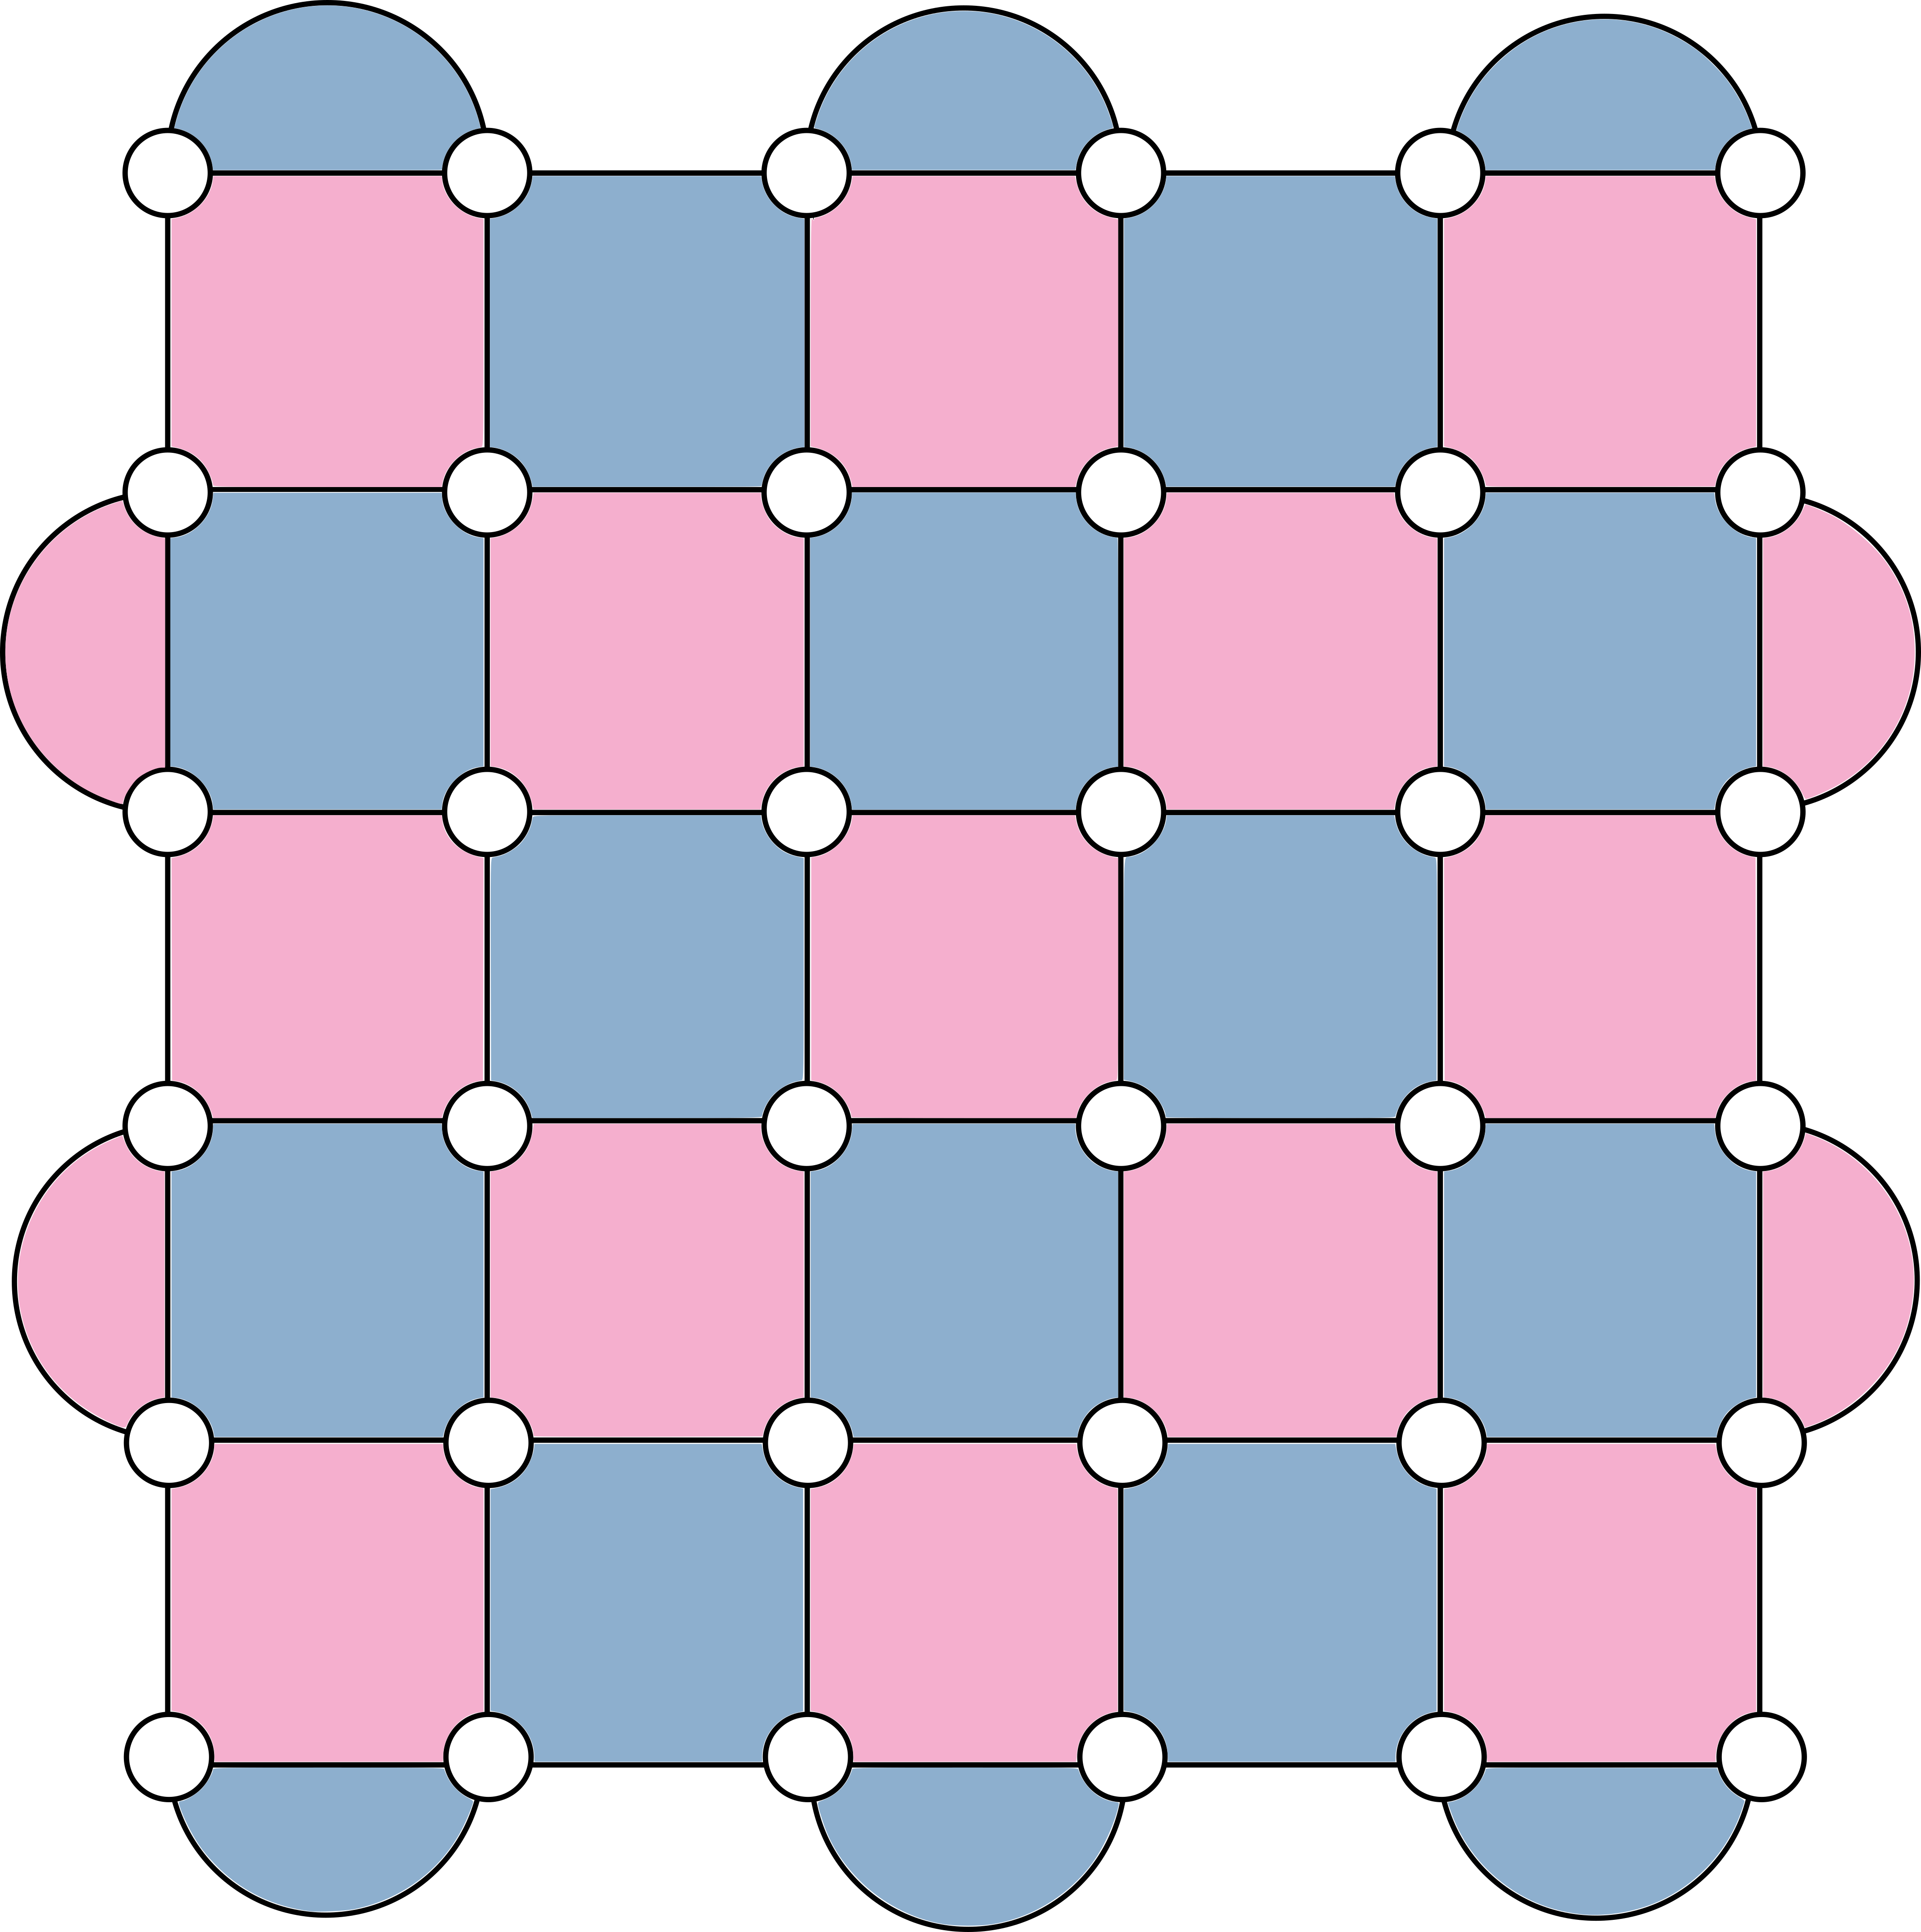
\includegraphics[width=0.12\textwidth]{fig/Rotated_surface_code_d6.png}
	\end{center}
	\pause
	\begin{center}
		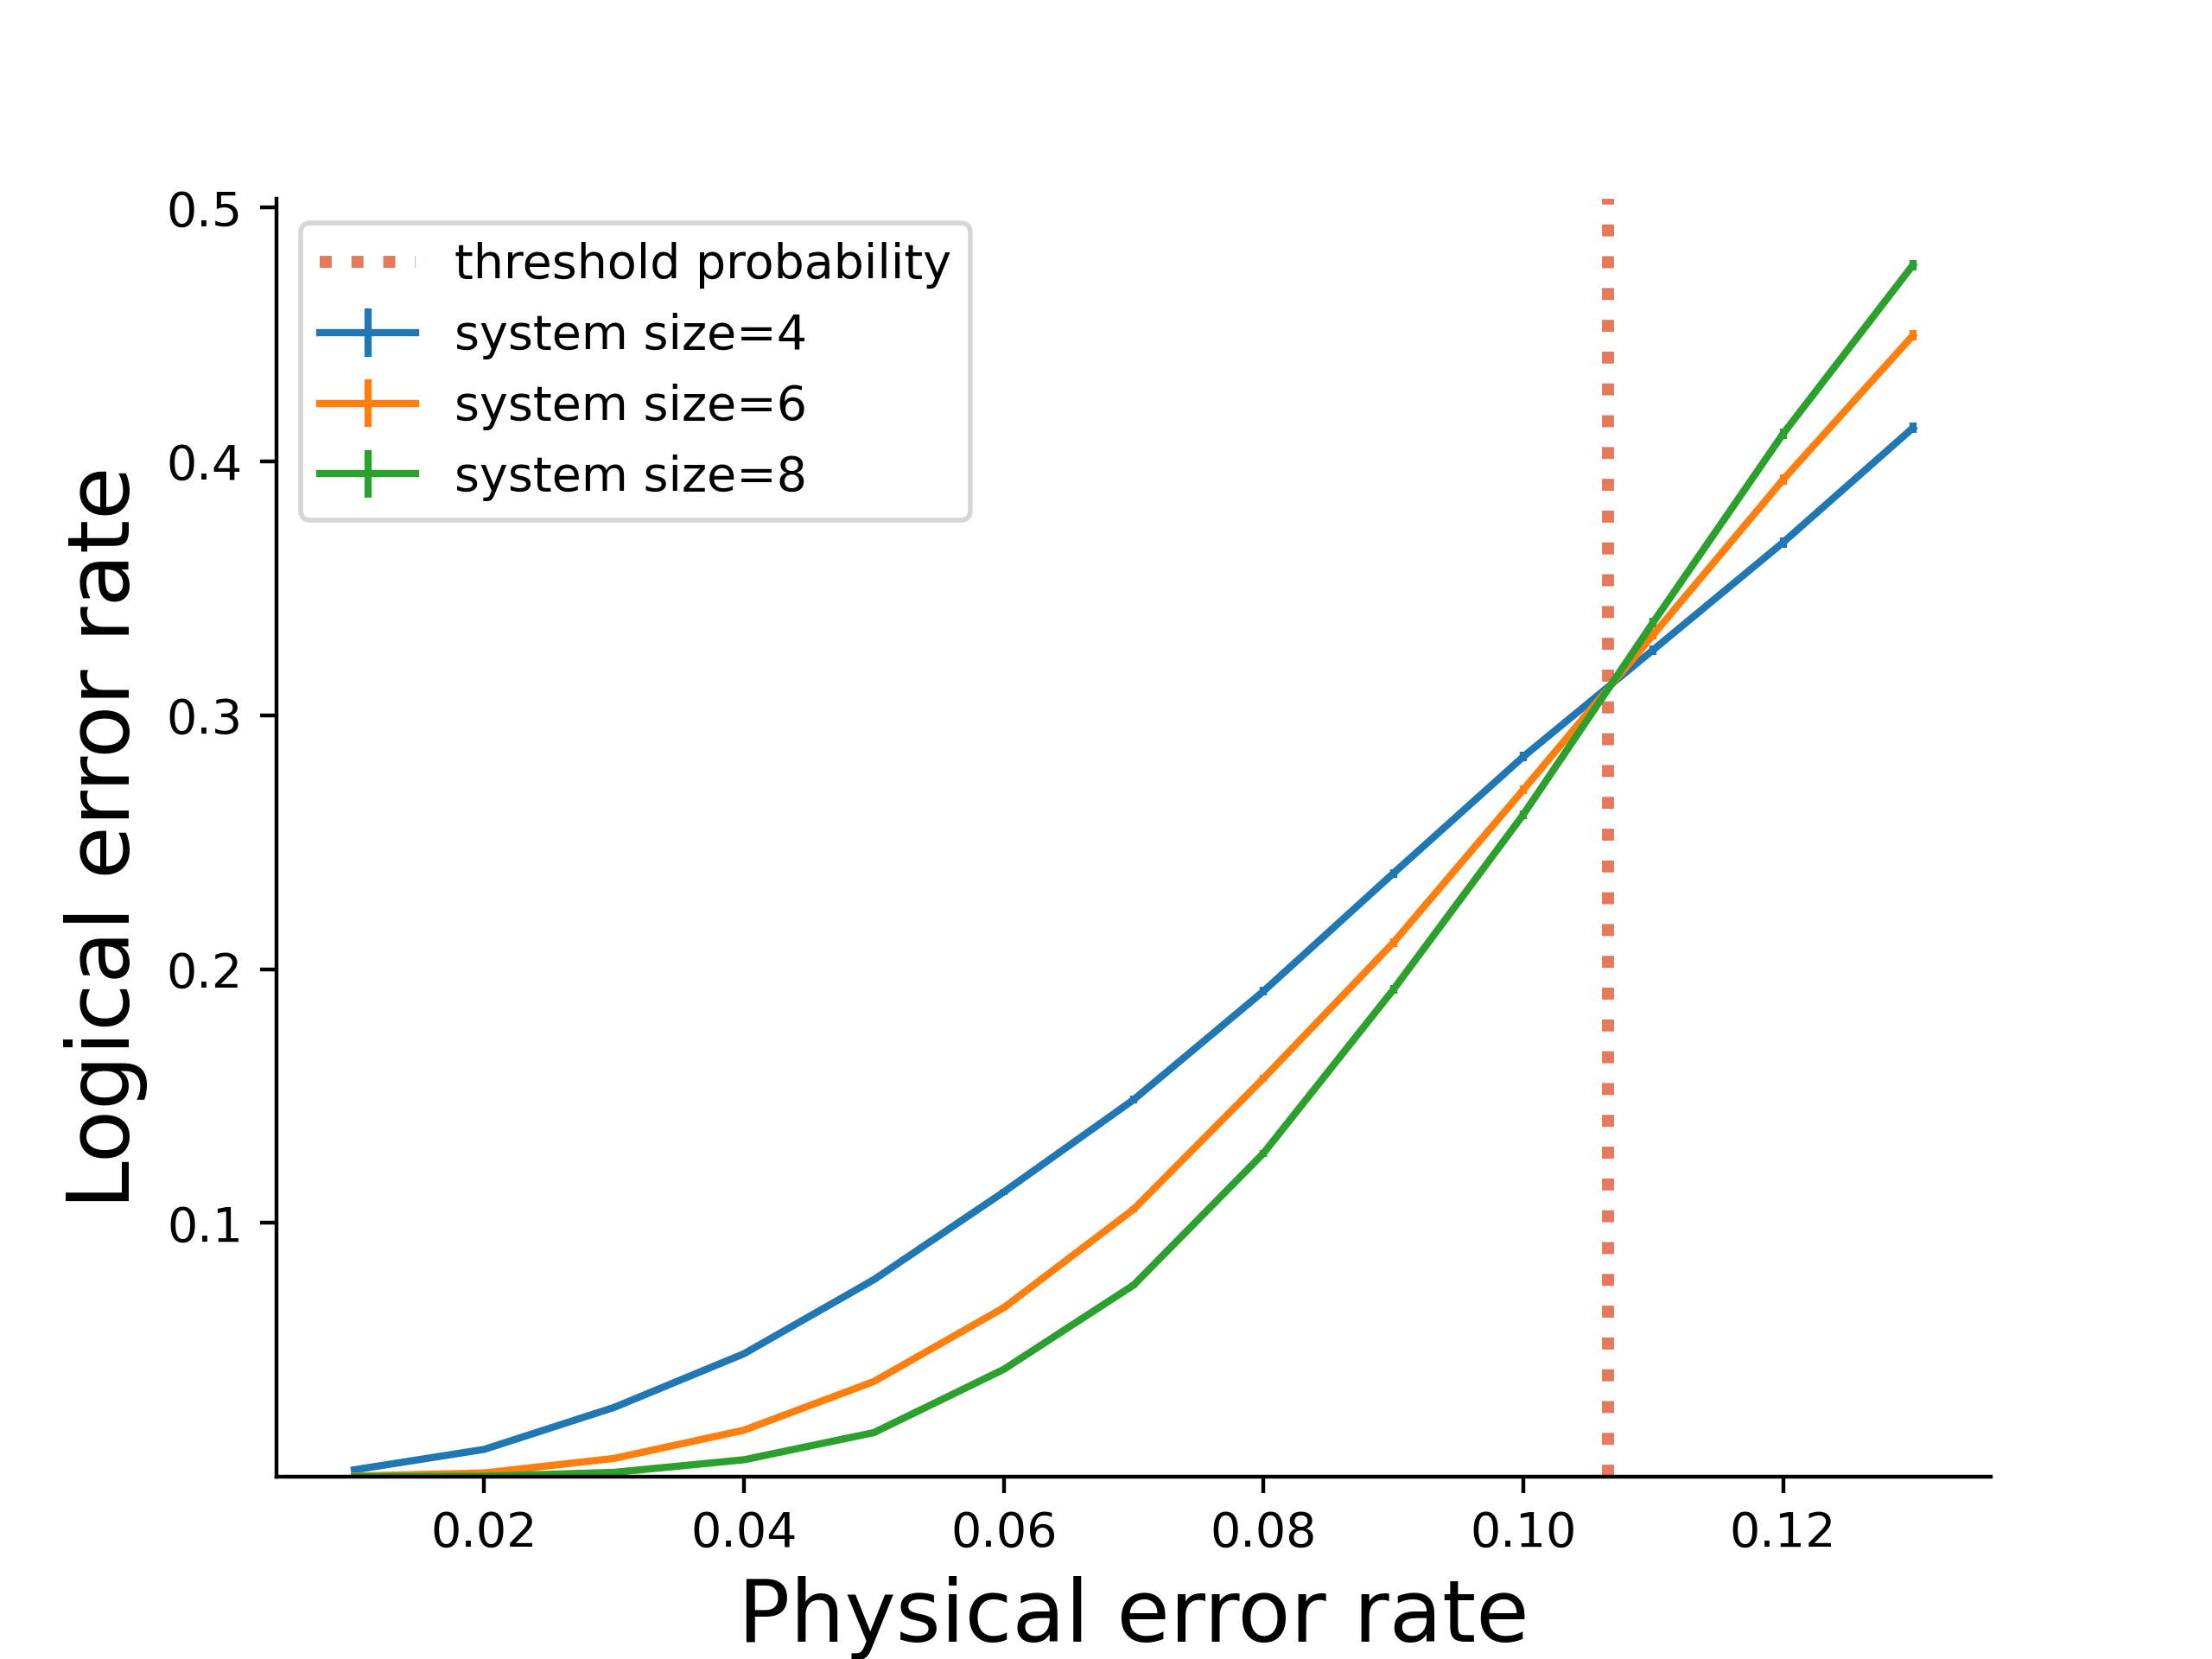
\includegraphics[width=0.4\textwidth]{fig/threshold.png}
		\hspace{0.5cm}
		\pause
        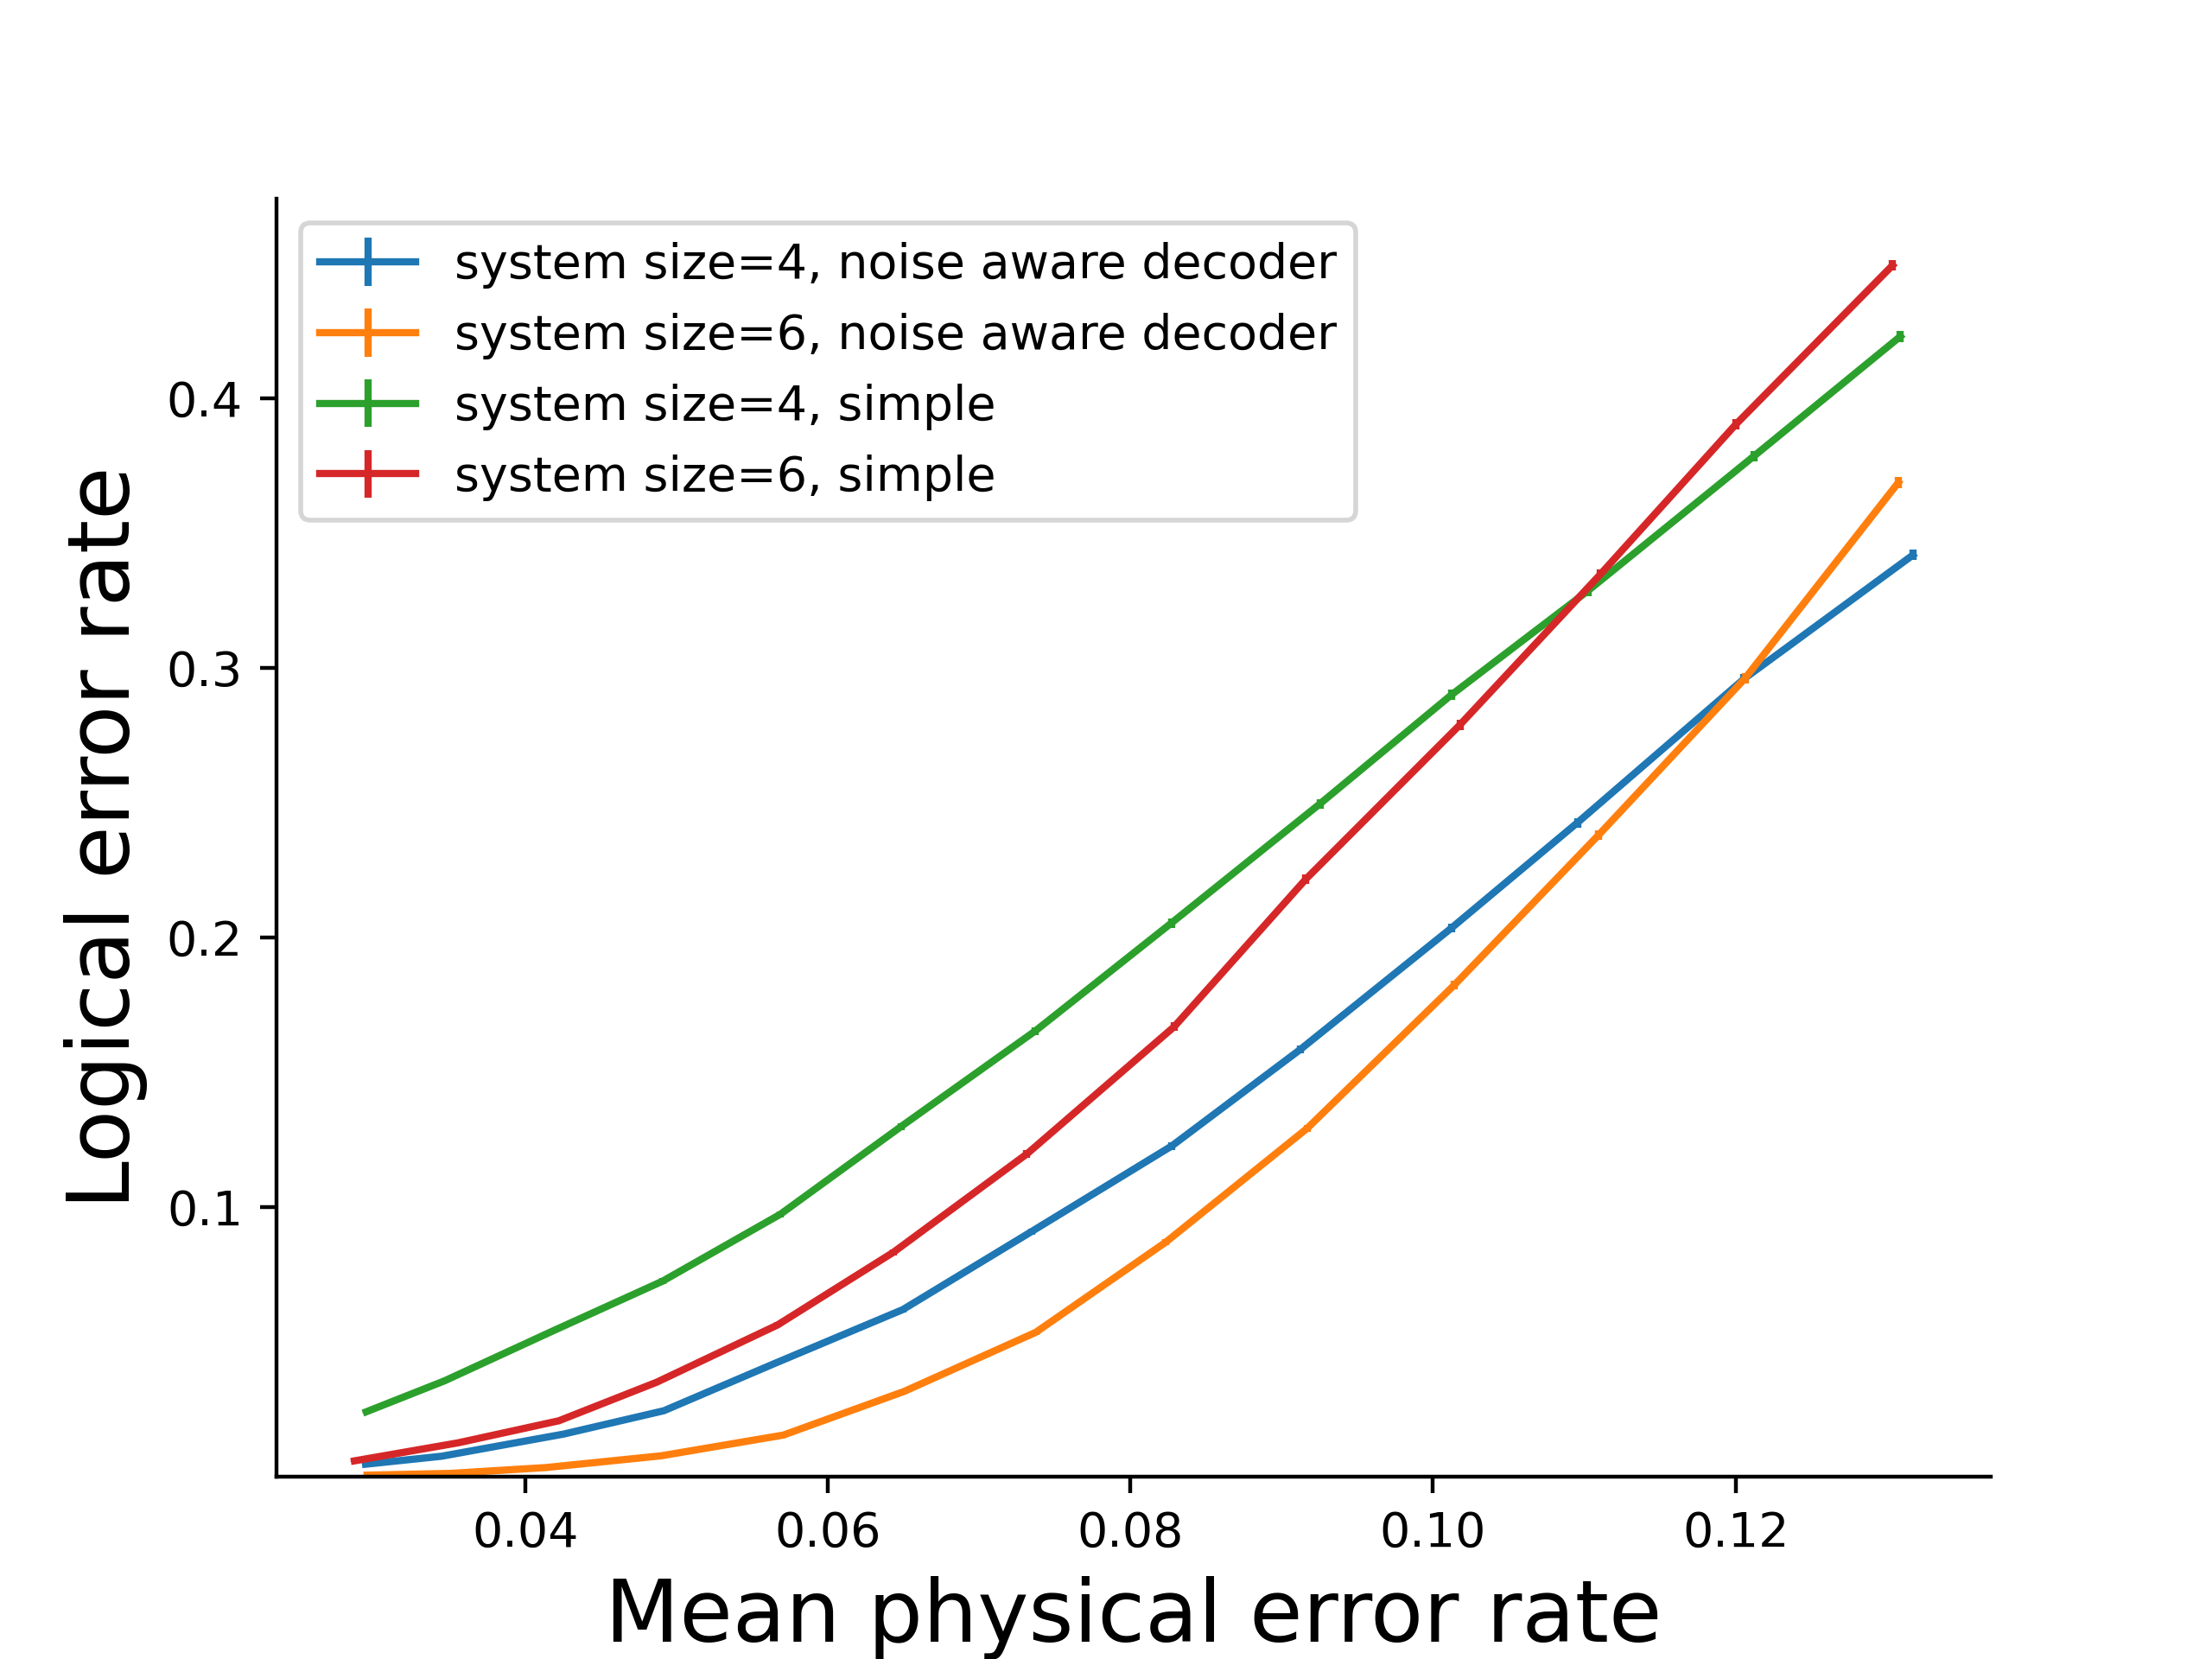
\includegraphics[width=0.4\textwidth]{fig/noise_aware.png}
	\end{center}
	\only<2-2>{
		\begin{textblock*}{6cm}(8cm,5.5cm)
			Existence proofs of thresholds have been established for specific code families~\citeauthoryear{knill_resilient_1997, kitaev_fault-tolerant_2003}.
		\end{textblock*}
	}
\end{frame}

\begin{frame}{Problem statement}
	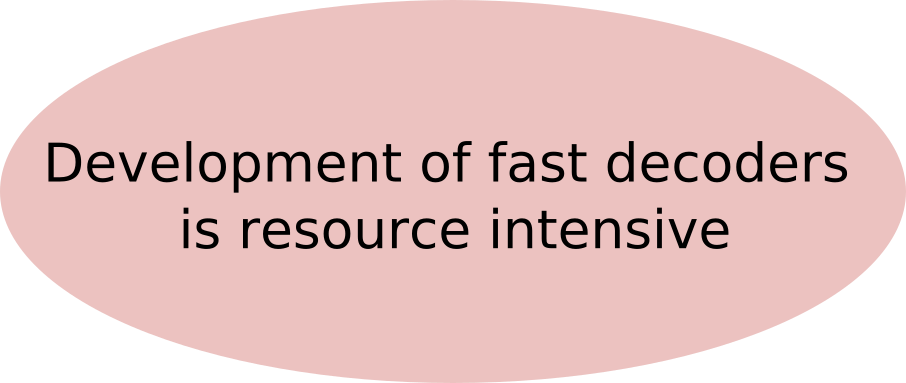
\includegraphics[width=0.4\textwidth]{fig/resource_intensive_decoder_dev.png}
	\only<1>{\hspace{20pt}\raisebox{35pt}{$\huge \Rightarrow$ \textbf{Only do it for promising codes}}}
	\only<2->{
		\hspace{2pt}
		\raisebox{18pt}{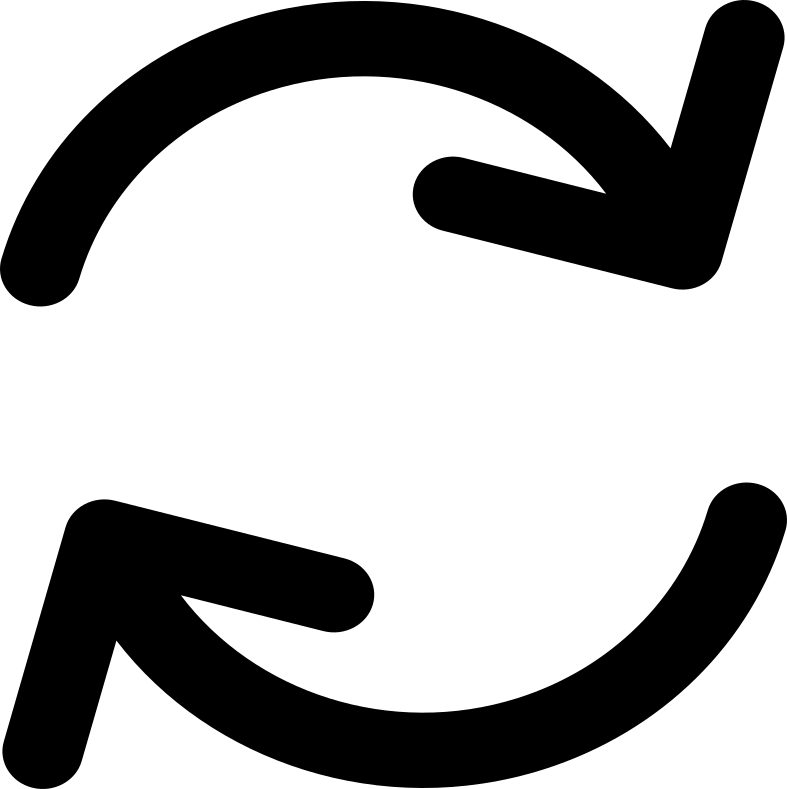
\includegraphics[width=0.08\textwidth]{fig/arrows.png}}
		\hspace{5pt}
		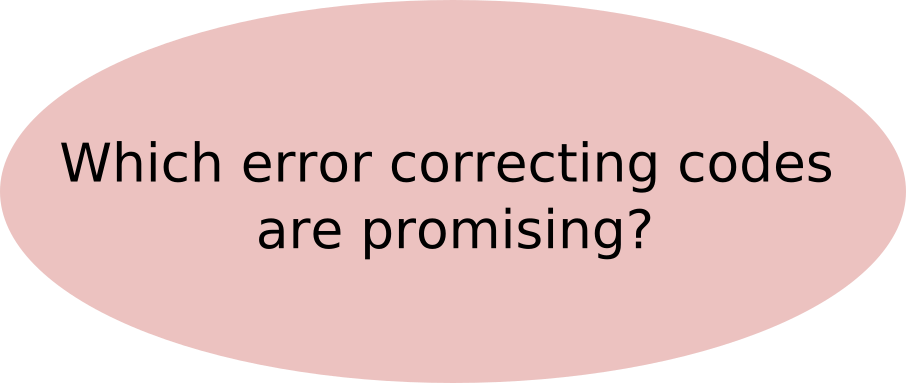
\includegraphics[width=0.4\textwidth]{fig/promising_codes.png}\\
	}
	\vspace{1.5cm}
	\only<3->{
	\center
	\textbf{Optimal code performance: \\baseline for code selection and decoder optimization}
	% \begin{itemize}
	% 	\only<3->{\item \textbf{Code selection:} Hardware specific simulation of optimal code performance makes error correcting codes comparable.}
	% 	\only<4>{\item \textbf{Decoder optimization:} Estimation of optimal code performance shows upper limit for decoder optimization.}
	% \end{itemize}
	}
\end{frame}

\begin{frame}{Approximate Optimal Decoding}
	\textbf{Tensor Network Decoder~\citeauthoryear{bravyi_efficient_2014}}
		\begin{itemize}
			\item Surface Code $\rightarrow$ Tensor Network
			\item Optimal decoding $\rightarrow$ TN contraction
			\item Approximate contraction $\rightarrow$ approximate optimal decoding
			\item Generalised to arbitrary 2D codes \citeauthoryear{chubb_general_2021}
			\item Noise aware~\citeauthoryear{darmawan_optimal_2024}
		\end{itemize}
\end{frame}



\begin{frame}{Suboptimal vs Optimal Decoding}
	\only<1-1>{
	\begin{textblock*}{10cm}(9.5cm,3cm)
		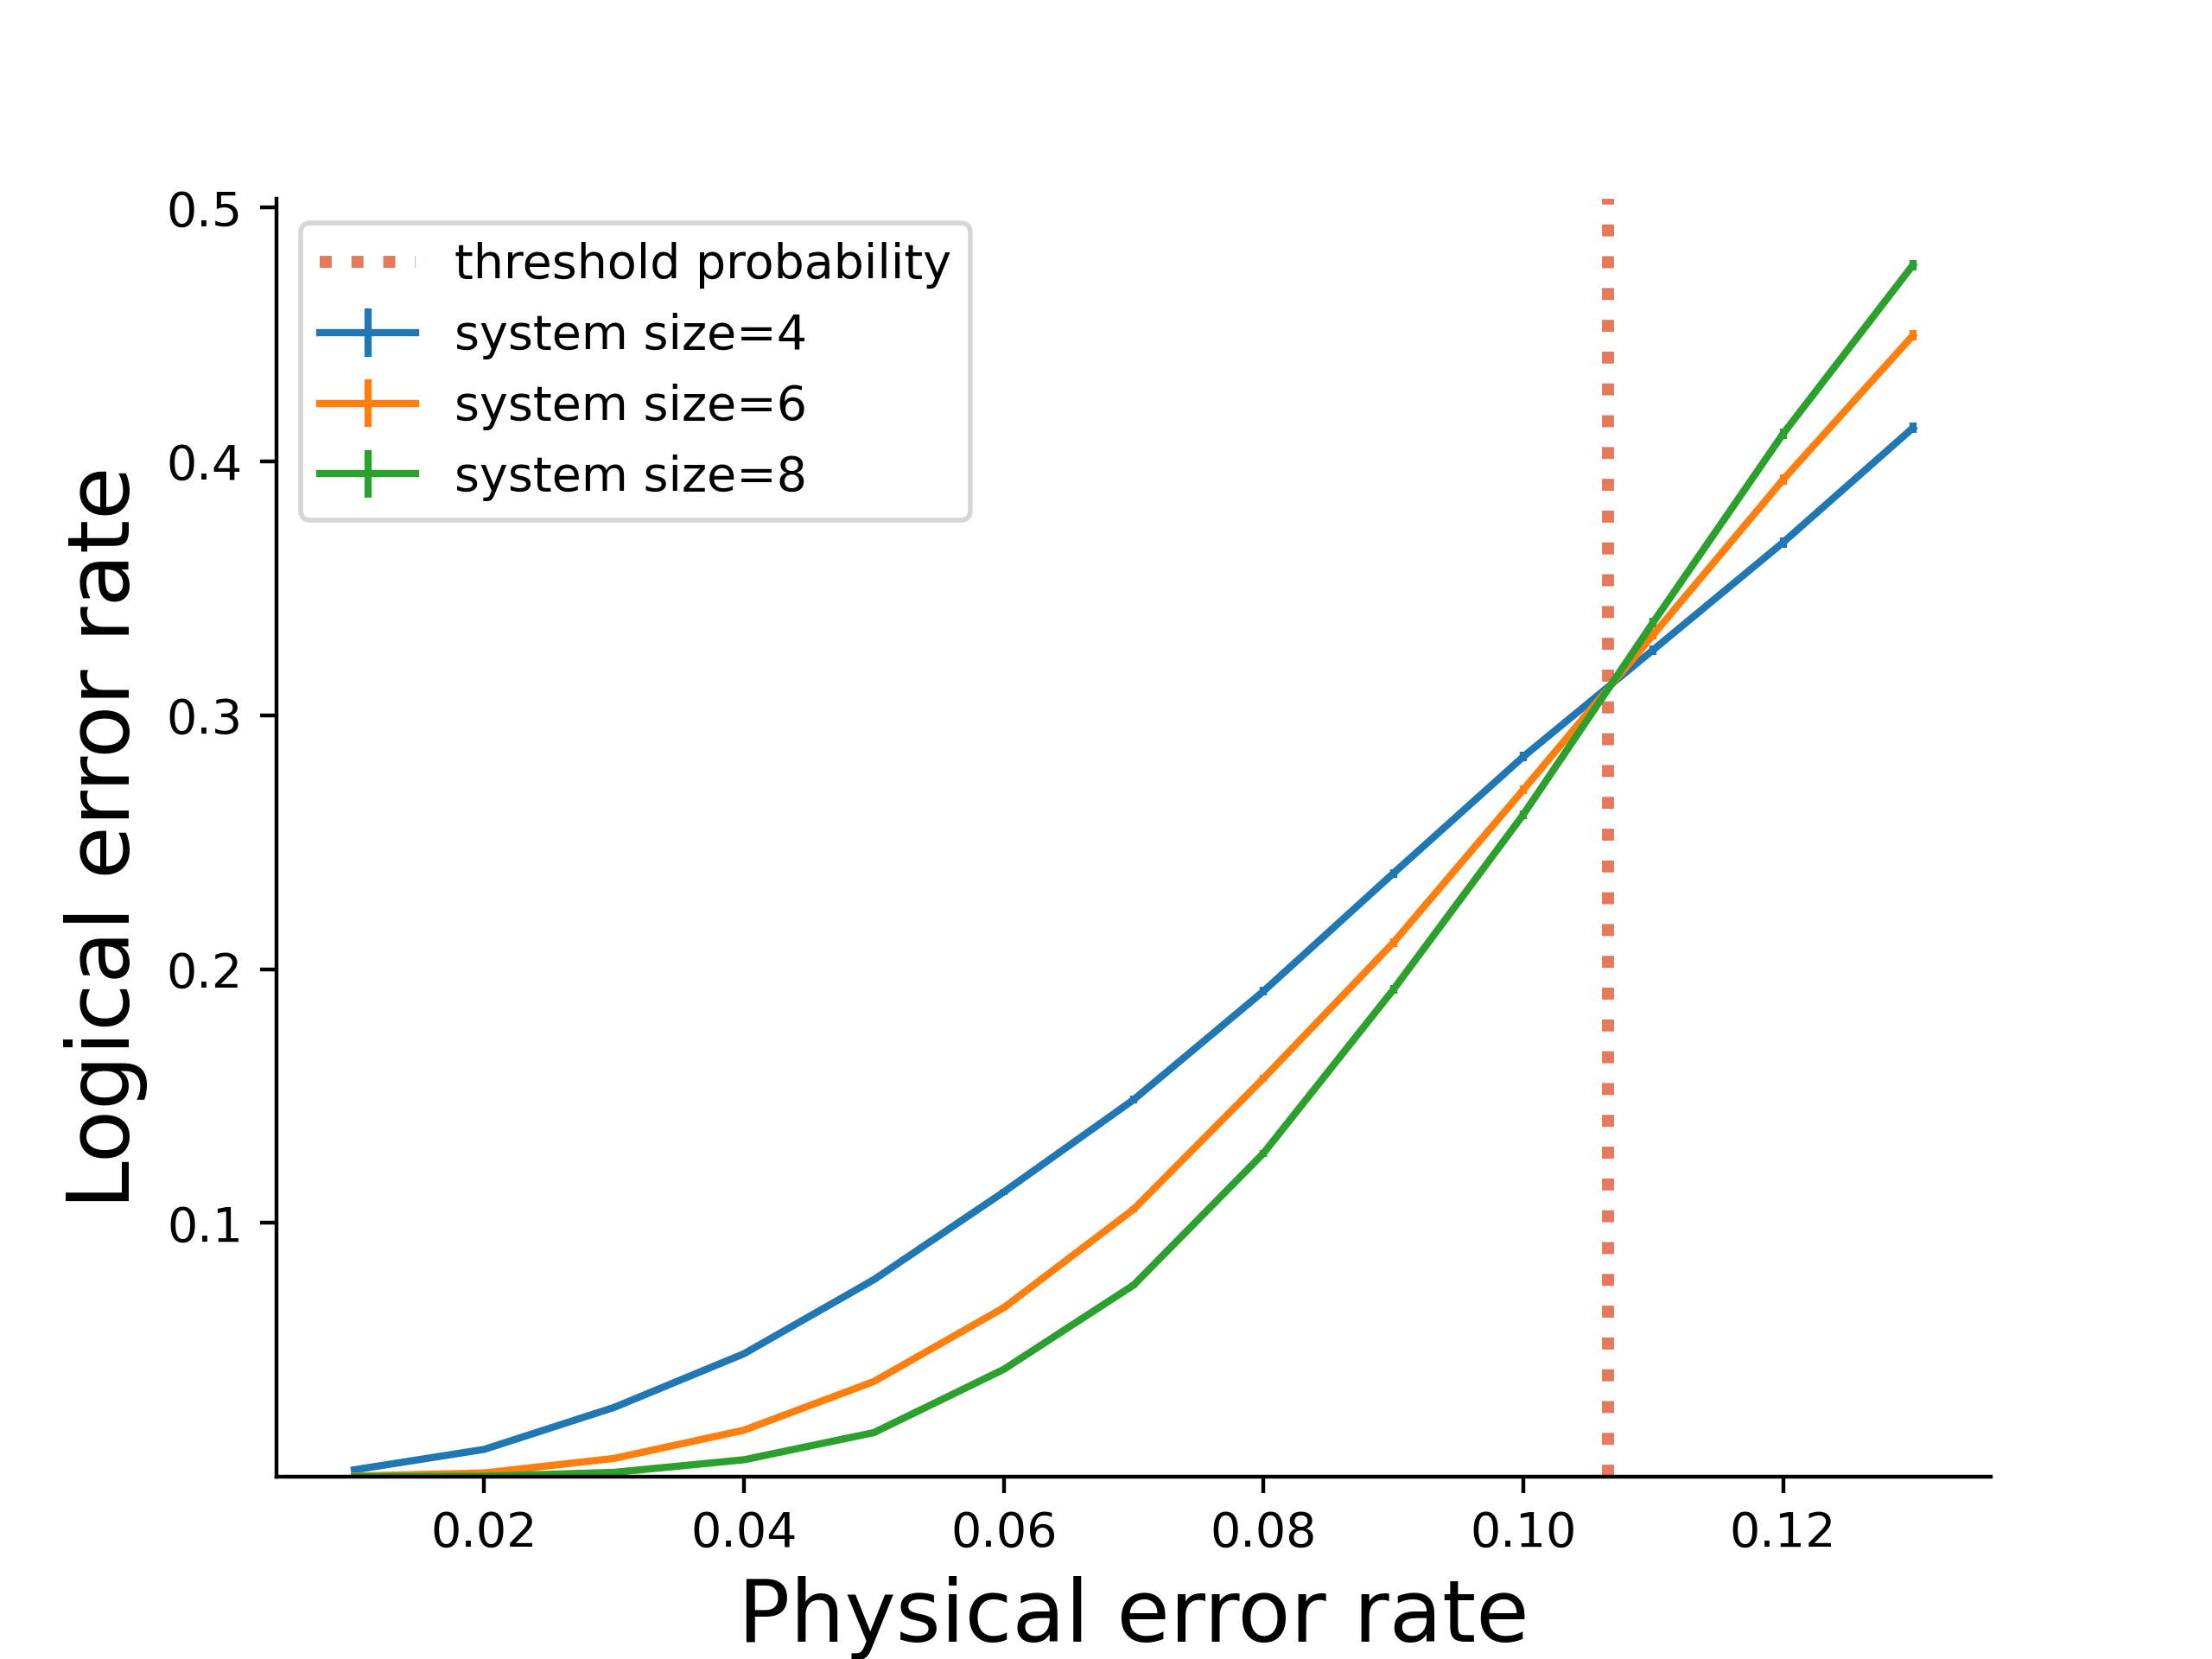
\includegraphics[width=0.5\textwidth]{fig/threshold.png}
	\end{textblock*}
	\begin{textblock*}{8cm}(0.5cm,4cm)
		\textbf{Suboptimal decoders:}\\
		Failure curves estimated for various finite sized codes under varying noise models~\citeauthoryear{demarti_iolius_decoding_2024}
	\end{textblock*}
	}
	\only<2-2>{
	\begin{textblock*}{10cm}(9.5cm,3cm)
		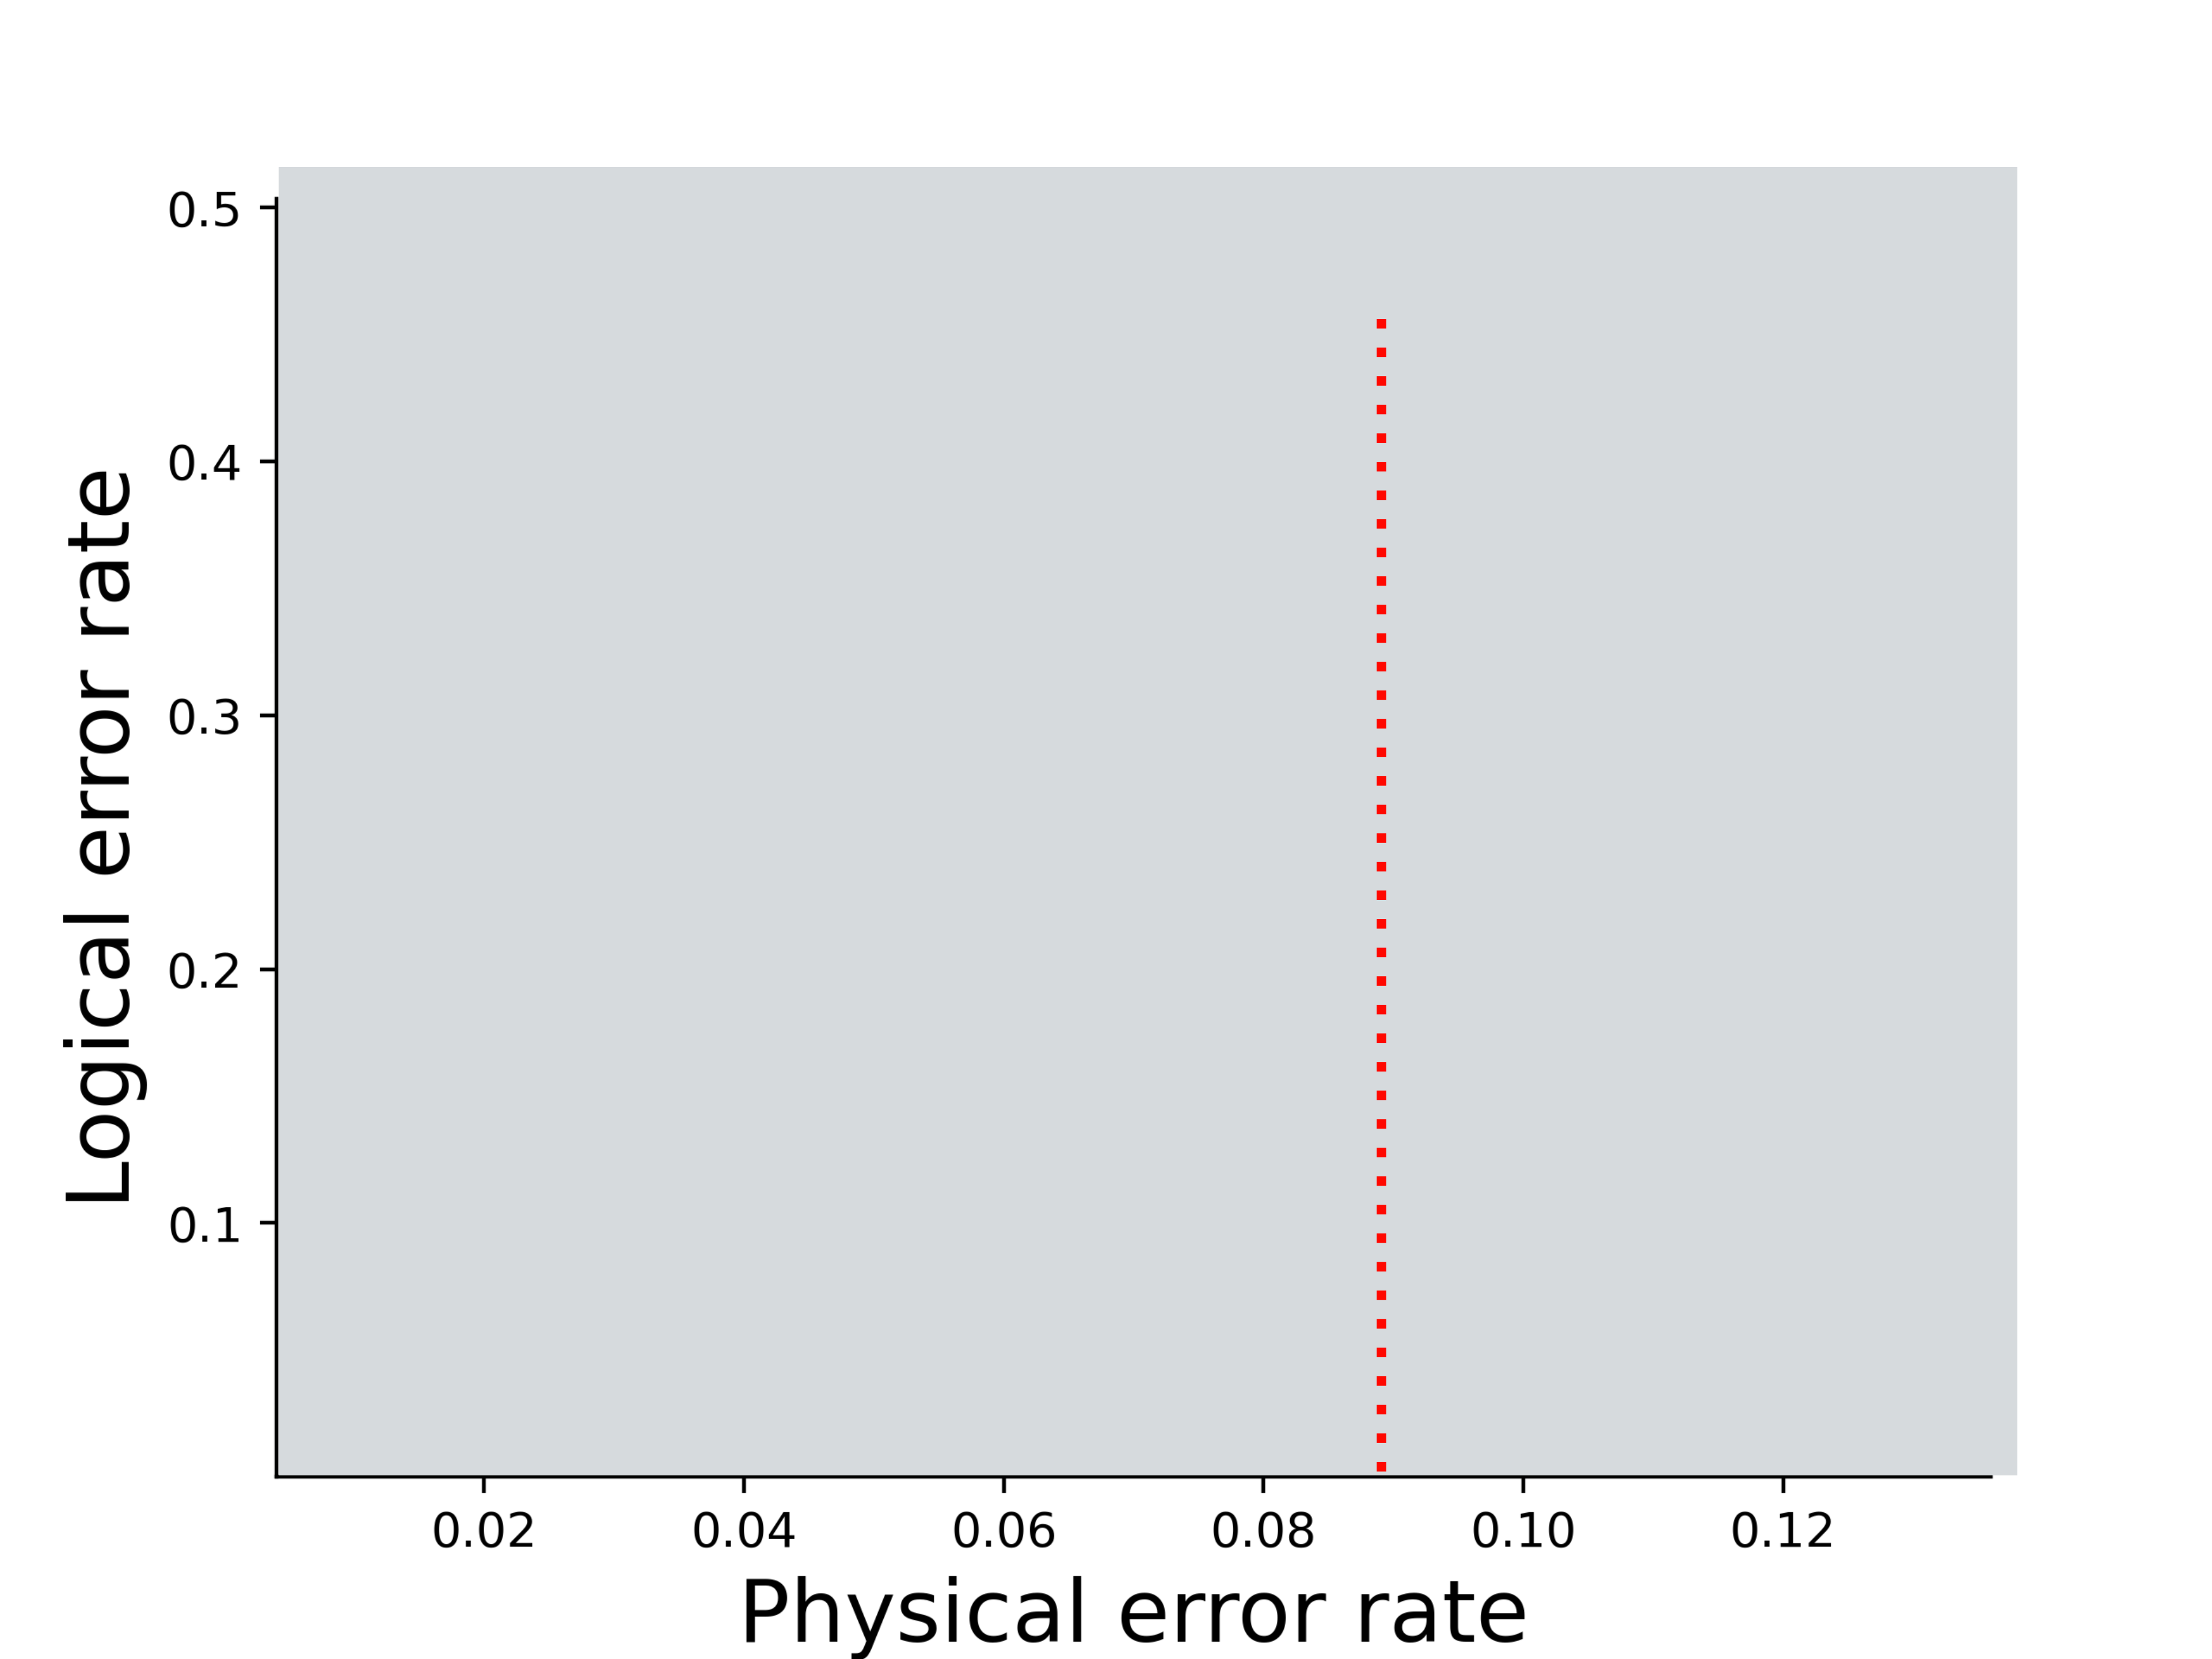
\includegraphics[width=0.5\textwidth]{fig/optimal_threshold.png}
	\end{textblock*}
	\begin{textblock*}{8cm}(0.5cm,3cm)
		\textbf{Optimal decoding:}\\
		Focus on optimal error threshold estimation
		\begin{itemize}
			\item Surface code under biflip noise~\citeauthoryear{merz_two-dimensional_2001} % mapping of the two-dimensional Ising model with random exchange (RBIM), via the transfer matrix, to a network model for a disordered system of non-interacting fermions. The RBIM transforms in this way to a localisation problem belonging to one of a set of non-standard symmetry classes, known as class D; the transition between paramagnet and ferromagnet is equivalent to a delocalisation transition between an insulator and a quantum Hall conductor.
			\item Color code under bitflip noise~\citeauthoryear{katzgraber_error_2009}
			\item Toric code under depolarization noise~\citeauthoryear{bombin_strong_2012}
			\item Surface code under mildly correlated bitflip noise~\citeauthoryear{chubb_statistical_2019}
		\end{itemize}
	\end{textblock*}
	}
	\only<3->{
	\begin{textblock*}{10cm}(9.5cm,3cm)
		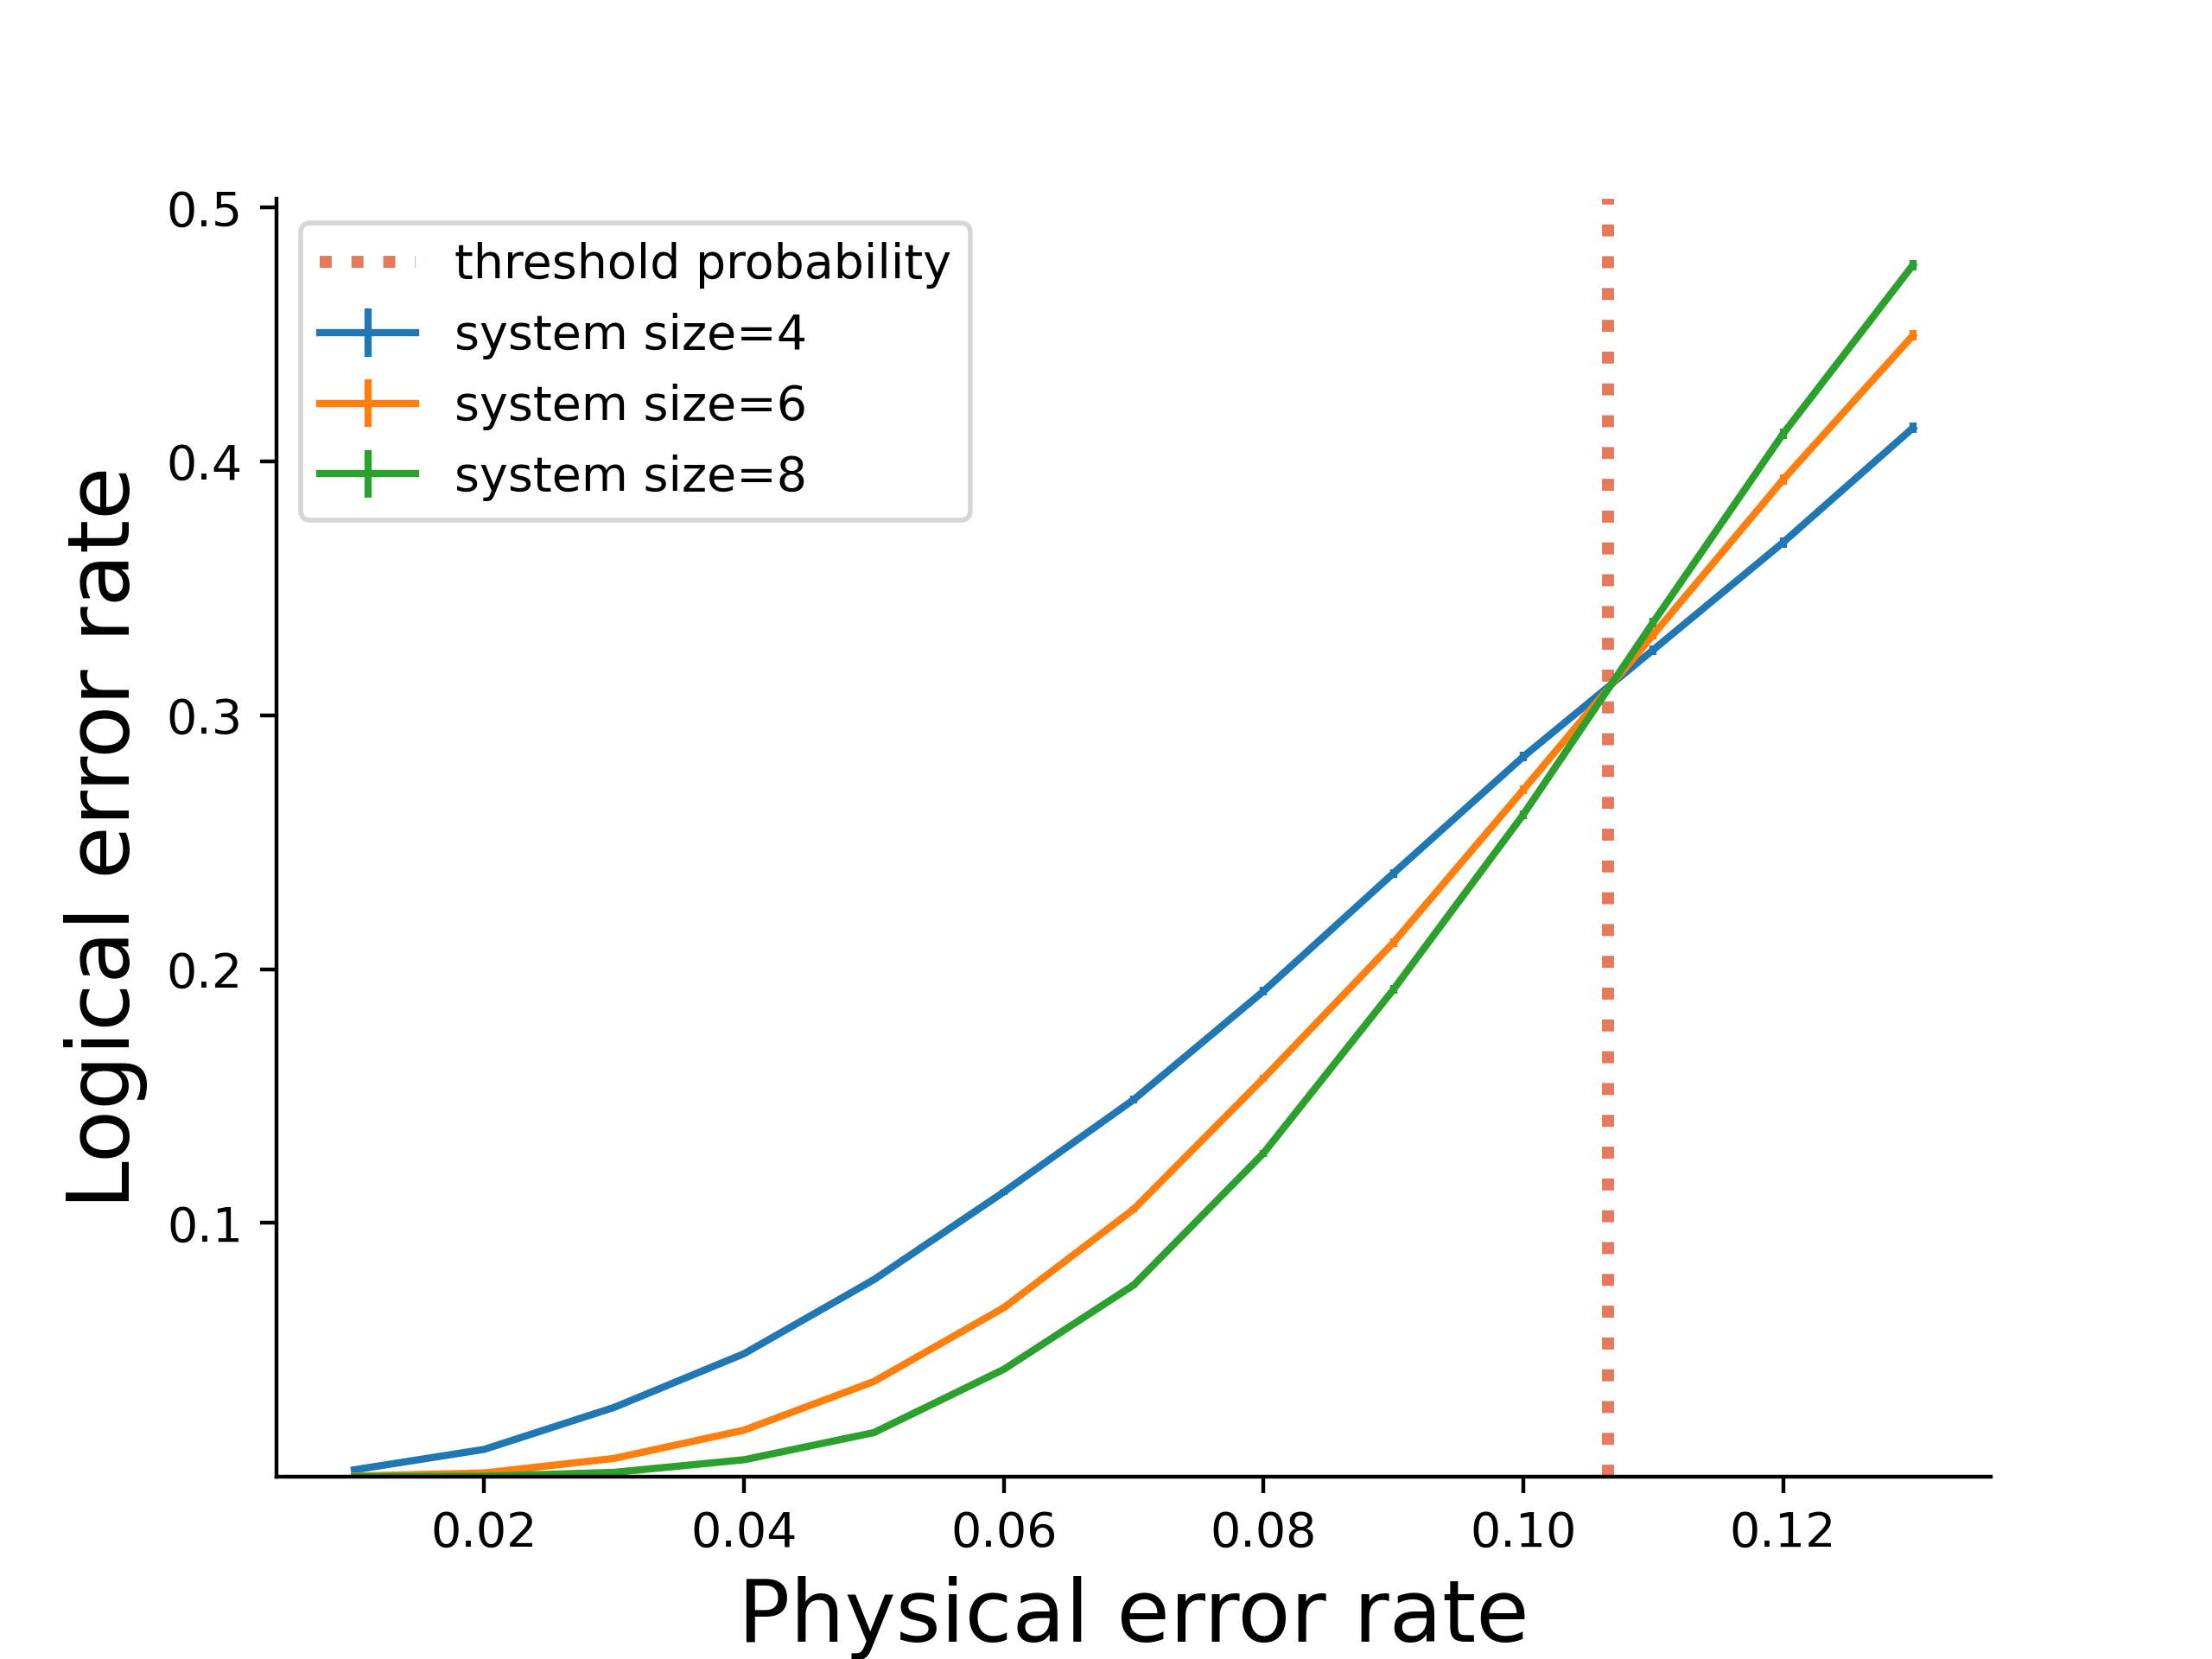
\includegraphics[width=0.5\textwidth]{fig/threshold.png}
	\end{textblock*}
	\begin{textblock*}{8cm}(0.5cm,3cm)
		\textbf{Optimal decoding:}\\
		TN decoder approximates optimal decoding and gives full curves:
		\begin{itemize}
			\item Surface code under depolarising noise~\citeauthoryear{bravyi_efficient_2014}
			\item Surface code under biased Pauli noise~\citeauthoryear{tuckett_ultrahigh_2018}
		\end{itemize}
	\end{textblock*}
	}
\end{frame}

\begin{frame}{Gap}
	Existing:
	\begin{itemize}
		\item Much effort in development of error correcting codes with good quality markers: Number logical per physical qubits, code distance and $p_{\text{threshold}}$
		\item Much effort in development of fast and high performant decoders
	\end{itemize}
	\pause
	Laking:
	\begin{itemize}
		\item Comparibility of codes for finite size regime under realistic noise models
		\item Gauge of existing decoders with respect to optimal code capacity
	\end{itemize}

\end{frame}
\begin{frame}{Research goal}
	Development of hardware adaptive framework:
	\begin{center}
		\raisebox{-0.5cm}{
\includegraphics[width=0.15\textwidth]{fig/Noise.png}}
		\begin{tikzpicture}[overlay]
			\draw[->, line width=0.8mm, black] (0.5, 0.1) -- (4,0.1);
			\draw[-, line width=0.8mm, black] (0.5, 0.3) -- (0.5,-0.1);
		\end{tikzpicture}
		\hspace{4.5cm}
		Optimal code performance estimate
	\end{center}\vspace{20pt}

	\begin{itemize}
		\item Informed decision on which codes promise good finite size performance
		\item Gauge of decoder optimization process
	\end{itemize}
\end{frame}

\begin{frame}{Groundwork for Results - Example}
\textbf{Example:}
\begin{itemize}
	\item Physical errors $E_{1}, E_{2}, E_{3}$ compatible with partial error information\\
	\pause
	\item $E_{2}, E_{3}$ act equivalently on logical qubit (same class) while $E_{1}$ does not\\
	\pause
	\item $P(E_{1})=4\%$, $P(E_{2})=3\%$, $P(E_{3})=3\%$
\end{itemize}
\pause
\vspace{0.5cm}
\textbf{Maximum Probability decoding:}\\
Select most probable physical error consistent with the partial error information\\
\pause
$P(E_{1})\geq P(E_{i})\forall i \Rightarrow$ Select error $E_{1}$\\
\pause
\vspace{0.5cm}
\textbf{Maximum likelihood/Optimal decoding:}\\
Select most probable error class consistent with the partial error information\\
\pause
$P([E_{2}])=P(E_{2})+P(E_{3})> P(E_{1})\Rightarrow$ Select error class $[E_{2}]=[E_{3}]$
\end{frame}

\begin{frame}{Groundwork for Results - Decoder}
	\only<1-1>{
	\textbf{Maximum Probability decoding:}\\
	Select error consistent with the partial error information and highest $P(E)$\\
	}
	\pause
	\only<2-3>{
	\textbf{Maximum Probability/Minimum Weight decoding:}\\
	Select error consistent with the partial error information and highest $P(E)$\\
	}
	\pause
	\only<3-3>{
	\vspace{0.5cm}
	\textbf{Maximum likelihood/Optimal decoding:}\\
	Select class consistent with the partial error information and highest $P([E])$
	}
	\pause
	\only<4-4>{
		\textbf{Statistical mechanics mapping~\citeauthoryear{dennis_topological_2002}:}\\
		Reduce calculation of $P(E)$ and $P([E])$ to very well studied partition function $Z_{E}(T)$ calculation\\
	}
	\pause
	\only<5-5>{
		\textbf{Maximum Probability/Minimum Weight decoding:}\\
		Select error consistent with the partial error information and highest $P(E)=lim_{T\to 0}Z_{E}(T)$\\
		\vspace{0.5cm}
		\textbf{Maximum likelihood/Optimal decoding:}\\
		Select class consistent with the partial error information and highest $P([E])=Z_{E}(T_{\text{Nishimori}})$
	}
\end{frame}

\begin{frame}{Groundwork for Results - Success Rates}
	Brute force simulation of decoding sample intensive $\rightarrow$ Define efficient estimators\\
	\pause
	\vspace{0.5cm}
	\textbf{Maximum Probability/Minimum Weight decoding:}\\
	Succees rate estimator: Order probability~\citeauthoryear{thomas_simplest_2011}\\
	\pause
	\vspace{0.5cm}
	\textbf{Maximum likelihood/Optimal decoding:}\\
	We introduce success rate estimator: Decoding probability
	\pause
	\begin{tcolorbox}[colback=osakared!5!white, colframe=osakared, width=13cm, arc=2mm]
		\textbf{General framework:}\\ Relies only on mapping of error correcting code $+$ noise to statistical mechanics system.
	\end{tcolorbox}
\end{frame}

\begin{frame}{Results}
	\only<1-1>{
	\begin{textblock*}{14cm}(1.5cm,2cm)
		\raisebox{-0.5cm}{
\includegraphics[width=0.15\textwidth]{fig/Noise.png}}
		\begin{tikzpicture}[overlay]
			\draw[->, line width=0.8mm, black] (0.5, 0.1) -- (4,0.1);
			\draw[-, line width=0.8mm, black] (0.5, 0.3) -- (0.5,-0.1);
		\end{tikzpicture}
		\hspace{4.5cm}
		Optimal code performance estimates
	\end{textblock*}
	}
	\pause
	\only<2->{
		\vspace{2cm}
		\hspace{1.5cm}
		\begin{itemize}
			\item Minimum weight decoding $\sim$ order probability
			\item Optimal decoding $\sim$ decoding probability
		\end{itemize}
		\begin{textblock*}{14cm}(1.5cm,2cm)
			\raisebox{-0.7cm}{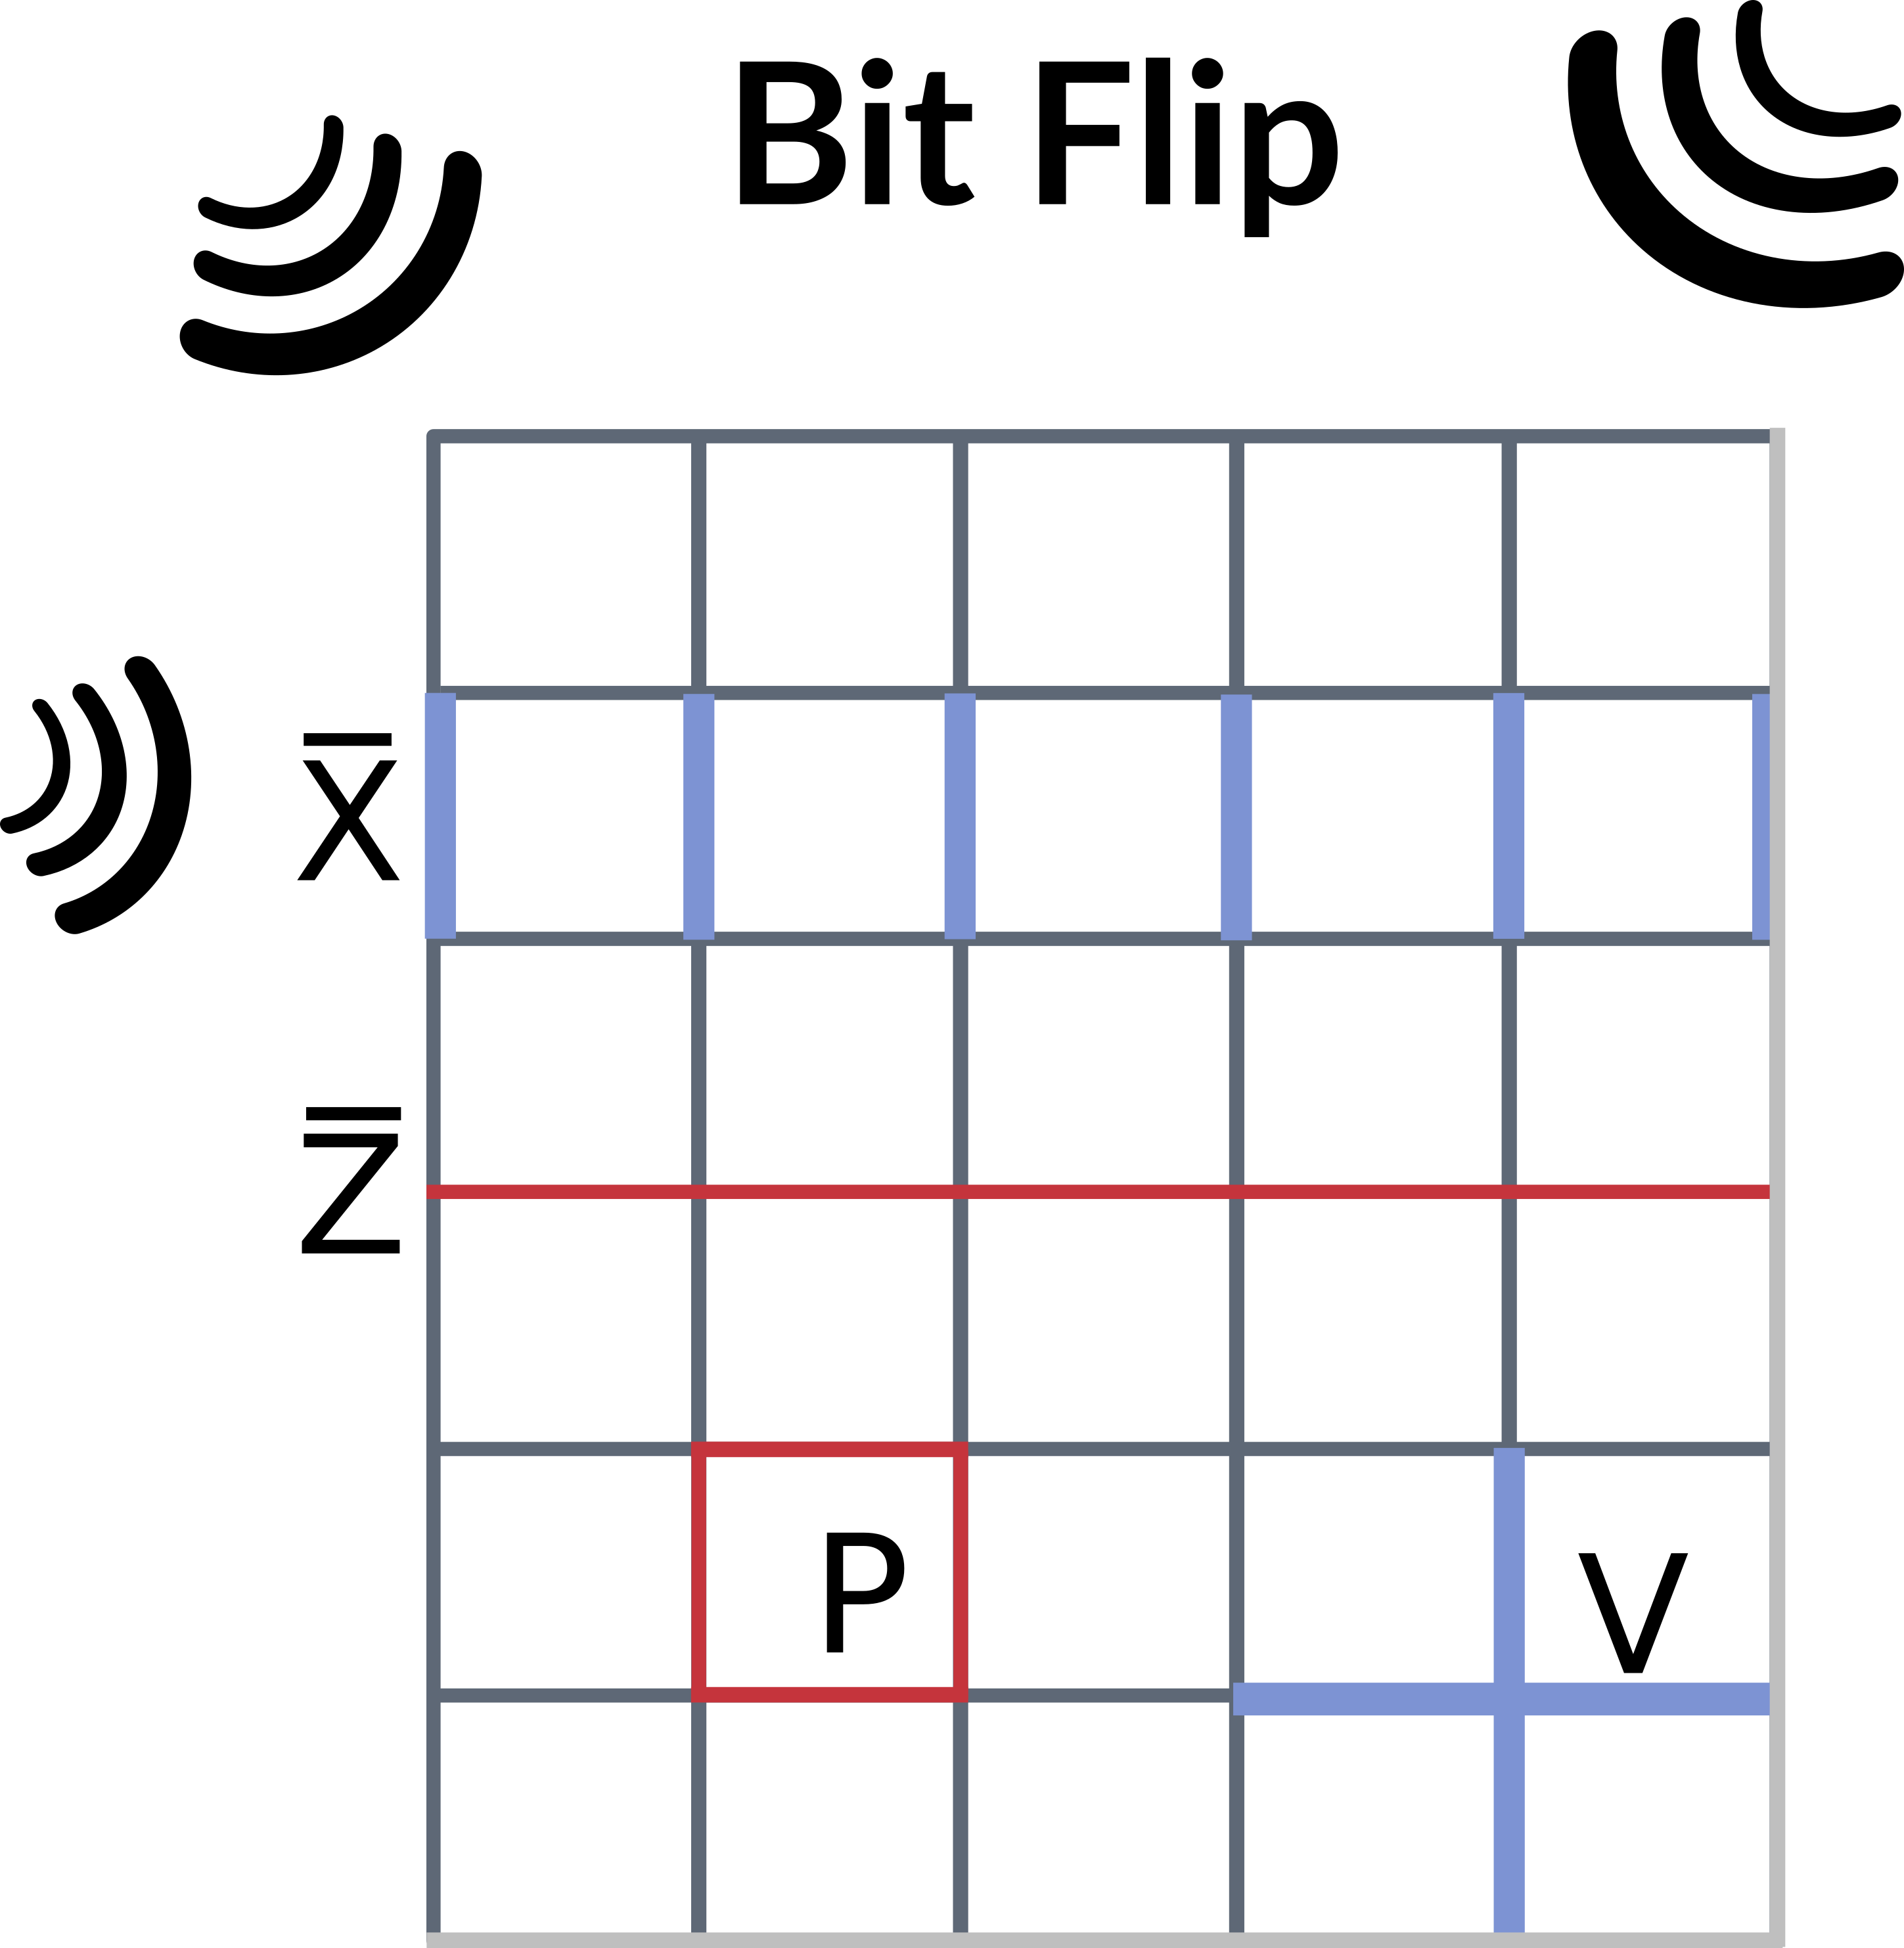
\includegraphics[width=0.15\textwidth]{fig/toric_code.png}}
			\begin{tikzpicture}[overlay]
				\draw[->, line width=0.8mm, black] (0.5, 0.1) -- (4,0.1);
				\draw[-, line width=0.8mm, black] (0.5, 0.3) -- (0.5,-0.1);
			\end{tikzpicture}
			\hspace{4.5cm}
			Error class probability estimates
		\end{textblock*}
	}
\end{frame}

\begin{frame}{Results - Zero T Limit}
	\textbf{Theoretical MP/MW decoding:}\\
	Select error consistent with the partial error information and highest $P(E)=lim_{T\to 0}Z_{E}(T)$\\
	\pause
	\vspace{0.5cm}
	\textbf{Numerically:} \\
	REWL~\cite{vogel_generic_2013, wang_efficient_2001} - can take limit but slow\\
	FKT~\cite{kasteleyn_statistics_1961, temperley_dimer_1961, thomas_exact_2009, thomas_numerically_2013} - only finite T but fast\\
	\pause
	\begin{tcolorbox}[colback=osakared!5!white, colframe=osakared, width=13cm, arc=2mm]
		Showed FKT decoding at low $T\neq 0$ approximates WL $T=0$ decoding, e.g. MW decoding
	\end{tcolorbox}
\end{frame}

\begin{frame}{Results - Zero T Limit}
	\only<1->{
	\begin{textblock*}{7.5cm}(0.5cm,3cm)
		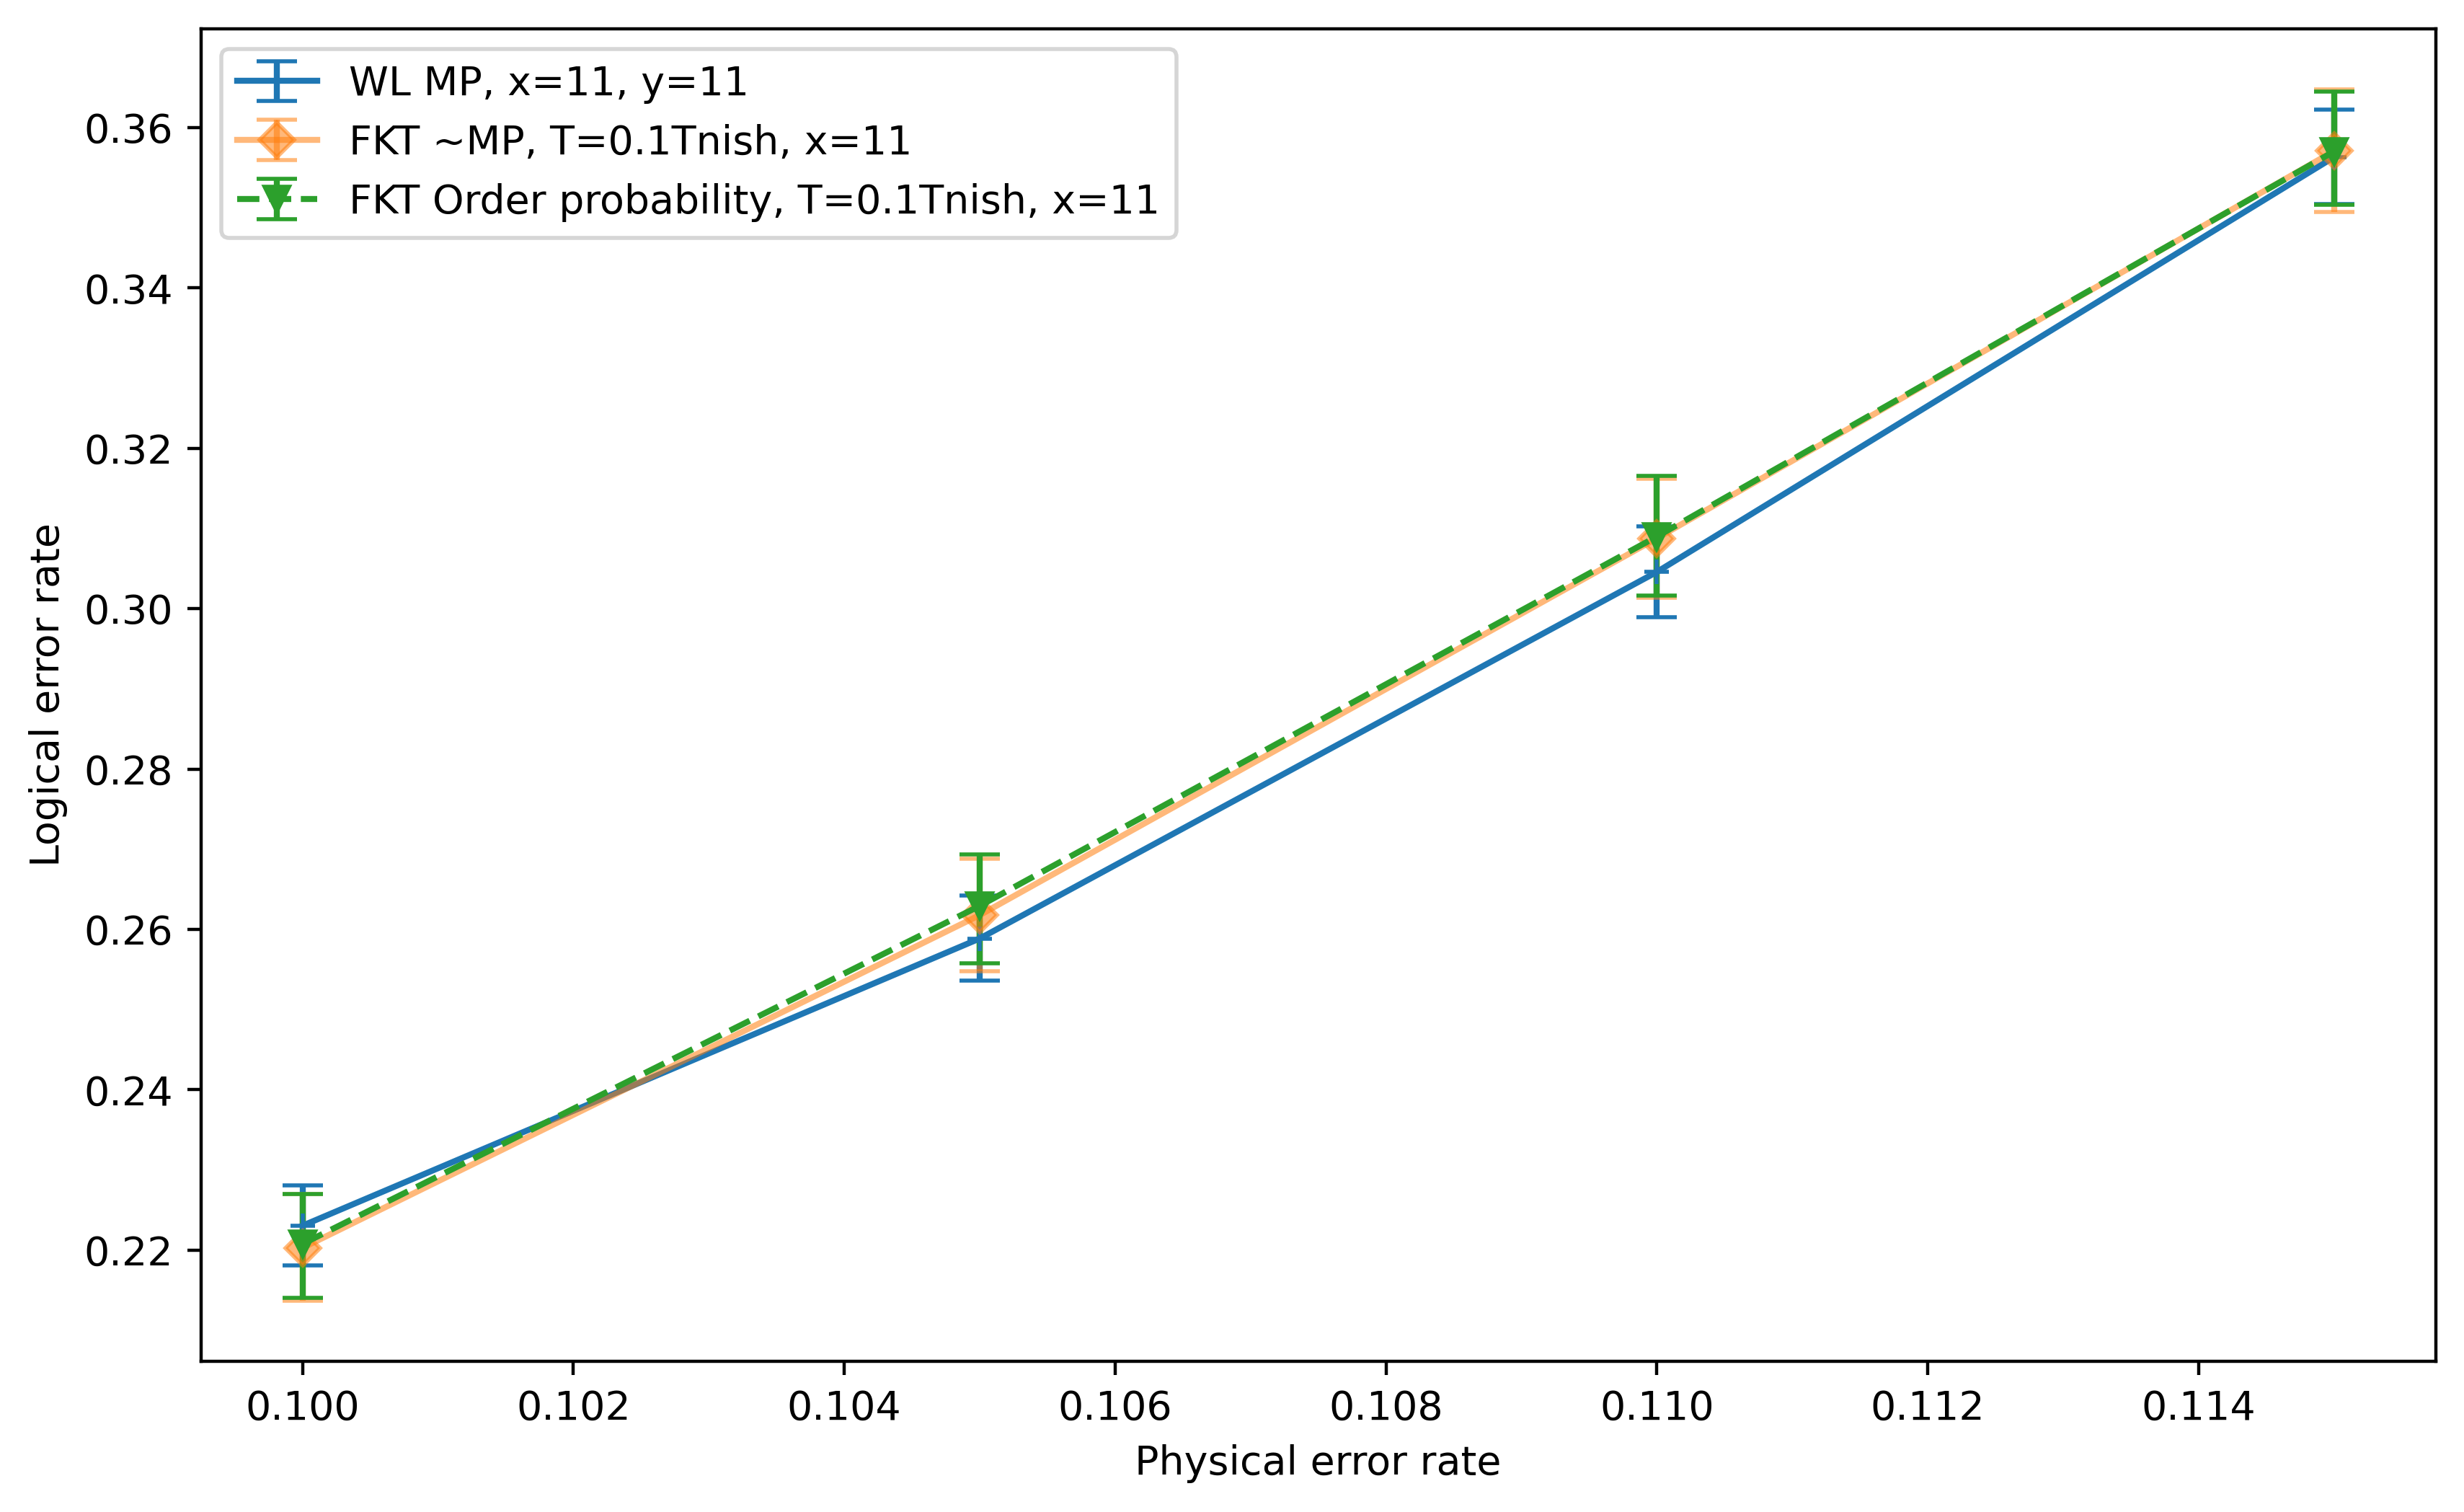
\includegraphics[width=\textwidth]{fig/FKTApproximateMP_WLMP_x11.png}
	\end{textblock*}
	}
	\only<2-2>{
	\begin{textblock*}{7.5cm}(8cm,3cm)
		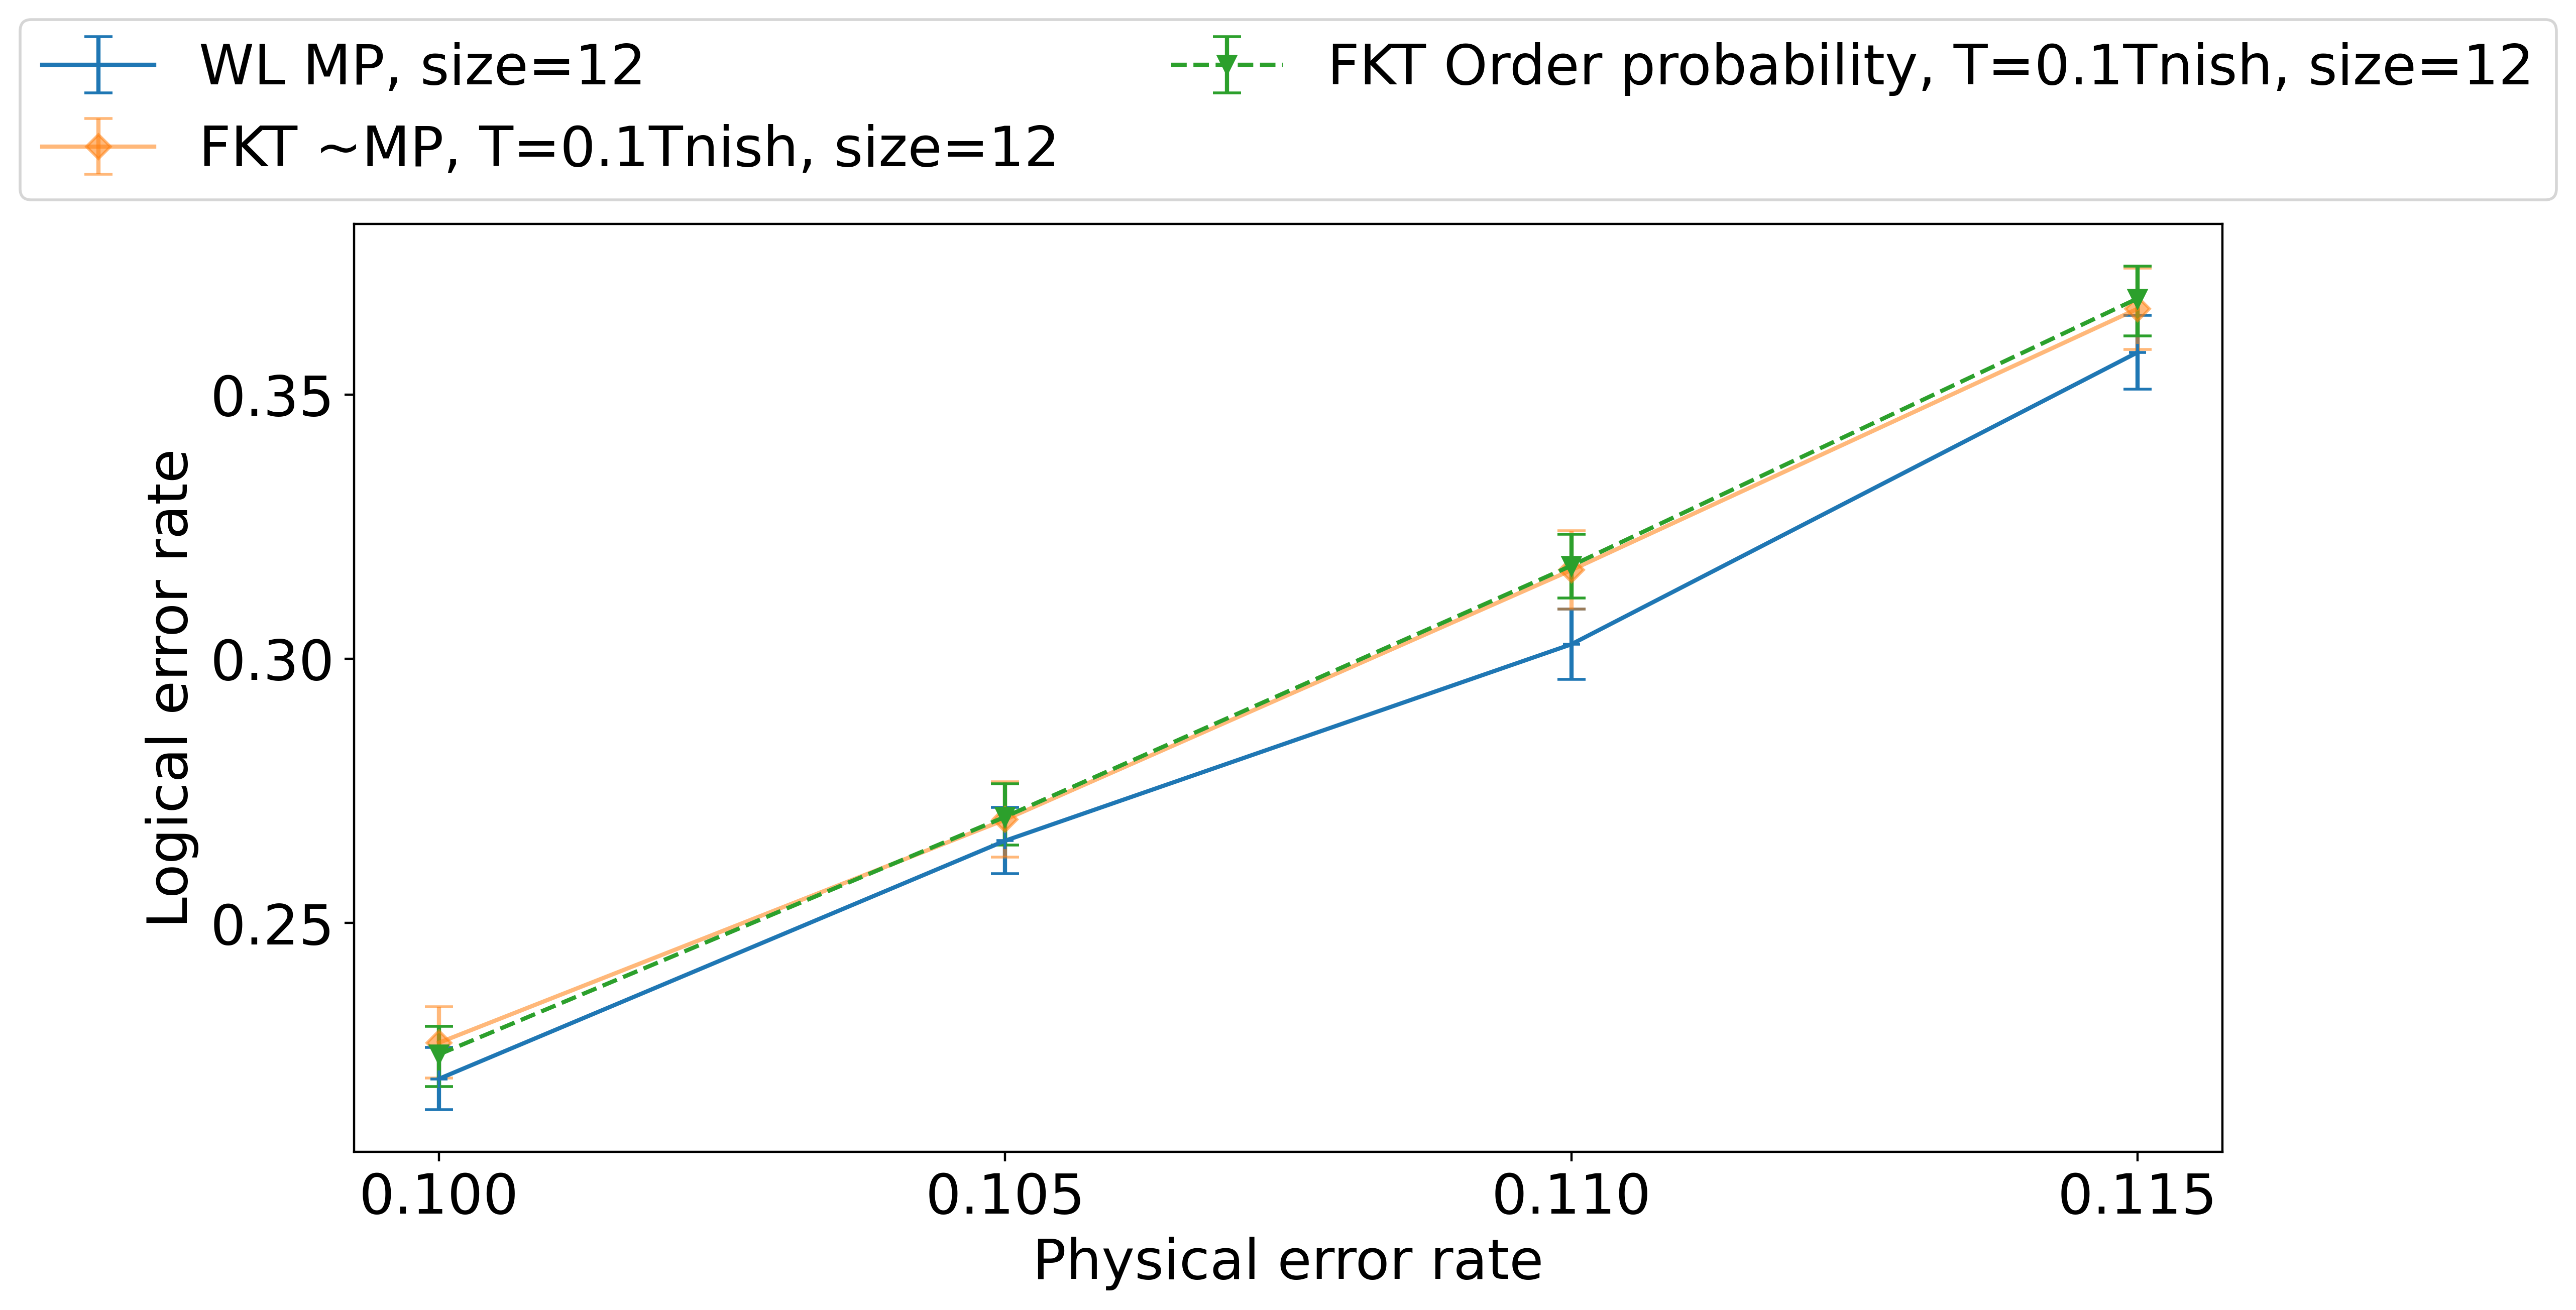
\includegraphics[width=\textwidth]{fig/FKTApproximateMP_WLMP_x12.png}
	\end{textblock*}
	}
\end{frame}

\begin{frame}{Results - Efficient Success Estimation}
	\only<1-2>{
		\begin{textblock*}{7.5cm}(0.5cm,3cm)
			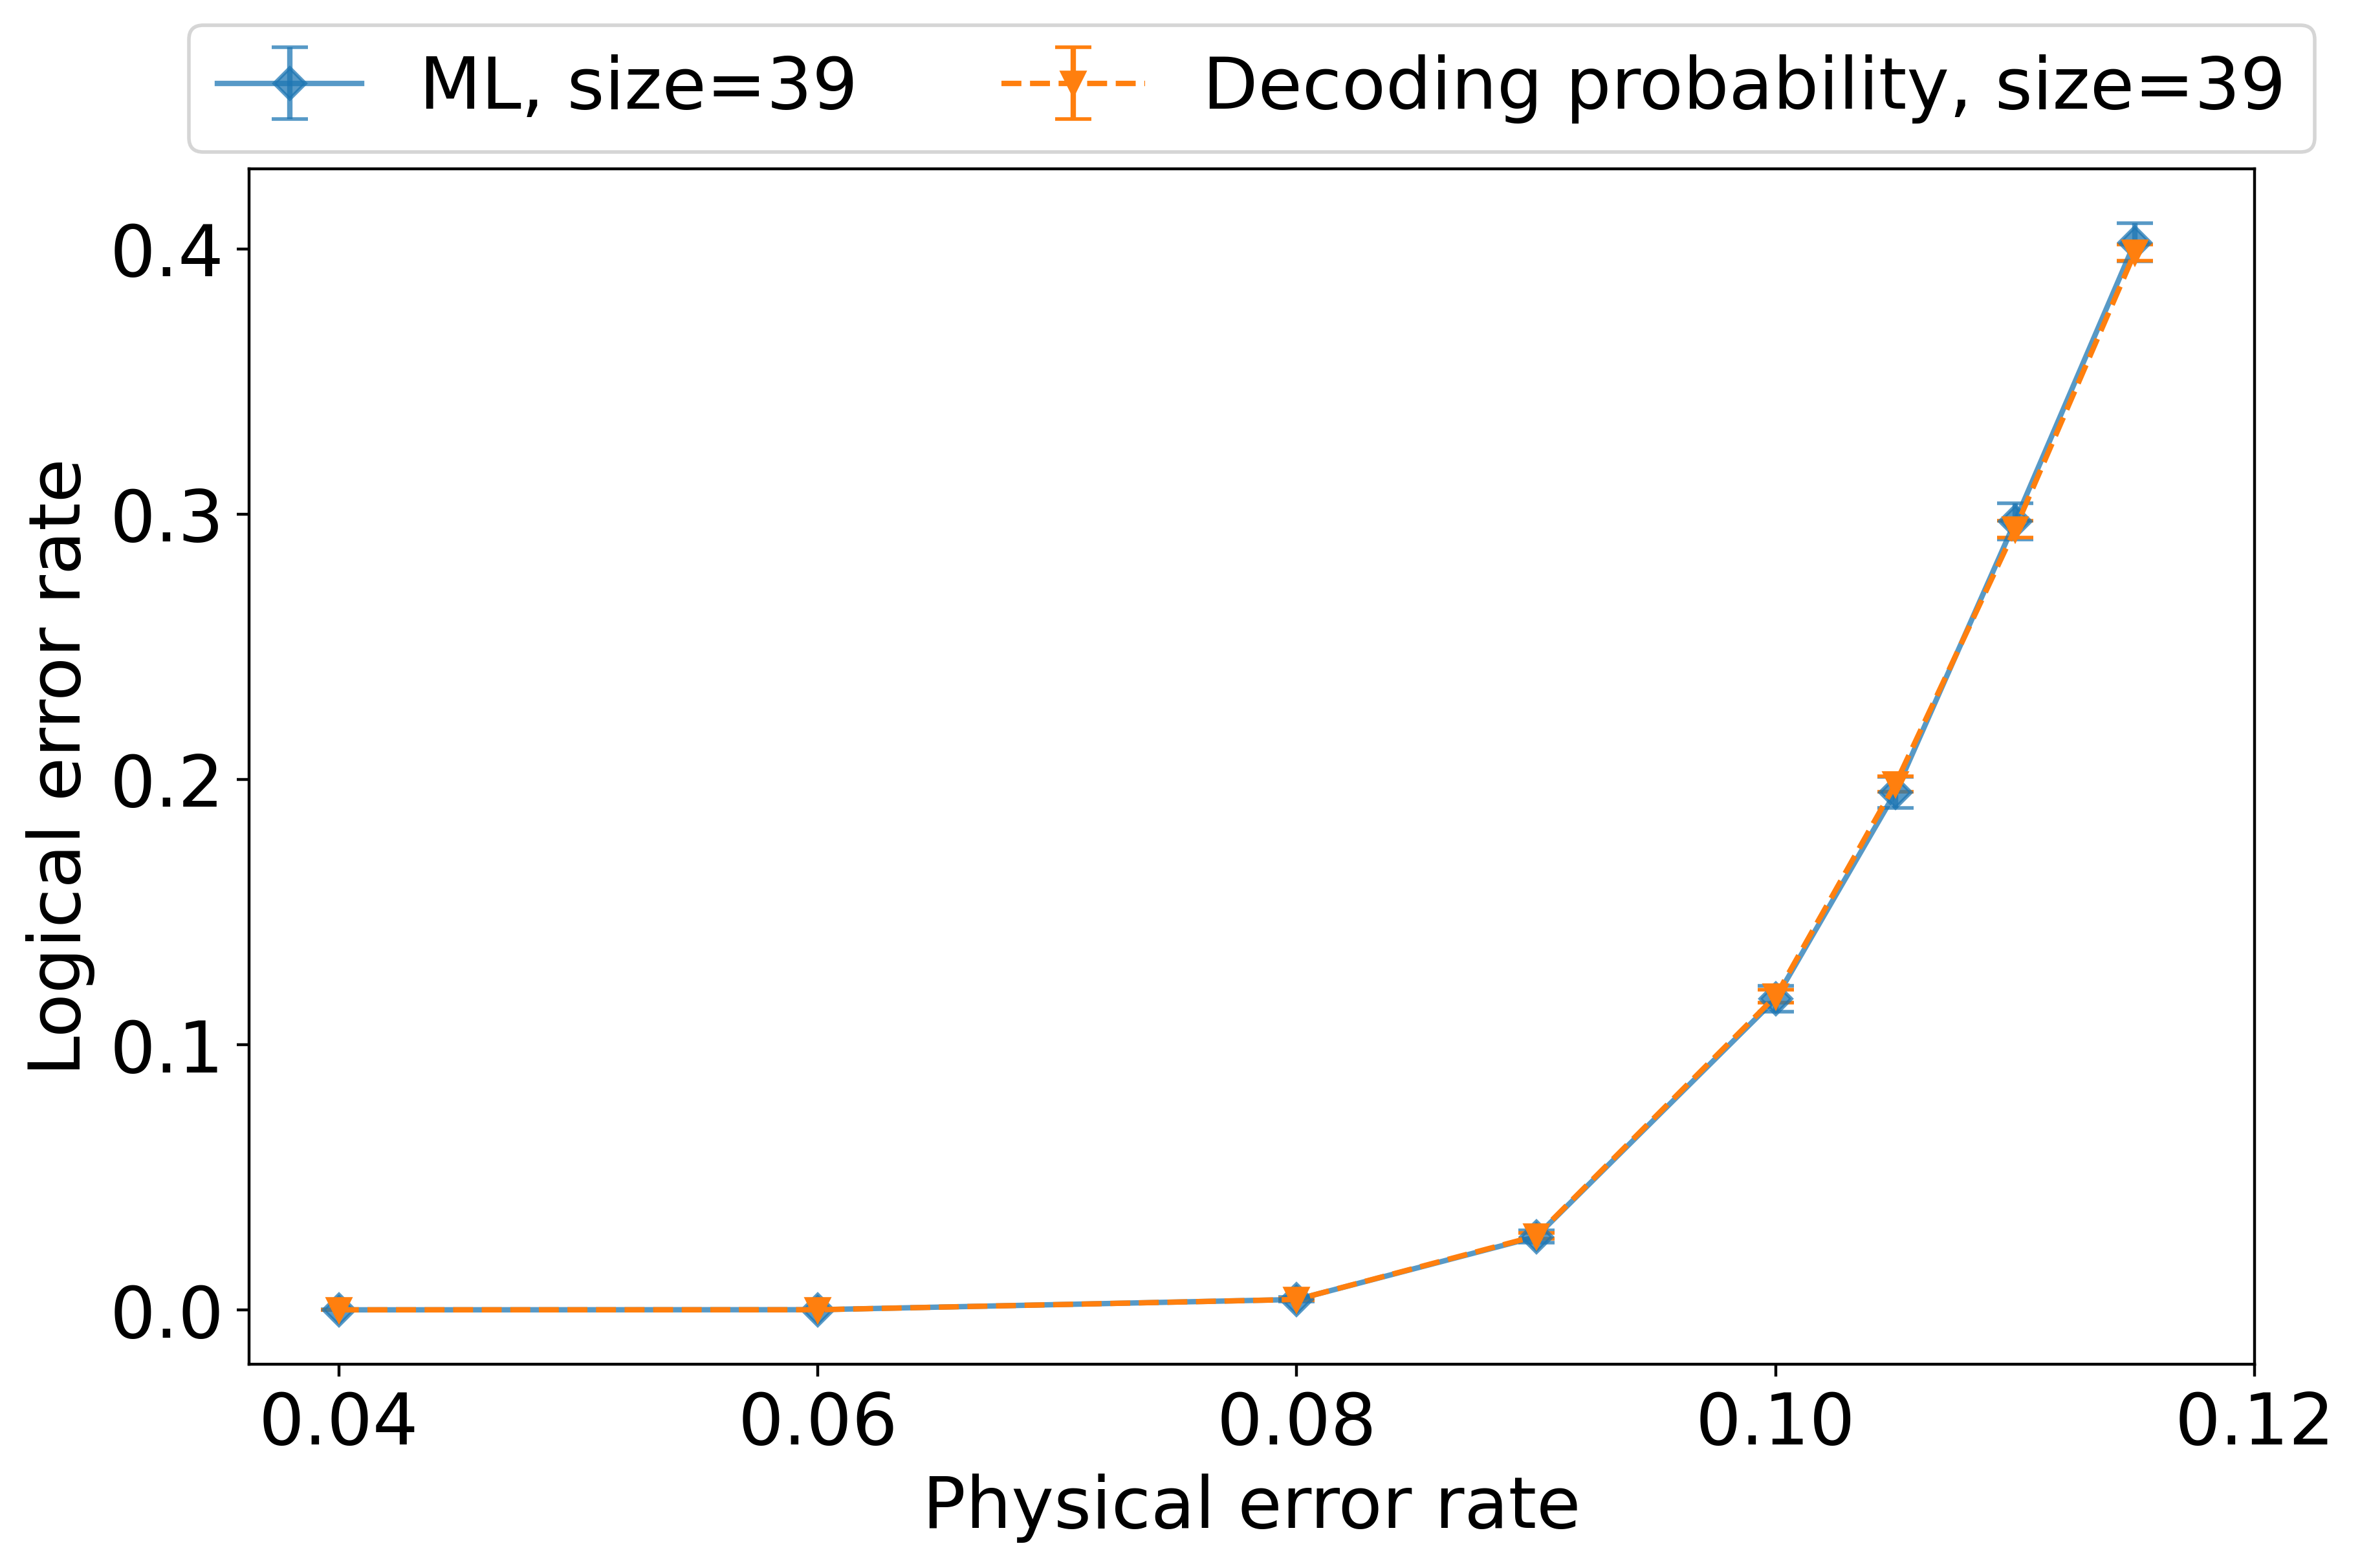
\includegraphics[width=\textwidth]{fig/ML_vs_DecProb_39.png}
		\end{textblock*}
		}
	\only<2->{
		\begin{textblock*}{7.5cm}(8cm,3cm)
			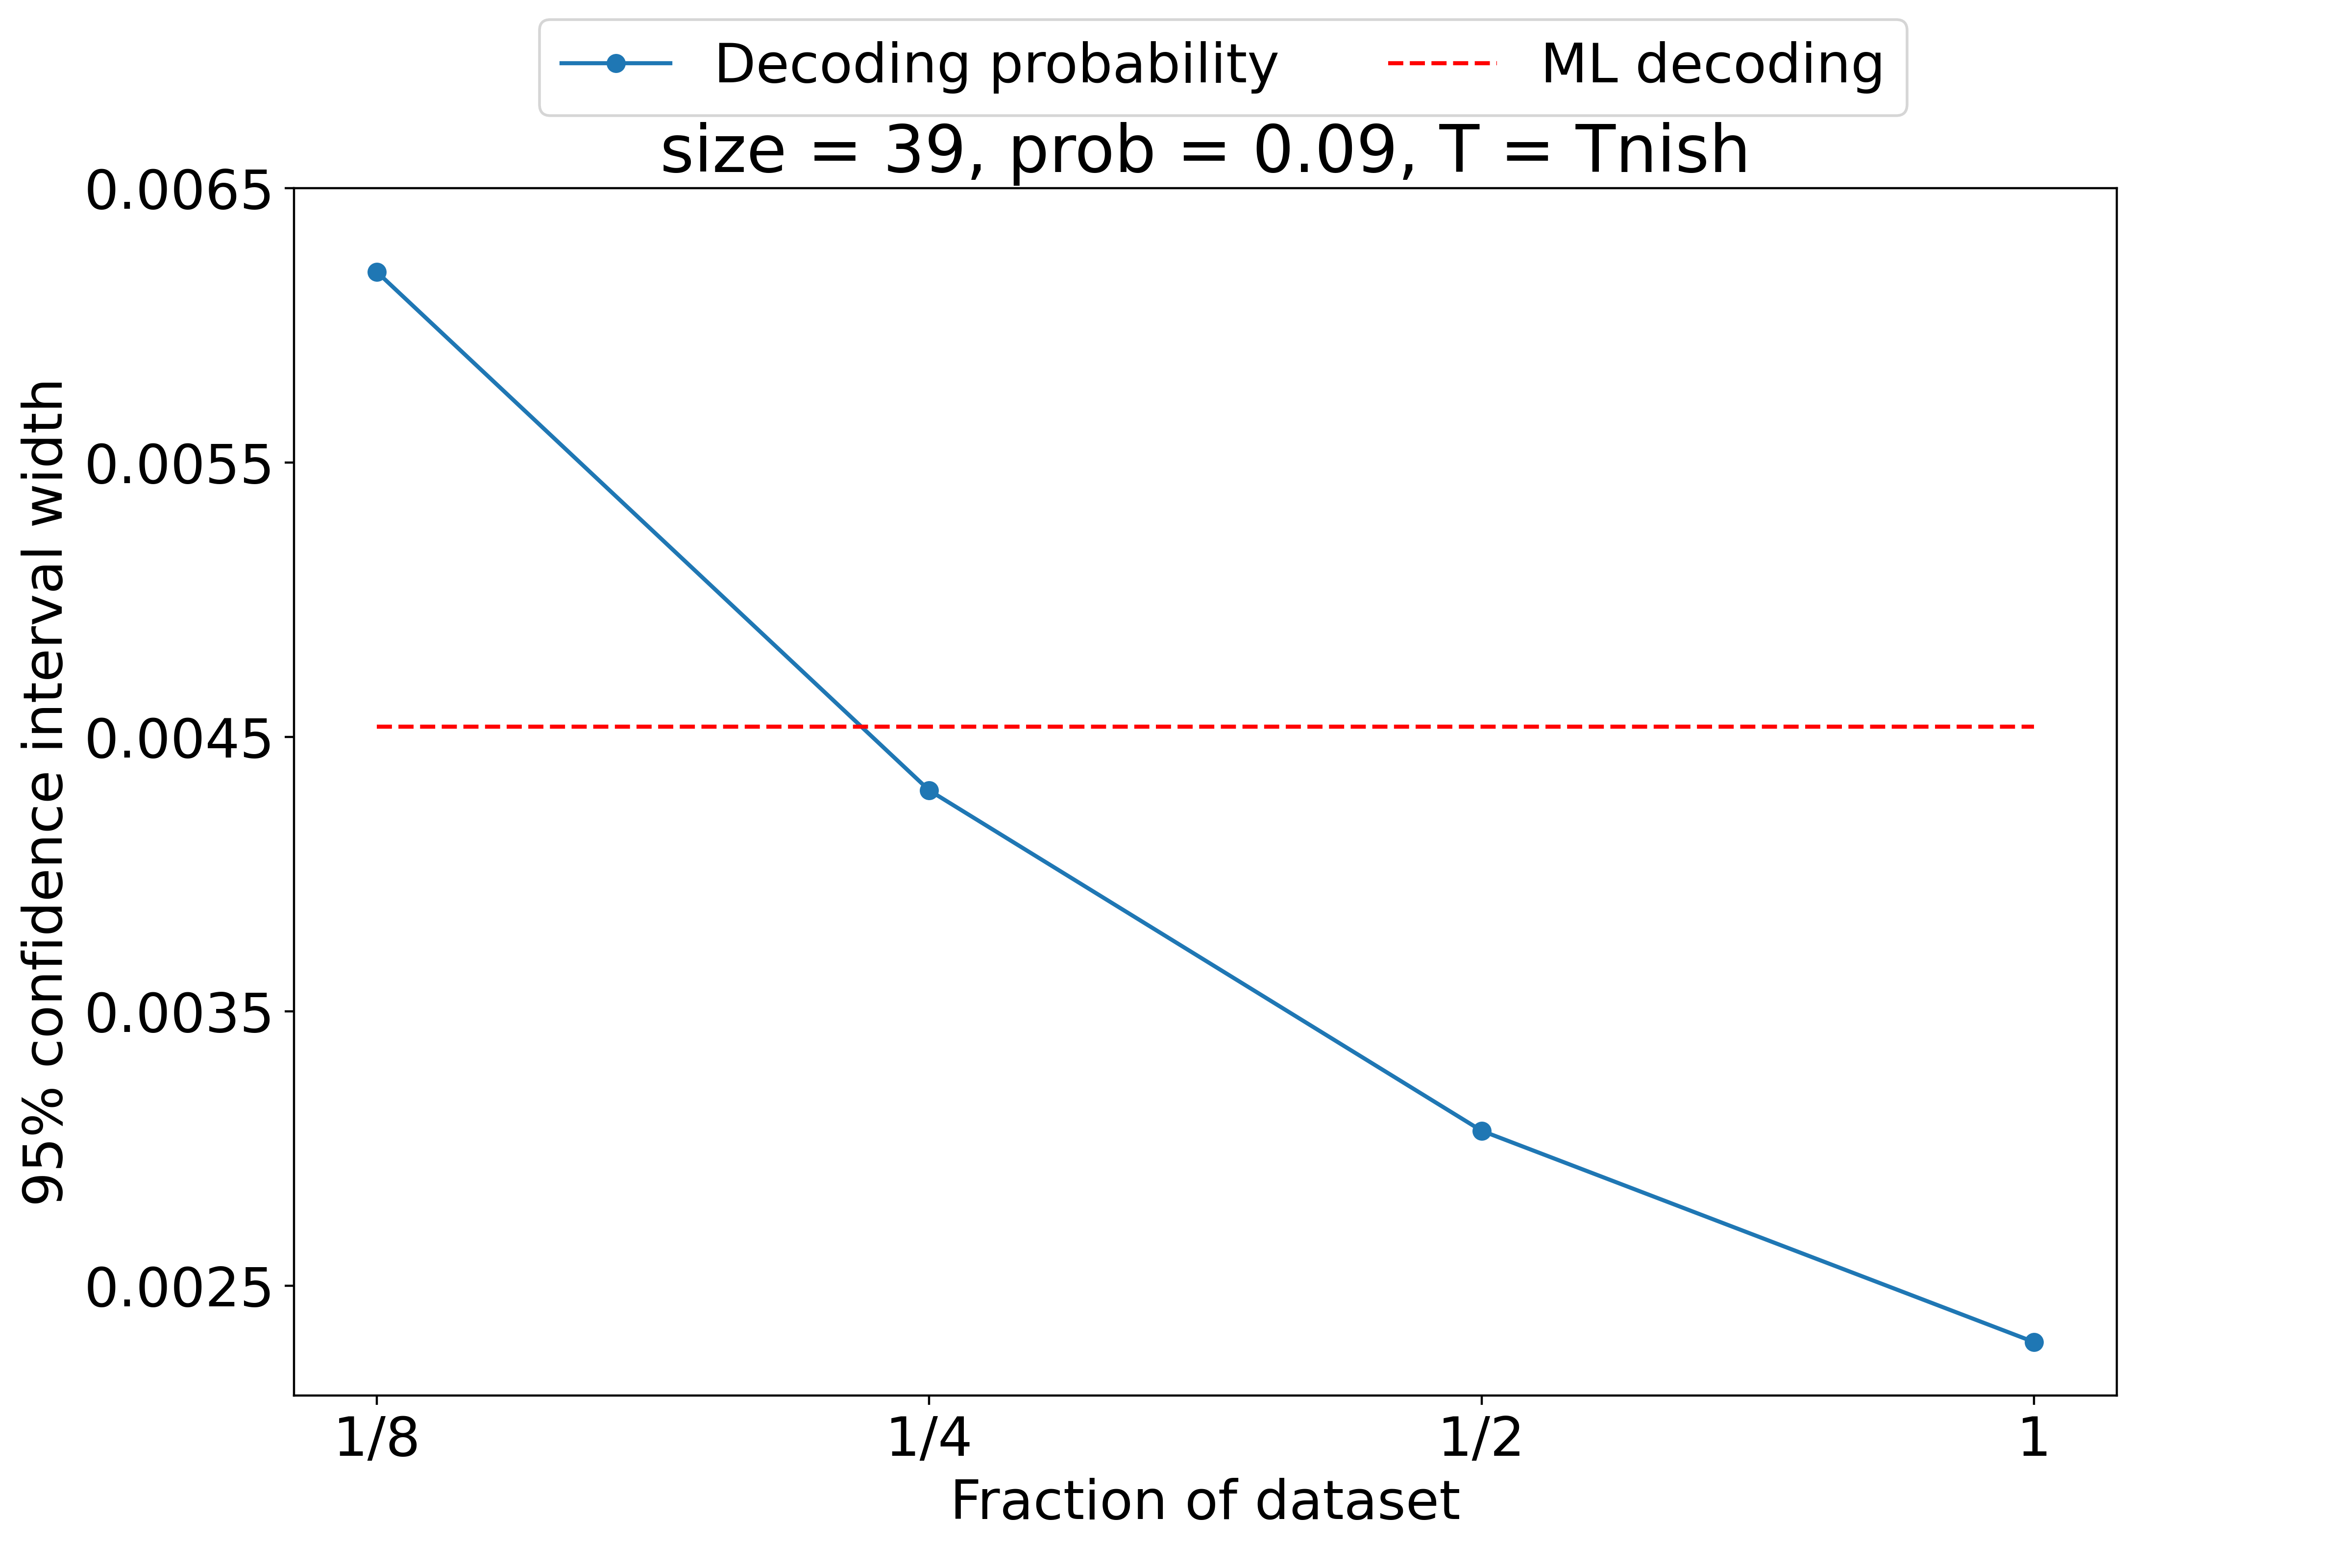
\includegraphics[width=\textwidth]{fig/CIwidth_39.png}
		\end{textblock*}
		}
	\only<3->{
		\begin{textblock*}{7.5cm}(0.5cm,3cm)
			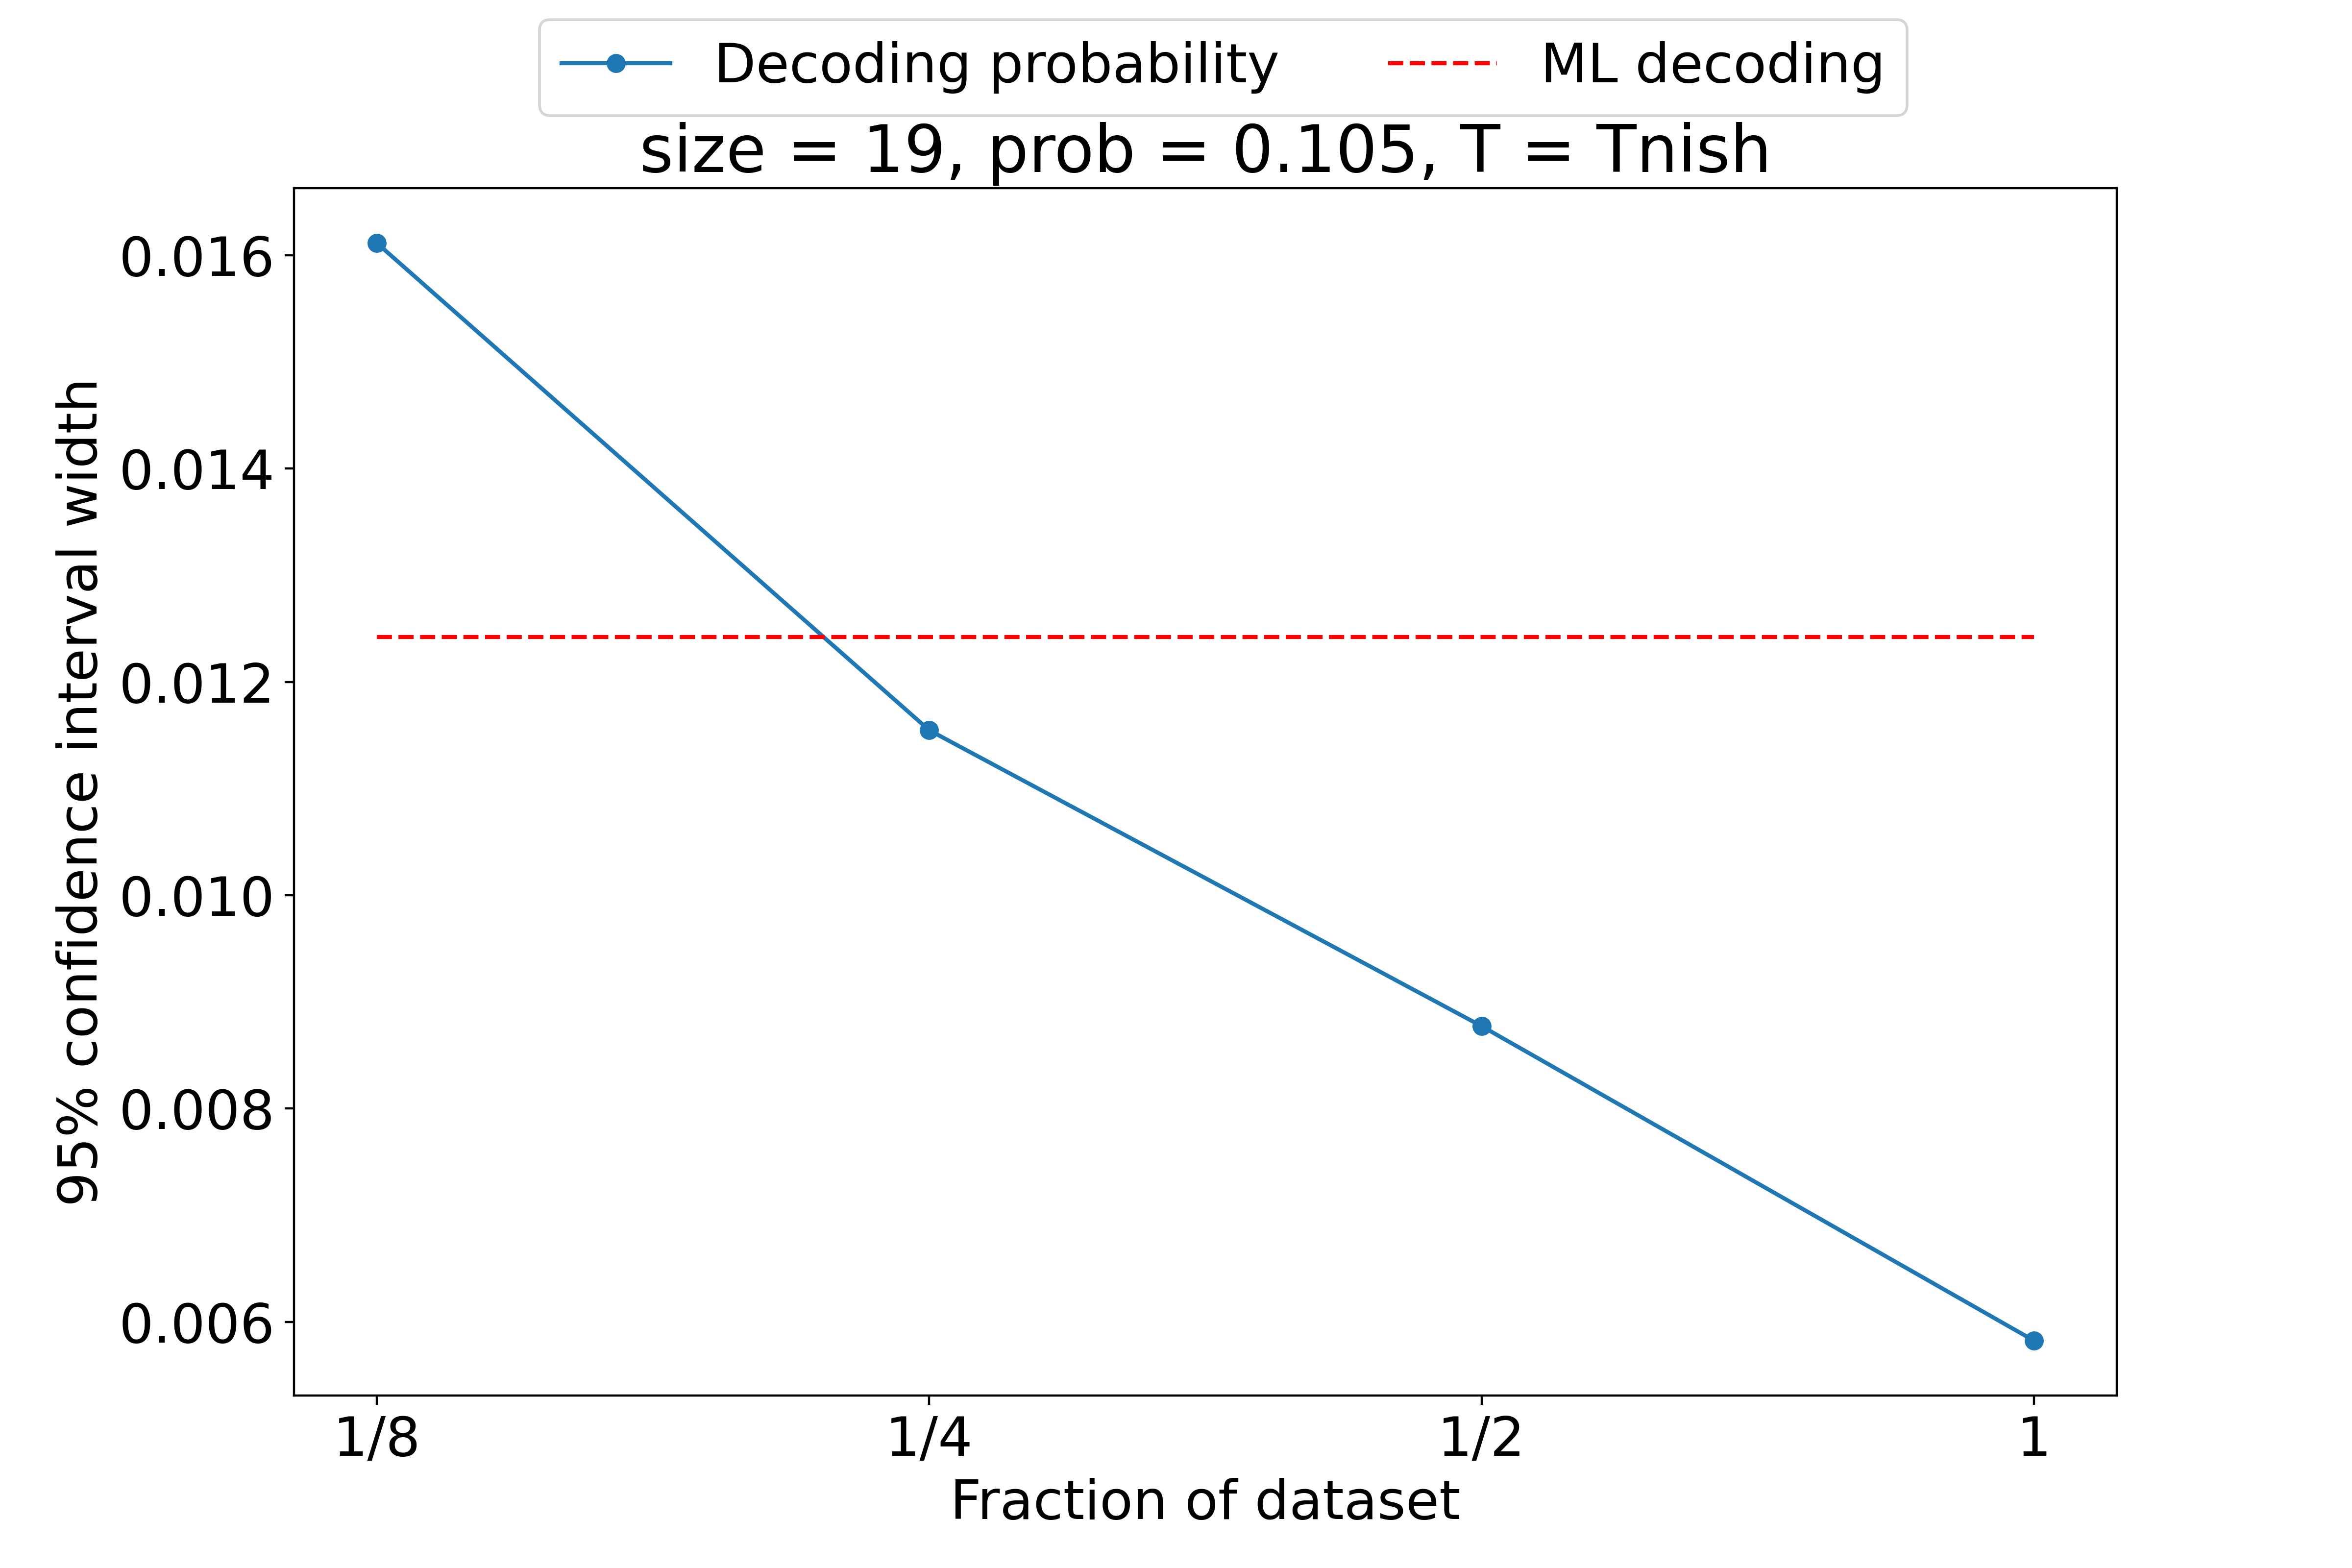
\includegraphics[width=\textwidth]{fig/CIwidth.png}
		\end{textblock*}
		}
\end{frame}

\begin{frame}{Results - MP vs Optimal}
	\only<1-1>{
		\begin{textblock*}{7.5cm}(0.5cm,2.5cm)
			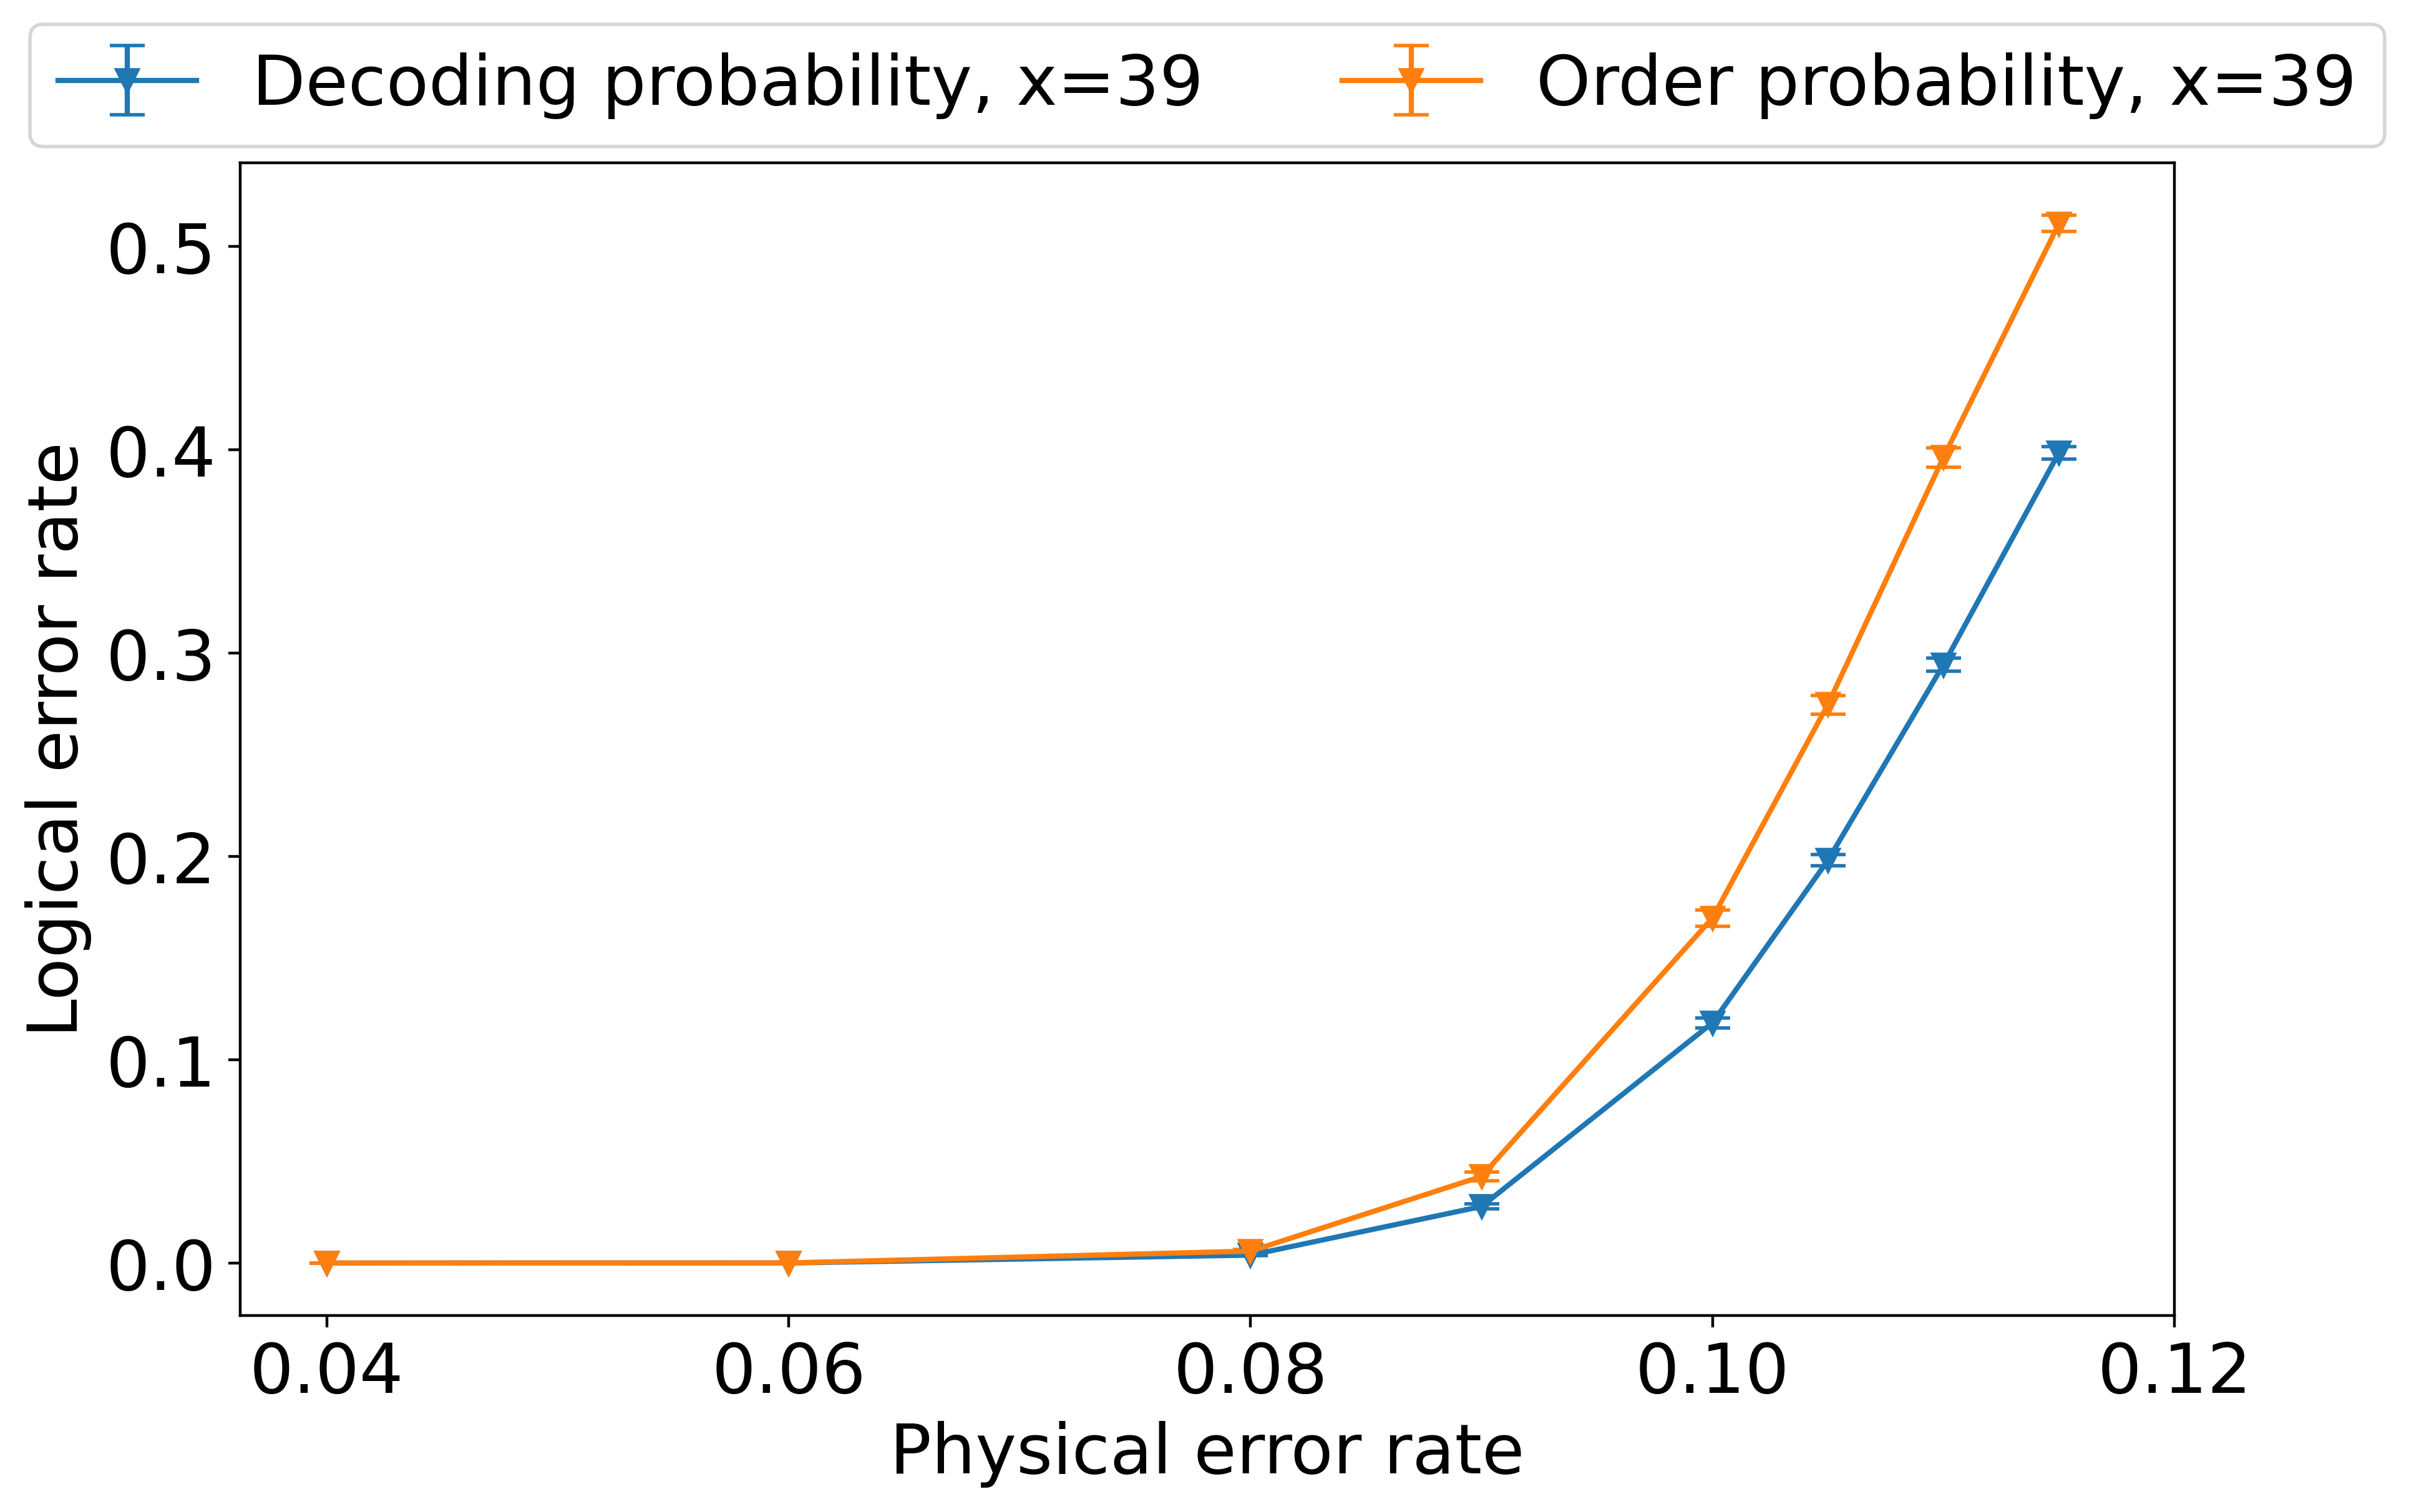
\includegraphics[width=\textwidth]{fig/MP_vs_ML_39.png}
		\end{textblock*}
	}
	\only<2->{
		\begin{textblock*}{7.5cm}(0.5cm,2.5cm)
			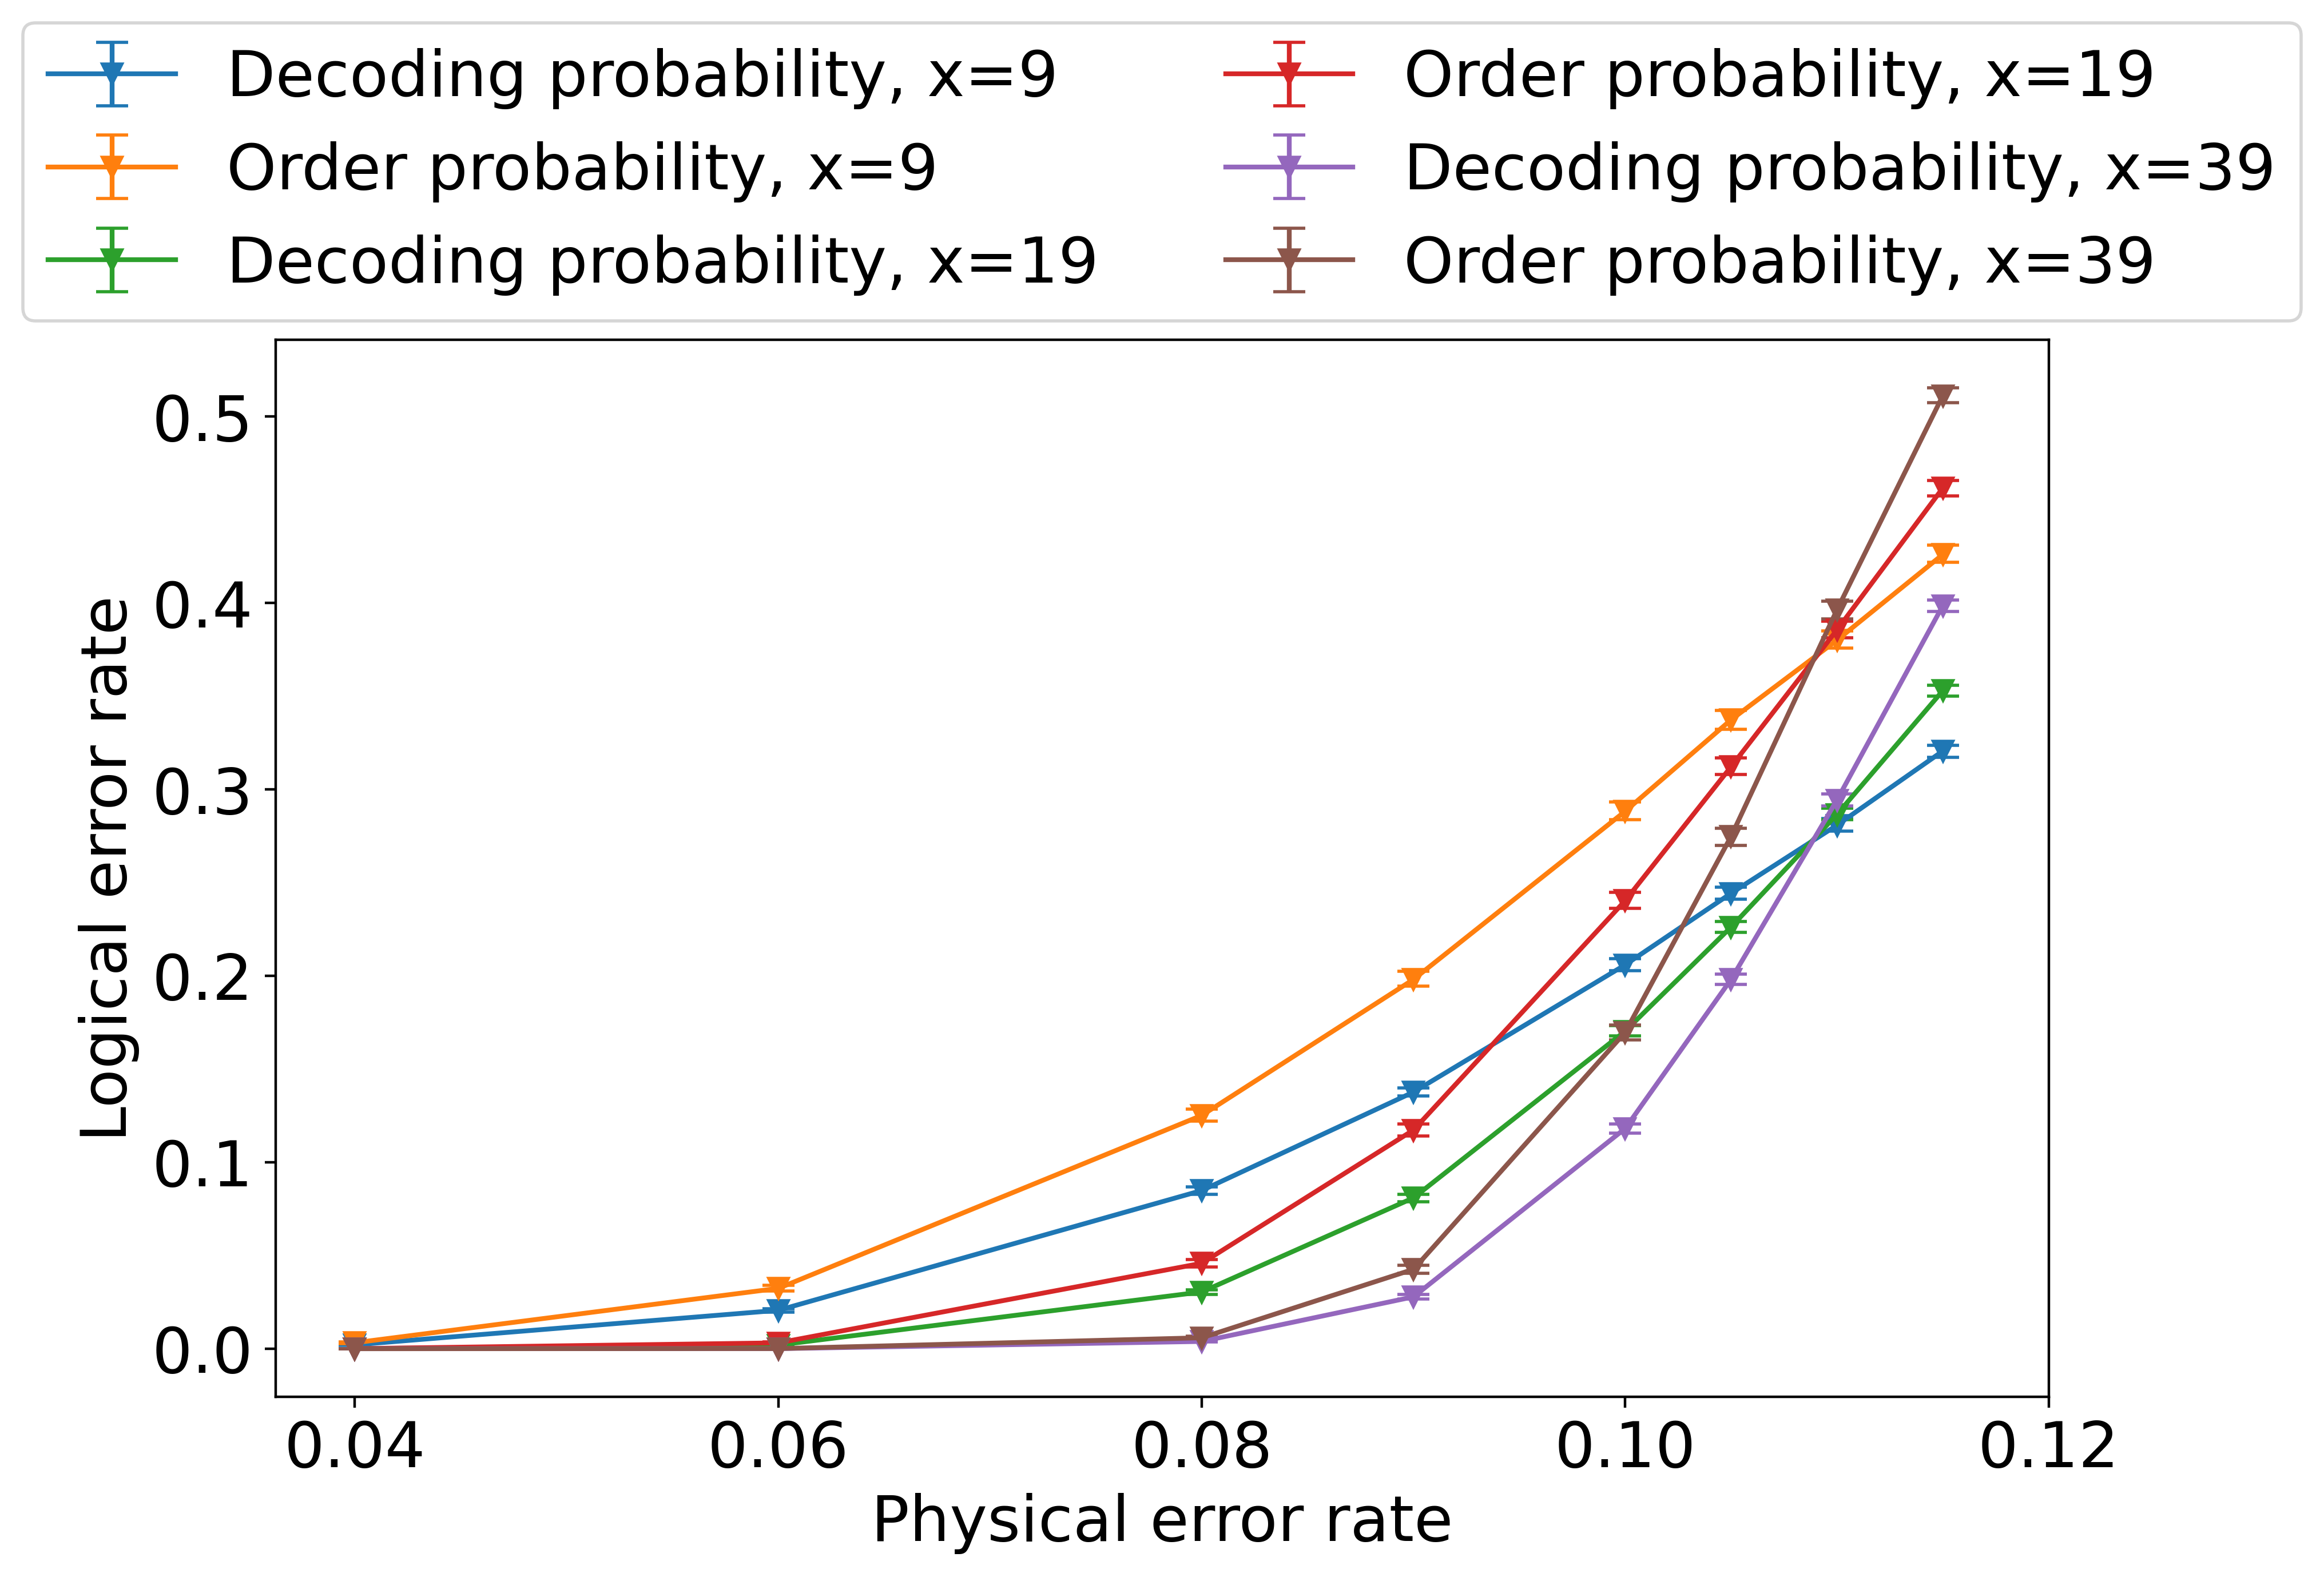
\includegraphics[width=\textwidth]{fig/MP_vs_ML_odd.png}
		\end{textblock*}
	}
	\only<3->{
	\begin{textblock*}{7.5cm}(8cm,2.5cm)
		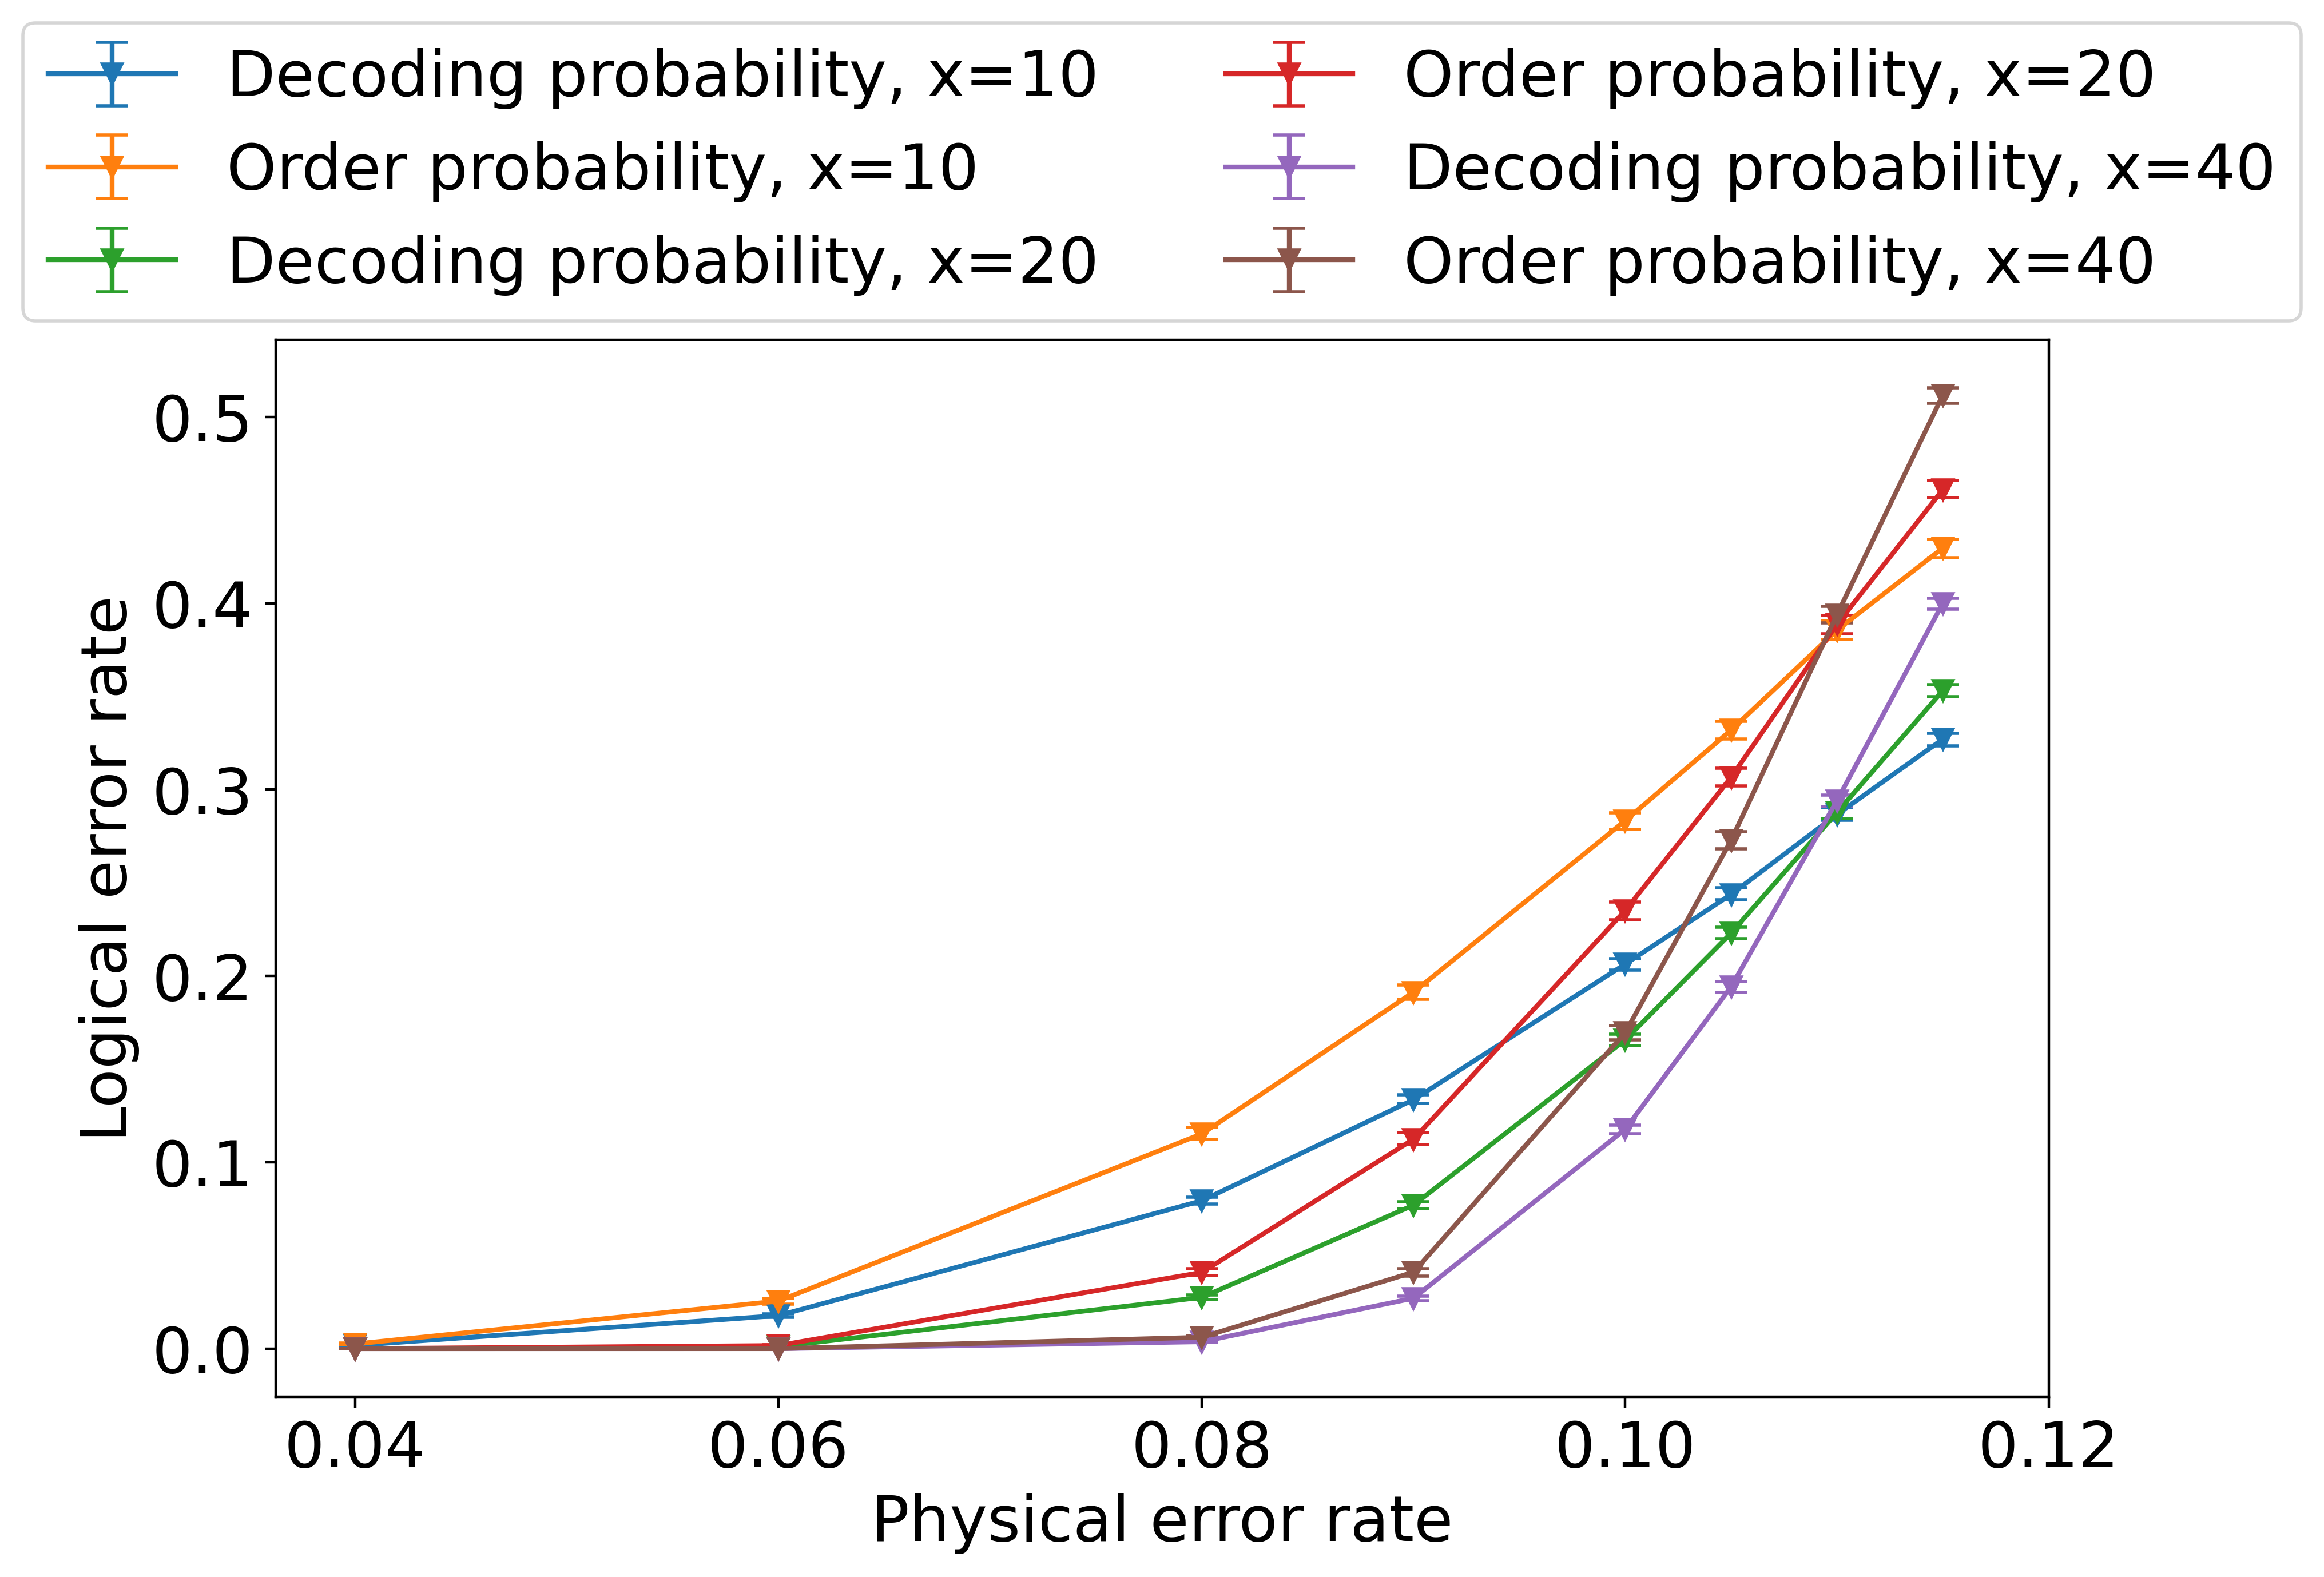
\includegraphics[width=\textwidth]{fig/MP_vs_ML_even.png}
	\end{textblock*}
	}
\end{frame}

\begin{frame}{Results - Improving MP/MW}
	\textbf{Example:}
	\begin{itemize}
		\item Physical errors $E_{1}, E_{2}, E_{3}$ compatible with partial error information\\
		\pause
		\item $E_{2}, E_{3}$ act equivalently on logical qubit (same class) while $E_{1}$ does not\\
		\pause
		\item $P(E_{1})=4\%$, $P(E_{2})=4\%$, $P(E_{3})=4\%$
	\end{itemize}
	\pause
	\textbf{MP/MW Decoding:}\\
	Select most probable physical error consistent with the partial error information\\
	$\Leftrightarrow$ Select randomly under most probable errors\\
	\pause
	Use knowledge on how many maximum probability errors are within different error classes:\\
	\textbf{Degeneracy Enhanced MP Decoding:}\\
	Select error class with highest degeneracy of lowest weight errors\\
\end{frame}

\begin{frame}{Results - MP vs dMP}
	\begin{figure}[h!]
		\centering
		\begin{minipage}{0.45\textwidth}
			\centering
			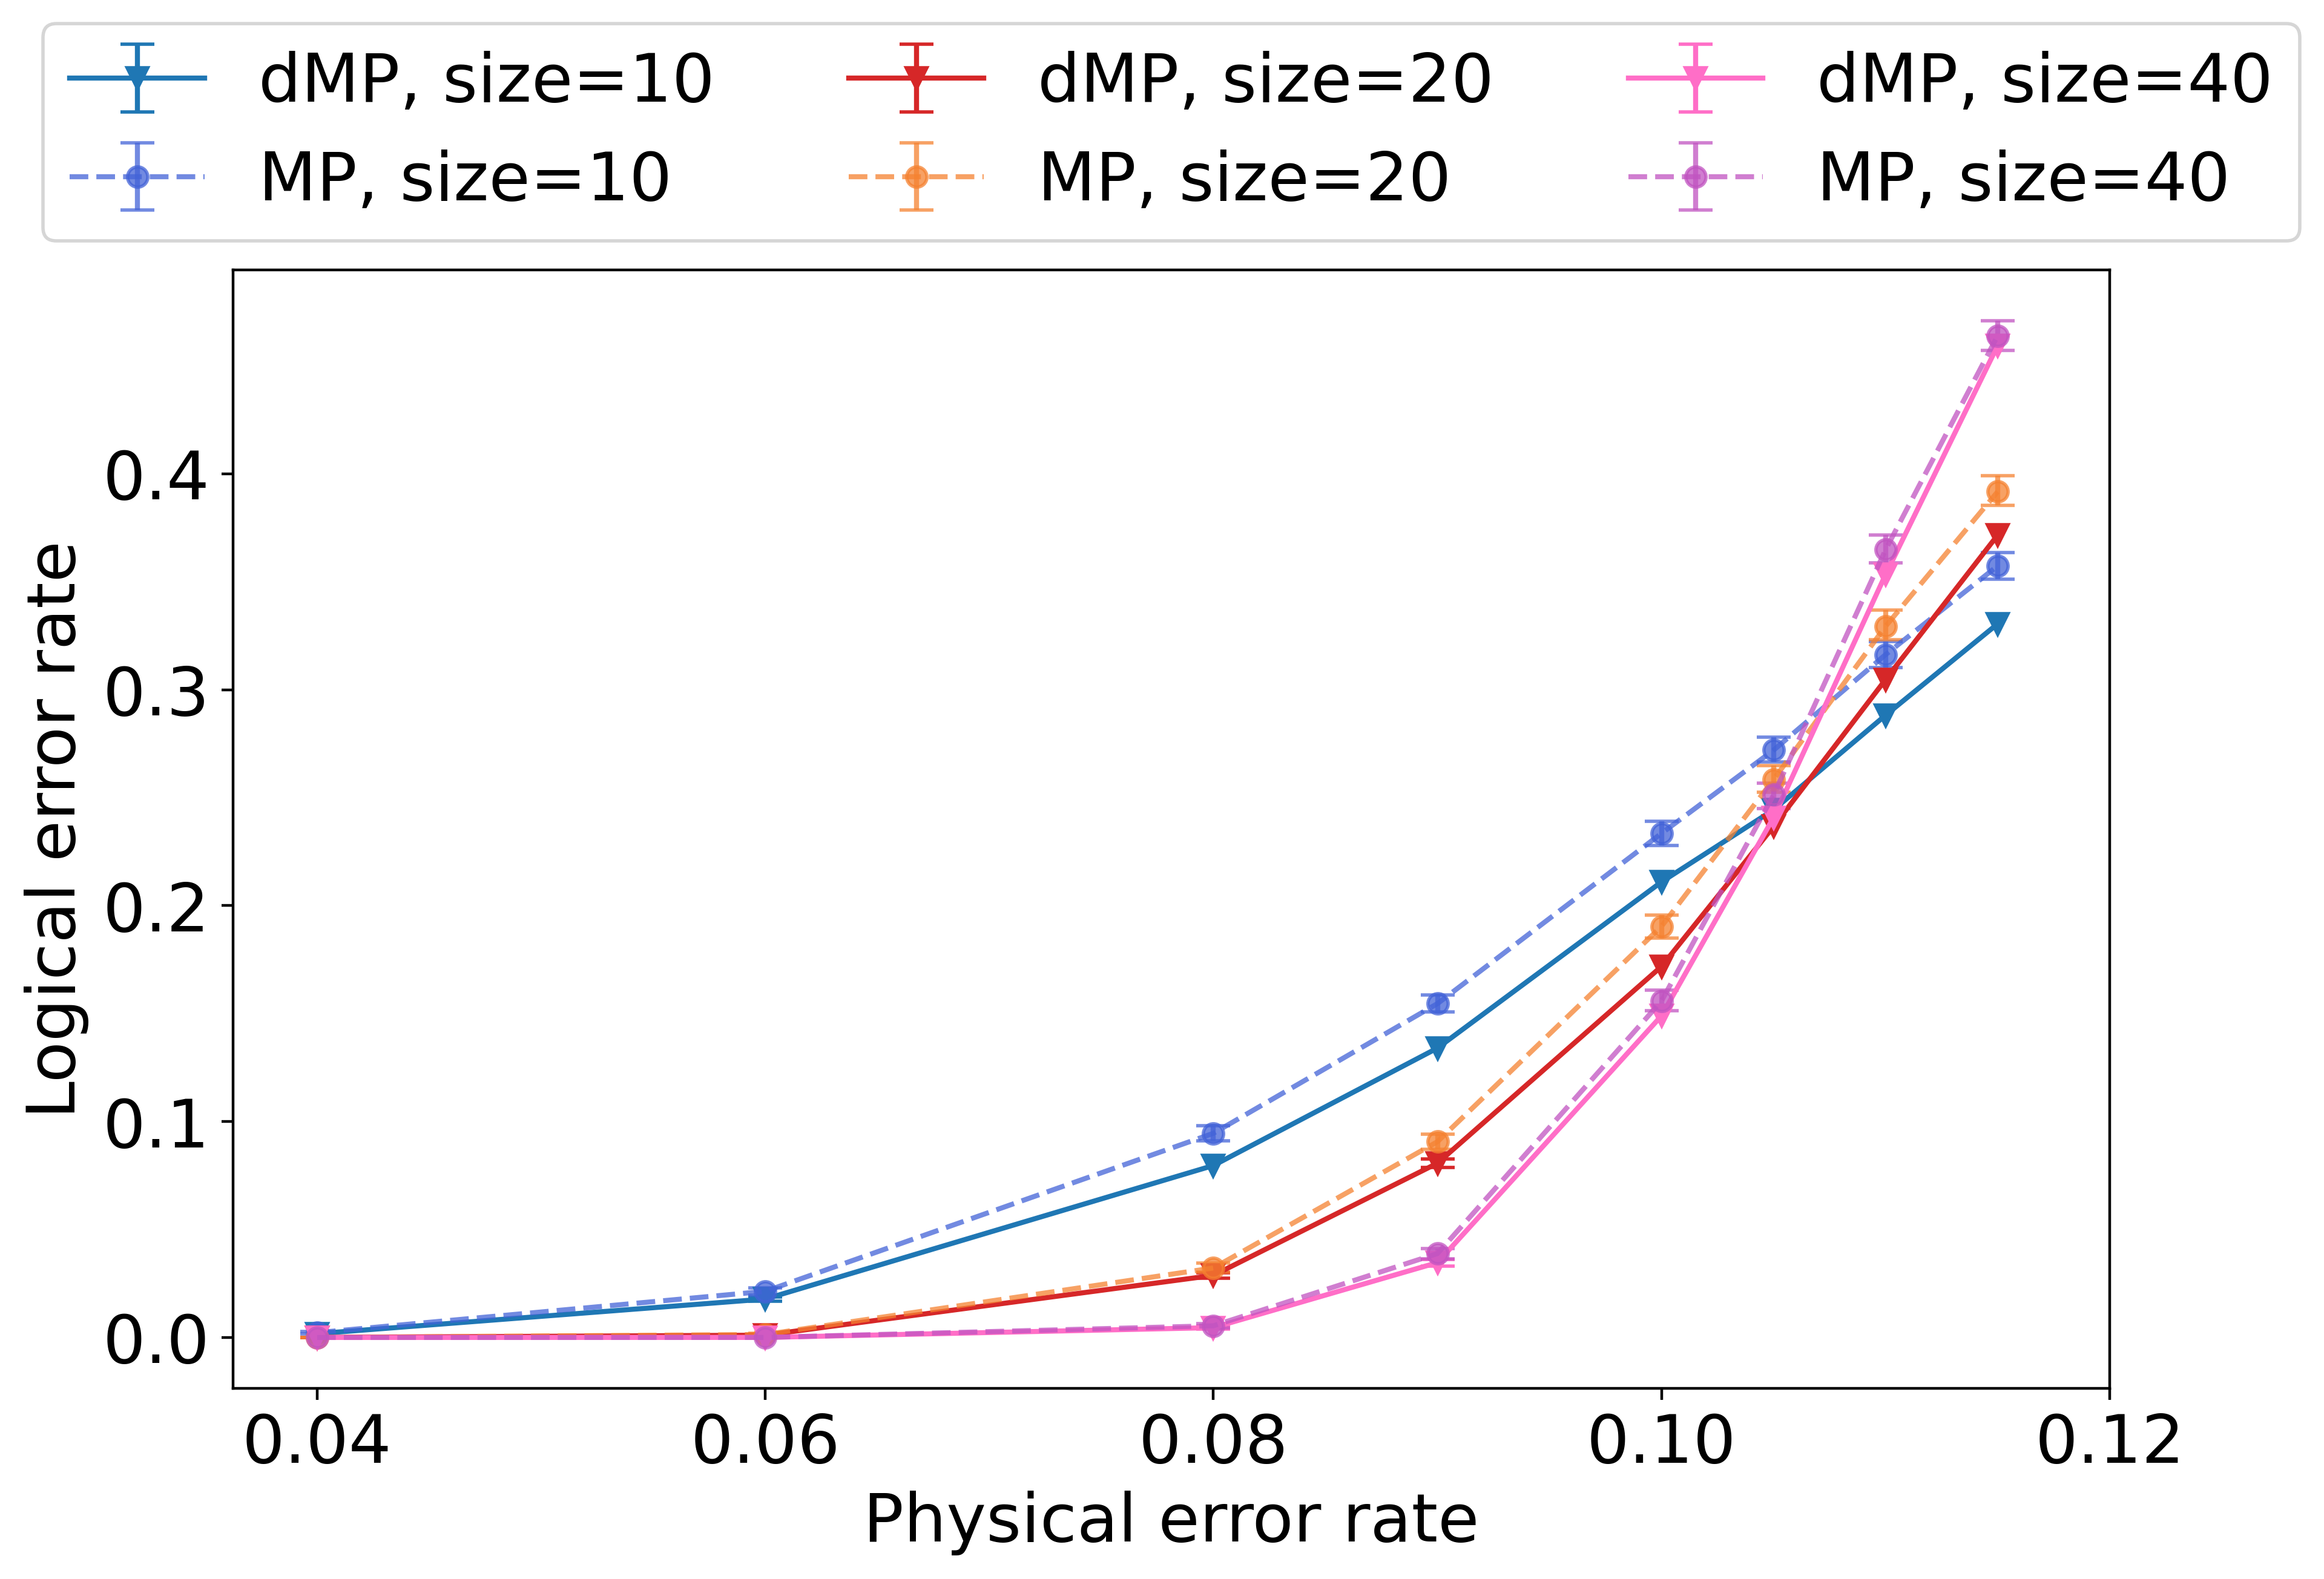
\includegraphics[width=\textwidth]{fig/dMP_vs_MP_even.png}
			% \caption{}
		\end{minipage} \hfill
		\pause
		\begin{minipage}{0.45\textwidth}
			\centering
			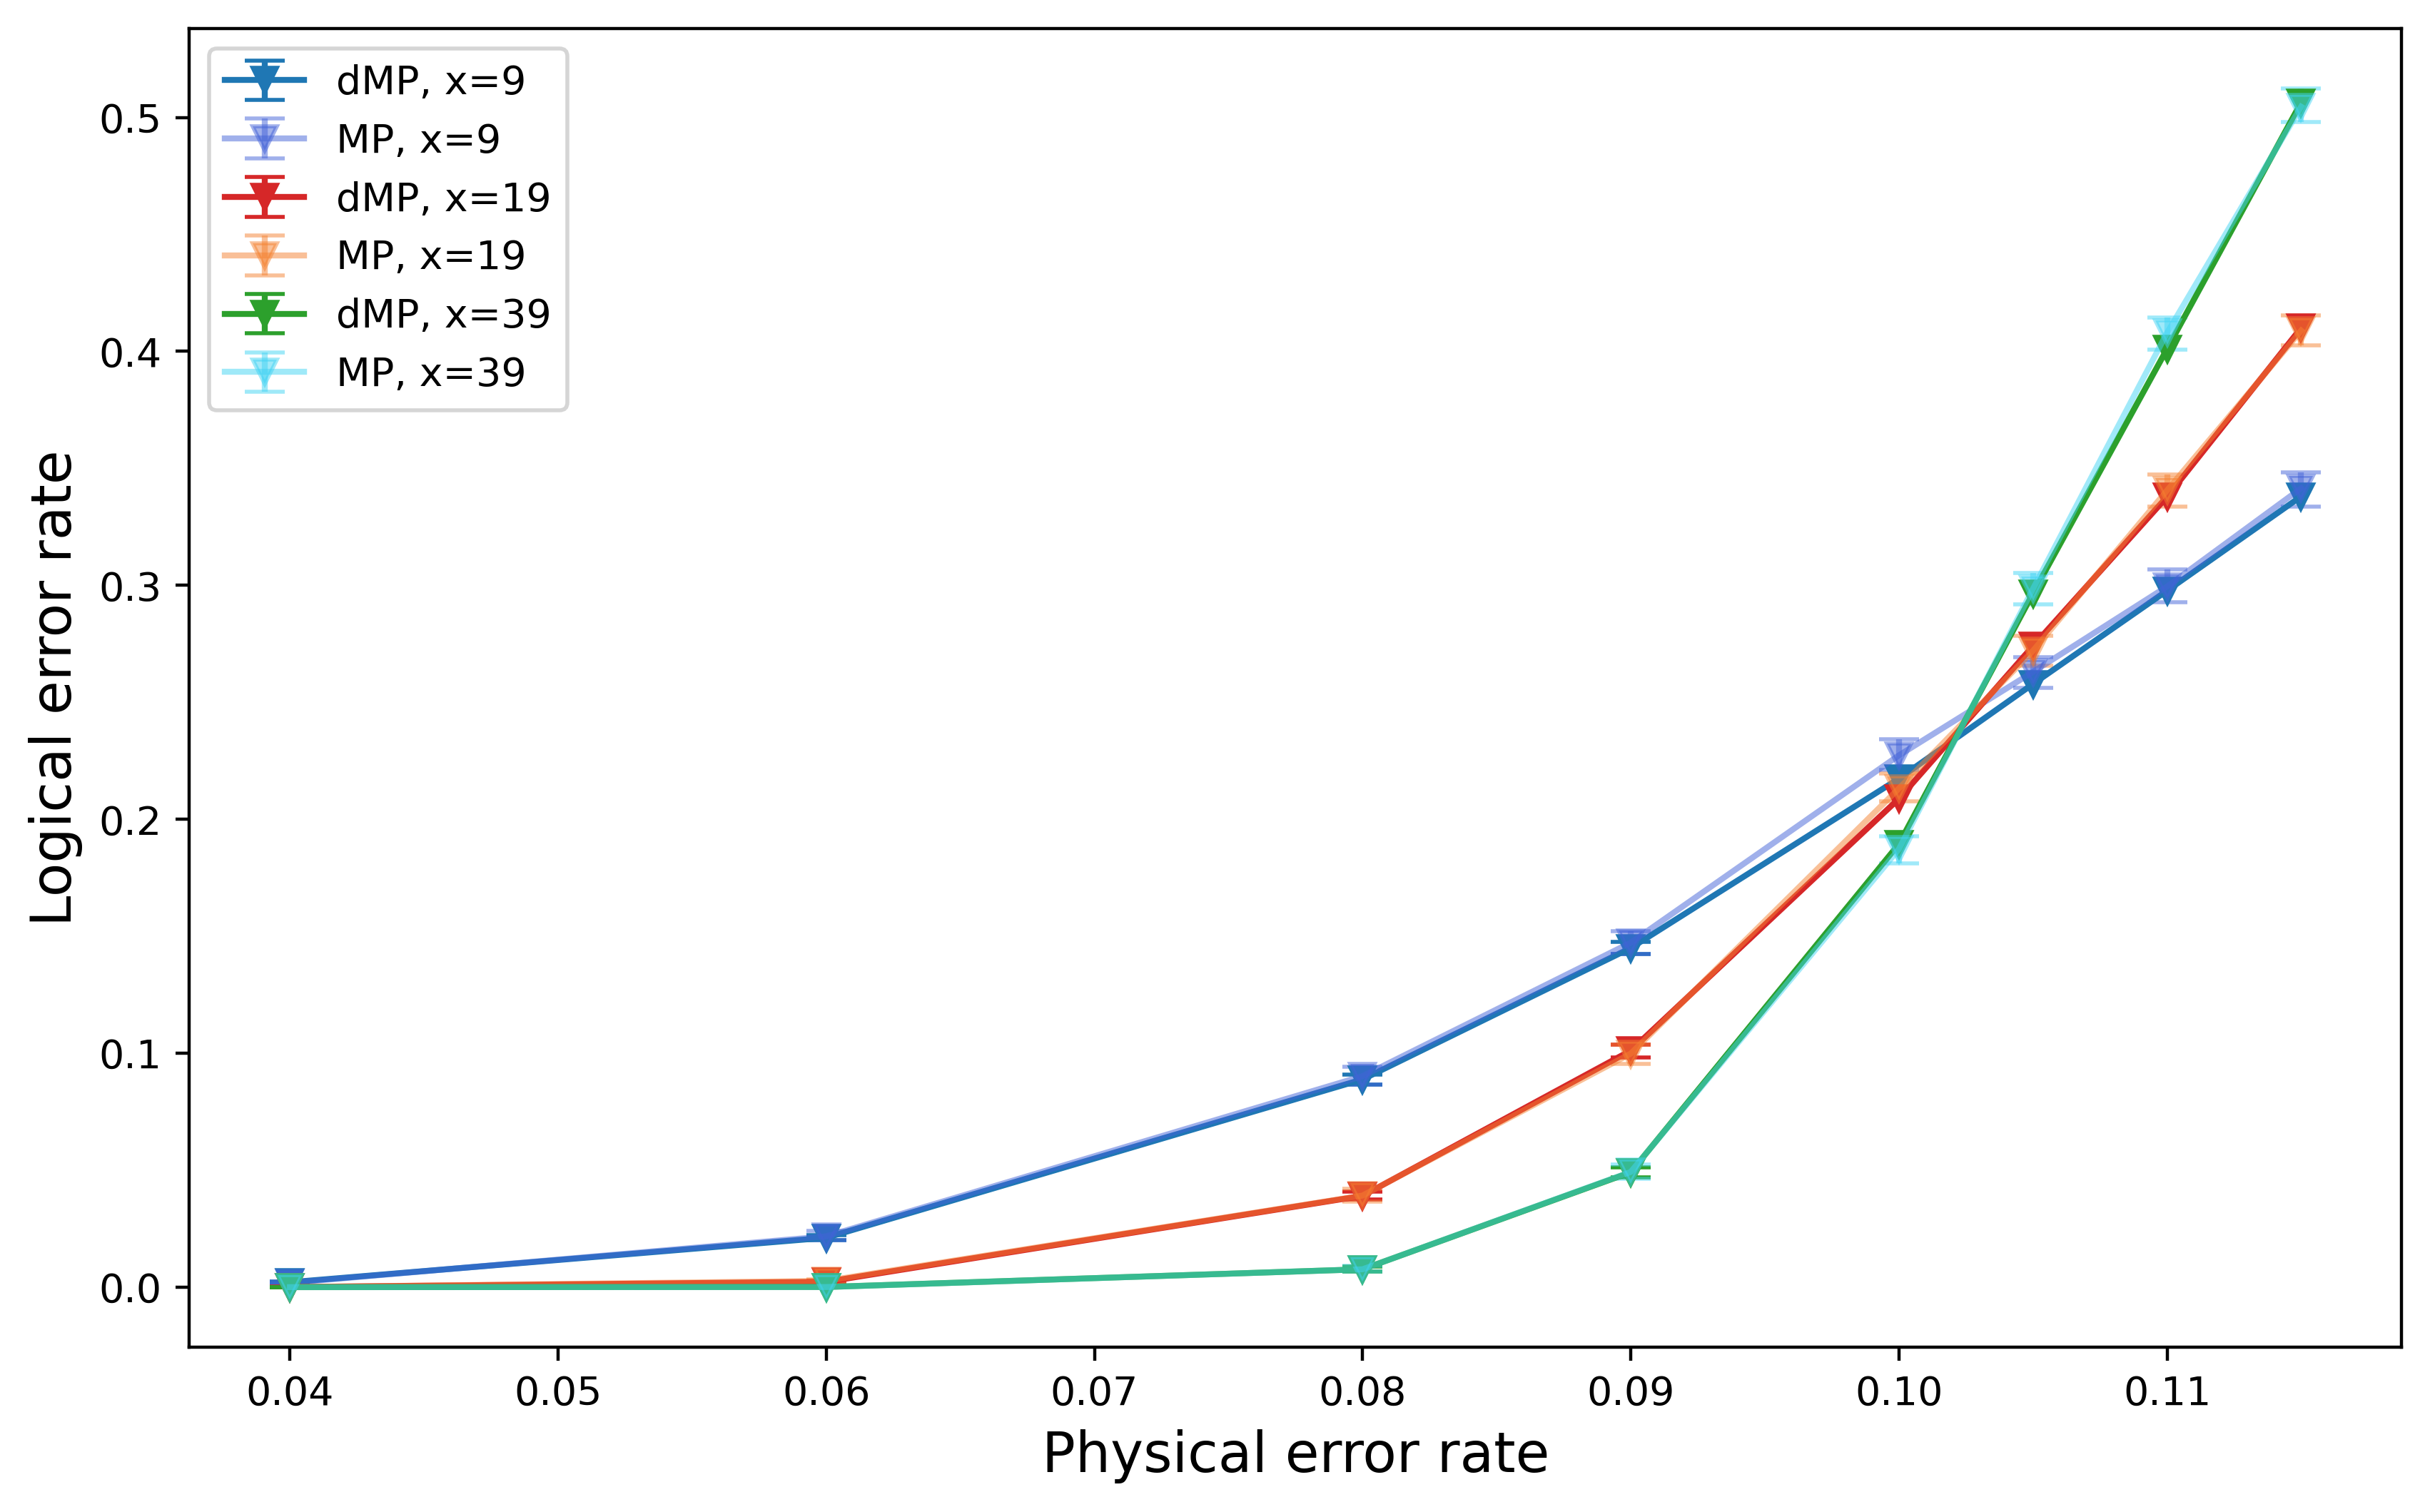
\includegraphics[width=\textwidth]{fig/dMP_vs_MP_odd.png}
			% \caption{}
		\end{minipage}
	\end{figure}
\end{frame}


\begin{frame}{Results - Intuition for dMP}
    % First slide: Basic decoding graph
    \only<1>{
        \begin{textblock*}{6cm}(1.5cm,2.5cm)
            \begin{tikzpicture}
                \newcommand{\scaling}{0.8}
                \newcommand{\nodesize}{1}
                \newcommand{\imax}{5}
                \newcommand{\jmax}{3}

                % Draw grid lines
                \foreach \i in {0,...,\imax} {
                    \draw[gray,dotted] (\i*\scaling,-0.5*\scaling) -- (\i*\scaling,\jmax*\scaling+0.5*\scaling);
                }
                \foreach \j in {0,...,\jmax} {
                    \draw[gray,dotted] (-0.5*\scaling,\j*\scaling) -- (\imax*\scaling+0.5*\scaling,\j*\scaling);
                }

                % Draw black nodes
                \foreach \i in {0,...,\imax} {
                    \foreach \j in {0,...,\jmax} {
                        \draw (\i*\scaling, \j*\scaling) node[circle, draw, fill=black, minimum size=\nodesize mm, inner sep=0]{};
                    }
                }
            \end{tikzpicture}
        \end{textblock*}

		\begin{textblock*}{9cm}(6.5cm,3cm)
			\center
			Decoding graph of toric code at even dimension
        \end{textblock*}
    }

    % Second slide: Adds error syndromes
    \only<2-2>{
        \begin{textblock*}{6cm}(1.5cm,2.5cm)
            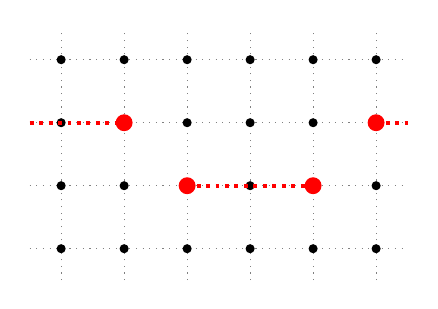
\begin{tikzpicture}
                \newcommand{\scaling}{0.8}
                \newcommand{\nodesize}{1}
                \newcommand{\imax}{5}
                \newcommand{\jmax}{3}

                % Draw grid
                \foreach \i in {0,...,\imax} {
                    \draw[gray,dotted] (\i*\scaling,-0.5*\scaling) -- (\i*\scaling,\jmax*\scaling+0.5*\scaling);
                }
                \foreach \j in {0,...,\jmax} {
                    \draw[gray,dotted] (-0.5*\scaling,\j*\scaling) -- (\imax*\scaling+0.5*\scaling,\j*\scaling);
                }

                % Draw black nodes
                \foreach \i in {0,...,\imax} {
                    \foreach \j in {0,...,\jmax} {
                        \draw (\i*\scaling, \j*\scaling) node[circle, draw, fill=black, minimum size=\nodesize mm, inner sep=0]{};
                    }
                }

                % Draw red nodes
                \foreach \i in {1,5} {
                    \foreach \j in {2} {
                        \draw (\i*\scaling, \j*\scaling) node[circle, draw, red, fill=red, minimum size=2*\nodesize mm, inner sep=0]{};
                    }
                }
                \foreach \i in {2,4} {
                    \foreach \j in {1} {
                        \draw (\i*\scaling, \j*\scaling) node[circle, draw, red, fill=red, minimum size=2*\nodesize mm, inner sep=0]{};
                    }
                }

                % Draw red dotted lines
                \draw[red, line width=0.5mm, dotted] (2*\scaling,1*\scaling) -- (4*\scaling,1*\scaling);
                \draw[red, line width=0.5mm, dotted] (-0.5*\scaling,2*\scaling) -- (1*\scaling,2*\scaling);
                \draw[red, line width=0.5mm, dotted] (5*\scaling,2*\scaling) -- (5.5*\scaling,2*\scaling);
            \end{tikzpicture}
        \end{textblock*}
		\begin{textblock*}{9cm}(7cm,3cm)
			\begin{itemize}
				\item Minimum weight error compatible with partial error information
				\item Can not be deformed without changing weight
			\end{itemize}
        \end{textblock*}
    }

    % Third slide: Adds error chains
    \only<3->{
		\begin{textblock*}{6cm}(1.5cm,2.5cm)
            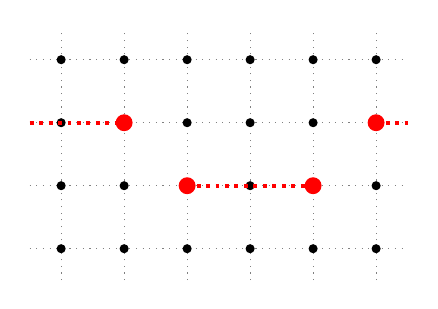
\begin{tikzpicture}
                \newcommand{\scaling}{0.8}
                \newcommand{\nodesize}{1}
                \newcommand{\imax}{5}
                \newcommand{\jmax}{3}

                % Draw grid
                \foreach \i in {0,...,\imax} {
                    \draw[gray,dotted] (\i*\scaling,-0.5*\scaling) -- (\i*\scaling,\jmax*\scaling+0.5*\scaling);
                }
                \foreach \j in {0,...,\jmax} {
                    \draw[gray,dotted] (-0.5*\scaling,\j*\scaling) -- (\imax*\scaling+0.5*\scaling,\j*\scaling);
                }

                % Draw black nodes
                \foreach \i in {0,...,\imax} {
                    \foreach \j in {0,...,\jmax} {
                        \draw (\i*\scaling, \j*\scaling) node[circle, draw, fill=black, minimum size=\nodesize mm, inner sep=0]{};
                    }
                }

                % Draw red nodes
                \foreach \i in {1,5} {
                    \foreach \j in {2} {
                        \draw (\i*\scaling, \j*\scaling) node[circle, draw, red, fill=red, minimum size=2*\nodesize mm, inner sep=0]{};
                    }
                }
                \foreach \i in {2,4} {
                    \foreach \j in {1} {
                        \draw (\i*\scaling, \j*\scaling) node[circle, draw, red, fill=red, minimum size=2*\nodesize mm, inner sep=0]{};
                    }
                }

                % Draw red dotted lines
                \draw[red, line width=0.5mm, dotted] (2*\scaling,1*\scaling) -- (4*\scaling,1*\scaling);
                \draw[red, line width=0.5mm, dotted] (-0.5*\scaling,2*\scaling) -- (1*\scaling,2*\scaling);
                \draw[red, line width=0.5mm, dotted] (5*\scaling,2*\scaling) -- (5.5*\scaling,2*\scaling);
            \end{tikzpicture}
        \end{textblock*}
        \begin{textblock*}{6cm}(8.5cm,2.5cm)
            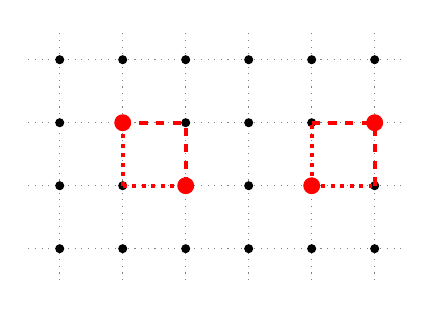
\begin{tikzpicture}
                \newcommand{\scaling}{0.8}
                \newcommand{\nodesize}{1}
                \newcommand{\imax}{5}
                \newcommand{\jmax}{3}

                % Draw grid
                \foreach \i in {0,...,\imax} {
                    \draw[gray,dotted] (\i*\scaling,-0.5*\scaling) -- (\i*\scaling,\jmax*\scaling+0.5*\scaling);
                }
                \foreach \j in {0,...,\jmax} {
                    \draw[gray,dotted] (-0.5*\scaling,\j*\scaling) -- (\imax*\scaling+0.5*\scaling,\j*\scaling);
                }

                % Draw black nodes
                \foreach \i in {0,...,\imax} {
                    \foreach \j in {0,...,\jmax} {
                        \draw (\i*\scaling, \j*\scaling) node[circle, draw, fill=black, minimum size=\nodesize mm, inner sep=0]{};
                    }
                }

                % Draw red nodes
                \foreach \i in {1,5} {
                    \foreach \j in {2} {
                        \draw (\i*\scaling, \j*\scaling) node[circle, draw, red, fill=red, minimum size=2*\nodesize mm, inner sep=0]{};
                    }
                }
                \foreach \i in {2,4} {
                    \foreach \j in {1} {
                        \draw (\i*\scaling, \j*\scaling) node[circle, draw, red, fill=red, minimum size=2*\nodesize mm, inner sep=0]{};
                    }
                }

                % Draw error chains
                \draw[red, line width=0.5mm, dotted] (1*\scaling,1*\scaling) -- (2*\scaling,1*\scaling);
                \draw[red, line width=0.5mm, dotted] (1*\scaling,1*\scaling) -- (1*\scaling,2*\scaling);
                \draw[red, line width=0.5mm, dashed] (1*\scaling,2*\scaling) -- (2*\scaling,2*\scaling);
                \draw[red, line width=0.5mm, dashed] (2*\scaling,1*\scaling) -- (2*\scaling,2*\scaling);

                \draw[red, line width=0.5mm, dotted] (4*\scaling,1*\scaling) -- (5*\scaling,1*\scaling);
                \draw[red, line width=0.5mm, dotted] (4*\scaling,1*\scaling) -- (4*\scaling,2*\scaling);
                \draw[red, line width=0.5mm, dashed] (4*\scaling,2*\scaling) -- (5*\scaling,2*\scaling);
                \draw[red, line width=0.5mm, dashed] (5*\scaling,1*\scaling) -- (5*\scaling,2*\scaling);
            \end{tikzpicture}
        \end{textblock*}
    }
\end{frame}

\begin{frame}{Results - Enhanced Pymatching}
	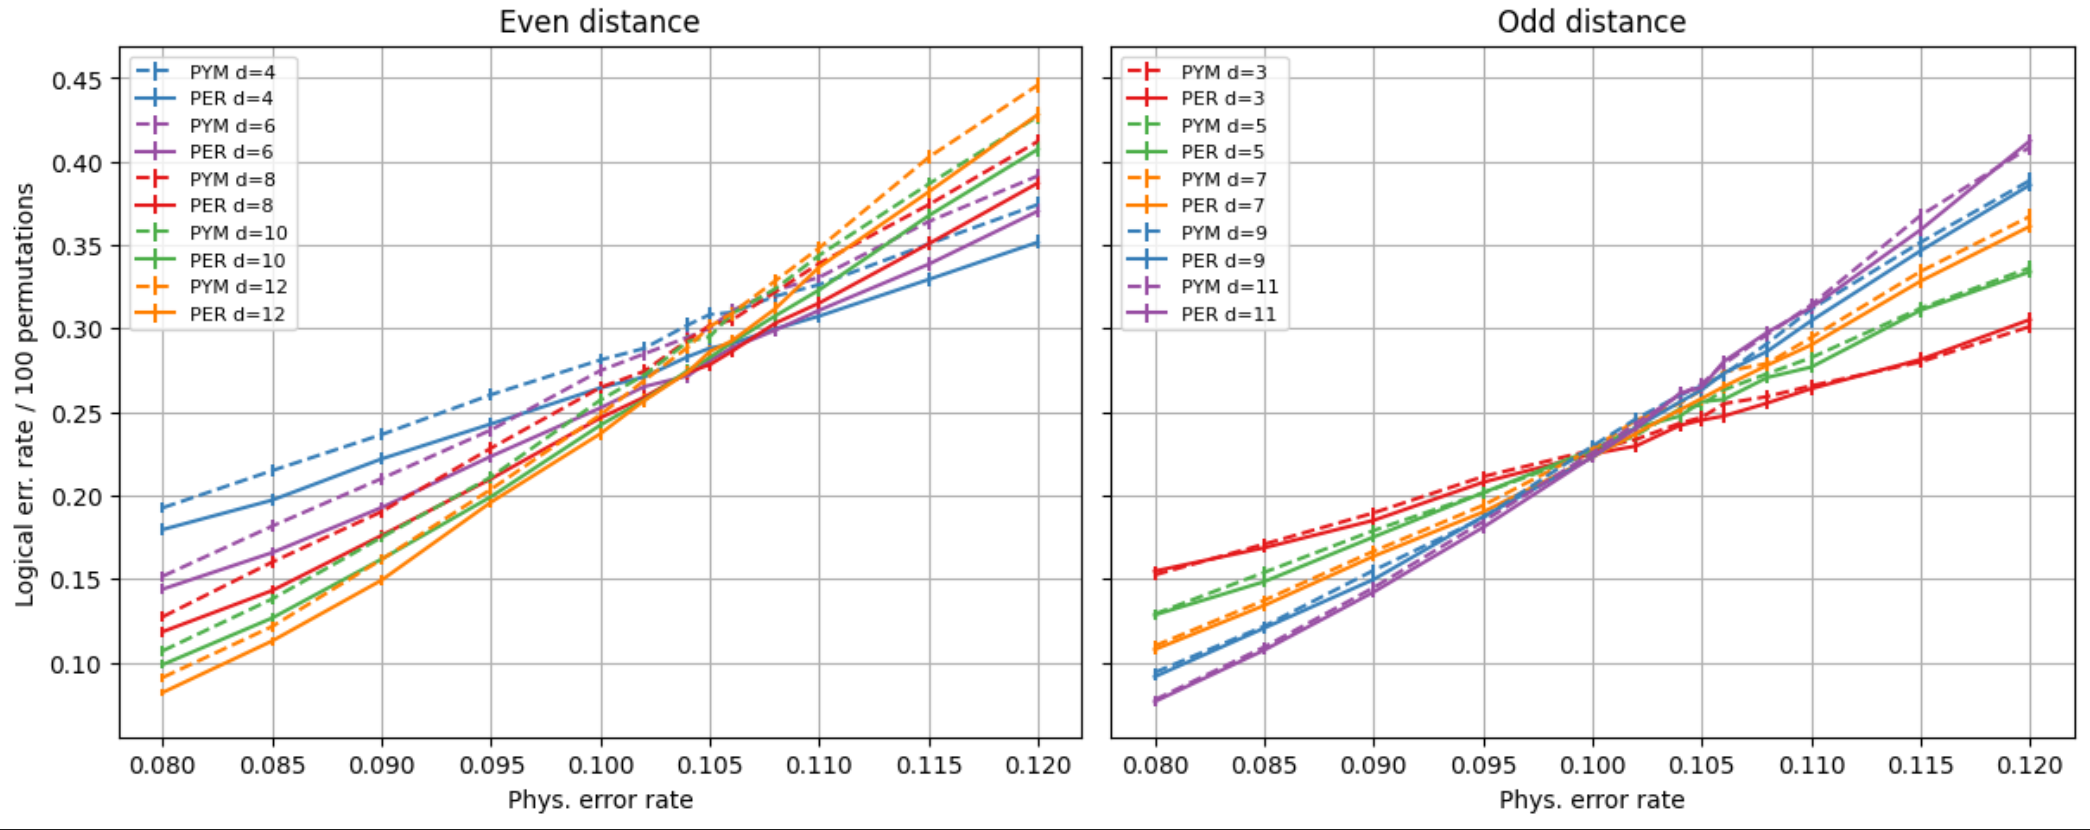
\includegraphics[width=\textwidth]{fig/provisional_pymatching.png}
	% \begin{figure}[h!]
	% 	\centering
	% 	\begin{minipage}{0.45\textwidth}
	% 		\centering
	% 		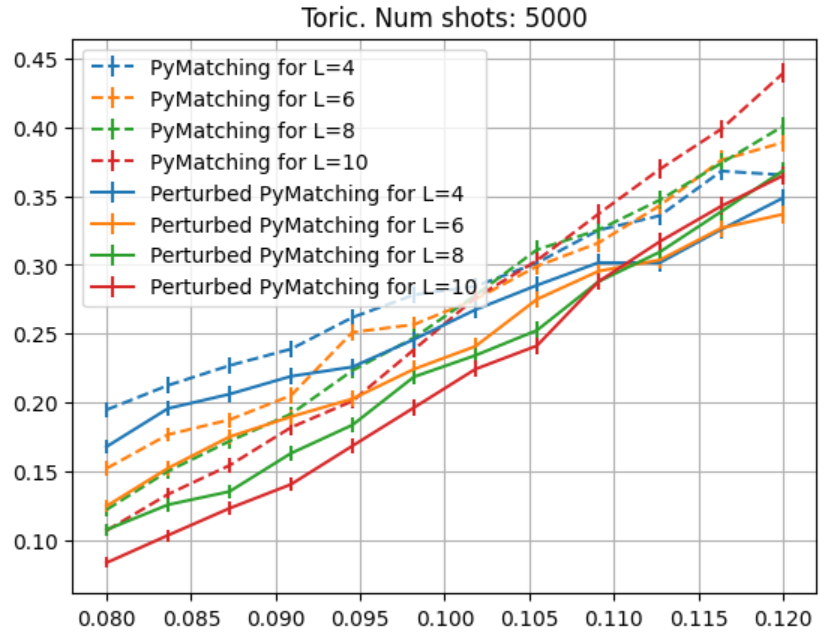
\includegraphics[width=\textwidth]{fig/PymatchingToric2.png}
	% 	\end{minipage} \hfill
	% 	\begin{minipage}{0.45\textwidth}
	% 		\centering
	% 		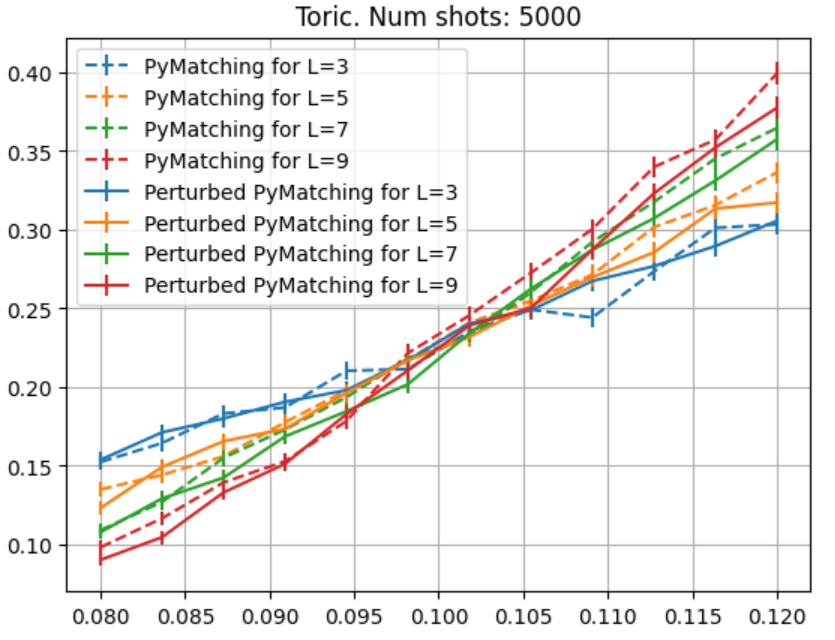
\includegraphics[width=\textwidth]{fig/PymatchingToric1.png}
	% 	\end{minipage}
	% \end{figure}
\end{frame}

\begin{frame}{Preliminary Results - Gaussian Noise}
	\centering
	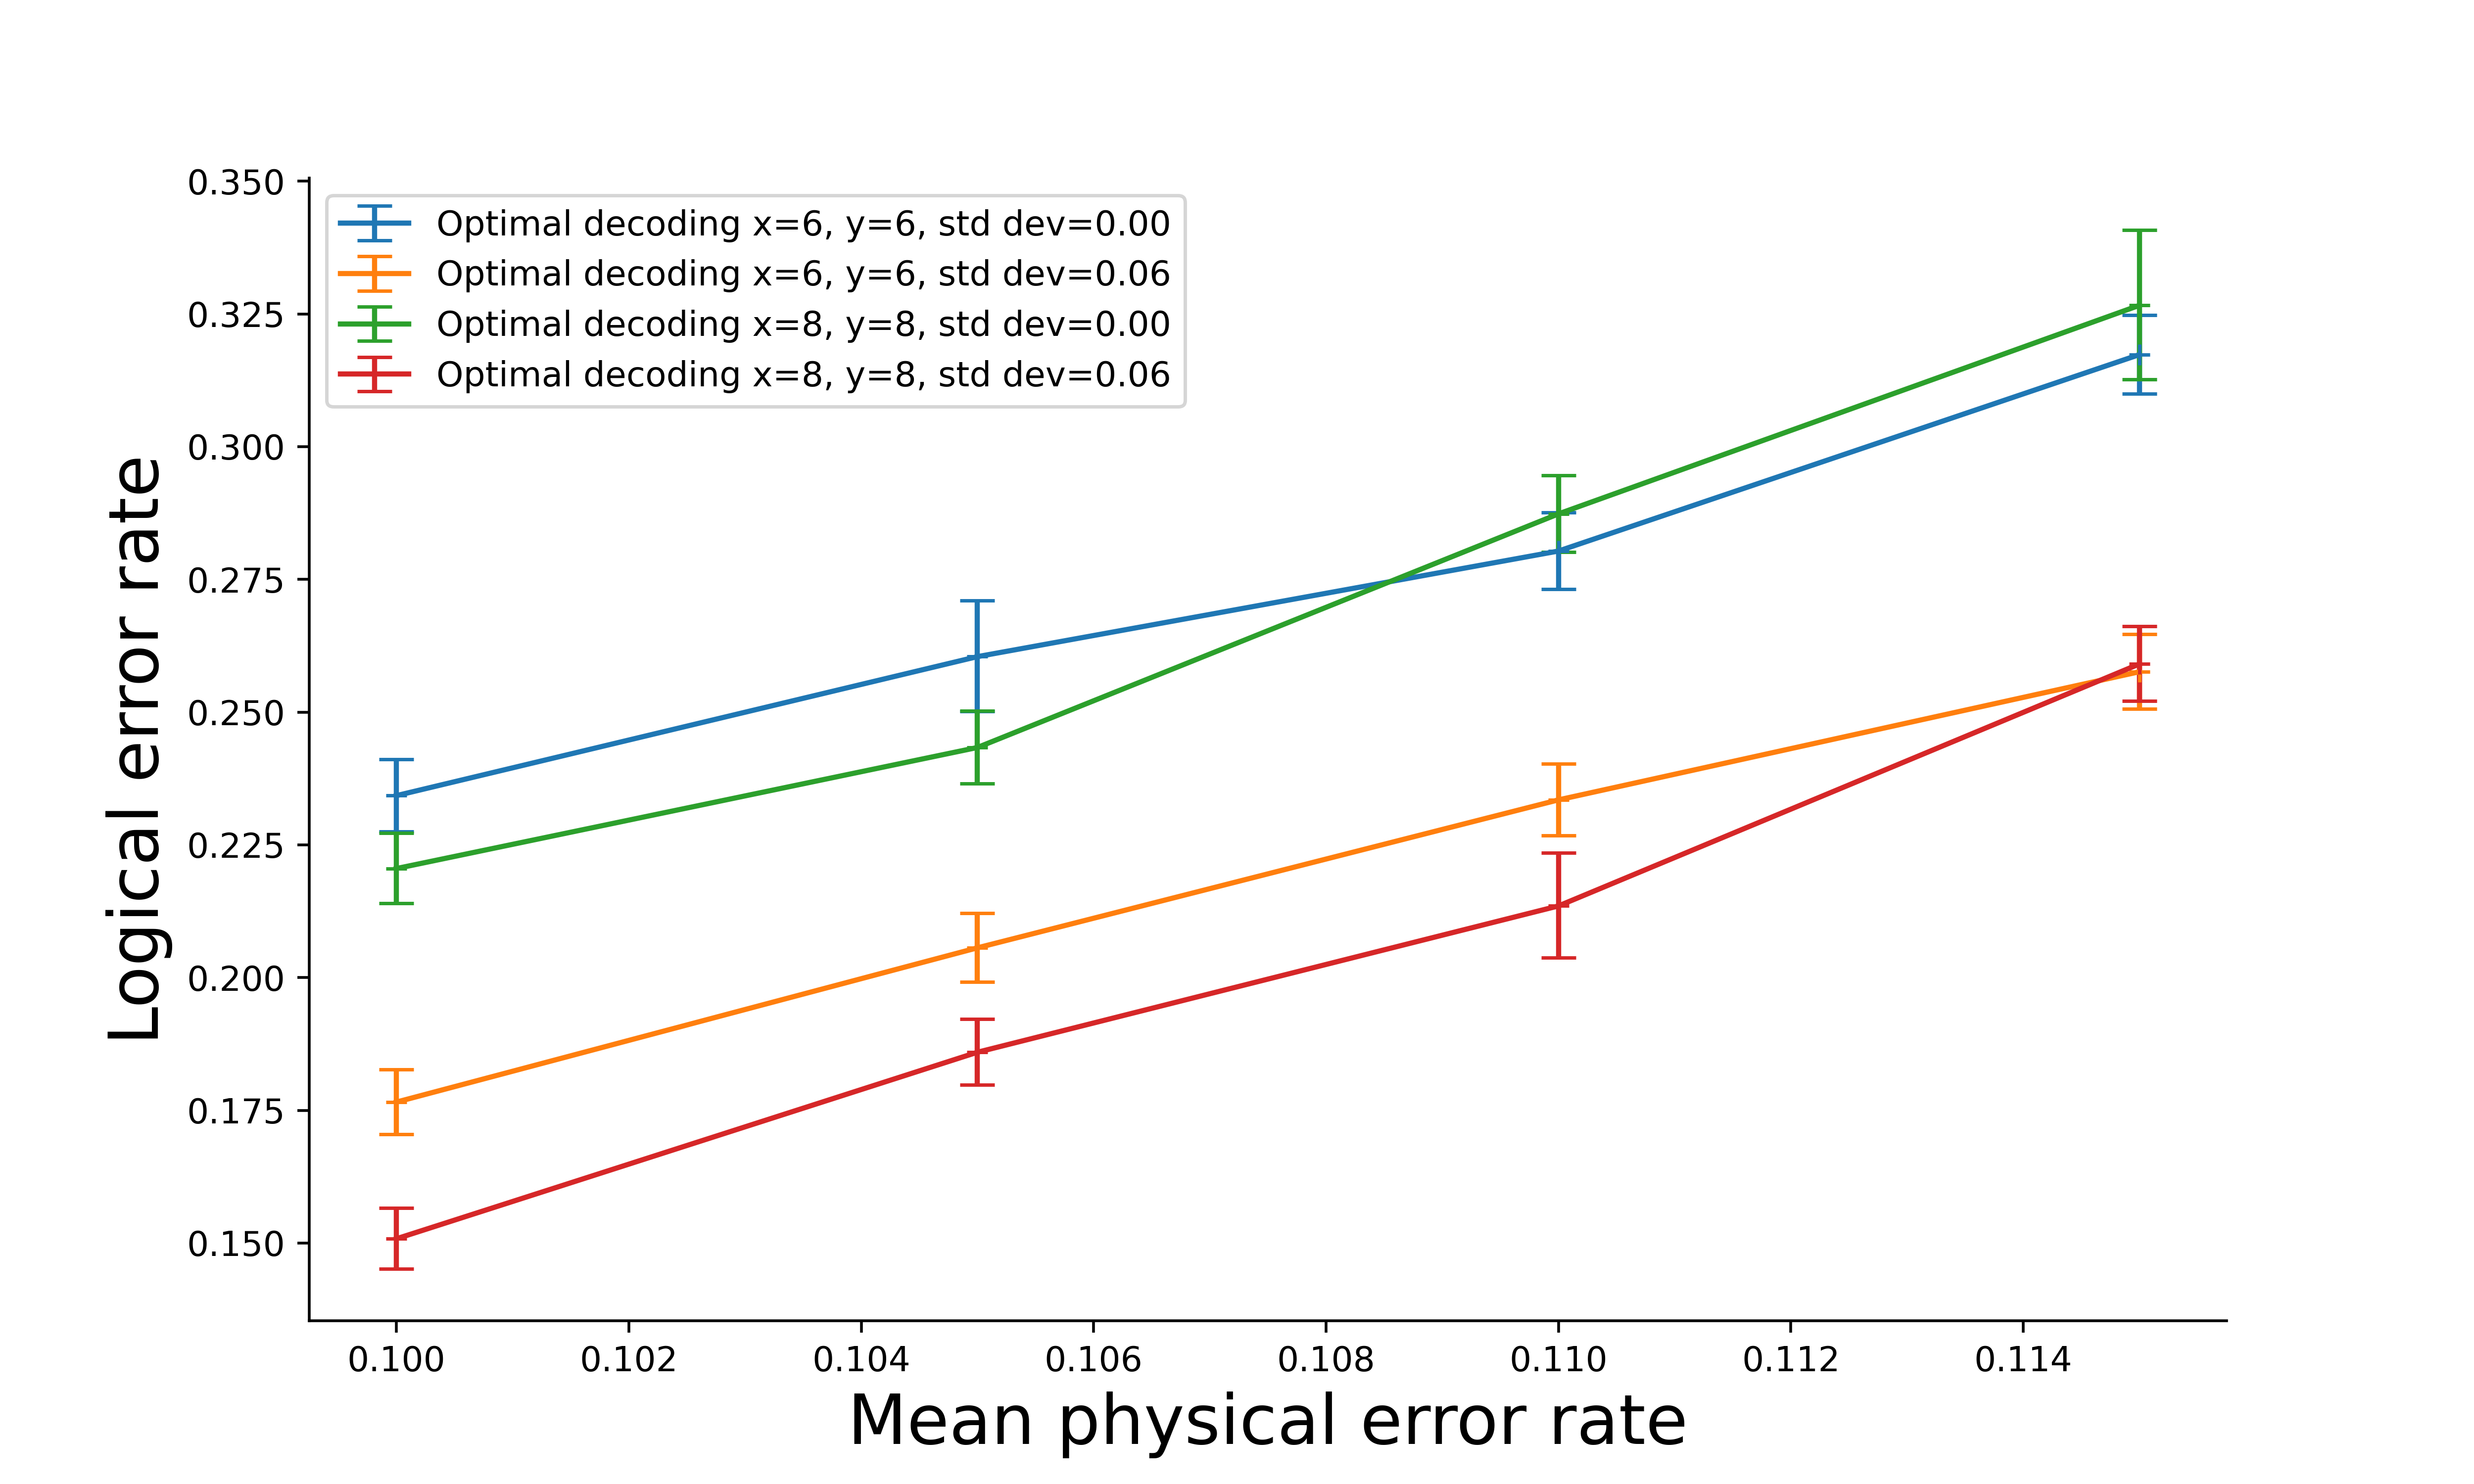
\includegraphics[width=0.7\textwidth]{fig/Optimal_decoding_varying_stddev.png}
\end{frame}

\begin{frame}{Research plan}
	\begin{table}[h]
        \renewcommand{\arraystretch}{1.5} % Increase row spacing
        \small
		\begin{tabular}{c|p{10cm}}
			\textbf{Time} &  \textbf{Objective} \\
			\hline
			February 2025 & Presented framework at QIP 2025 by poster \\
			April-May 2025 & Submit paper on optimization opportunities of MWPM by degeneracy of ground states \\
			2025 & Incoroporate TN approximate ML decoder into framework $\&$ investigate further alternatives \\
			2025 & Incorporate more realistic noise model into framework $\&$ investigate its influence \\
			2025-2026 & Potentially QuaSA: Implementation of error correcting codes, deduction of noise model and simulation of hardware\\
		\end{tabular}
	\end{table}
\end{frame}

\begin{frame}{Work plan}
	\begin{table}[h]
		\fontsize{8pt}{9pt}\selectfont
		\center
		{\renewcommand{\arraystretch}{2}
		\begin{tabular}{l@{\hspace{1em}}p{4.5cm}p{3cm}l@{\hspace{1em}}p{1.7cm}}
            \toprule
            Authorship & Title & Type  & Year & Status   \\
            \midrule
            1st-author & Estimating ML and MP decoder performance in stabilizer codes, and the room for performance gains from ensembling in MP decoders & Physical Review A & 2025 & submission April-May \\
			co-author & Exploration of Design Alternatives for Reducing Idle Time in Shor's Algorithm & IEEE Transactions on Quantum Engineering & 2025 & submitted \\
            to be discussed & Extending current results to realistic noise models & Journal & 2025-26 & Future work \\
			to be discussed & QuaSA: Error dynamics of Quantum Memory & Journal & 2026 & Future work \\
            \bottomrule
        \end{tabular}
		}
	\end{table} \vfill
\end{frame}

\begin{frame}{Conclusion and Outlook}
	\begin{textblock*}{14cm}(1.5cm,2cm)
		\raisebox{-0.5cm}{
\includegraphics[width=0.15\textwidth]{fig/Noise.png}}
		\begin{tikzpicture}[overlay]
			\draw[->, line width=0.8mm, black] (0.5, 0.1) -- (4,0.1);
			\draw[-, line width=0.8mm, black] (0.5, 0.3) -- (0.5,-0.1);
		\end{tikzpicture}
		\hspace{4.5cm}
		Optimal code performance estimate
	\end{textblock*}
	\vspace{3cm}
	\small
	\begin{itemize}
		\item \textbf{Framework:} Applicable to all stabilizer codes under Pauli noise
		\item \textbf{Optimal decoding:} Developed efficient estimator of success rate
		\item \textbf{Decoder Optimization:} Improved MWPM by degeneracy of ground states
		\item \textbf{Near future:} Investigate noise influence on optimal performance
		\item \textbf{Further:} Incorporate realistic noise model which requires new methods like TN
	\end{itemize}
\end{frame}

\begin{frame}
	\begin{center}
		{\huge\textbf{Thank you for your attention!}}
	\end{center}
\end{frame}

\printbibliography

\end{document}




% \begin{frame}{Suboptimal Decoders for Surface Codes}
% 	\only<1-1>{
% 		\textbf{\hspace{1cm}Minimum Weight Perfect Matching~\citeauthoryear{edmonds_paths_1965}}
% 	}
% 	\only<2-2>{
% 		\textbf{\hspace{1cm}Minimum Weight Perfect Matching~\citeauthoryear{edmonds_paths_1965}}
% 		\begin{itemize}
% 			\item Speed improved: Sparse blossom $O(n^{1.32})$~\citeauthoryear{higgott_sparse_2025}, fusion blossom $O(n)$~\citeauthoryear{wu_fusion_2023}
% 			\item Sparse blossom: Real time decoding $0.1\%$ depolarising noise on distance-17 surface code \citeauthoryear{higgott_sparse_2025}
% 		\end{itemize}
% 	}
% 	\only<3-3>{
% 		\textbf{\hspace{1cm}Minimum Weight Perfect Matching~\citeauthoryear{edmonds_paths_1965}}
% 		\begin{itemize}
% 			\item Speed improved: Sparse blossom $O(n^{1.32})$~\citeauthoryear{higgott_sparse_2025}, fusion blossom $O(n)$~\citeauthoryear{wu_fusion_2023}
% 			\item Sparse blossom: Real time decoding $0.1\%$ depolarising noise on distance-17 surface code \citeauthoryear{higgott_sparse_2025}
% 			\item Improved performance: Ensembling~\citeauthoryear{shutty_efficient_2024, jones_improved_2024}
% 			\item Noise aware: Weights calibrated by noise~\citeauthoryear{iolius_performance_2022, hockings_improving_2025}, correlated MWPM~\citeauthoryear{fowler_optimal_2013}
% 		\end{itemize}
% 		% \cite{fowler_towards_2012}
% 	}
% 	\only<4->{
% 		\textbf{\hspace{1cm}Tensor Network Decoder~\citeauthoryear{bravyi_efficient_2014}}
% 		\begin{itemize}
% 			\item Surface Code $\rightarrow$ Tensor Network
% 			\item Optimal decoding $\rightarrow$ TN contraction
% 			\item Approximate contraction $\rightarrow$ approximate optimal decoding
% 			\item Generalised to arbitrary 2D codes \citeauthoryear{chubb_general_2021}
% 			\item Noise aware~\citeauthoryear{darmawan_optimal_2024}
% 		\end{itemize}
% 	}
% \end{frame}

% \begin{frame}{Optimal Code Capacity Thresholds}
% 	Quality marker: $p_{\text{threshold}}$
% 	\begin{table}[h]
%         \renewcommand{\arraystretch}{1.5} % Increase row spacing
%         \small
% 		\begin{tabular}{c|c|p{6cm}}
% 			\textbf{Code} & \textbf{Noise} & \textbf{Publications} \\
% 			\hline
% 			Toric Code & Independent X, Z errors & \citeauthoryear{merz_two-dimensional_2001, honecker_nishimori_2001} \\
% 			 & Depolarizing Noise & \citeauthoryear{bombin_strong_2012} \\
% 			 & Correlated Noise & \citeauthoryear{chubb_statistical_2019}\\
% 			\hline
% 			Surface Code & Independent X, Z errors & \citeauthoryear{bravyi_efficient_2014} \\
% 			& Depolarizing Noise & \citeauthoryear{bravyi_efficient_2014} \\
% 			& Amplitude Damping & \citeauthoryear{darmawan_tensor-network_2017} \\
% 			& Coherent Noise & \citeauthoryear{behrends_statistical_2024, bao_phases_2024}
% 		\end{tabular}
% 		\textcolor{red}{Optimal curves for toric code}
% 	\end{table}
% \end{frame}

% \begin{frame}{Surface Code Suboptimal Decoders}
% 	\begin{textblock*}{9cm}(7cm,2.5cm)
%         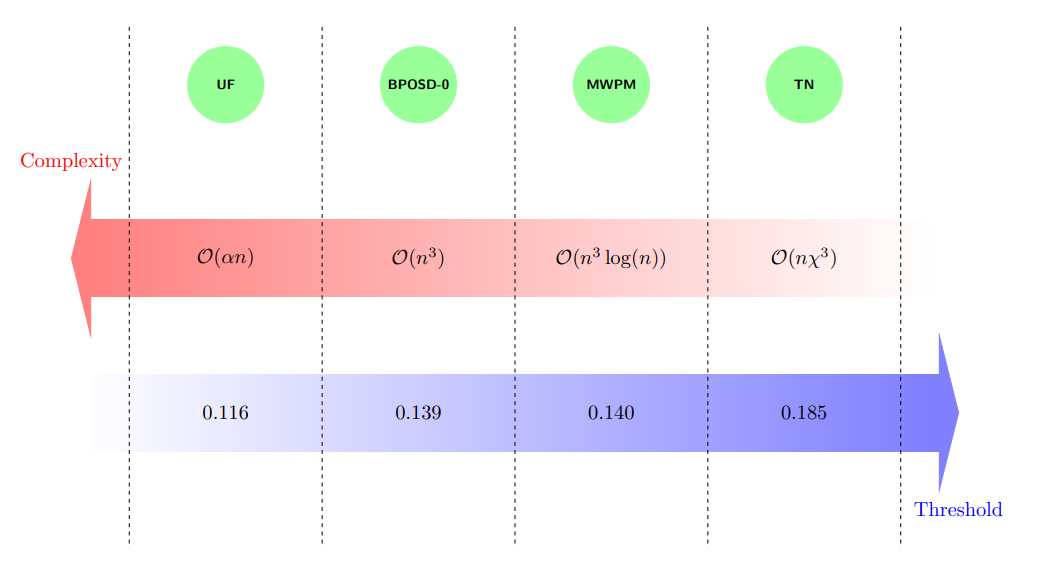
\includegraphics[width=1\textwidth]{fig/Screenshot from 2025-03-24 15-21-55.png}
%     \end{textblock*}
% 	\begin{textblock*}{2cm}(12.5cm,3.4cm)
% 		\begin{tiny}
% 			\cite{edmonds_paths_1965}
% 		\end{tiny}
% 	\end{textblock*}
% 	\begin{textblock*}{2cm}(9.2cm,3.4cm)
% 		\begin{tiny}
% 			\cite{delfosse_almost-linear_2021}
% 		\end{tiny}
% 	\end{textblock*}
% 	\begin{textblock*}{2cm}(10.8cm,3.4cm)
% 		\begin{tiny}
% 			\cite{panteleev_degenerate_2021}
% 		\end{tiny}
% 	\end{textblock*}
% 	\begin{textblock*}{2cm}(14.1cm,3.4cm)
% 		\begin{tiny}
% 			\cite{bravyi_efficient_2014,chubb_general_2021}
% 		\end{tiny}
% 	\end{textblock*}

% 	\only<1-1>{
% 		\begin{textblock*}{3.5cm}(1cm,4cm)
% 			\begin{tcolorbox}[colback=osakared!5!white, colframe=osakared, width=4cm, arc=2mm]
% 				\center
% 				Backlog problem
% 			\end{tcolorbox}
% 		\end{textblock*}
% 	}
% 	% \pause
% 	% \only<2-2>{
% 	% \begin{textblock*}{5.8cm}(0.1cm,3.5cm)
% 	% 	\begin{small}
% 	% 	\textbf{Union Find}
% 	% 	\begin{itemize}
% 	% 		\item Pauli errors $\rightarrow$ erasure errors
% 	% 		\item almost linear time complexity
% 	% 		\item Noise aware \cite{higgott_improved_2023}
% 	% 	\end{itemize}
% 	% 	\end{small}
% 	% \end{textblock*}
% 	% }
% 	% \pause
% 	% \only<3-3>{
% 	% \begin{textblock*}{5.8cm}(0.1cm,3cm)
% 	% 	\begin{small}
% 	% 	\textbf{Belief Propagation}
% 	% 	\begin{itemize}
% 	% 		\item Acts on general Tanner graphs $\rightarrow$ any QLDPC decoder
% 	% 		\item Issues with highly degenerate codes (split-belief phenomenon) \cite{poulin_iterative_2008, roffe_decoding_2020}
% 	% 		\item Ordered statistics decoding (BP+OSD) to enhance performance \cite{panteleev_degenerate_2021}
% 	% 	\end{itemize}
% 	% 	\end{small}
% 	% \end{textblock*}
% 	% }
% 	\pause
% 	\only<2-2>{
% 	\begin{textblock*}{7cm}(0cm,2cm)
% 		\begin{small}
% 			\textbf{\hspace{1cm}Minimum Weight Perfect Matching}
% 			\begin{itemize}
% 				\item Complexity improved: Sparse blossom $O(n^{1.32})$, fusion blossom $O(n)$
% 				\item Sparse blossom: Real time decoding $0.1\%$ depolarising noise on distance-17 surface code \citeauthoryear{higgott_sparse_2025}
% 				\item Improved performance: Ensembling~\citeauthoryear{shutty_efficient_2024, jones_improved_2024}
% 				\item Noise aware: Weights calibrated by noise~\citeauthoryear{iolius_performance_2022, hockings_improving_2025}, correlated MWPM~\citeauthoryear{fowler_optimal_2013}
% 			\end{itemize}
% 		\end{small}
% 	\end{textblock*}
% 	\begin{textblock*}{10cm}(9.7cm,3.5cm)
% 		\begin{tikzpicture}
% 			\draw[->, bend right=70] (2.5cm,0cm) to node[below] {\tiny{\cite{fowler_towards_2012, wu_fusion_2023, higgott_sparse_2025}}} (0cm,0cm);
% 		\end{tikzpicture}
% 	\end{textblock*}
% 	}
% 	\pause
% 	\only<3-3>{
% 	\begin{textblock*}{7cm}(0cm,3cm)
% 		\begin{small}
% 			\textbf{\hspace{1cm}Tensor Network Decoder}
% 			\begin{itemize}
% 				\item Surface Code $\rightarrow$ Tensor Network
% 				\item Optimal decoding $\rightarrow$ TN contraction
% 				\item Approximate contraction $\rightarrow$ approximate optimal decoding
% 				\item Generalised to arbitrary 2D codes \citeauthoryear{chubb_general_2021}
% 				\item Noise aware~\citeauthoryear{darmawan_optimal_2024}
% 			\end{itemize}
% 		\end{small}
% 	\end{textblock*}
% 	}
% \end{frame}


% \begin{frame}{Tackling Quantum Errors}
% 	\begin{center}
%         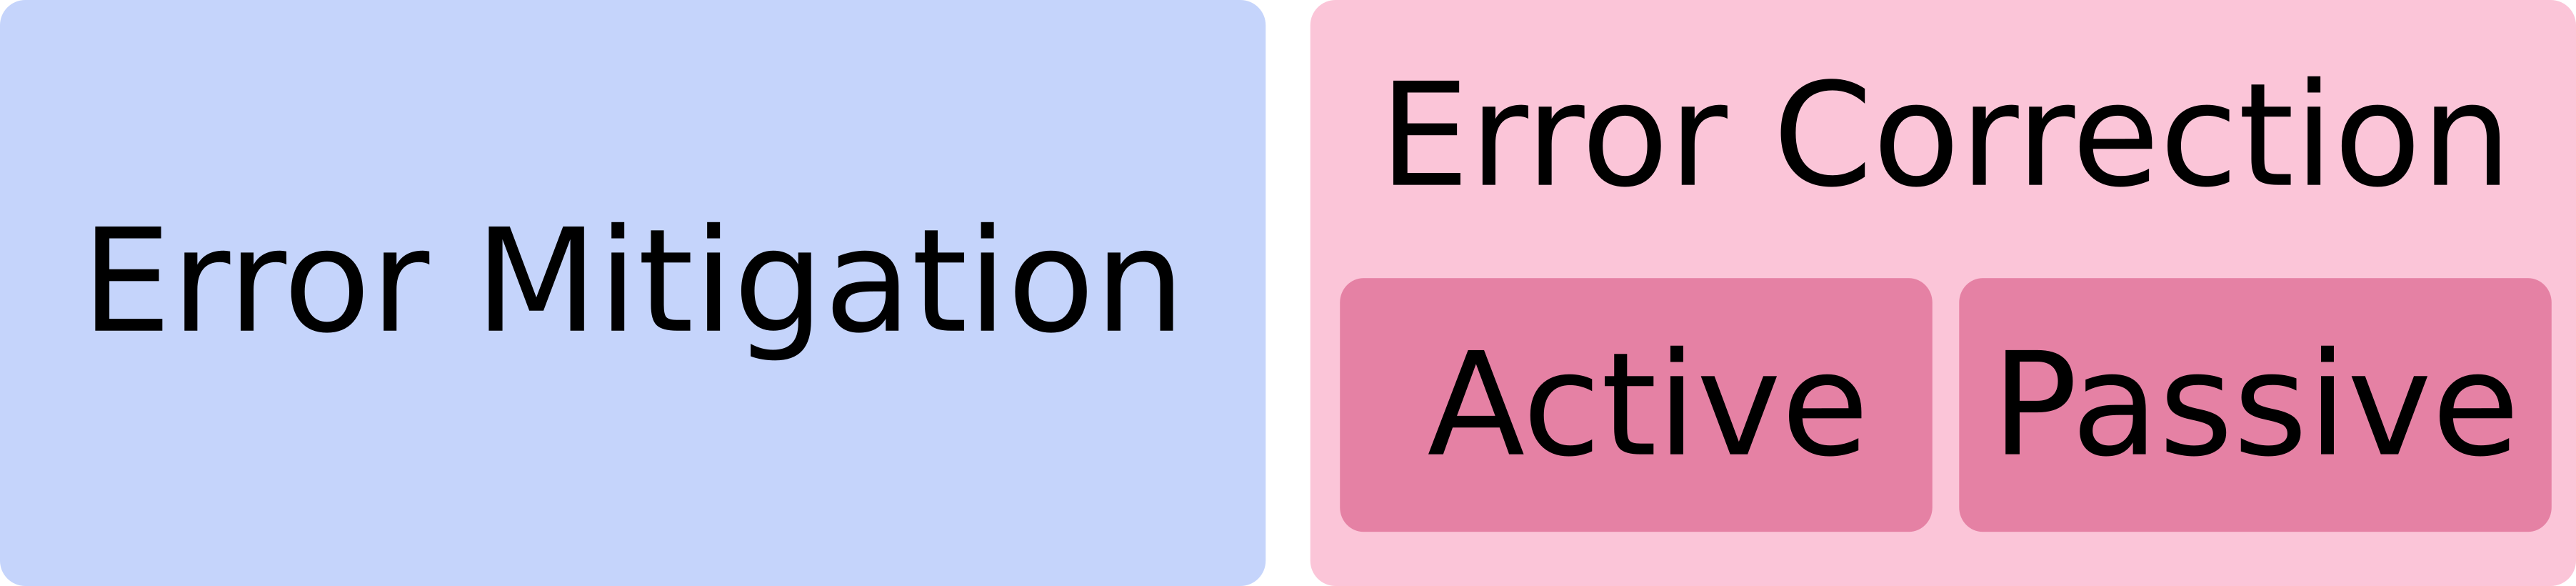
\includegraphics[width=0.6\textwidth]{fig/TypesErrorCorrection.png}
%     \end{center}
% 	\begin{itemize}
% 		\item \textbf{QEM:} Evaluate accurate expectation values of observables on noisy quantum circuits
% 		\item \textbf{QEC:} Build a framework to herald qubits and gates of arbitrary good quality
% 		\begin{itemize}
% 			\item \textbf{Active:} Extracts information about apparent errors and deduces correction operations
% 			\item \textbf{Passive:} Store quantum information in a self correcting way \cite{bacon_operator_2006, berthusen_experiments_2024}
% 		\end{itemize}
% 	\end{itemize}
% \end{frame}

% \begin{frame}{Tackling Quantum Errors}
% 	\begin{center}
%         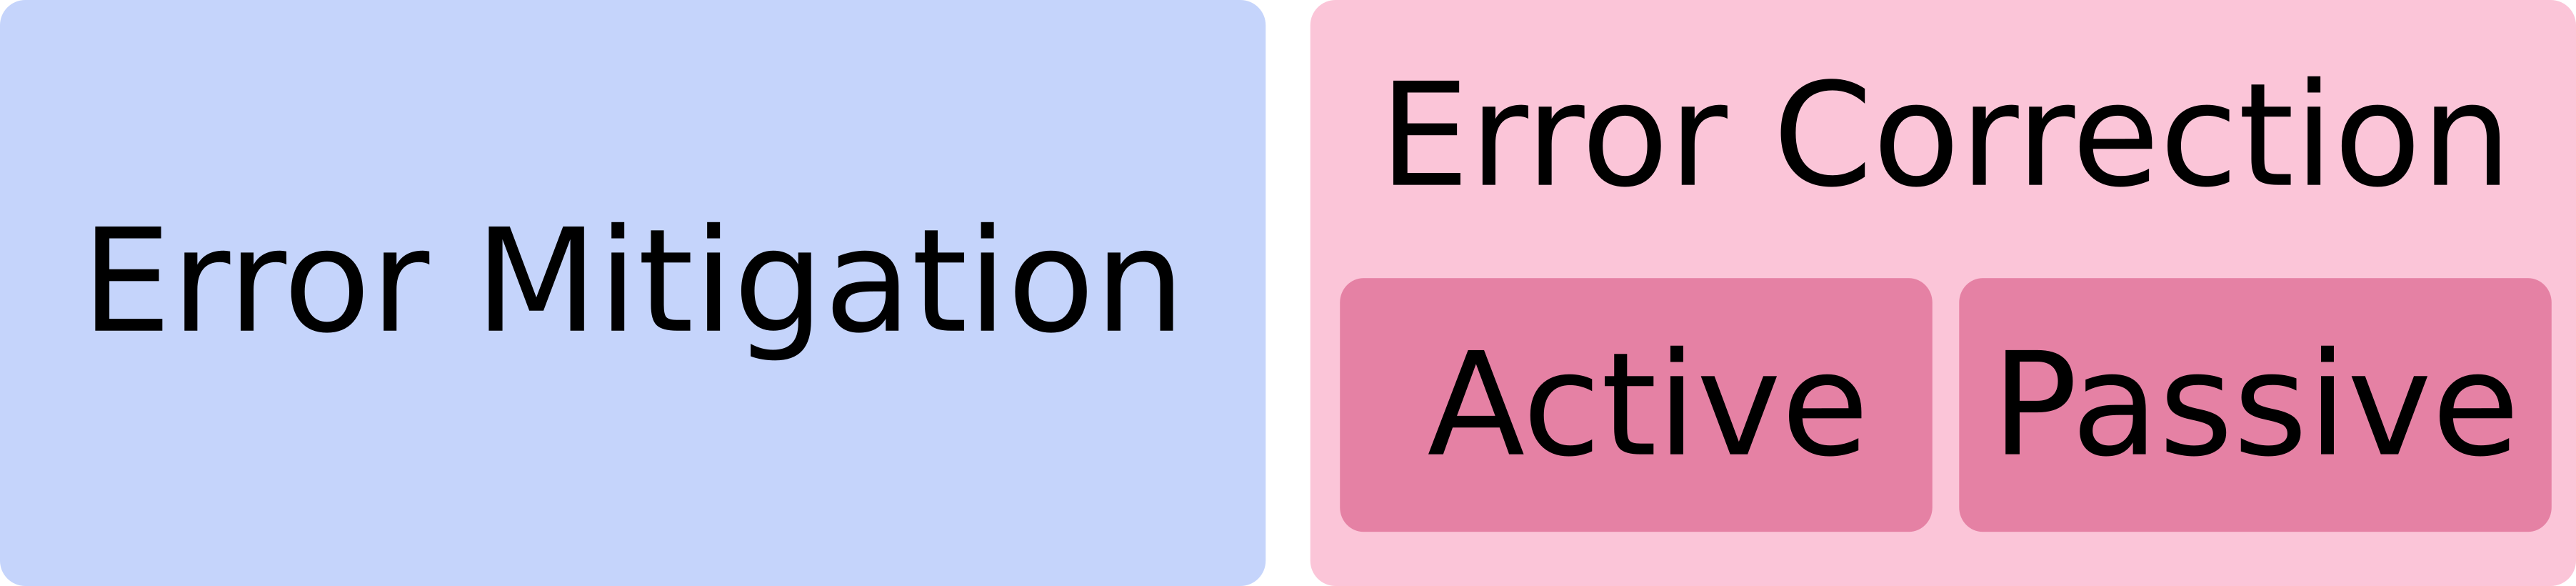
\includegraphics[width=0.6\textwidth]{fig/TypesErrorCorrection.png}
%     \end{center}
% 	\begin{itemize}
% 		\item \textbf{QEM:} Evaluate accurate expectation values by noisy quantum circuits
% 		\item \textbf{QEC:} Obtain qubits and gates of arbitrary good quality
% 		\begin{itemize}
% 			\begin{tcolorbox}[colback=osakared!5!white, colframe=osakared, width=13cm, arc=2mm]
% 			\item \textbf{Active:} Relies on actively measuring information about errors and deducing correction operations
% 			\end{tcolorbox}
% 			\item \textbf{Passive:} Store quantum information in a self correcting way~\cite{bacon_operator_2006, berthusen_experiments_2024}
% 		\end{itemize}
% 	\end{itemize}
% \end{frame}

% \begin{frame}{Experimental Realization}
% 	\vspace{-18pt}
% 	\begin{table}[h]
% 		\fontsize{10pt}{10pt}\selectfont
%         \renewcommand{\arraystretch}{1.5} % Increase row spacing
% 		\begin{tabular}{c|p{3cm}|p{8.5cm}}
% 			\textbf{Year} & \textbf{Author} & \textbf{Contribution} \\
% 			2014 & Nigg et al. & Seven-qubit color code on trapped-ion device and execution of logical single-qubit gates \cite{nigg_quantum_2014} \\
% 			2015 & Kelly et al. &  Nine qubit repetition code on superconducting processor \cite{kelly_state_2015} \\
% 			2020 & Erhard et al. & Lattice surgery generated entanglement of two logical qubits on a ten qubit ion trap device \cite{erhard_entangling_2020} \\
% 			2021 & Ryan et al. & Real time decoding on seven-qubit color code on trapped-ion device and non-Clifford operation \cite{ryan-anderson_realization_2021}\\
% 			2023-24 & Google Quantum AI et al. & Real time decoding and below threshold quantum memory experiments on up to 101 qubits on superconducting processor \cite{google_quantum_ai_suppressing_2023, google_quantum_ai_and_collaborators_quantum_2025}
% 		\end{tabular}
% 	\end{table}
% \end{frame}

% \begin{frame}{Optimal Decoding Methods}
% 	\vspace{-15pt}
% 	\begin{table}[h]
%         \renewcommand{\arraystretch}{1.5} % Increase row spacing
%         \small
% 		\begin{tabular}{c|p{4cm}|p{7cm}}
% 			\textbf{Year} & \textbf{Author} & \textbf{Contribution} \\
% 			2009 & Creighton and Middleton \cite{thomas_exact_2009,thomas_numerically_2013} & Fast algorithm to calculate finite temperature partition functions of planar random bond Ising model based on FKT algortihm \cite{kasteleyn_statistics_1961,temperley_dimer_1961} \\
% 			2013 & Vogel, Li, Wüst, Landau \cite{vogel_generic_2013} & Parallel tempered Wang-Landau algorithm \cite{wang_efficient_2001} for estimating density of states for systems with bounded spectrum \\
% 			2014-21 & Bravyi, Suchara, Vargo and Chubb \cite{bravyi_efficient_2014, chubb_general_2021} & Development of approximate optimal decoding by TN contraction and generalisation to arbitrary 2D stabiliser codes \\
% 		\end{tabular}
% 	\end{table}
% \end{frame}

% \begin{frame}{Noise}
% 	\begin{center}
%         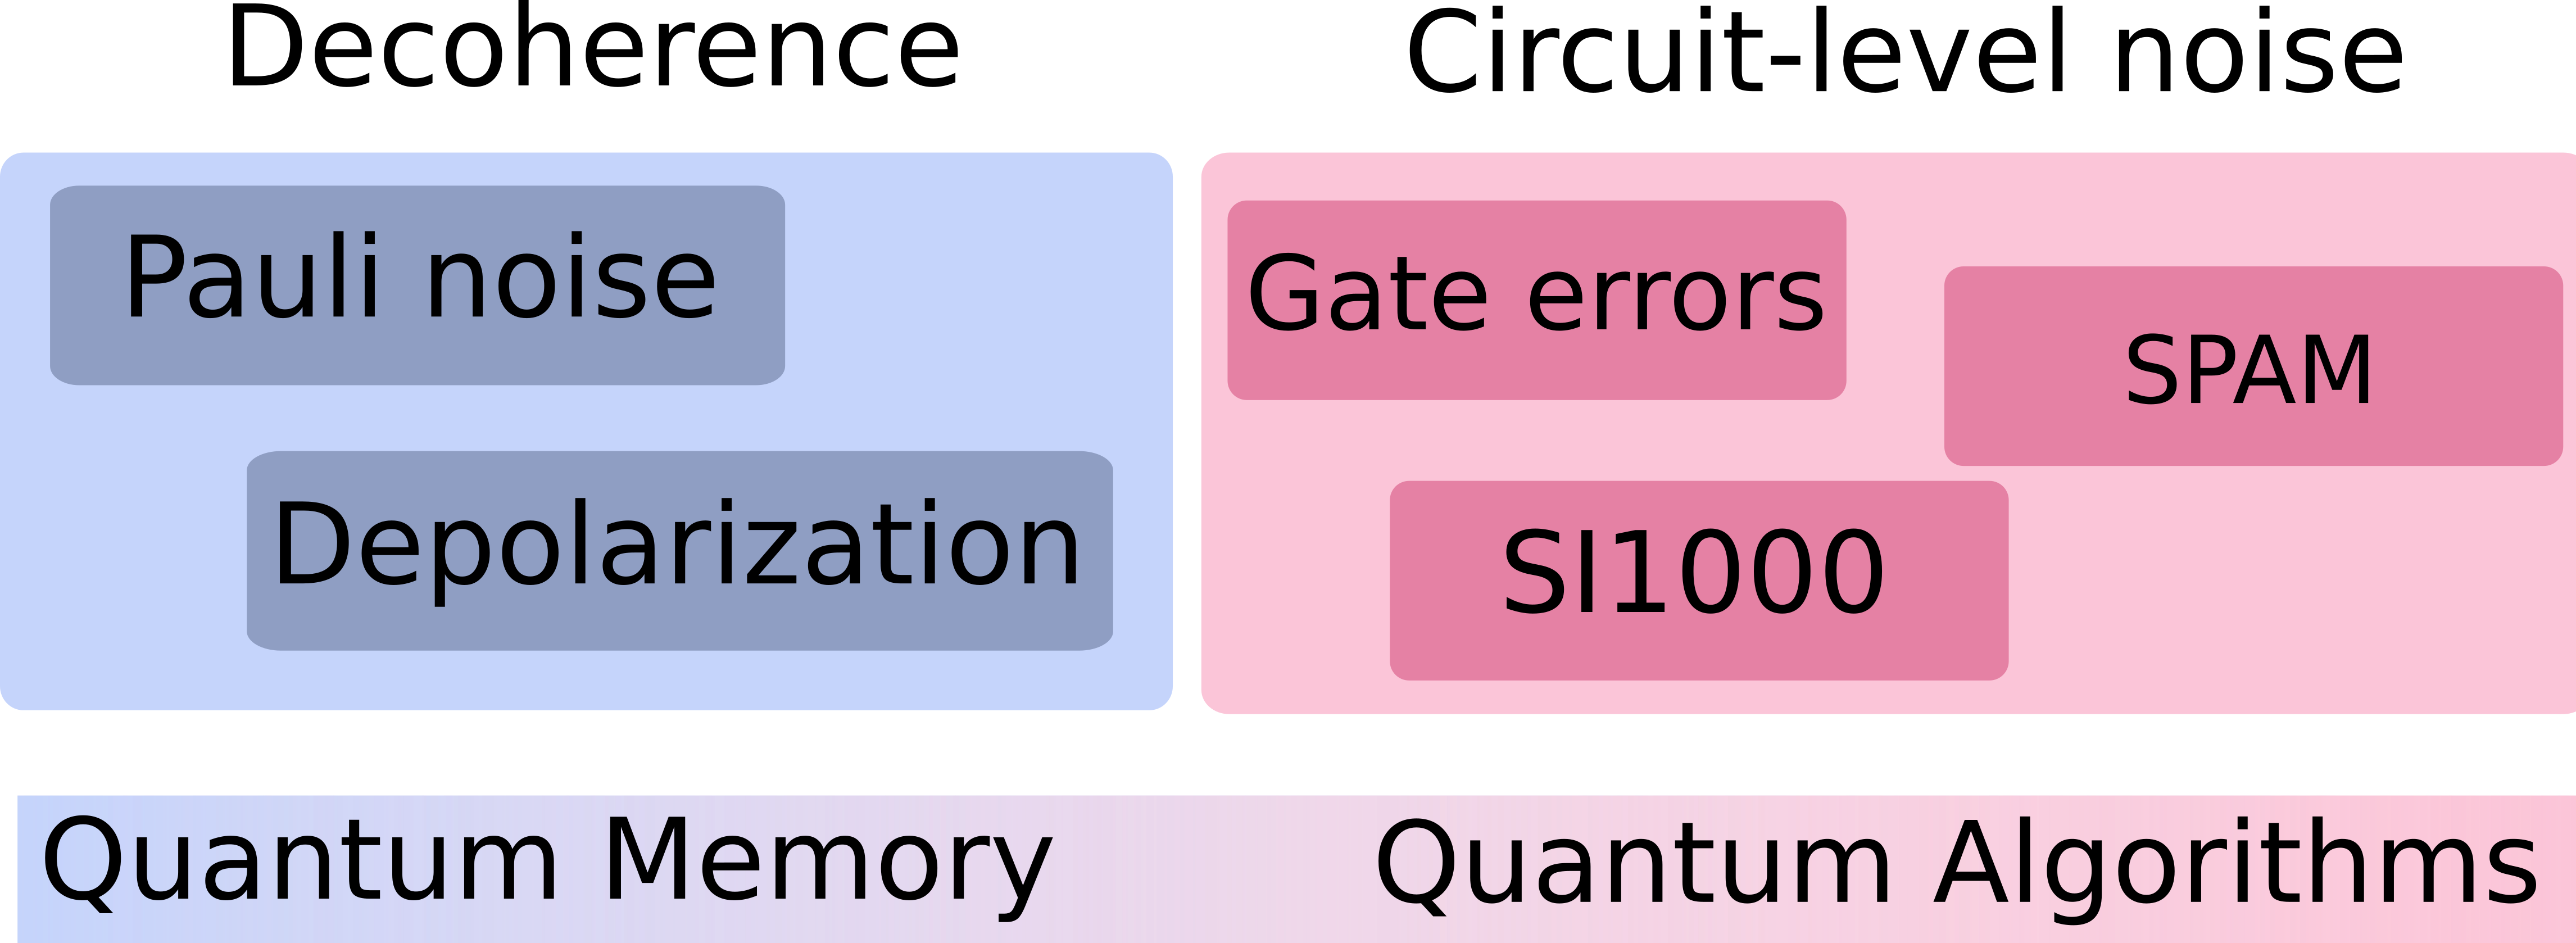
\includegraphics[width=0.6\textwidth]{fig/NoiseTypes.png}
%     \end{center}
% 	\small
% 	\begin{itemize}
% 		\item \textbf{Decoherence:} Interaction with environment evolves idle qubit states stochastically
% 		\item \textbf{Circuit-level Noise:} Caused by imperfect manipualtion of QI:
% 		\begin{itemize}
% 			\item Imperfect implementation of quantum gates causes errors
% 			\item \textbf{S}tate \textbf{P}reparation \textbf{A}nd \textbf{M}easurement errors
% 			\item SI1000: \textbf{S}uperconducting \textbf{I}nspired noise model with \textbf{1000} nanosecond cycle
% 		\end{itemize}
% 	\end{itemize}
% 	\pause
% 	\begin{overlayarea}{\textwidth}{3cm}
% 	\vspace{-8cm}
% 	\hspace{3.5cm}
% 	\begin{tikzpicture}
% 		% Define nodes
% 		\node (A) at (0cm,0cm) {};
% 		\node (B) at (6cm,0cm) {};
% 		\node (C) at (4cm,0cm) {};

% 		% Draw a curved arrow from B to A
% 		\draw[->, bend right=40] (B) to node[above] {Pauli Twirl \cite{geller_efficient_2013}} (A);
% 		\draw[->, bend right=25] (C) to node[above] {} (0.5cm, 0cm);
% 	\end{tikzpicture}
% 	\end{overlayarea}
% \end{frame}


% \begin{frame}{Overview Literature Research}
% 	\begin{center}
% 		\begin{itemize}
% 			\only<1->{
% 			\item Optimal code capacity thresholds
% 			}
% 			\vspace{0.5cm}
% 			\pause
% 			\only<2->{
% 			\item Surface code decoders
% 			}
% 			\vspace{0.5cm}
% 			\pause
% 			\only<3->{
% 			\item Noise effects on code performance
% 			}
% 		\end{itemize}
% 	\end{center}
% \end{frame}


% \begin{frame}{Brief history of QEC}
% 	\vspace{-20pt}
% 	\begin{table}[h]
%         \centering
% 		\renewcommand{\arraystretch}{1.5}
%         \resizebox{\textwidth}{!}{
% 		\begin{tabular}{c|c|p{7cm}}
% 			\textbf{Year} & \textbf{Author} & \textbf{Contribution} \\
% 			1995 & Shor & First quantum error correcting code and threshold theorem~\cite{shor_scheme_1995} \\
% 			1996 & Calderbank, Shor and Steane & Introduction of quantum error correcting codes based on classical codes~\cite{calderbank_good_1996, steane_multiple-particle_1996} \\
% 			1997 & Gottesman & Introduction of stabilizer code framework~\cite{gottesman_stabilizer_1997} \\
% 			1997 & Kitaev & Introduction of the surface code~\cite{hirota_quantum_1997, kitaev_fault-tolerant_2003}\\
% 			2002 & Dennis, Kitaev, Landahl and Preskill & Introduction of statistical mechanics mapping and fault tolerant operations on the surface code~\cite{dennis_topological_2002} \\
% 			2014-15 & Nigg et al. and  Kelly et al. & First experimental realization of small codes \cite{nigg_quantum_2014,kelly_state_2015} \\
% 		\end{tabular}
% 		}
% 	\end{table}
% \end{frame}


% \begin{frame}{Stabilizer Codes}
% 	% \begin{textblock*}{2.5cm}(12.5cm,0.5cm)
% 	% 	
\includegraphics[width=1\textwidth]{fig/QEC_pure_code.png}
% 	% \end{textblock*}
% 	Quality markers: $\frac{k}{n}$, d (, $\omega$ for QLDPC)
% 	\begin{table}[h]
%         \renewcommand{\arraystretch}{1.5} % Increase row spacing
%         \small
% 		\begin{tabular}{c|c|c|c}
% 			\textbf{Code} &  \textbf{n} & \textbf{k} & \textbf{d} \\
% 			\hline
% 			Toric Code \cite{hirota_quantum_1997} & $2d^{2}$ & 2 & d \\
% 			Planar Surface Code & $d^{2} + (L-1)^{2}$ &  1 & d \\
% 			Rotated Surface Code & $d^{2}$ &  1 & d \\
% 			\hline
% 			\pause
% 			Honneycomb Code \cite{landahl_fault-tolerant_2011} & $\frac{3}{4}d^{2}$ + $\frac{1}{4}$ & 1 & d \\
% 			\hline
% 			\pause
% 			Quantum Tanner Code \cite{leverrier_quantum_2022} & n & $\Omega(n)$ & $\Omega(n)$
% 		\end{tabular}
% 	\end{table}
% \end{frame}

% \begin{frame}{Results}
% 	\begin{figure}[h!]
% 		\centering
% 		\begin{minipage}{0.45\textwidth}
% 			\centering
% 			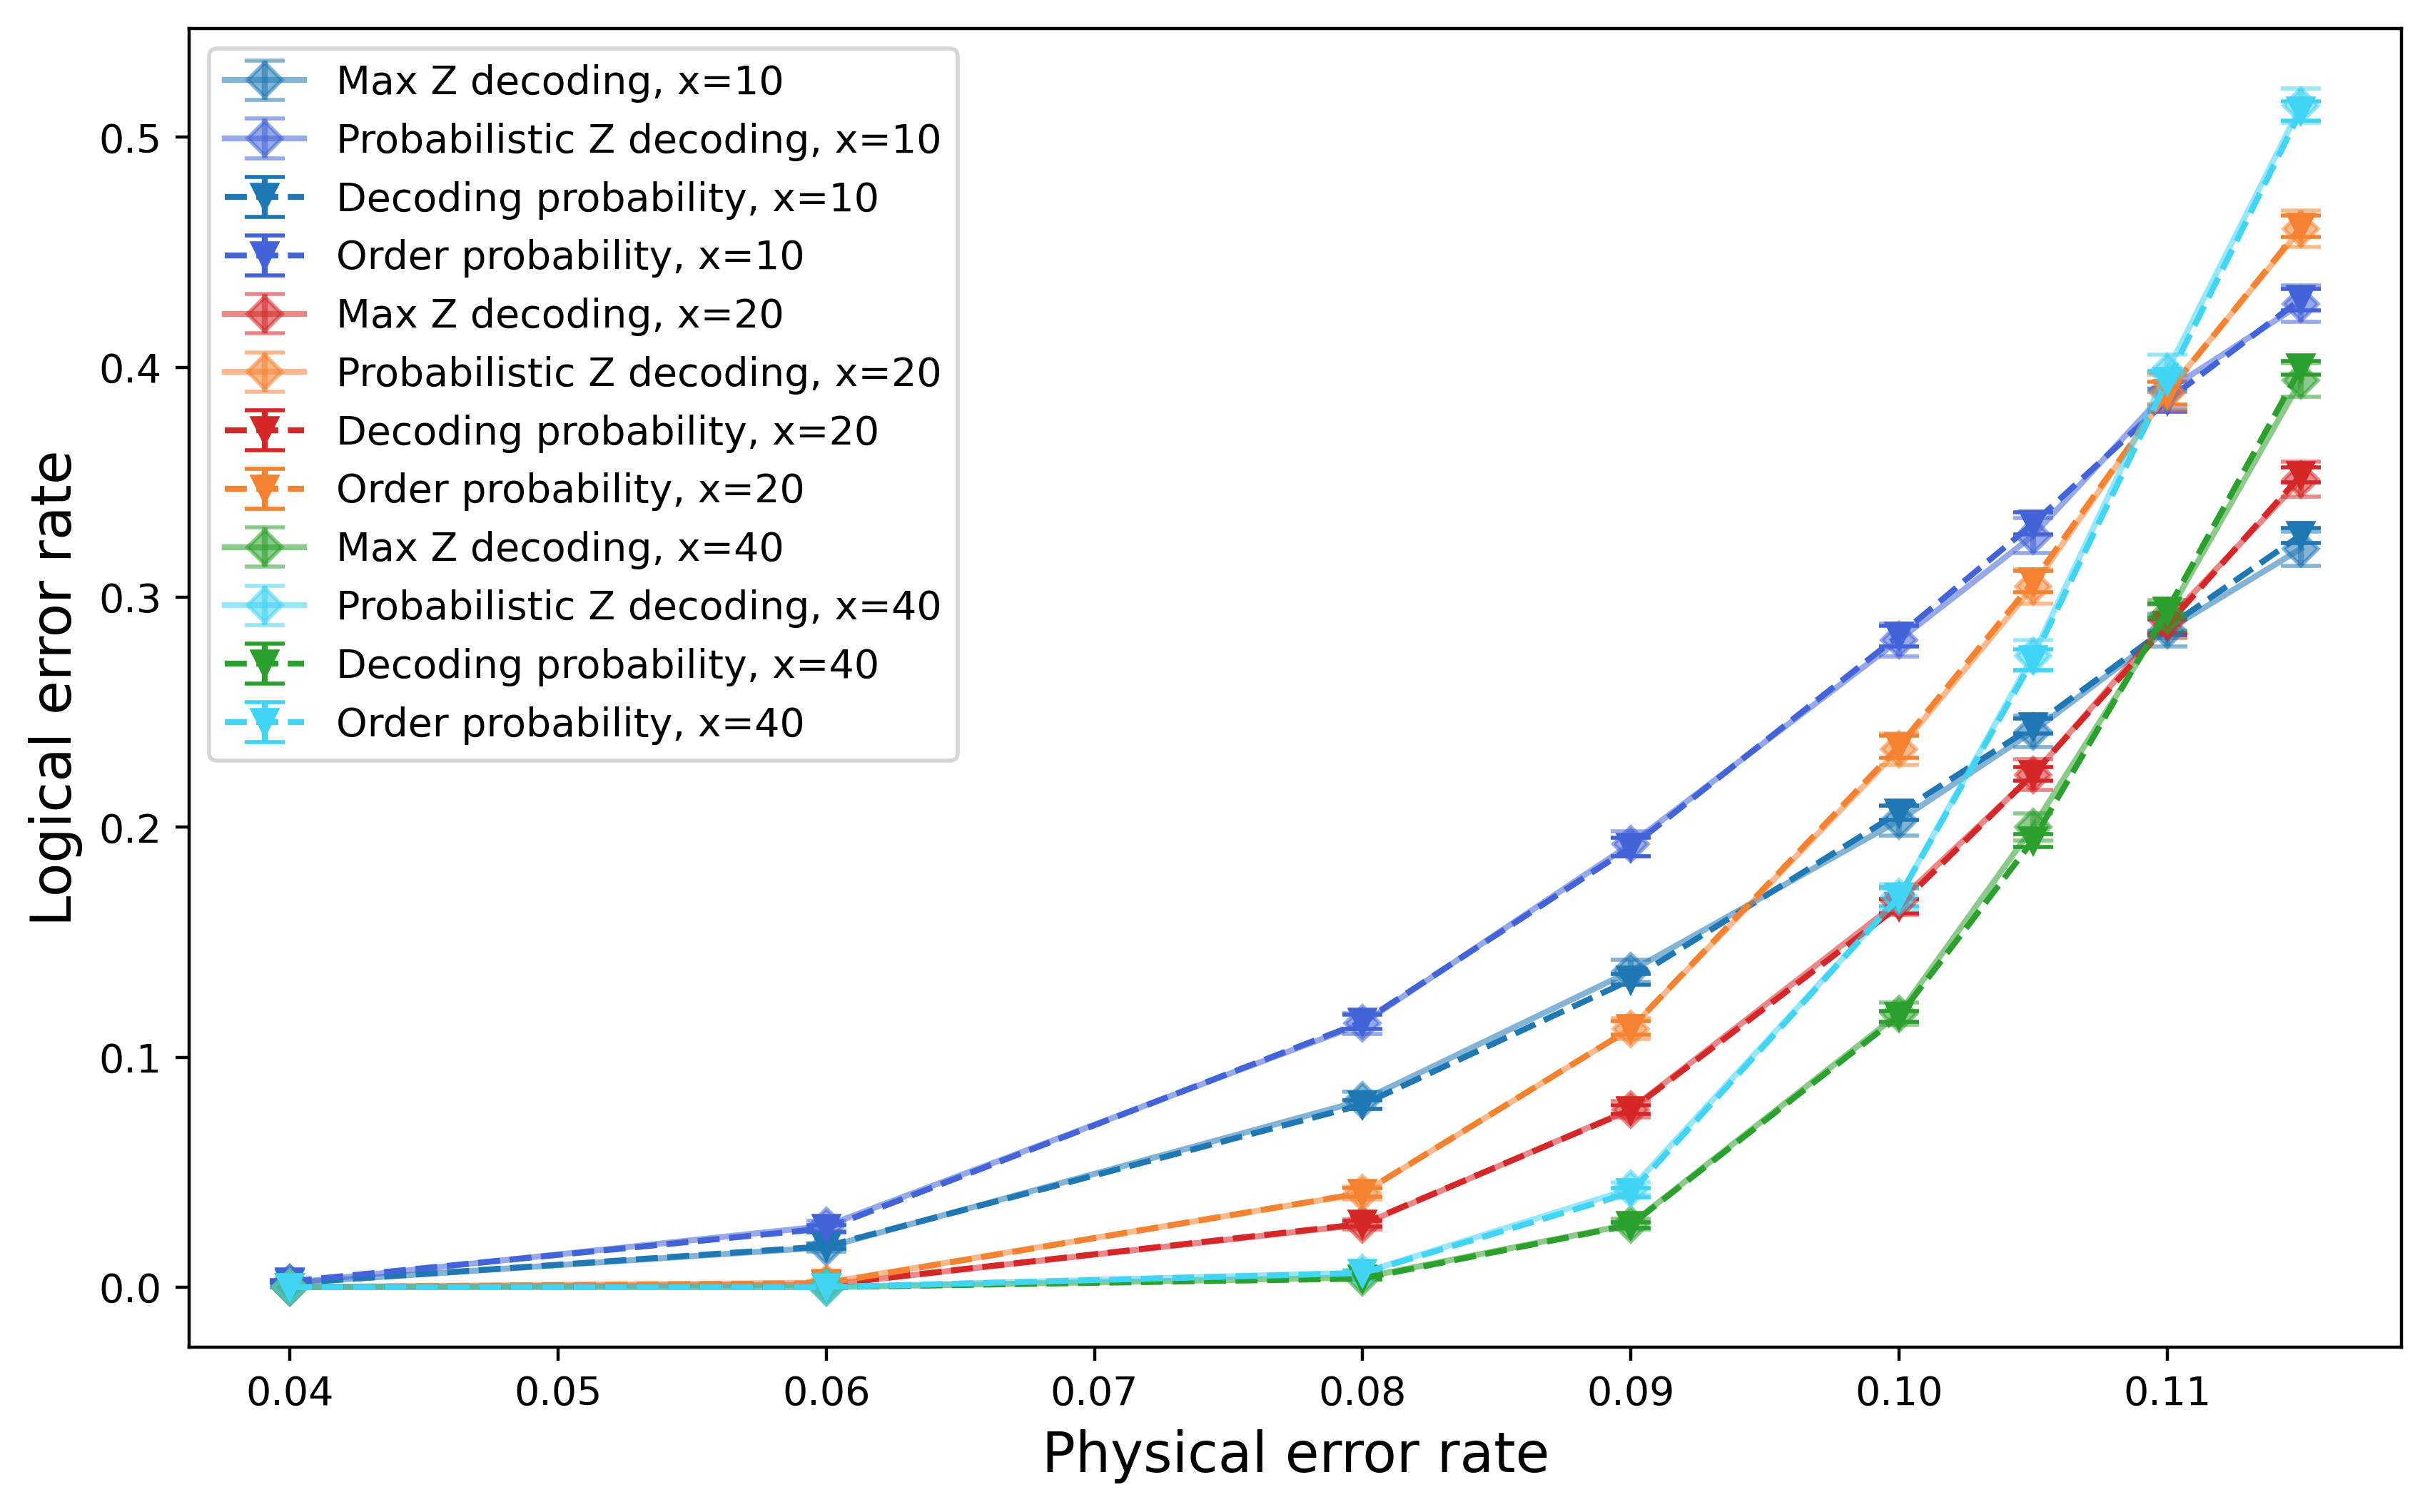
\includegraphics[width=\textwidth]{fig/MaxZ_ProbabilisticZ_OrderProb_DecodingProb_even_T1.png}
% 			\caption{Comparison efficient sampling methods to brute force decoding for even sizes at $T=T_{\text{Nish}}$}
% 		\end{minipage} \hfill
% 		\begin{minipage}{0.45\textwidth}
% 			\centering
% 			\includegraphics[width=\textwidth]{fig/MaxZ_ProbabilisticZ_OrderProb_DecodingProb_odd_T1.png}
% 			\caption{Comparison efficient sampling methods to brute force decoding for odd sizes at $T=T_{\text{Nish}}$}
% 		\end{minipage}
% 	\end{figure}
% \end{frame}

% \begin{frame}{Intermezzo - Groundwork for Results}
%     \begin{minipage}{0.48\textwidth}
%         \small
% 		\textbf{Minimum Energy decoding}\\
% 		Order probability is estimator of success rate
% 		\begin{align*}
% 			&P_{\text{success}}=\lim_{T \to 0}\langle\frac{Z^{T}(E)}{\sum_{l\in L}Z^{T}(l)}\rangle_{s}
% 		\end{align*}
% 		with $P(\bar{l}=l)=\frac{Z^{T}(C_{s}L_{l})}{\sum_{l\in L}Z^{T}(C_{s}L_{l})}$
%     \end{minipage}
% 	\pause
% 	\begin{minipage}{0.48\textwidth}
% 		\small
% 		\textbf{Max Z decoding}
% 		\begin{align*}
% 			&P_{\text{success}}=\langle\frac{Z^{T_{\text{Nishimori}}}(C^{\star}_{s})}{\sum_{l\in L}Z^{T_{\text{Nishimori}}}(C^{\star}_{s}L_{l})}\rangle_{s}
% 		\end{align*}
% 		with $[C^{\star}_{s}(T)]: Z^{T}(C^{\star}_{s})\geq Z^{T}(C_{s})$
%     \end{minipage}
%     \hfill
% 	\pause
% 	\hspace{3cm}
% 	\textcolor{red}{\textbf{Order probability}}
% \end{frame}

% \begin{frame}{Intermezzo - Groundwork for Results}
% 	\only<1-1>{
% 		\begin{textblock*}{16cm}(4cm,1.7cm)
% 			\includegraphics[width=0.4\textwidth]{fig/Toric_code_ex_1.png}
% 		\end{textblock*}
% 	}
% 	\only<2-2>{
% 		\begin{textblock*}{16cm}(4cm,1.7cm)
% 			\includegraphics[width=0.35\textwidth]{fig/Toric_code_ex_2.png}
% 		\end{textblock*}
% 	}
% 	\only<3-3>{
% 		\begin{textblock*}{16cm}(2cm,1.7cm)
% 			\includegraphics[width=0.35\textwidth]{fig/Toric_code_ex_3.png}
% 		\end{textblock*}
% 		\begin{textblock*}{7.5cm}(8cm,2cm)
% 			\textbf{Maximum probability (MP) decoding}\\
% 			\vspace{0.5cm}
% 			% $E_{\text{correction}}=\text{argmax}_{E\in \bar{\mathcal{G}}_{n}}P(E|s)$
% 			Select most probable physical error consistent with the partial error information
% 		\end{textblock*}
% 	}
% 	\only<4-4>{
% 		\begin{textblock*}{16cm}(2cm,1.7cm)
% 			\includegraphics[width=0.35\textwidth]{fig/Toric_code_ex_3.png}
% 		\end{textblock*}
% 		\begin{textblock*}{7.5cm}(8cm,2cm)
% 			\textbf{MP/MWPM decoding}\\
% 			\vspace{0.5cm}
% 			% $E_{\text{correction}}=\text{argmax}_{E\in \bar{\mathcal{G}}_{n}}P(E|s)$
% 			Select physical error which acts on lowest number of qubits non trivially and is consistent with the partial error information
% 	\end{textblock*}
% 	}
% 	\only<5-5>{
% 		\begin{textblock*}{16cm}(2cm,1.7cm)
% 			\includegraphics[width=0.35\textwidth]{fig/Toric_code_ex_6.png}
% 		\end{textblock*}
% 		\begin{textblock*}{7.5cm}(8cm,2cm)
% 			\textbf{MP/MWPM decoding}\\
% 			\vspace{0.5cm}
% 			% $E_{\text{correction}}=\text{argmax}_{E\in \bar{\mathcal{G}}_{n}}P(E|s)$
% 			Select physical error which acts on lowest number of qubits non trivially and is consistent with the partial error information
% 		\end{textblock*}
% 	}
% 	\only<6-6>{
% 		\begin{textblock*}{16cm}(2cm,1.7cm)
% 			\includegraphics[width=0.35\textwidth]{fig/Toric_code_ex_9.png}
% 		\end{textblock*}
% 		\begin{textblock*}{8cm}(8cm,2cm)
% 			\textbf{Maximum likelihood/optimal decoding}\\
% 			Takes redundancy into account
% 		\end{textblock*}
% 	}
% 	\only<6-6>{
% 		\begin{textblock*}{16cm}(2cm,1.7cm)
% 			\includegraphics[width=0.35\textwidth]{fig/Toric_code_ex_9.png}
% 		\end{textblock*}
% 		\begin{textblock*}{8cm}(8cm,2cm)
% 			\textbf{Maximum likelihood/optimal decoding}\\
% 			Takes redundancy into account
% 		\end{textblock*}
% 	}
% 	% \only<6-6>{
% 	% \begin{textblock*}{16cm}(4cm,1.7cm)
% 	% 	\includegraphics[width=0.35\textwidth]{fig/Toric_code_ex_7.png}
% 	% \end{textblock*}
% 	% \begin{textblock*}{6cm}(10cm,2cm)
% 	% 	\textbf{success!} \\ But didnt take degeneracy into account
% 	% \end{textblock*}
% 	% }
% 	% \only<7-7>{
% 	% \begin{textblock*}{16cm}(2cm,1.7cm)
% 	% 	\includegraphics[width=0.35\textwidth]{fig/Toric_code_ex_2.png}
% 	% \end{textblock*}
% 	% \begin{textblock*}{8cm}(8cm,2cm)
% 	% 	\textbf{Maximum likelihood/optimal decoding}\\
% 	% 	$C_{s} \in \mathcal{G}_{n}$ compatible with $s$\\
% 	% 	$[C_{s}]=SC_{s}$ \\
% 	% 	$s \mapsto C_{s}L_{\delta(s)}$ with \\
% 	% 	$\delta(s) = \arg\max_{l\in L}P([C_{s}L_{l}])$
% 	% \end{textblock*}
% 	% }
% 	\only<8-8>{
% 		\begin{textblock*}{16cm}(2cm,1.7cm)
% 			\includegraphics[width=0.35\textwidth]{fig/Toric_code_ex_8.png}
% 		\end{textblock*}
% 		\begin{textblock*}{8cm}(8cm,2cm)
% 			\textbf{Maximum likelihood/optimal decoding}\\
% 			$C_{s} \in \mathcal{G}_{n}$ compatible with $s$\\
% 			$[C_{s}]=SC_{s}$ \\
% 			$s \mapsto C_{s}L_{\delta(s)}$ with \\
% 			$\delta(s) = \arg\max_{l\in L}P([C_{s}L_{l}])$\\
% 			$\phantom{\delta(s)} \overset{\text{\cite{dennis_topological_2002}}}{=} \arg\max_{l\in L}Z^{T_{\text{Nishimori}}}(C_{s}L_{l})$
% 		\end{textblock*}
% 	}
% 	\only<9-9>{
% 		\begin{textblock*}{16cm}(2cm,1.7cm)
% 			\includegraphics[width=0.35\textwidth]{fig/Toric_code_ex_8.png}
% 		\end{textblock*}
% 		\begin{textblock*}{8cm}(8cm,2cm)
% 			\textbf{Max Z decoding at temperature T}\\
% 			$C_{s} \in \mathcal{G}_{n}$ compatible with $s$\\
% 			$[C_{s}]=SC_{s}$ \\
% 			$s \mapsto C^{\star}_{s}(T)\equiv C_{s}L_{\delta(s)}$ with \\
% 			$\delta(s) = \arg\max_{l\in L}Z^{T}(C_{s}L_{l})$\\
% 			\vspace{0.8cm}
% 			\textbf{Probabilistic Z decoding at temperature T}:\\
% 			$\overline{\delta(s)}$ with $P(\overline{\delta(s)} = l\in L)=\frac{Z^{T}(C_{s}L_{l})}{\sum_{l\in L}Z^{T}(C_{s}L_{l})}$
% 		\end{textblock*}
% 	}
% 	\only<10-10>{
% 		\begin{textblock*}{16cm}(2cm,1.7cm)
% 			\includegraphics[width=0.35\textwidth]{fig/Toric_code_ex_8.png}
% 		\end{textblock*}
% 		\begin{textblock*}{8cm}(8cm,2cm)
% 			\textbf{Max Z decoding at temperature T}\\
% 			$C_{s} \in \mathcal{G}_{n}$ compatible with $s$\\
% 			$[C_{s}]=SC_{s}$ \\
% 			$s \mapsto C^{\star}_{s}(T)\equiv C_{s}L_{\delta(s)}$ with \\
% 			$\delta(s) = \arg\max_{l\in L}Z^{T}(C_{s}L_{l})$\\
% 			\vspace{0.8cm}
% 			\textbf{Probabilistic Z decoding at temperature T}:\\
% 			$\overline{\delta(s)}$ with $P(\overline{\delta(s)} = l\in L)=\frac{Z^{T}(C_{s}L_{l})}{\sum_{l\in L}Z^{T}(C_{s}L_{l})}$\\
% 			\vspace{0.8cm}
% 			Estimation of Z by REWL and FKT algorithm
% 		\end{textblock*}
% 	}
% 	% \only<6-6>{
% 	% \begin{textblock*}{16cm}(4cm,1.7cm)
% 	% 	\includegraphics[width=0.35\textwidth]{fig/Toric_code_ex_4.png}
% 	% \end{textblock*}
% 	% }
% 	% \only<7-7>{
% 	% \begin{textblock*}{16cm}(4cm,1.7cm)
% 	% 	\includegraphics[width=0.35\textwidth]{fig/Toric_code_ex_5.png}
% 	% \end{textblock*}
% 	% }
% \end{frame}

% \begin{frame}{Definitions}
% 	\begin{minipage}{0.48\textwidth}
% 		\small
% 		\textbf{Z decoding at T}
% 		\begin{align*}
% 			&P_{\text{success}}=\sum_{s}P(s)P_{\text{success}}(s)\\
% 			&P_{\text{success}}(s)=P(C^{\star}_{s}(T))=\frac{Z^{T_{\text{Nishimori}}}(C^{\star}_{s})}{\sum_{l\in L}Z^{T_{\text{Nishimori}}}(C^{\star}_{s}L_{l})}\\
% 			&\Rightarrow P_{\text{success}}=\langle\frac{Z^{T_{\text{Nishimori}}}(C^{\star}_{s})}{\sum_{l\in L}Z^{T_{\text{Nishimori}}}(C^{\star}_{s}L_{l})}\rangle_{s}
% 		\end{align*}
% 		with $[C^{\star}_{s}(T)]: Z^{T}(C^{\star}_{s})\geq Z^{T}(C_{s})$
%     \end{minipage}
% \end{frame}

% \begin{frame}{Intermezzo - Groundwork for Results}
% 	\begin{minipage}{0.48\textwidth}
% 		\small
% 		\textbf{Max Z decoding at T}
% 		\begin{align*}
% 			&P_{\text{success}}=\langle\frac{Z^{T_{\text{Nishimori}}}(C^{\star}_{s})}{\sum_{l\in L}Z^{T_{\text{Nishimori}}}(C^{\star}_{s}L_{l})}\rangle_{s}
% 		\end{align*}
% 		with $[C^{\star}_{s}(T)]: Z^{T}(C^{\star}_{s})\geq Z^{T}(C_{s})$
%     \end{minipage}
%     \hfill
% 	\pause
%     \begin{minipage}{0.48\textwidth}
%         \small
% 		\textbf{Probabilistic Z decoding at T}
% 		\begin{align*}
% 			&P_{\text{success}}=\langle\frac{Z^{T}(C_{s}L_{\bar{l}})}{\sum_{l\in L}Z^{T}(C_{s}L_{l})}\rangle_{s}
% 		\end{align*}
% 		with $P(\bar{l}=l)=\frac{Z^{T}(C_{s}L_{l})}{\sum_{l\in L}Z^{T}(C_{s}L_{l})}$
%     \end{minipage}
% 	\pause
% 	\textcolor{red}{\textbf{Decoding probability}}
% 	\hspace{3cm}
% 	\textcolor{red}{\textbf{Order probability}}
% \end{frame}



% \begin{frame}{Recent advancements in QEC}
% 	\begin{tcolorbox}[colback=osakared!5!white, colframe=osakared, width=13cm, arc=2mm]
% 		\textbf{Google Quantum AI} Performed quantum memory experiments with surface codes below the error correction threshold.
% 	\end{tcolorbox}
% 	\vspace{10pt}
% 	$\Rightarrow$ Their hardware is in regime where code performance can be increased by increased system size\\
% 	\pause
% 	\vspace{10pt}
% 	Moreover they were able to improve the decoder performance by adapting to device noise.
% 	% The scaling of the physical qubit count from 72 to 101 qubits resulted in a suppression of the logical error rate by a factor of roughly two. \\
% 	% their optimized mwpm decoder was able to decode in real time while a neural network decoder only acted as offline decoder due to fast processor cycle duration
% \end{frame}

% \begin{frame}{Problem statement}
% 	\includegraphics[width=0.4\textwidth]{fig/resource_intensive_decoder_dev.png}
% 	\only<1>{\hspace{20pt}\raisebox{35pt}{$\huge \Rightarrow$ \textbf{Only do it for promising codes}}}
% 	\only<2->{
% 		\hspace{2pt}
% 		\raisebox{18pt}{\includegraphics[width=0.08\textwidth]{fig/arrows.png}}
% 		\hspace{5pt}
% 		\includegraphics[width=0.4\textwidth]{fig/promising_codes.png}\\
% 	}
% 	\vspace{10pt}
% 	\only<3->{
% 	\textbf{Optimal code performance estimates can aid this process!}
% 	\begin{itemize}
% 		\only<3->{\item \textbf{Code selection:} Hardware specific simulation of optimal code performance makes error correcting codes comparable.}
% 		\only<4>{\item \textbf{Decoder optimization:} Estimation of optimal code performance shows upper limit for decoder optimization.}
% 	\end{itemize}
% 	}
% \end{frame}

% \begin{frame}{Results}
% 	\only<1->{
% 	\begin{itemize}
% 		\only<1->{\item Developed a hardware adaptive framework for optimal code performance estimation}
% 		\only<2->{\item Applied framework to estimate optimal performance of the toric code under bitflip noise}
% 	\end{itemize}
% 	}
% 	\pause
% 	\vspace{-15pt}
% 	\begin{center}
% 		\includegraphics[width=0.6\linewidth]{fig/FKT threshold Temp=1.0.png}
% 	\end{center}
% 	% We produced estimates for the error correction threshold of the toric code under bitflip noise. \\
% 	% Here we can clearly see the two regimes which are governed by different scaling behavior with the qubit count of the error correcting code. \\
% \end{frame}

% \begin{frame}{Results}
% 	Improved performance of a fast decoder and compared to optimal decoder performance: % maximum likelihood decoding is NP hard
% 	\begin{center}
% 		\includegraphics[width=0.6\linewidth]{fig/Improved decoder 10.png}
% 	\end{center}
% \end{frame}

% \begin{frame}{Results}
% 	Investigation of noise informed decoder:
% 	\begin{center}
% 		\includegraphics[width=0.5\linewidth]{fig/noise_aware.png}
% 	\end{center}
% \end{frame}

% \begin{frame}{Summary}
% 	\begin{center}
% 		\includegraphics[width=0.8\linewidth]{fig/summary.png}
% 	\end{center}
% \end{frame}

% \begin{frame}{Work plan}
% 	\begin{table}[h]
% 		\fontsize{8pt}{9pt}\selectfont
% 		\center
% 		{\renewcommand{\arraystretch}{2}
% 		\begin{tabular}{l@{\hspace{1em}}p{4.5cm}p{3cm}l@{\hspace{1em}}p{1.7cm}}
%             \toprule
%             Authorship & Title & Type  & Year & Status   \\
%             \midrule
%             1st-author & Estimating optimal performance in stabilizer and subsystem codes & Physical Review A & 2025 & submission March-April \\
% 			co-author & Parallelization of Shor's algorithm & IEEE Transactions on Quantum Engineering & 2025 & submission February \\
%             to be discussed & Extending current results to realistic noise models & Journal & 2025-26 & Future work \\
% 			to be discussed & QuaSA: Error dynamics of Quantum Memory & Journal & 2026 & Future work \\
%             \bottomrule
%         \end{tabular}
% 		}
% 	\end{table} \vfill
% \end{frame}
